\documentclass[10pt]{book}
\usepackage[letterpaper,top=2.5cm,bottom=2.5cm,left=2.5cm,right=2.5cm]{geometry}
\usepackage{makeidx}
\usepackage{graphicx}
\usepackage{multicol}
\usepackage{float}
\usepackage{listings}
\usepackage[usenames,dvipsnames]{color}
\usepackage{amsmath}
\usepackage{ifthen}
\usepackage[table]{xcolor}
\usepackage{textcomp}
\usepackage{alltt}
\usepackage{ifpdf}
\ifpdf
\usepackage[pdftex,
            pagebackref=true,
            colorlinks=true,
            linkcolor=blue,
            unicode
           ]{hyperref}
\else
\usepackage[ps2pdf,
            pagebackref=true,chapter
            colorlinks=true,
            linkcolor=blue,
            unicode
           ]{hyperref}
\usepackage{pspicture}
\fi
\usepackage[utf8]{inputenc}
\usepackage{mathptmx}
\usepackage{sectsty}

\usepackage{mathptmx}
\usepackage[scaled=.90]{helvet}
\usepackage{courier}
\usepackage{sectsty}
\usepackage[titles]{tocloft}
\usepackage{prettyref}
\usepackage{mdwlist}
\usepackage{enumitem}
\usepackage{framed, color}  %SP
\usepackage{pbox} %SP
\definecolor{shadecolor}{rgb}{0.92,0.92,0.92}

\usepackage{draftcopy}
\usepackage{fancyhdr}
\usepackage{wrapfig}

\usepackage[nolist]{acronym}
%%%%%%%%%%%%%%%Borrowed from MPI Spec%%%%%%%%

% Version as of April 8, 1997

%   ----------------------------------------------------------------------
%   osh.tex inspired by mpi-macs.tex  --- man page macros,
%                discuss, missing, mpifunc macros
%
% ----------------------------------------------------------------------

% TeX if definitions.  These are defined here so (a) there is one place to
% change the defaults and (b) so that they can be changed by reading a
% configuration file
% Control the use of color
\newif\ifusecolor
\usecolortrue
% Control whether changes are highlighted
\newif\ifshowchange
\showchangetrue
% Control whether deleted text is shown
\newif\ifshowdelete
\showdeletetrue
% Control the use of change "bars" (really markers).  Note that
% both changetrue and changebarstrue must not be set
\newif\ifchangebars
\changebarsfalse
% Control whether tickets are indicated in the margins (or inline, when 
% they occur in inner mode.  Note that this has no effect if \showchangetrue
% is not set
\newif\ifshowtickets
\showticketstrue
% For publisher's additions in the printed book
\newif\ifbookprinting
\bookprintingfalse

%
% There are a number of features that are controlled by LaTeX if commands.
% This step allows you to control these through a configuration file
% This file should contain valid LaTeX commands, including comments (using
% the standard % character for comments)
%
% Known commands include:
% \showchangetrue   - Show changes/additions (from a previous version)
% \showdeletetrue   - Show deleted text (deleted from a previous version)
% \changebarstrue   - Show change "bars" around changes (really begin/end
%                     markers in the output file)
% \usecolortrue     - Use color to show changes
% 
\newread\cfgin

%
% General text color update macros
% These permit the use of nesting of the color changes, as well as
% a "do not change" option
%
\ifusecolor
\definecolor{orange}{rgb}{1,0.5,0}
\definecolor{purple}{rgb}{0.8,0,1}
\let\XA=\expandafter
% Definition for "Use current color"
\def\ColorSame{same}
% Create a stack that is 5 deep (no arrays in TeX)
\def\ColorS{black}
\def\ColorSi{same}
\def\ColorSii{same}
\def\ColorSiii{same}
\def\ColorSiiii{same}
% Stack pointer
\newcount\ColorStackP 
\ColorStackP=0
% Push a new color
\def\ColorPush#1{%
\global\advance\ColorStackP 1\relax%
\ifnum\ColorStackP>4\message{Font Color stack too deep}\fi%
\ifnum\ColorStackP=1\global\def\ColorSi{#1}\else
\ifnum\ColorStackP=2\global\def\ColorSii{#1}\else
\ifnum\ColorStackP=3\global\def\ColorSiii{#1}\else
\ifnum\ColorStackP=4\global\def\ColorSiiii{#1}%
\fi
\fi
\fi
\fi
\def\ColorCur{#1}%
\ifx \ColorCur\ColorSame \relax\else \color{#1}\fi
}
% Pop that color
\def\ColorPop{\global\advance\ColorStackP -1\relax%
\ifnum\ColorStackP<0\message{Font Color stack < 0}\fi%
\ifnum\ColorStackP=0\def\ColorCur{\ColorS}\else
\ifnum\ColorStackP=1\def\ColorCur{\ColorSi}\else
\ifnum\ColorStackP=2\def\ColorCur{\ColorSii}\else
\ifnum\ColorStackP=3\def\ColorCur{\ColorSiii}\else
\ifnum\ColorStackP=4\def\ColorCur{\ColorSiiii}%
\fi
\fi
\fi
\fi
\fi%\typeout{cur = \ColorCur and same = \ColorSame}%
\ifx\ColorCur\ColorSame\relax\else\color{\ColorCur}\fi%
}
% A synonym for color that is controlled by the \usecolortrue command
\def\Color#1{\color{#1}}
\else
\def\ColorPush#1{}
\def\ColorPop{}
\def\Color#1{}
\fi % \ifusecolor

\ifshowdelete
\def\nocomment{\catcode`\%=9}
\def\restorecomment{\catcode`\%=14}
\else
\let\nocomment=\relax
\let\restorecomment=\relax
\fi

\ifchangebars
\def\BegChange{\begchange}
\def\EndChange{\endchange}
\else
\let\BegChange=\relax
\let\EndChange=\relax
\fi

\ifshowchange
%
% Use margin par for the ticket number unless marginpar won't work, in 
% which case inline the ticket number.  To do more would require special
% code for the TeX output routine, which isn't worth it for what we need 
% here.
% Note that the changebars and the ticket both use marginpar, and if both 
% are used at the same time, LaTeX may run out of floats
\ifchangebars
\def\ticket#1{\relax}
\else
\ifshowtickets
\def\ticket#1{\ifinner[ticket#1.]\else\protect\marginpar[\mbox{\hbox to \marginparwidth{\hss ticket#1.\hspace{30pt}}}]{\hbox to \marginparwidth{\hspace{30pt}ticket#1.\hss}}\fi}
\else
\def\ticket#1{\relax}
\fi % showtickets
\fi % changebars
\fi

% fancyvrb defines Verbatim, which is a slightly better Verbatim environment
% Regrettably, the key feature needed, commandchars, does not work correctly
% in our environment (it doesn't accept arbitrary grouping characters).
% See README-2.2 for instructions on using Verbatim along with the above 
% update macros.
%\usepackage{fancyvrb}


\def\snir{\relax}
\def\rins{\relax}


% To make the changes without showing the location or old source: 
%    \newcommand{\CHANGE}[2]{}
%    \newcommand{\INTO}[1]{#1}
%    \newcommand{\ADD}[2]{#2}
 %   \newcommand{\DELETE}[2]{}

 
% available: red green blue cyan yellow magenta
 \def\RVWCAP/{}                                                       % shortcut for Review item 23.a - capitalization of titles (in \section}
% \def\RVWcap/{\mpiiidotiMergeFromREVIEWbegin{23.a}}                   % shortcut for Review item 23.a - capitalization of titles
\def\RVWcap/{}                                                       % shortcut for Review item 23.a - capitalization of titles
 
\def\OnlyForAutomaticAnnexGeneration#1{}% deleting the content were the macro is used; but preserving it for the Annex

 
% This macro enables that all "_" (underscore) characters in the pfd
% file are searchable, and that cut&paste will copy the "_" as underscore. 
% Without the following macro, the \_ is treated in searches and cut&paste
% as a " " (space character). 
% This macro does not modify the behavior of _ in math or in verbatim 
% environments. In verbatim environments, the "_" is always treated
% as a searchable character.
%
\DeclareRobustCommand{\_}{\texttt{\char`\_}} 
% 

% From MPI-2.0
% ------------
 
% Place some penalty for doing the break
% The penalty for a ``\gb'' should be greater than a \hyphenpenalty.
% \hyphenpenalty is 50 in plain.tex.
\def\gb{\penalty10000\hskip 0pt plus 8em\penalty4800\hskip 0pt plus-8em%
\penalty10000}

% A theorem-like environment for code Examples (S. Otto) see Lamport, pg 58
%
% Note that because we use a theorem environment that resets the counter
% with every chapter, pdflatex will issue a warning for each example that
% has the same number as an example in another chapter.  This is too hard
% to fix (the easist way is to not use the theorem environment and roll
% a custom environment, including adding the necessary low-level commands
% for the pdf link support.
%\newtheorem{example}{Example}[chapter]
% Theorems have \em text; we want \rm.  The easiest way to fix this, 
% since we are not using Theorems, is to change the @begintheorem macro
\makeatletter
\def\@begintheorem#1#2{\rm \trivlist \item[\hskip \labelsep{\bf #1\ #2}]}
\makeatother
% Use \exindex{MPI\_FUNC} to generate an index entry for MPI
% functions/constants 
%\newcommand{\exindex}[1]{\relax}
%\newcommand{\exindex}[1]{\index{EXAMPLES:#1}}

% a couple of commands from Marc Snir, modified S. Otto

%\newlength{\discussSpace}
%\setlength{\discussSpace}{.4cm}

%\newenvironment{funcdef}[1]{
%    \vspace{\codeSpace}
%    \noindent
%    \samepage
%    \hangindent 7em\hangafter=1
%    {\funcNoIndex{{\prefix}#1}}\mpifuncmainindex{#1}
%    \MPIfunclist
%}{\end{list} \vspace{\codeSpace}}

%\newcommand{\function}[1]{{\raggedright \hangindent 7em\hangafter=1\tt #1 \par \vspace{0.1in}}}
%\newcommand{\CM}{Communication Middleware}
% Watermark
%
% For release please remove waternark and lino
% DRAFT !!!
\usepackage{draftwatermark}

% max depth for table of content
\setcounter{tocdepth}{4}
% set path to figures
\graphicspath{{./figures/}}

\usepackage{xspace}
\newcommand{\openshmem} {\mbox{OpenSHMEM}\xspace % \textsuperscript{{\small \texttrademark}}
}
\newcommand{\insertDocVersion}{1.1 DRAFT}
\newcommand{\deprecate}[1]{\textcolor{Gray}{#1 (deprecated)}}
%\renewcommand\linenumberfont{\normalfont\scriptsize\sffamily}

\hypersetup{pdftitle={\openshmem Specification Draft},
 pdfauthor={HPC Tools, University of Houston},
 pdfkeywords={Specification, Draft, \openshmem, SHMEM, PGAS, Partitioned, Global, Address, Gasnet, Parallel}}
 
\definecolor{gray}{rgb}{0.92,0.92,0.92}
\lstset{ %
  breakatwhitespace=false,         % sets if automatic breaks should only happen at whitespace
  basicstyle=\ttfamily\footnotesize,
  %identifierstyle=\ttfamily\itshape,
  breaklines=true,                 % sets automatic line breaking
  escapeinside={\%*}{*)},          % if you want to add LaTeX within your code
  extendedchars=true,              % lets you use non-ASCII characters; for 8-bits encodings only, does not work with UTF-8
  %frame=single,                    % adds a frame around the code
  keepspaces=true,                 % keeps spaces in text, useful for keeping indentation of code (possibly needs columns=flexible)
  %keywordstyle=\color{blue},       % keyword style
  %language=Octave,                 % the language of the code
  morekeywords={*,...},            % if you want to add more keywords to the set
 % numbers=left,                    % where to put the line-numbers; possible values are (none, left, right)
  %numbersep=5pt,                   % how far the line-numbers are from the code
  showspaces=false,                % show spaces everywhere adding particular underscores; it overrides 'showstringspaces'
  showstringspaces=false,          % underline spaces within strings only
  showtabs=false,                  % show tabs within strings adding particular underscores
  %tabsize=2,                       % sets default tabsize to 2 spaces
  %title=\lstname,                   % show the filename of files included with \lstinputlisting; also try caption instead of title
}\newcommand{\discuss}[1]{}

% long discussion
\bgroup\catcode`\{=10\catcode`\}=10\catcode`\[=1\catcode`\]=2\long\gdef\Eatdiscussion#1end{discussion}[\relax\end[discussion]]\relax\egroup\newenvironment{discussion}{\bgroup\def\do##1{\catcode`##1=10}\dospecials\Eatdiscussion}{\egroup}

\newcommand{\missing}[1]{}

\newcommand{\alter}[1]{}

\newcommand{\status}[1]{}

% special comment command for last round
%\newcommand{\question}[1]{\vspace{\discussSpace} {\small {\bf Question:} #1} \vspace{\discussSpace}}
\newcommand{\question}[1]{}
%%%%%%%%%%%%%%%%%%%%%%%%%%%%%%%%%%%%%%%%%%%%%%%%%%%%%%%%%
%
% Use this to make pages start on the right side
%\newcommand{\startchap}[0]{\relax}

%\newlength{\codeSpace}
%\setlength{\codeSpace}{.4cm}


\def\RMA/{\textsf{RMA}}    % RMA macro -- see TEX Book, pg 8,204 bloody TEX!!

\newcommand{\uu}[1]{\underline{\hyperpage{#1}}} 
\newcommand{\typedefindex}[1]{\index{TYPEDEF:#1}}
\newcommand{\cdeclindex}[1]{\index{CONST:#1}}        %  for index entry of C declarations like MPI_Comm
\newcommand{\cdeclmainindex}[1]{\index{CONST:#1|uu}}
 
\def\MPIfunclist{
    \begin{list}{}{                     % see pg 113 of Lamport's book
        \setlength{\leftmargin}{105pt}
        \setlength{\labelwidth}{80pt}
        \setlength{\labelsep}{10pt}
        \setlength{\itemindent}{0pt}
        \setlength{\itemsep}{0pt}
        \setlength{\topsep}{2pt}
    }
}

\newlength{\codeSpace}
\setlength{\codeSpace}{.4cm}

\newcommand{\IN}[0]{{\small IN}}
\newcommand{\OUT}[0]{{\small OUT}}
\newcommand{\INOUT}[0]{{\small INOUT}}
\newcommand{\prefix}[0]{{LLC\_}}

\newcommand{\mpiarg}[1]{\gb\textsf{#1}} 

\newcommand{\funcarg}[3]{\item[\hbox to 30pt{\textsf{#1} \hfill} \mpiarg{#2}\hfill]{\small #3}}

\def\gb{\penalty10000\hskip 0pt plus 8em\penalty4800\hskip 0pt plus-8em%
\penalty10000}
\newcommand{\funcNoIndex}[1]{\gb\textsf{#1}}
\newcommand{\mpifuncmainindex}[1]{\index{#1|uu}}

% special for functions that you don't want listed in index.
% This was added for showing corrections to functions already listed.
\newenvironment{funcdefnolist}[1]{      
    \vspace{\codeSpace}
    \vspace{\codeSpace}
    \noindent
    \samepage
    {\func{#1}}
    \begin{list}{}{                     % see pg 113 of Lamport's book
        \setlength{\leftmargin}{200pt} 
        \setlength{\labelwidth}{180pt} 
        \setlength{\labelsep}{10pt} 
        \setlength{\itemindent}{0pt}
        \setlength{\itemsep}{0pt}
        \setlength{\topsep}{5pt}
    }
}{\end{list} \vspace{\codeSpace}}


\newenvironment{ffuncdef}[1]{   
    \vspace{\codeSpace}
    \noindent
    Fortran binding:

    \noindent
    \samepage
    {\ffunc{#1}}
    \begin{list}{}{                     % see pg 113 of Lamport's book
        \setlength{\leftmargin}{200pt} 
        \setlength{\labelwidth}{180pt} 
        \setlength{\labelsep}{10pt} 
        \setlength{\itemindent}{0pt}
        \setlength{\itemsep}{0pt}
        \setlength{\topsep}{5pt}
    }
}{\end{list} \vspace{\codeSpace}}

                                        % see page 77, the TeX book.
\newcommand{\cfunc}[1]{\gb\textsf{#1}}
\newcommand{\ffunc}[1]{\gb\textsf{#1}}
\newcommand{\const}[1]{\protect\gb\protect{\textsf{\small #1}}\index{CONST:#1}}
\newcommand{\constskip}[1]{\protect\gb\protect{\textsf{\small #1}}}
% for ones from  MPI-1
\newcommand{\consti}[1]{\protect\gb\protect{\textsf{\small #1}}\index{CONST:#1}} % constants/handles - language independent
%\newcommand{\consti}[1]{\protect\gb\protect{\small\sf #1}\index{CONST:#1}} % constants/handles - language independent
\newcommand{\constiskip}[1]{\protect\gb\protect{\textsf{\small #1}}}             % ... same, but not in the Constant Index
\newcommand{\constitemtwo}[3]{\item[\const{#1}, \const{#2}\hfill]{#3}}
\newcommand{\constitemthree}[4]{\item[\const{#1}, \const{#2}, \const{#3}\hfill]{#4}}
% for ones that don't go in index
\newcommand{\constskipitem}[2]{\item[\constskip{#1}\hfill]{#2}}
% \newcommand{\carg}[1]{\gb\textsf{#1}}                  % currently not used
% \newcommand{\farg}[1]{\gb\textsf{#1}}                  % currently not used
\newcommand{\type}[1]{\gb\textsf{#1}\index{CONST:#1}}  % datatype handles
%
\newcommand{\gtype}[1]{\textsf{#1}} % generic (language independent) type
\newcommand{\shorttype}[1]{\textsf{#1}\index{CONST:#1}}  % ... same but without \gb panelty
\newcommand{\ctype}[1]{\gb\texttt{#1}}                 % - and corresponding C type
\newcommand{\ftype}[1]{\gb\texttt{#1}}                 % - and corresponding Fortran type
%
% Info is for MPI_Info predefined strings.  \infokey{keyname} and
% \infoval{keyvaluename}
\newcommand{\info}[1]{\protect\gb\protect{\small\sf #1}\index{CONST:#1}}
\newcommand{\infoval}[1]{\protect\gb\protect{\small\sf #1}\index{CONST:#1}}
\let\infokey=\infoval
\newcommand{\infoskip}[1]{\protect\gb\protect{\small\sf #1}}
%
\newcommand{\error}[1]{\protect\gb\protect{\small\sf #1}\index{CONST:#1}}
\newcommand{\errorskip}[1]{\protect\gb\protect{\small\sf #1}}
\newcommand{\errori}[1]{\protect\gb\protect{\small\sf #1}}


\def\class{$\langle$CLASS$\rangle$}

\newenvironment{constlist}[0]{  
    \vspace{\codeSpace}
    \noindent
    \begin{list}{}{                     % see pg 113 of Lamport's book
        \setlength{\leftmargin}{200pt} 
        \setlength{\labelwidth}{190pt} 
        \setlength{\labelsep}{10pt} 
        \setlength{\itemindent}{10pt}
        \setlength{\itemsep}{-5pt}
        \setlength{\topsep}{-5pt}
    }
}{\end{list} \vspace{\codeSpace}}

%       some commands from Bill Gropp

\def\code#1{\texttt{#1}}
\def\setmargin#1{\begingroup\leftmargin #1 \advance\leftmargin\labelsep 
                 \leftmargini #1 \advance\leftmargini\labelsep}
\def\esetmargin{\endgroup}
\def\ibamount{3.0cm\relax}
\def\ibaamount{4.0cm}
\def\ibdamount{4.5cm}
\def\ibcamount{2.0cm}
\def\ib#1{\hbox to \ibamount{#1\hfil}}
\def\iba#1{\hbox to \ibaamount{#1\hfil}}
\def\ibd#1{\hbox to \ibdamount{#1\hfil}}
\def\ibc#1{\hbox to \ibcamount{#1\hfil}}

% Use \code{...} for code fragments
%\def\code#1{\texttt{#1}}
% Use \df{name} for a definition of name in the text
\def\df#1{{\bf #1}}
% Use \note{text} for marginal notes
\def\note#1{\marginpar{\bf #1}}

%
% Get line numbers in the gutters.  Thanks to Guy Steele and HPFF!
%

\makeatletter
%
% This is used to put line numbers on plain pages.  Used in draft.tex
%
\def\withlinenumbers{\relax
  \def\@evenfoot{\hbox to 0pt{\hss\LineNumberRuler\hskip 1.5pc}\hfil}\relax
  \def\@oddfoot{\hfil\hbox to 0pt{\hskip 1.5pc\LineNumberRuler\hss}}}

\def\LineNumberRuler{\vbox to 0pt{\vss\normalsize \baselineskip13.6pt
    \lineskip 1pt \normallineskip 1pt \def\baselinestretch{1}\relax
    \LNR{1}\LNR{2}\LNR{3}\LNR{4}\LNR{5}\LNR{6}\LNR{7}\LNR{8}\LNR{9}
    \LNR{10}\LNR{11}\LNR{12}\LNR{13}\LNR{14}
        \LNR{15}\LNR{16}\LNR{17}\LNR{18}\LNR{19}
    \LNR{20}\LNR{21}\LNR{22}\LNR{23}\LNR{24}
        \LNR{25}\LNR{26}\LNR{27}\LNR{28}\LNR{29}
    \LNR{30}\LNR{31}\LNR{32}\LNR{33}\LNR{34}\LNR{35}
        \LNR{36}\LNR{37}\LNR{38}\LNR{39}
    \LNR{40}\LNR{41}\LNR{42}\LNR{43}\LNR{44}
        \LNR{45}\LNR{46}\LNR{47}\LNR{48}
    \vskip 31pt}}
\def\LNR#1{\hbox to 1pc{\hfil\tiny#1\hfil}}

% jmm; merge the withlinenumbers stuff into
% the centered page numbers that tex defines by default
\def\ps@plainwithlinenumbers{\let\@mkboth\@gobbletwo
     \def\@oddhead{}
     \def\@oddfoot{\hfil\rm\thepage\hfil
       \hbox to 0pt{\hskip 1.5pc\LineNumberRuler\hss}}
     \def\@evenhead{}
     \def\@evenfoot{\hbox to 0pt{\hss
     \LineNumberRuler\hskip 1.5pc}\rm\hfil\thepage\hfil}}

% The old version; uncommenting the withlinenumbers part didn't
% work because that macro replaced the footer definition that
% did page numbering.
%\def\ps@plainwithlinenumbers{\ps@plain}%\withlinenumbers}
% end jmm changes

%
% 1st page of a chapter has its own page style, so we have to put line
% numbers in here also.
%
\newwrite\chappages
\immediate\openout\chappages=chappage.txt
\def\writespace{ }
%
% Contents is done with \chapter*{Contents}, so we need to turn off the
% line numbers in this case.  Easiest to look at def
%
\def\incontents{0}
\newif\ifcontents
\contentsfalse
\def\chapter{\clearpage \ifcontents\else\thispagestyle{plainwithlinenumbers}\fi
        \write\chappages{Chapter \thechapter\writespace - \the\count0}
        \global\@topnum\z@ \@afterindentfalse \secdef\@chapter\@schapter}

%
% Change "Chapter" to "Chapter", "Appendix" to "Annex"
%
\renewcommand{\chaptername}{Chapter} 
\renewcommand{\appendixname}{Annex} 
% ... old code does not work correctly with pdflatex  
% \def\@chapapp{Chapter}
% \def\appendix{\par
%  \setcounter{chapter}{0}
%  \setcounter{section}{0}
%  \def\@chapapp{Annex}
%  \def\thechapter{\Alph{chapter}}}

\makeatother


%
% Also from HPFF.  These look potentially useful.
%

\newenvironment{rationale}{\begin{list}{}{}\item[]{\it Rationale.}
}{{\rm ({\it End of rationale.})} \end{list}}

\newenvironment{implementors}{\begin{list}{}{}\item[]{\it Advice
        to implementors.}
}{{\rm ({\it End of advice to implementors.})} \end{list}}

\newenvironment{users}{\begin{list}{}{}\item[]{\it Advice to users.}
}{{\rm ({\it End of advice to users.})} \end{list}}



%
% Use Sans Serif font for sections, etc.  S. Otto
%
\makeatletter
\def\section{\@startsection {section}{1}{\z@}{-3.5ex plus -1ex minus 
-.2ex}{2.3ex plus .2ex}{\Large\sf}}
\def\subsection{\@startsection{subsection}{2}{\z@}{-3.25ex plus -1ex minus 
-.2ex}{1.5ex plus .2ex}{\large\sf}}
\def\subsubsection{\@startsection{subsubsection}{3}{\z@}{-3.25ex plus 
-1ex minus -.2ex}{1.5ex plus .2ex}{\normalsize\sf\bf}}
\def\paragraph{\@startsection {paragraph}{4}{\z@}{3.25ex plus 1ex 
minus .2ex}{-1em}{\normalsize\sf}}
\makeatother
%
% An Editor's Note macro
%
\def\ednote#1{{\sl Editor's note: #1}}

% a way to comment out large sections of text
\newcommand{\commentOut}[1]{{}}

%
%  A few commands to help in writing MPI man pages
%
\def\twoc#1#2{
\begin{list}
{\hbox to95pt{#1\hfil}}
{\setlength{\leftmargin}{120pt}
 \setlength{\labelwidth}{95pt}
 \setlength{\labelsep}{0pt}
 \setlength{\partopsep}{0pt}
 \setlength{\parskip}{0pt}
 \setlength{\topsep}{0pt}
}
\item
{#2}
\end{list}
}
\outer\long\def\onec#1{
\begin{list}
{}
{\setlength{\leftmargin}{25pt}
 \setlength{\labelwidth}{0pt}
 \setlength{\labelsep}{0pt}
 \setlength{\partopsep}{0pt}
 \setlength{\parskip}{0pt}
 \setlength{\topsep}{0pt}
}
\item
{#1}
\end{list}
}
\def\manhead#1{\noindent{\bf{#1}}}

\makeatletter
%
% make our own index environment that can have a different
% title than just "Index" -- S. Otto
%
\def\@index{Index}
\def\@introtext{}  % MPI-2.1
\newif\if@restonecol
\def\myindex{\@restonecoltrue\if@twocolumn\@restonecolfalse\fi
\columnseprule \z@
%\columnsep 35pt\twocolumn[\@makeschapterhead{Index}]
 %\@mkboth{INDEX}{INDEX}\thispagestyle{plain}\parindent\z@
%\columnsep 35pt\twocolumn[\@makeschapterhead{\@index}]
\columnsep 35pt\twocolumn[\@makeschapterhead{\@index}\@introtext\vspace{15pt}] % MPI-2.1
 \@mkboth{\@index}{\@index}\thispagestyle{plain}\parindent\z@
 \parskip\z@ plus .3pt\relax\let\item\@idxitem}
\def\@idxitem{\par\hangindent 40pt}
\def\subitem{\par\hangindent 40pt \hspace*{20pt}}
\def\subsubitem{\par\hangindent 40pt \hspace*{30pt}}
\def\endmyindex{\if@restonecol\onecolumn\else\clearpage\fi}
\def\indexspace{\par \vskip 10pt plus 5pt minus 3pt\relax}
\makeatother

%macros for language binding: mpibind, mpifbind, and fargs:


\def\fargs{\\\advance\leftskip 2em}

\raggedbottom

% from binding chapter for appendix B.
% -*- latex -*-

\makeatletter
\newbox\arg@box

\def\separator{\rule{\linewidth}{0.5pt}}
\def\function#1{\texttt{#1}}
\def\variable#1{\texttt{#1}}

\def\subtitle{\pagebreak[3]\@ifstar{\@subtit@star}{\@subtit@norm}}
\def\@subtit@star#1{
  \item[\hbox{\normalsize\sf\begin{tabular}[t]{l}#1\end{tabular}}\hfill]
  \hfil\par
  \expandafter{\let\par=\space\ignorespaces\let\par=\endgraf}
}
\def\@subtit@norm#1{
  \setbox\arg@box=\hbox{\normalsize\sf\begin{tabular}[t]{l}#1\end{tabular}}
  \ifdim \wd\arg@box > \labelwidth \item[\copy\arg@box\hfill]\hfil\par
  \else \dp\arg@box=0pt \item[\copy\arg@box\hfill] \fi
  \expandafter{\let\par=\space\ignorespaces\let\par=\endgraf}
}

\newenvironment{manpage}[3]{\@beginManpage#1\@@#2\@@#3\@@}{\@endManpage}

\def\@beginManpage#1\@@#2\@@#3\@@{
  \addcontentsline{toc}{subsection}{#2}
  \clearpage    
  \begin{list}{}{
      \setlength\labelwidth{1.2in}
      \setlength\leftmargin{\labelwidth}
      \addtolength\leftmargin{\labelsep}
      \topsep  5pt plus 2pt minus 2pt
      \itemsep 5pt plus 2pt minus 2pt
      \parsep 10pt plus 2pt minus 2pt
      \raggedbottom
      }
    }

\def\@endManpage{\end{list} \clearpage \flushbottom}

\makeatother

% The next set of macros define change marks for the document
%----------------------------------------------------------------------
% intended for general change marks not associated with a certain version
%\def\begchange{\marginpar[\hspace*{-60pt}\mbox{\hspace*{10pt}
%$\top$ \tiny (General)}]{\mbox{$\top$ \tiny (General)}}}
%\def\endchange{\marginpar[\hspace*{-60pt}\mbox{\hspace*{10pt}
%$\bot$ \tiny (General)}]{\mbox{$\bot$ \tiny (General)}}}
%
% These versions are careful to generate no extraneous error messages 
% about overfull boxes
%
% Because they use marginpar, they can't be used everywhere.  If 
% marginpar isn't available, they do *not* add any marks.
%
\def\begchange{\ifinner\else\protect\marginpar[\mbox{\hbox to
    \marginparwidth{\hss\mbox{\hspace*{10pt}$\top$ \tiny
        (Fin2)}\hspace*{30pt}}}]{\hbox to \marginparwidth{\mbox{$\top$ \tiny (Fin2)}\hss}}\fi}
\def\endchange{\ifinner\else\protect\marginpar[\mbox{\hbox to \marginparwidth{\hss\mbox{\hspace*{10pt}$\bot$ \tiny (Fin2)}\hspace*{30pt}}}]{\hbox to \marginparwidth{\mbox{$\bot$ \tiny (Fin2)}\hss}}\fi}
%get rid of these change marks
%\def\begchange{}
%\def\endchange{}

%\def\begchange{\ifinner\else\protect\fi}
%\def\endchange{\ifinner\else\fi}

% change marks for June draft
\def\begchangejune{}
\def\endchangejune{}

% change marks for July draft
\def\begchangejuly{}
\def\endchangejuly{}

% change marks for Sept draft
\def\begchangesept{}
\def\endchangesept{}

% change marks for Oct draft
\def\begchangeoct{}
\def\endchangeoct{}

% change marks for Dec draft - for RT
\def\begchangedec{}
\def\endchangedec{}

% change marks for Jan draft
\def\begchangejan{}
\def\endchangejan{}

% change marks for February draft - for RT
\def\begchangefeb{}
\def\endchangefeb{}

% change marks for March draft
\def\begchangemar{}
\def\endchangemar{}
\def\begchangemarch{}
\def\endchangemarch{}

% change marks for April draft
\def\begchangeapr{}
\def\endchangeapr{}

% change marks for first final draft
\def\begchangefini{}
\def\endchangefini{}

% change marks for second final draft
\def\begchangefinii{}
\def\endchangefinii{}

%\def\begchangefiniii{\marginpar[\mbox{\hbox to
%    \marginparwidth{\hss\mbox{\hspace*{10pt}$\top$ \tiny
%        (Fin3)}\hspace*{30pt}}}]{\hbox to \marginparwidth{\mbox{$\top$ \tiny (Fin3)}\hss}}}
%\def\endchangefiniii{\marginpar[\mbox{\hbox to \marginparwidth{\hss\mbox{\hspace*{10pt}$\bot$ \tiny (Fin3)}\hspace*{30pt}}}]{\hbox to \marginparwidth{\mbox{$\bot$ \tiny (Fin3)}\hss}}}
%get rid of these change marks
\def\begchangefiniii{}
\def\endchangefiniii{}
%----------------------------------------------------------------------
\newcommand{\startchap}[0]{%\cleardoublepage
}

\newcommand{\OSH}{\emph{OpenSHMEM}}
\newcommand{\rcomment}[1]
    {{\color{red}\textsf{#1}}}

\newcommand{\bAPI}[2]{
\subsubsection{\bf #1}%\hfill
#2
\hfill \\
\begin{description}
%\par\nobreak\vspace{-\parskip}
  \item[SYNOPSIS] \hfill \\ \\ 
  \\ \\
}

\newcommand{\eAPI}{
\end{description}
}

\newcommand{\synC}{%\hfill \\
  \vspace{-\parskip} \par
  \textbf{C/C++:}
  \begin{lstlisting} [language={C}, backgroundcolor=\color{gray}, lineskip=2pt, morekeywords={size_t}, aboveskip=0pt, belowskip=1pt]  
}

\newcommand{\synCE}{
\end{lstlisting} 
} 

\newcommand{\synFE}{
\end{lstlisting} 
} 

\newcommand{\synF}{%\hfill \\     
  \vspace{-\parskip} \par
       \textbf{FORTRAN:}	 
	    \begin{lstlisting} [language={Fortran}, backgroundcolor=\color{gray}, lineskip=3pt, deletekeywords={TARGET,LEN}, aboveskip=0pt, belowskip=1pt]
}
\newcommand{\aC}[1] {\textit{#1}}
\newcommand{\sC}[1] {\textbf{#1}}
\newcommand{\aF}[1]{\textit{#1}}

 \newcommand{\desB}[3] {\hfill
   \item[DESCRIPTION] \hfill \\
     \begin{description}
       \item[Arguments] \hfill \\
       #1
      \hfill \\ %\\
       \item[API description] \hfill \\ \\
       #2 %\par
       \hfill \\ \\
       #3 
       \hfill \\ \\
       \end{description}
 }  
\newcommand{\argRow}[3] {
   \begin{tabular}{p{2cm} p{2cm} p{10cm}}
   \textbf{#1} & \textit{#2} & {#3} \\ 
   \end{tabular} 
}
\newcommand{\desTB}[2] {#1 \\ \\
    \begin{tabular}{p{5cm} p{9cm}}
       \hline
      Routine & Data Type of target and source\\
       \hline \tabularnewline
       \end{tabular}\\
        #2
        %\hfill
}  

\newcommand{\desTBC}[4] {#1 \\ \\
    \begin{tabular}{p{5cm} p{9cm}}
       \hline
      #2 & #3\\
       \hline \tabularnewline
       \end{tabular}\\
        #4
        \hfill
} 

\newcommand{\desR}[1]
{\hfill \\ \\
  \item[Return Values] \hfill \\ \\
       #1 
       \hfill \\
}

\newcommand{\cRow}[2]{
 \begin{tabular}{p{5cm} p{9cm}}
 #1 & #2 \tabularnewline
  \end{tabular}\\
}

\newcommand{\notesB}[1]{\hfill \\ %\\
\item[Notes] \hfill \\ \\
#1
\\
}

\newcommand{\exampleB}[1] {
\item[EXAMPLES] \hfill \\ \\
      #1
}

\newcommand{\exampleITEM}[3] {
 #1
 \lstinputlisting[language={C}, tabsize=2, basicstyle=\ttfamily\footnotesize, morekeywords={size_t}] {#2}	
 #3  
}

\newcommand{\exampleITEMF}[3] {
 #1
 \lstinputlisting[language={Fortran}, tabsize=2, basicstyle=\ttfamily\footnotesize, deletekeywords={TARGET}] {#2}
 #3 
}

\newcommand{\source}{\textit{source}}
\newcommand{\target}{\textit{target}}
\newcommand{\PUT}{\textit{Put}}
\newcommand{\GET}{\textit{Get}}
\newcommand{\OPR}[1]{\textit{#1}}


%\newcommand{\FUNC}[1] {\texttt{#1}}
%\newcommand{\FUNC}[1] {{\bf \texttt{#1}}}
%\newcommand{\FUNC}[1] {\texttt{#1}}
\newcommand{\FUNC}[1] {\textit{#1}}

\newcommand{\VAR}[1] {\textit{#1}}

\newcommand{\CONST}[1] {\textit{#1}}

\newcommand{\CorCpp}{\textit{C/C++}}

\newcommand{\Fortran}{\textit{Fortran}}

\newcommand{\Clang}{\textit{C}}

\newcommand{\Cpp}{\textit{C++}}

\newcommand{\barrier}{\FUNC{SHMEM\_BARRIER}}
\newcommand{\barrierall}{\FUNC{SHMEM\_BARRIER\_ALL}}
\newcommand{\broadcast}{\FUNC{SHMEM\_BROADCAST}}
\newcommand{\collect}{\FUNC{SHMEM\_COLLECT}}
\newcommand{\reduction}{\textit{Reduction Operations}}
\newcommand{\activeset}{\textit{Active~set}}
\newcommand{\shmemprefix}{\textit{SHMEM\_}}
\newcommand{\shmemprefixC}{\textit{\_SHMEM\_}}

\def\StandardListing {
  \lstset {
%%    basicstyle=\scriptsize\ttfamily,
%%    backgroundcolor=\color{ListingBG},
%%    showspaces=false,
%%    showstringspaces=false,
%%    showtabs=false,
%%    frame=tlBR,
%%    frameround=tttt,
%%    numbers=none,
%%    caption=\lstname
    breakatwhitespace=false,         % sets if automatic breaks should only happen at whitespace
    basicstyle=\ttfamily\footnotesize,
    breaklines=true,                 % sets automatic line breaking
    escapeinside={\%*}{*)},          % if you want to add LaTeX within your code
    extendedchars=true,              % lets you use non-ASCII characters; for 8-bits encodings only, does not work with UTF-8
    keepspaces=true,                 % keeps spaces in text, useful for keeping indentation of code (possibly needs columns=flexible)
    morekeywords={*,...},            % if you want to add more keywords to the set
    showspaces=false,                % show spaces everywhere adding particular underscores; it overrides 'showstringspaces'
    showstringspaces=false,          % underline spaces within strings only
    showtabs=false,                  % show tabs within strings adding particular underscores
    backgroundcolor=\color{gray}, 
  }
}

% annotated program source should be line numbered though

\def\ProgramNumberedListing {
  \StandardListing
  \lstset {
    numbers=left,
    numberstyle=\footnotesize
  }
}

% new command to show program listings

\newcommand{\numberedlisting}[2] {
  \ProgramNumberedListing
  \lstinputlisting[#1]{#2}
  \StandardListing
}

\lstdefinelanguage{OSH+C}[]{C}{
  classoffset=1,
  morekeywords={
    _SHMEM_BCAST_SYNC_SIZE, _SHMEM_SYNC_VALUE,
    start_pes,
    my_pe, _my_pe, shmem_my_pe,
    num_pes, _num_pes, shmem_n_pes,
    shmem_int_p, shmem_short_p, shmem_long_p,
    shmem_int_put, shmem_short_put, shmem_long_put,
    shmem_barrier_all, shmem_barrier,
    shmalloc,  shfree, shrealloc,
    shmem_broadcast32, shmem_broadcast64,
    shmem_short_inc, shmem_int_inc, shmem_long_inc,
    shmem_short_add, shmem_int_add, shmem_long_add,
    shmem_short_finc, shmem_int_finc, shmem_long_finc,
    shmem_short_fadd, shmem_int_fadd, shmem_long_fadd,
    shmem_set_lock, shmem_test_lock, shmem_clear_lock,
    shmem_long_sum_to_all,
    shmem_complexd_sum_to_all,
  },
  keywordstyle=\color{black}\textbf,
  classoffset=0,
  sensitive=true
}

\lstdefinelanguage{OSH2+C}[]{OSH+C}{
  classoffset=1,
  morekeywords={
    shmem_init,
    shmem_finalize,
    shmem_malloc,
    shmem_my_pe,
    shmem_error,
  },
  keywordstyle=\color{black}\textbf,
  classoffset=0,
  sensitive=true
}

\lstdefinelanguage{OSH+F}[]{Fortran}{
  classoffset=1,
  morekeywords={
    SHMEM_BCAST_SYNC_SIZE, SHMEM_SYNC_VALUE,
    start_pes,
    my_pe, shmem_my_pe,
    num_pes, shmem_n_pes,
    shmem_int_p, shmem_short_p, shmem_long_p,
    shmem_int_put, shmem_short_put, shmem_long_put,
    shmem_barrier_all, shmem_barrier,
    shpalloc,  shpdeallc, shpclmove,
    shmem_broadcast32, shmem_broadcast64,
    shmem_broadcast4, shmem_broadcast8,
    shmem_short_inc, shmem_int_inc, shmem_long_inc,
    shmem_short_add, shmem_int_add, shmem_long_add,
    shmem_short_finc, shmem_int_finc, shmem_long_finc,
    shmem_short_fadd, shmem_int_fadd, shmem_long_fadd,
    shmem_set_lock, shmem_test_lock, shmem_clear_lock,
    shmem_long_sum_to_all,
  },
  keywordstyle=\color{black}\textbf,
  classoffset=0,
  sensitive=false
}

\newcommand{\outputlisting}[2] {
\begin{minipage}{\linewidth}
\vspace{0.1in}
  \lstinputlisting[#1]{#2}
  \StandardListing
\vspace{0.1in}
\end{minipage}
}



%%%%%%%%%%%%%%%%%%%%%%%%%%%%%%

\makeindex

% Make content "clickable"
\begin{document}
\hypersetup{pageanchor=true,citecolor=blue}

% Set Header
\pagestyle{fancy}
\fancyhead{}
\fancyhead[LE,LO]{\insertDocVersion}
\fancyhead[CO,CE]{--- DRAFT ---}
\fancyfoot[CE,CO]{\thepage}

\thispagestyle{empty}
\begin{center}
\textbf{\Huge \openshmem}
\par
\end{center}

\begin{center}
\textbf{\LARGE Application Programming Interface}\\
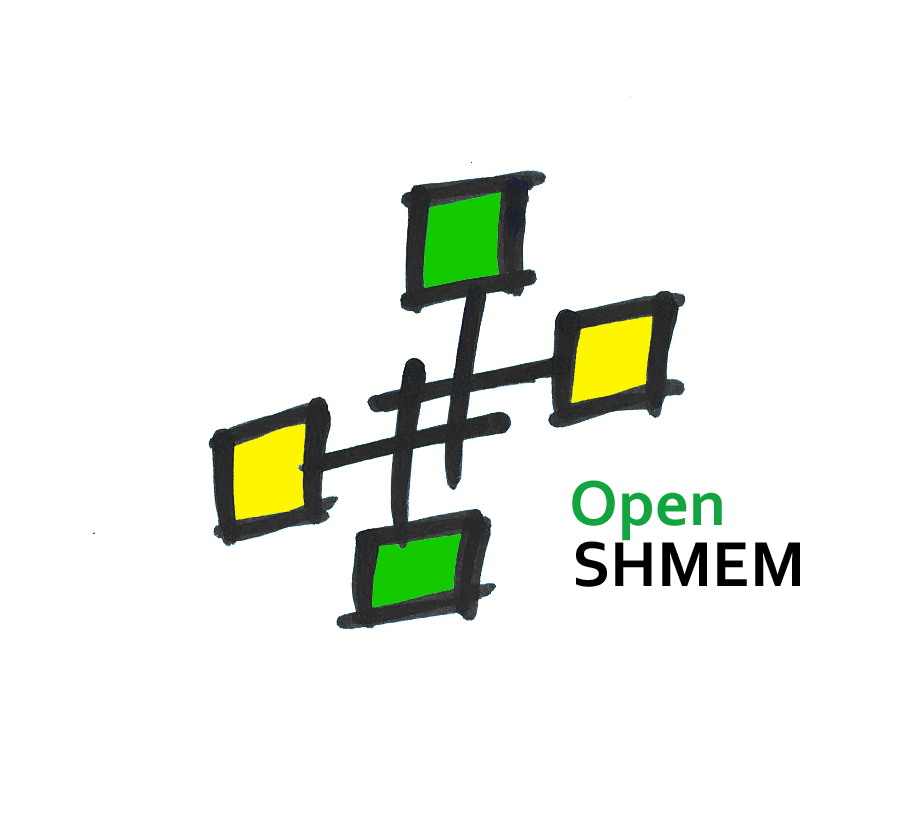
\includegraphics[scale=0.65]{figures/OpenSHMEM_Pound}\\
\url{http://www.openshmem.org/}
\par
\end{center}

\begin{center}
Version \insertDocVersion
\par
\end{center}

\vspace{0.5in}
\begin{center}
\today
\end{center}

\vspace{0.5in}

\vfill{}

\section*{Developed by}
\begin{itemize}
\item High Performance Computing Tools group at the University of Houston\\
  \url{http://www.cs.uh.edu/~hpctools/} 
\item Extreme Scale Systems Center, Oak Ridge National Laboratory\\
  \url{http://www.csm.ornl.gov/essc/} 
\end{itemize}
\pagebreak{}

\section*{Sponsored by}
\begin{itemize}
\item \ac{DoD}\\
  \url{http://www.defense.gov/ }
\item \ac{ORNL}\\
  \url{http://www.ornl.gov/} 
\end{itemize}

\section*{Authors and Collaborators}
\begin{itemize}
\item Monika ten Bruggencate
\item Matthew Baker, \ac{ORNL}
\item Barbara Chapman, \ac{UH} 
\item Tony Curtis, \ac{UH}
\item Eduardo D'Azevedo, \ac{ORNL}
\item James Dinan, Intel
\item Karl Feind, SGI
\item Manjunath Gorentla Venkata, \ac{ORNL}
\item Jeff Hammond, Intel
\item Oscar Hernandez, \ac{ORNL}
\item David Knaak, Cray Inc.
\item Gregory Koenig, \ac{ORNL}
\item Jeff Kuehn, \ac{LANL}
\item Graham Lopez, \ac{ORNL}
\item Jens Manser, \ac{DoD}
\item Tiffany M. Mintz, \ac{ORNL}
\item Nicholas Park, \ac{DoD}
\item Steve Poole, OSSS
\item Wendy Poole, OSSS
\item Swaroop Pophale, \ac{ORNL}
\item Michael Raymond, SGI
\item Pavel Shamis, \ac{ORNL}
\item Sameer Shende, \ac{UO}
\item Lauren Smith, \ac{DoD}
\item Aaron Welch, \ac{ORNL}

\end{itemize}

\date{\today}

\section*{Acknowledgements}
The \openshmem specification belongs to Open Source Software Solutions, Inc.
(OSSS), a non-profit organization, under an agreement with SGI. The development
work of the specification is supported by the Oak Ridge National Laboratory
Extreme Scale Systems Center and the Department of Defense.\\
\\
We would also like to acknowledge the contribution of the members of the
\openshmem mailing list for their ideas, discussions, suggestions, and
constructive criticism which has helped us improve this document.




\setcounter{tocdepth}{3}
\tableofcontents

\mainmatter  % included for use of documenttype 'book' 
\pagestyle{headings}  \withlinenumbers

\renewcommand{\thesection}{\arabic{section}} 
\startchap
\section*{Introduction}
\label{sec:intro}
%\section{Introduction}

This document defines the elements of the \openshmem  Application Programming
Interface~\footnote{SHMEM and \openshmem  are trademarks of Silicon Graphics International Corp.}.
The purpose of the \openshmem  API is to provide programmers
with a standard interface for writing parallel programs
using \Clang, \Cpp{} and \Fortran{} with one-sided communication.

More information about the \openshmem  project can be found at:\\
\url{http://www.openshmem.org/}

%\section{Overview}
\openshmem{} is a one-sided \ac{PGAS} library interface specification. In the \ac{PGAS} model, each process has local (or private) and 
globally shared memory that can be accessible by all processes where portions of the shared memory may have affinity to a particular process. 
\openshmem{} implements \ac{PGAS} using symmetric memory data objects to share information among processes or \ac{PE}s.   
\openshmem{} provides interfaces to perform communication and synchronization operations on both local and symmetric memory. 
\openshmem{} is a library and unlike UPC, CAF, Titanium, X10 and Chapel, which are all
PGAS languages, it relies on the programmer to create, destroy, access symmetric data objects, and synchronize \ac{PE}s using library calls.

The \openshmem specification is a result of effort to standardize widely available SHMEM implementations. 
The initial goal of the specification is to consolidate the existing vendor SHMEM implementations into a single specification, and  pave the way for 
a de-facto standard for SHMEM driven by the \openshmem community. A de-facto standard enables portability of SHMEM programs, and 
allows vendors to build and optimize their hardware architecture for OpenSHMEM.

The \openshmem{} specification defines library calls, constants, variables, and language bindings for \Clang{} and \Fortran{}.
Some of important \openshmem{} operations that you can do with \openshmem are as follows:

\begin{enumerate}
\item \textbf{Data Transfers }

\begin{enumerate}
\item One-sided puts : the initiator \ac{PE} (active side) specifies the local
data to be written to the target \ac{PE}'s (passive side) memory. 
\item One-sided gets : an explicit fetch operation is used to copy a variable
amount of data from a remote process and store it locally.\end{enumerate}
\begin{description}
\item [{{Note:}}] By avoiding the need for matching send and receive
calls, \openshmem simplifies the communication process by reducing the
number of calls required to have one \ac{PE} interact with other \ac{PE}s. 
\end{description}
\item \textbf{Synchronization Mechanisms }

\begin{enumerate}
\item Fence: Ensures ordering of PUT operations to a specific \ac{PE}. 
\item Quiet: Ensures ordering of PUT operations to all \ac{PE}s. 
\item Barrier: A collective synchronization routine in which no \ac{PE} may leave
the barrier prior to all \ac{PE}s entering the barrier. 
\end{enumerate}
\item \textbf{Collective Communication}

\begin{enumerate}
\item Broadcast: Copy a block of data from one \ac{PE} to one or more remote
PEs. 
\item Collection: Concatenate elements from the source array to a target
array over the specified \ac{PE}s. 
\item Reduction: Perform an associative binary operation over the specified
\ac{PE}s. 
\end{enumerate}
\item \textbf{Address Manipulation}

\begin{enumerate}
\item Allocating and deallocating memory blocks in the symmetric space.
\end{enumerate}
\item \textbf{Locks}

\begin{enumerate}
\item Implementation of mutual exclusion.
\end{enumerate}
\item \textbf{Atomic Memory Operations}

\begin{enumerate}
\item Swap, Conditional Swap, Add and Increment 
\end{enumerate}
\item \textbf{Data Cache control}

\begin{enumerate}
\item Implementation of mechanisms to exploit the capabilities of hardware
cache if available.
\end{enumerate}
\end{enumerate}
\begin{description}
\item [{{Note:}}] More information about \openshmem routines can be found
in the Library Routines section.
\end{description}


%
\section{What is \openshmem?}

This section is an introduction to previous work on \openshmem. We begin
with a quick overview of the Partitioned Global Address Space model,
which is the basis for \openshmem's data sharing strategy.


\subsection{Partitioned Global Address Space}

Conventional Parallel Programming Models can be broadly classified
into 2 types: 
\begin{description}
\item [{{Shared-Memory~Model:}}] in this model all processors interact
with a globally available memory space. 
\item [{{Distributed-Memory~Model:}}] in this model each processor has
its own memory to work with and can only directly access the data
that resides in its memory. When a processor needs data from another
processor an explicit function call must be made to communicate with
the target processor. 
\end{description}
The current high performance computing architectures prefer a combination
of the above mentioned memory models, which is referred to \textbf{Partitioned
Global Address Space} or PGAS for short. In PGAS, each processing
element (\ac{PE}) has access to its own private local memory and also to
a shared memory space. This programming model enhances performance
by exposing data/thread locality. PGAS programming languages include
\textbf{Unified Parallel \Clang (UPC)}, \textbf{Co-Array \Fortran (CAF)},
\textbf{Titanium}, \textbf{X-10} and \textbf{Chapel}.

More information about PGAS can be found at the PGAS Forum website.\cite{pgasfor}


\subsection{\openshmem}

% SGI asked for this to be removed to protect the trademark
%
%      SHMEM stands for \textbf{SH}ared \textbf{MEM}ory.

\openshmem is a library API that allows its participating processes (the
places where work occurs are called Processing Elements or \ac{PE}s) to
view a Partitioned Global Address Space. Each \ac{PE} is able to see
variables with a common name, but each \ac{PE} has its own local copy
of the variable.

The \openshmem library provides inter-processor communication using data
passing and one-sided communication techniques. \openshmem differs from
the Message Passing Interface (MPI), currently the most widely used
communication model, in that the latter generally uses two-sided communication
(MPI now also includes one-sided calls). In two-sided communication,
both sides of the exchange (source and destination) are required to
participate actively. The one-sided communication mechanism decouples
data transfer and synchronization, reducing communication overhead,
resulting in faster communication patterns. Figure \ref{fig:Communication-Scheme}
shows diagrams for one-sided and two-sided communications.\medskip{}


%\begin{center}
%\begin{figure}[H]
%\begin{centering}
%\includegraphics[scale=0.7]{media/communication} 
%\par\end{centering}
%
%\caption{Communication Scheme\label{fig:Communication-Scheme}}
%\end{figure}
%
%\par\end{center}

\medskip{}
The following are some of the communication operations available in
\openshmem:
\begin{enumerate}
\item \textbf{Data Transfers }

\begin{enumerate}
\item One-sided puts : the initiator \ac{PE} (active side) specifies the local
data to be written to the target \ac{PE}'s (passive side) memory. 
\item One-sided gets : an explicit fetch operation is used to copy a variable
amount of data from a remote process and store it locally.\end{enumerate}
\begin{description}
\item [{{Note:}}] By avoiding the need for matching send and receive
calls, \openshmem simplifies the communication process by reducing the
number of calls required to have one \ac{PE} interact with other \ac{PE}s. 
\end{description}
\item \textbf{Synchronization Mechanisms }

\begin{enumerate}
\item Fence: Ensures ordering of PUT operations to a specific \ac{PE}. 
\item Quiet: Ensures ordering of PUT operations to all \ac{PE}s. 
\item Barrier: A collective synchronization routine in which no \ac{PE} may leave
the barrier prior to all \ac{PE}s entering the barrier. 
\end{enumerate}
\item \textbf{Collective Communication}

\begin{enumerate}
\item Broadcast: Copy a block of data from one \ac{PE} to one or more target
\ac{PE}s. 
\item Collection: Concatenate elements from the source array to a target
array over the specified \ac{PE}s. 
\item Reduction: Perform an associative binary operation over the specified
\ac{PE}s. 
\end{enumerate}
\item \textbf{Address Manipulation}

\begin{enumerate}
\item Allocating and deallocating memory blocks in the symmetric space.
\end{enumerate}
\item \textbf{Locks}

\begin{enumerate}
\item Implementation of mutual exclusion.
\end{enumerate}
\item \textbf{Atomic Memory Operations}

\begin{enumerate}
\item Swap, Conditional Swap, Add and Increment 
\end{enumerate}
\item \textbf{Data Cache control}

\begin{enumerate}
\item Implementation of mechanisms to exploit the capabilities of hardware
cache if available.
\end{enumerate}
\end{enumerate}
\begin{description}
\item [{{Note:}}] More information about \openshmem routines can be found
in the Library Routines section.
\end{description}

\subsection{History of \openshmem}
\begin{description}
\item [{{Cray~SHMEM~(MP-SHMEM,~LC-SHMEM):}}] Cray first introduced
SHMEM in 1993 for its Cray T3D systems. Cray SHMEM was also used in
other models: T3E, PVP and XT series. 
\item [{{SGI~SHMEM~(SGI-SHMEM):}}] Cray Research merged with Silicon
Graphics (SGI) in February 1996. At this point SHMEM was incorporated
into SGI's Message Passing Toolkit (MPT). The platforms supported
were - SGI Irix, Origin and Altix. 
\item [{{Quadrics~SHMEM~(Q-SHMEM):}}] an optimized API for the Quadrics
QsNet interconnect. It included SGI extensions and provided non-blocking
puts and gets. A joint effort from HCS Lab \& Quadrics incorporated
a program profiling interface called PSHMEM that can aid in the execution
analysis of SHMEM programs. 
\end{description}
The success of SHMEM's performance attracted several vendors to provide
implementations (with varying names and features) for their systems.
Some of them include: 
\begin{description}
\item [{{HP~SHMEM:}}] Based on the Quadrics API. It is included in the
UPC product kit. 
\item [{{Cyclops-64~SHMEM~(C64-SHMEM):}}] this SHMEM API supports the
Cyclops-64 architecture. Most of the core features of Cray SHMEM are
available with some additional interfaces specific to the Cyclops-64
architecture. %
%\begin{comment}
%Forcing new line, can't get \LaTeX{} to do it automatically.
%\end{comment}

\item [{{IBM~SHMEM:}}] An implementation created by IBM intended for
internal use only. 
\item [{{TurboSHMEM:}}] This implementation uses IBM's Low-Level API
(LAPI) technology to obtain optimized one-sided communication for
the put/get operations. This allows applications written with the
SHMEM API to run on IBM platforms with minimal source code changes. 
\item [{{GPSHMEM:}}] This implementation of SHMEM aims at providing full
portability of applications. It is built mostly with Cray T3D components
and functionalities and provides MPI and ARMCI support. This project
is no longer maintained. \end{description}


\section{The \openshmem Effort}

\openshmem is a SHMEM specification that aims at consolidating the different
SHMEM versions provided by vendors, laboratories and universities 
into a single widely accepted specification. \openshmem addresses the
current and future SHMEM community needs in a single specification. Vendors are starting to provide \openshmem implementations to help the user
write portable \openshmem code that can run on multiple platforms  so that they don't have to deal with the
subtle differences that come from vendor-specific implementations. For more details on the history of 
the \openshmem please refer to \hyperref[sec:openshmem_history]{The History of \openshmem section}.  

The \openshmem effort is driven by the \ac{ESSC} at \ac{ORNL} and the \ac{UH} 
with significant input from the \openshmem{} community. Besides the
specification, the effort includes providing a reference implementation,
and building infrastructure for the defacto standardization process.
The specifications and the reference implementations are available here: 
www.openshmem.org. 

%\rcomment{Manju: 1) We are introducing \openshmem{} without describing what it
%is. 2) Second paragraph, IMO, this gives a impression that \openshmem{} effort is all about
%consolodiation. Rather, it should be that only 1.0 and 1.1 have this aim. 
%Future version is not aimed at consolodition. How does these two paragraphs 
%look ?}
%\rcomment{ \\ Oscar: 1) OpenSHMEM does not provide a global view of memory that is addressable by all PEs (like UPC, Chapel, where there is a PGAS address space). Instead
%it provides partioned-view of data, where symmetric data objects are accessible by all PEs. We need to avoid saying that OpenSHMEM provides a shared addressable space. 
%}
%
%\openshmem is a \ac{PGAS} library interface specification. In the \ac{PGAS} model, each process has access to 
%local private and globally shared memory, where portions of the shared memory may have affinity to a particular process. \openshmem
%defines interfaces for implementing a \ac{PGAS} program 111 access symmetric data objects ,  communication and synchronization on the address space. 
%
%\rcomment{Oscar: 2 OpenSHMEM I'm not sure if a spec can be defined as open source}
%\openshmem is the first community-driven SHMEM specification,
%which is a consolidation of various SHMEM specifications that addresses SHMEM community needs. 
%One of the goals of \openshmem is to consolidate different SHMEM versions
%provided by the vendors, laboratories, and universities into a single open
%source specification. In the past, different SHMEM implementations have a subtle
%differences, and as a consequence, SHMEM programs written using any one of these 
%implementations was portable across systems. 
%More details on the history of the \openshmem are available in this
%\hyperref[sec:openshmem_history]{section}.
%
%The \openshmem standardization effort is driven by \ac{ORNL} and \ac{UH} 
%with significant input from the \openshmem{} community. Besides the
%specification, the effort included providing a reference implementation,
% and building infrastructure for the standardization process.
%The specifications and the reference implementations are available here: 
%www.openshmem.org.
%
%\rcomment{Manju: Do we have to add a paragraph about the role of OSS ?}
%\rcomment{Probably not, up-to Steve} 

\label{subsec:osh_project}
\section{Programming Model Overview}
%SP: Addressing suggestions from discussion on 01/28/2014 Merging the commented portions into the body. 
%The \openshmem programming model consists of library functions that provide
%low-latency, high-bandwidth communication  for  use  in  highly  parallelized 
%scalable programs. The functions in the \openshmem \ac{API} provide a programming 
%model for exchanfging data between cooperating parallel processes. The resulting programs are similar 
%in style to \ac{MPI} programs. The \openshmem \ac{API} can be used either alone 
%or in combination with \ac{MPI} functions in the same parallel program.
%\openshmem implements a \ac{PGAS} model. 
%In the \ac{PGAS} model, each process has a local and globally shared memory where portions of the shared memory may have affinity to a particular process. 
\openshmem implements \ac{PGAS} by defining remotely accessible data objects as a mechanism to share information among \openshmem processes or \acp{PE} and private data objects that are accessible by the \ac{PE} 
itself. The \ac{API} allows communication and synchronization operations on both private (local) and remotely accessible data objects. The key feature of \openshmem is that data transfer functions are \textit{\textbf{one-sided}} in nature. This means that a local \ac{PE} executing a data transfer does not require the participation of the remote \ac{PE} to complete the operation. This allows for overlap between communication and computation to hide data transfer latencies, which makes  \openshmem ideal for unstructured, small/medium size data communication patterns. The \openshmem library functions have the potential to provide low-latency, high-bandwidth communication \ac{API} for use in highly parallelized scalable programs. 

%\rcomment{Manju: To do - Make sure the first paragraph does not say the same
%things has first paragraph of Section 1}

%An \openshmem program is currently \ac{SPMD} in style. The
%\openshmem  processes, called \ac{PE}s, all start at the
%same time, and they all run the same program. Usually the \ac{PE}s perform
%computation on their own subdomains of the larger problem, and periodically 
%communicate with other \ac{PE}s to exchange information on which the
%next computation phase depends.
%SP: Addressing suggestions from discussion on 01/31/2014

%Data latency is  the  period  of  time that starts when a \ac{PE} initiates a transfer of data 
%and ends when a \ac{PE} can use the data. %SP: What about put? Not guaranteed till synchronization is hit.

%SP: Addressing suggestions from discussion on 01/28/2014
%\openshmem functions support remote data transfer through \FUNC{put} operations, which  transfer data to a 
%different \ac{PE}, get operations, which transfer data from a different \ac{PE}, and remote pointers, which 
%allow direct  references  to  data objects owned by another \ac{PE}. Other operations supported are \FUNC{collective} 
%\FUNC{broadcast} and \FUNC{reduction}, \FUNC{barrier synchronization}, and \FUNC{atomic memory operations}. 
%An atomic memory operation  is an atomic read-and-update operation, such as a fetch-and-increment, on a remote
%or local data object.

%\rcomment{Manju: [The idea is to talk SPMD. We are talking about nature of interfaces rather than 
% the interfaces that enable SPMD. Replace the second paragraph with the one below ?]}
%\rcomment{\\ Oscar: I'm good with this change. minor change to say the SPMD can be used to decompose work\\}
The \openshmem{} interfaces can be used to implement \ac{SPMD} style programs. It provides interfaces 
to start the \openshmem{} \ac{PE}s in parallel, and communication and synchronization interfaces to access remotely accessible data objects across \ac{PE}s. These interfaces can be leveraged to divide a problem into multiple sub-problems that can solved independently or with coordination using the communication and synchronization interfaces.
The \openshmem specification defines library calls, constants, variables, and language bindings for \Clang{} and \Fortran{}.
The \Cpp{} interface is currently the same as that for \Clang. Unlike UPC, Fortran 2008, Titanium, X10 and Chapel, which are all PGAS languages, \openshmem relies on 
the programmer to use the library calls  to implement the correct semantics of its programming model.

An overview of the important \openshmem operations is described below:

\begin{enumerate}
\item \textbf{One-sided Data Transfers }

\begin{enumerate}
\item \FUNC{Put}: The local \ac{PE} specifies the source
data (local or symmetric) that is copied to the symmetric data object on the remote \ac{PE}. 
\item \FUNC{Get}: The local \ac{PE} specifies the symmetric data object on the remote \ac{PE}
that is copied to a data object (local or symmetric) on the local \ac{PE}. 
\end{enumerate}

\item \textbf{Synchronization Mechanisms }
\begin{enumerate}
\item \FUNC{Fence}: The \ac{PE} calling fence ensure ordering of \FUNC{Put} operations with respect to a specific target \ac{PE}. 
\item \FUNC{Quiet}: The \ac{PE} calling quiet ensures ordering of \FUNC{Put} operations before the next local or remote update. 
\item \FUNC{Barrier}: All or some \ac{PE}s collectively synchronize and ensure completion of remote and local updates prior to any \ac{PE} returning from the call.
\end{enumerate}
\item \textbf{Collective Communication}

\begin{enumerate}
\item \FUNC{Broadcast}: The \textit{root} \ac{PE} specifics a symmetric data object to be copied to a symmetric data object on one or more remote \ac{PE}s (not including itself). 
\item \FUNC{Collection}: All \ac{PE}s participating in the operation get the result of concatenated symmetric objects contributed by each of the \ac{PE} in another symmetric data object.
\item \FUNC{Reduction}: All \ac{PE}s participating in the operation get the result of associative binary operation over elements of the specified symmetric data object on another symmetric data object. 
\end{enumerate}

\item \textbf{Managing symmetric data objects}
\begin{enumerate}
\item \FUNC{Allocation}: All executing \ac{PE}s must participate in the allocation of a symmetric data object with identical arguments.
\item  \FUNC{Deallocation}: All executing \ac{PE}s must participate in the deallocation of the same symmetric data object with identical arguments.
\item  \FUNC{Reallocation}: All executing \ac{PE}s must participate in the reallocation of the same symmetric data object with identical arguments.
\end{enumerate}

\item \textbf{Mutual Exclusion}
\begin{enumerate}
\item \FUNC{Set Lock}: The \ac{PE} acquires exclusive access to the region bounded by the symmetric \textit{lock} variable.
\item \FUNC{Test Lock}: The \ac{PE} tests the symmetric \textit{lock} variable for availability.
\item \FUNC{Clear Lock}: The \ac{PE} which has previously acquired the \textit{lock} releases it.
\end{enumerate}

\item \textbf{Atomic Memory Operations}
\begin{enumerate}
\item \FUNC{Swaps}: The \ac{PE} initiating the swap gets the old value of the symmetric data object it is copying a new value to on the remote \ac{PE}.
\item \FUNC{Increments}: The \ac{PE} initiating the increment adds 1 to the symmetric data object on the remote \ac{PE}.
\item \FUNC{Add}: The \ac{PE} initiating the add specifics the value to be added to the symmetric data object on the remote \ac{PE}.
\end{enumerate}

\item \textbf{Data Cache control \textit{(deprecated)}}
\begin{enumerate}
\item Implementation of mechanisms to exploit the capabilities of hardware
cache if available.
\end{enumerate}
\end{enumerate}

%\begin{description}
%\item [{{Note:}}] More information about \openshmem routines can be found
%in the Library Routines section.
%\end{description}

\label{subsec:programming_model}
%Outline
%%Exectution model
%   *Define what is a OpenSHMEM program: a set of processes (either SPMD or MIMD?) where each process has its own 'local' (private) memory and symmetric memory regions that may be accessible by any PEs.
%   *Each OpenSHMEM process is called a processing element (PE)
%   *Each PE may be mapped to many to one hardware cores/threads or less.
%   *The number of PEs is specified at launch/runtime.
%   *Each PE must call startpe to initialize the OpenSHMEM runtime, before any other call for OpenSHMEM. There is an implicit barrier at startpe.
%   *Each PE executes asynchronously following Fortran or program execution in C [ISO/IEC00 Sec. 5.1.2.3]
%   *Each PE will have a unique global identifier and the execution of a program may depend on the PE id, if executed in SPMD.
%   *PE id may be used for library calls synchronizations, control flow constructs language  in C/Fortran
%   *PE may allocate symmetric data objects via a symmetric heap 
%   *As of now, PEs may finish execution at any time by returning from the main function. (no call to shmem_finalize yet!)
%   
%  %Memory model
%    *Each OpenSHMEM PEs may have symmetric memory that is accessible by other PEs. 
%    *Symmetric memory is a region of memory where all the an instance of a data objects is replicated across PEs, have 
%     the same the same layout and relative offset.
%    *All PEs can allocate a symmetric data objects using the symmetric heap, but they must do so as a collective operation. (is there a barrier after shmalloc?)
%    *All writes to symmetric memory are relaxed (I'm not sure if this is the completion semantics) and are guaranteed to be visible to other PEs after a barrier_all, barrier(?), quiet, (what about wait? does it means iti sonly visible to me?) 
%    *Calls to barrier, barrier_all, quiet, wait, lock, atomics, are meant to guarantee memory consistency across PEs.
%    *Read/Writes to symmetic data object may appear after startpe or after a the symmetric data object has been allocated in the symmetric heap (if it is a dynamic).
%    *Operations like reduction, collect, etc guarantee memory consistency after completion(?)
%    *Data races are possible in OpenSHMEM if multiple PEs write/read a symmetric data object from a single PE without proper synchronization.  
%
%This comes from the UPC spec:
%The memory consistency model in a language defines the order in which the results of write operations may be observed through read operations.
%The behavior of a OpenSHMEM program may depend on the timing of accesses to symetric variables on PEs, so in general a program defines a set of possible executions, 
%rather than a single execution. The memory consistency model constrains the set of possible executions for a given program; the user may then rely 
%on properties that are true of all of those executions.

\section{Memory Model}
\begin{figure}[h]
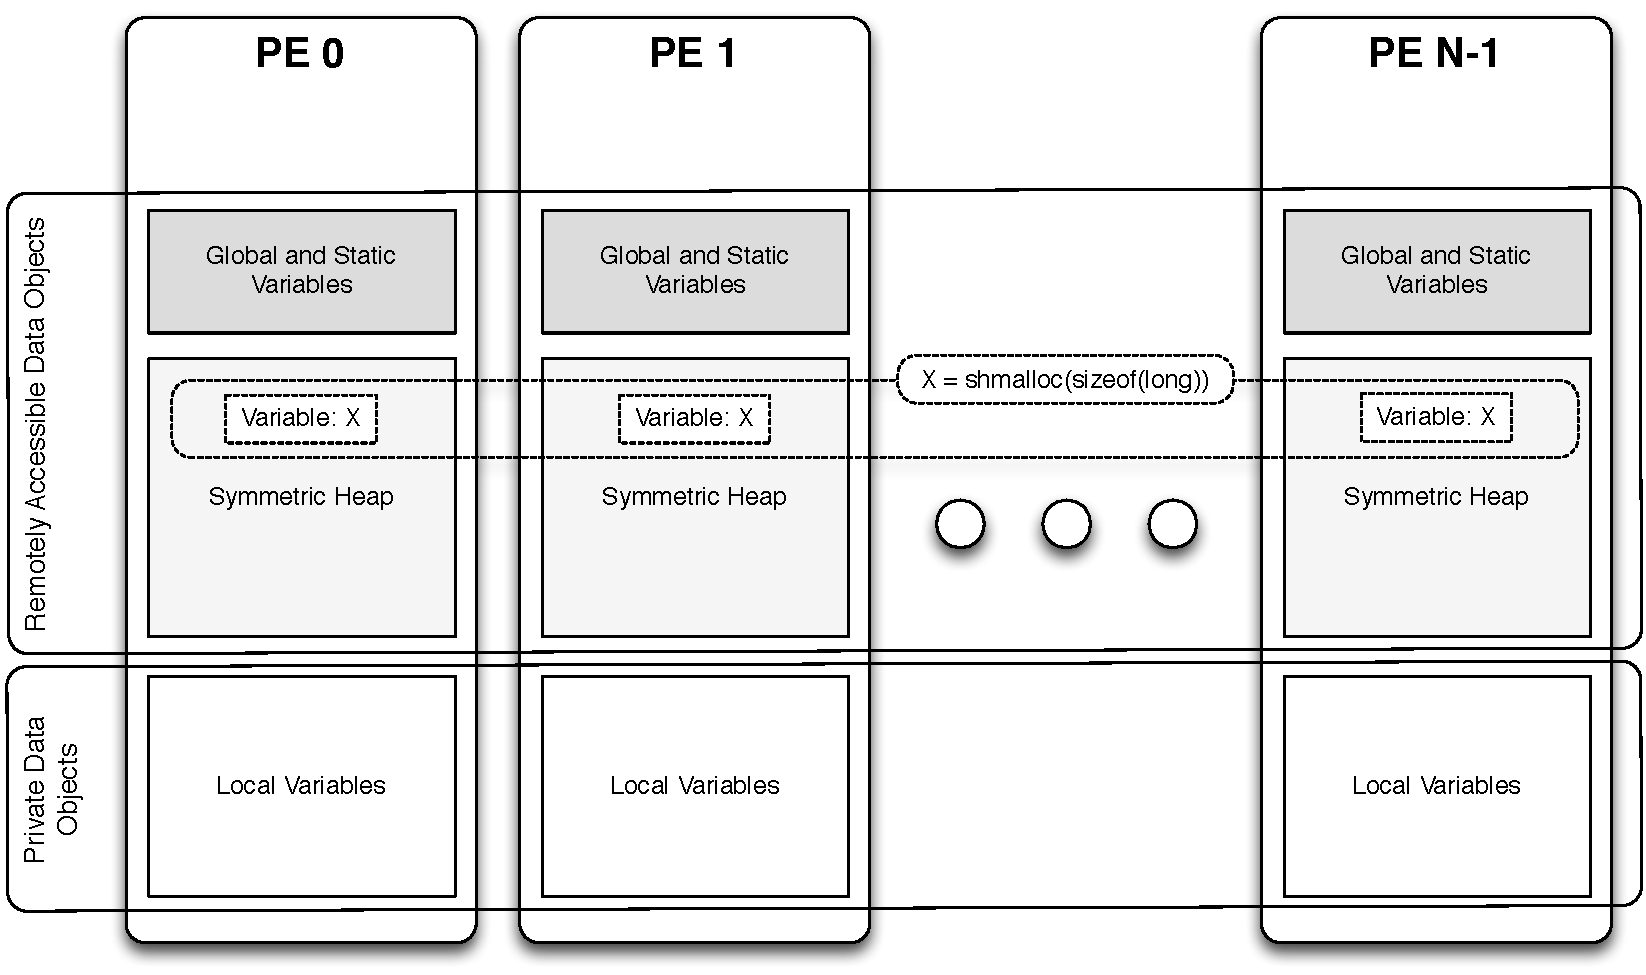
\includegraphics[width=0.95\textwidth]{diagrams/updated/mem_model}      
\caption{\OSH{} Memory Model}                                   
\label{fig:mem_model}                                               
\end{figure}      
An \openshmem program consists of data objects that are private to each \ac{PE} and data 
objects that are remotely accessible by all \ac{PE}s. Private data objects are stored in the local
memory of each \ac{PE} and can only be accessed by the \ac{PE} itself; these data objects
cannot be accessed by other \ac{PE}s via \openshmem routines. Private data objects
follow the memory model of \Clang{} or \Fortran{}. Remotely accessible
objects, however, can be accessed by remote \ac{PE}s using \openshmem routines.
Remotely accessible data objects are called \emph{Symmetric Objects}.
%An object is symmetric if it has a corresponding object with the same   
%SP: No, if there is a way to create such objects without them being global/static/common/save or shmalloced/shpalloced would they would be symmetric as per this definition...NOT the way OpenSHMEM defines.
All symmetric data objects have a corresponding object with the same
name, type, size, and offset (from an arbitrary memory address) on all \ac{PE}s. \emph{Symmetric objects } are accessible by all executing \ac{PE}s via the \openshmem \ac{API}.  
In \openshmem{} the following kinds of data objects are symmetric:
\begin{itemize}
  \item \Fortran{} data objects in common blocks or with the  SAVE  attribute. These data objects must not be defined in a dynamic shared object (DSO).
  \item Non-stack \Clang{} and \Cpp{} variables.   These  data	objects must  not  be defined in a DSO.
  \item \Fortran{} arrays allocated with \textit{shpalloc} 
  \item \Clang{} and \Cpp{} data allocated by \textit{shmalloc}
\end{itemize}       

%Symmetric Objects
%are static and global variables in \Clang{} and \Cpp, which are often allocated
%at the same address on all \ac{PE}s where the program is being executed
%(\emph{e.g.} in the ELF executable format). 
%See Figure \ref{fig:SymmetricHeap1}
%for an example of how Symmetric Memory Objects may be arranged in
%memory.
\openshmem dynamic memory allocation routines (\textit{shpalloc} and \textit{shmalloc}) allow collective allocation of \emph{Symmetric
Data Objects} on a special memory region called the Symmetric Heap. The Symmetric Heap is created during the execution of a program at a memory location
determined by the implementation. The Symmetric Heap may reside on different memory regions on different \ac{PE}s. Figure~\ref{fig:mem_model} shows how \openshmem implements a \ac{PGAS} model using remotely accessible (\emph{Symmetric objects}) and private data objects when executing a \Clang{} or \Fortran program. Symmetric data objects are stored on the symmetric heap or 
in the global / static memory section of each \ac{PE}. 

%Symmetric data objects can be allocated dynamically in the symmetric heap of each \ac{PE} using
%a collective \FUNC{shmalloc} or \FUNC{shpalloc} memory allocation call.
     
%\openshmem specification does not require a particular memory layout; it is up to the implementation
%to decide how to implement the symmetric heap.  
%Objects that reside in the private address space can only be accessed by the \ac{PE} itself; these data objects
%cannot be accessed by other \ac{PE}s via \openshmem routines. 

\label{subsec:memory_model}
%%Outline
%%Exectution model
%   *Define what is a OpenSHMEM program: a set of processes (either SPMD or MIMD?) where each process has its own 'local' (private) memory and symmetric memory regions that may be accessible by any PEs.
%   *Each OpenSHMEM process is called a processing element (PE)
%   *Each PE may be mapped to many to one hardware cores/threads or less.
%   *The number of PEs is specified at launch/runtime.
%   *Each PE must call startpe to initialize the OpenSHMEM runtime, before any other call for OpenSHMEM. There is an implicit barrier at startpe.
%   *Each PE executes asynchronously following Fortran or program execution in C [ISO/IEC00 Sec. 5.1.2.3]
%   *Each PE will have a unique global identifier and the execution of a program may depend on the PE id, if executed in SPMD.
%   *PE id may be used for library calls synchronizations, control flow constructs language  in C/Fortran
%   *PE may allocate symmetric data objects via a symmetric heap  during execution%SP: Does not cover global and static.
%   *As of now, PEs may finish execution at any time by returning from the main routine. (no call to shmem_finalize yet!)
%   
%This comes from the UPC spec:
%The memory consistency model in a language defines the order in which the results of write operations may be observed through read operations.
%The behavior of a OpenSHMEM program may depend on the timing of accesses to symmetric variables on PEs, so in general a program defines a set of possible executions, 
%rather than a single execution. The memory consistency model constrains the set of possible executions for a given program; the user may then rely 
%on properties that are true of all of those executions.
    

\section{Execution Model}
%\openshmem  can use a single process multiple data (SPMD) or MIMD 
%parallelism.  An \openshmem application makes use of multiple processors,
%referred to as Processing Elements or PEs, to complete operations
%in parallel. 
Although \openshmem follows the SPMD execution model, different \ac{PE}s may have different execution paths and will execute asynchronously following \Fortran{} or program execution in \Clang.  Each \ac{PE} may be mapped to many to one hardware cores/threads or less. In \openshmem the number of \ac{PE}s is specified at runtime.

\openshmem requires initialization before using any of the \openshmem library
routines by calling \textbf{start\_pes()}.  %during the initialization phase of a program. %SP:repetitive.
The \ac{PE}s do not exist till after \FUNC{start\_pes} returns. \FUNC{start\_pes} performs any required initialization steps, such as setting up the symmetric heap for every \ac{PE} and creating and assigning \ac{PE} numbers which act like unique global identifiers for the duration of the program. These \ac{PE} identifiers are integers assigned in a monotonically increasing manner from zero to the total number of \ac{PE}s minus 1. \ac{PE} identifiers are used on \openshmem library calls (i.e. to access symmetric objects from specific \ac{PE}s, collective synchronization, etc.) or to dictate a definite control flow for \ac{PE}s using constructs of \Clang{} or \Fortran. Some collective routines require the creation of an \activeset, which is  group of \ac{PE}s that is involved in the execution of a collective routine. These collective routines assume that only \ac{PE}s in the \activeset{} call the routine. If a \ac{PE} not in the \activeset{} calls an \openshmem collective routine, undefined  behavior results.
An OpenSHMEM program consists of a set of processes, called \ac{PE}s where each process has its own 'local' (private) memory and symmetric memory regions that may be accessible by any \ac{PE}s.
Although \openshmem follows the \ac{SPMD} execution model, different \ac{PE}s may have different execution paths and will execute asynchronously following \Fortran{} or program execution in \Clang{} or \Cpp.  Each PE may be mapped to many to one hardware cores/threads or less. In \openshmem the number of \ac{PE}s is specified at runtime.

\openshmem requires initialization before using any of the OpenSHMEM library
routines by calling \FUNC{start\_pes}.%during the initialization phase of a program. %SP:repetitive.
The \ac{PE}s do not exist till after \FUNC{start\_pes} returns. \FUNC{start\_pes} performs any required initialization steps, such as setting up the symmetric heap for every \ac{PE} and creating and assigning \ac{PE} numbers 
which act like unique global identifiers for the duration of the program. These \ac{PE} identifiers are integers assigned in a monotonically increasing manner from zero to the total number of \ac{PE}s minus 1. \ac{PE} identifiers 
are used for other \openshmem library calls (such as collective synchronization) or to dictate a definite control flow for \ac{PE}s using constructs of \Clang{} or \Fortran{}. Some collective routines require the creation of an 
\activeset, which is  group of \ac{PE}s that is involved in the execution of a collective routine. These collective routines assume that only \ac{PE}s in the \activeset{} call the routine. If a \ac{PE} not in the \activeset{} calls a 
\openshmem collective routine, undefined  behavior results.

%The symmetric heap is one of the memory spaces
%that is remotely accessible by all PEs. The symmetric heap is discussed
%further in the Memory Model section. The PE numbers are the
%identifiers used to refer to each of the PEs involved in the execution.
%Consistent with the SPMD nature of the \openshmem programming model  is  the concept of symmetric data objects.  These are arrays or variables that exist with the same size,  type,	 and  relative	address	 on  all  PEs. Another	term  for  symmetric data objects is "remotely accessible data objects."  In the interface definitions for \openshmem data  transfer	 functions,  one or more of the parameters are typically required to be symmetric or remotely accessible. The following kinds of data objects are symmetric:
%\begin{itemize}
%  \item Fortran data objects in common blocks or with the  SAVE  attribute. These data objects	must not be defined in a dynamic shared object (DSO).
%  \item Non-stack C and C++ variables.   These  data	objects must  not  be defined in a DSO.
%  \item Fortran arrays allocated with \textit{shpalloc} 
%  \item C and C++ data allocated by \textit{shmalloc}
%\end{itemize}       
%
%Data transfer in \openshmem is possible through several one-sided put
%(for write) and get (for read) operations, as well as various collective
%routines such as broadcasts and reductions. Since the library provides the flexibility of one-sided operations the execution pattern is depends on the how the programmer decides to distribute work amongst different PEs and the synchronization and ordering operations used.
%
%Query routines are available to gather information about the execution.
%\openshmem also provides synchronization routines to coordinate data
%transfers and other operations. 
As of now, an \openshmem program finishes execution by returning from the main routine. 
It is up to the implementation on how to handle the finalization of the
\openshmem library and any other resources initialized by the library:
there is currently no explicit call defined in the \openshmem specification.


\subsection{Progress of \openshmem Routines}

The \openshmem model assumes that computation and communication are
naturally overlapped.  High quality \openshmem implementations must insure that programs exhibit %SP: Changing MUST to may as per discussion on 01/31/2014
progression of communication both with and without \openshmem calls.
Consider a \ac{PE} that is engaged in a long computation with no \openshmem calls.
Other \ac{PE}s must be able to communicate (put/get,
collective, atomic) with that computationally-bound \ac{PE} without that \ac{PE}
issuing any explicit \openshmem calls. \openshmem communication calls involving that \ac{PE} must progress
regardless of when that \ac{PE} next engages in an \openshmem call.

\textbf{Note to implementers:} progress will often be ensured through
the use of a dedicated progress thread in software, or through
network hardware that offloads communication handling from processors.

%\subsection{Using the Symmetric \VAR{Work} and \VAR{pSync} Arrays}

%Multiple \VAR{pSync} arrays are often needed if a particular \ac{PE} calls a \openshmem
%collective  function twice without intervening barrier synchronization.
%Problems would occur if some \ac{PE}s in the \activeset{} for call 2 arrive at
%call 2 before processing of call 1 is complete by all \ac{PE}s in the call 1
%\activeset.  You can use  \FUNC{shmem\_barrier}  or  \FUNC{shmem\_barrier\_all}  to
%perform  a  barrier  synchronization between consecutive calls to \openshmem
%collective functions. There are two special cases:
%\begin{itemize}
%\item The \FUNC{shmem\_barrier} function allows the same \VAR{pSync} array to be used
%          on consecutive calls as long as the active \ac{PE} set does not change.
%\item  If the same collective function is called multiple times with the
%          same \activeset, the calls may alternate between two \VAR{pSync} arrays.
%          The \openshmem functions guarantee that a first call is completely finished by 
%          all \ac{PE}s by the time processing of a third  call  begins  on
%          any \ac{PE}.          
%\end{itemize}
%Because  the \openshmem functions restore \VAR{pSync} to its original contents,
%multiple calls that use the same \VAR{pSync} array do not require that \VAR{pSync}
%be reinitialized after the first call.

\subsection{Atomicity Guarantees}

\openshmem contains a number of routines that operate on symmetric data
atomically.  These routines guarantee that accesses by \openshmem's
atomic routines will be exclusive, but do not guarantee exclusivity
in combination with other routines, either inside \openshmem or
outside.

For example: during the execution of a remote integer increment
routine on a symmetric variable \VAR{x}, no other \openshmem atomic
routine may access \VAR{x}.  After the increment, \VAR{x} will have
increased its value by \CONST{1} on the target \ac{PE}, at which point other
atomic routines may then modify that \VAR{x}.

%  %Memory model
%    *Each OpenSHMEM PEs may have symmetric memory that is accessible by other PEs. 
%    *Symmetric memory is a region of memory where all the an instance of a data objects is replicated across PEs, have 
%     the same the same layout and relative offset.
%    *All PEs can allocate a symmetric data objects using the symmetric heap, but they must do so as a collective operation. (is there a barrier after shmalloc?)
%    *All writes to symmetric memory are relaxed (I'm not sure if this is the completion semantics) and are guaranteed to be visible to other PEs after a barrier_all, barrier(?), quiet, (what about wait? does it means iti sonly visible to me?) 
%    *Calls to barrier, barrier_all, quiet, wait, lock, atomics, are meant to guarantee memory consistency across PEs.
%    *Read/Writes to symmetric data object may appear after startpe or after a the symmetric data object has been allocated in the symmetric heap (if it is a dynamic).
%    *Operations like reduction, collect, etc guarantee memory consistency after completion(?)
%    *Data races are possible in OpenSHMEM if multiple PEs write/read a symmetric data object from a single PE without proper synchronization.  

%Outline
%%Exectution model
%   *Define what is a OpenSHMEM program: a set of processes (either SPMD or MIMD?) where each process has its own 'local' (private) memory and symmetric memory regions that may be accessible by any PEs.
%   *Each OpenSHMEM process is called a processing element (PE)
%   *Each PE may be mapped to many to one hardware cores/threads or less.
%   *The number of PEs is specified at launch/runtime.
%   *Each PE must call startpe to initialize the OpenSHMEM runtime, before any other call for OpenSHMEM. There is an implicit barrier at startpe.
%   *Each PE executes asynchronously following Fortran or program execution in C [ISO/IEC00 Sec. 5.1.2.3]
%   *Each PE will have a unique global identifier and the execution of a program may depend on the PE id, if executed in SPMD.
%   *PE id may be used for library calls synchronizations, control flow constructs language  in C/Fortran
%   *PE may allocate symmetric data objects via a symmetric heap  during execution%SP: Does not cover global and static.
%   *As of now, PEs may finish execution at any time by returning from the main function. (no call to shmem_finalize yet!)
%   
%This comes from the UPC spec:
%The memory consistency model in a language defines the order in which the results of write operations may be observed through read operations.
%The behavior of a OpenSHMEM program may depend on the timing of accesses to symetric variables on PEs, so in general a program defines a set of possible executions, 
%rather than a single execution. The memory consistency model constrains the set of possible executions for a given program; the user may then rely 
%on properties that are true of all of those executions.
    

\section{Execution Model}
\label{subsec:execution_model}
%An \openshmem{} program consists of a set of processes, called \ac{PE}s, that execute in a \ac{SPMD}-like execution model. In \openshmem different \ac{PE}s can have different execution paths and will execute asynchronously 
%following \Fortran{} or \Clang{} program execution. The \ac{PE}s progress independently, and can communicate and synchronize using the \openshmem{} \ac{API}.
%The number of \ac{PE}s in the \openshmem{} program is specified at runtime by the user. %A \ac{PE} can be implemented as an OS process or OS thread~\footnote{As long as the memory model and execution model of \openshmem is followed.}. 
%The total number of \ac{PE}s, \VAR{N}, can be mapped to \VAR{M} hardware cores/threads where \VAR{M} can be less or equal than \VAR{N}. %As long as the memory model and execution model of \openshmem is followed.
%An \openshmem program must start by calling the initialization function \FUNC{start\_pes}  before using any of the other \openshmem library routines. \ac{PE}s do not exist until after the call to \FUNC{start\_pes} returns. 
%During execution, each \ac{PE} is assigned a unique global identifier for the duration of the program. These \ac{PE} identifiers are integers assigned in a monotonically increasing manner from zero to the total number of \ac{PE}s minus 1. \ac{PE} identifiers are used for other \openshmem library calls (e.g. to access symmetric objects from specific \ac{PE}s, collective synchronization) or to dictate a control flow for \ac{PE}s using constructs of 
%\Clang{} or \Fortran.  As of now, an \openshmem program finishes execution by returning from the main function. It is up to the implementation on how to handle the finalization of the \openshmem library and any other 
%resources initialized by the library: there is currently no explicit finalization call defined in the \openshmem specification.

An \openshmem{} program consists of a set of \openshmem{} processes called \ac{PE}s that execute in a \ac{SPMD}-like model where each \ac{PE} can take a different execution path. A \ac{PE} can be implemented using an OS process or an OS thread\footnote{Implementing \ac{PE}s using OS threads requires compiler techniques to implement the \openshmem{} memory model.}.  The \ac{PE}s progress asynchronously, and can communicate/synchronize 
via the \openshmem{} interfaces. All \ac{PE}s in an \openshmem{} program should start by calling the initialization routine  \FUNC{shmem\_init()} \footnote{\textbf{start\_pes()} has been deprecated as of Specification 1.2} before using any of the other \openshmem{} library routines. 
%SP: Spec 1.2, ticket 108, text from Oscar.
%As of now, an \openshmem program finishes execution by returning from the main function. On program exit, \openshmem must complete all pending communication and release all the resources associated to the library using an implicit collective synchronization across \ac{PE}s.
%On program exit, \openshmem can release all the resources associated to the library. 
%  It is up to the implementation on how to handle the finalization of the \openshmem library. 
An \openshmem program finishes execution by returning from the main routine or when any PE calls \FUNC{shmem\_global\_exit}. When returning from main, \openshmem must complete all pending communication and release all the resources associated to the library using an implicit collective synchronization across PEs. The
user has the option to call \FUNC{shmem\_finalize} (before returning from main) to complete all pending communication and release all the \openshmem library resources without terminating the program. Calling any \openshmem routine after \FUNC{shmem\_finalize} leads to undefined behavior.

The \ac{PE}{}s of the \openshmem{} program are identified by unique integers. The identifiers are integers assigned in a monotonically increasing manner from zero to the total number of \ac{PE}s minus 1. \ac{PE} identifiers are used for \openshmem{} calls (e.g. to specify \PUT{} or \GET{} routines on symmetric data objects, collective synchronization calls, etc.) or to dictate a control flow for \ac{PE}s using constructs of \Clang{} or \Fortran. The identifiers are fixed for the life cycle of the \openshmem{} program.
%on exit implementation are expected to release resources associated to the library
  %following \Fortran{} or \Clang{} program execution.
%Each \ac{PE} can be implemented as an OS process or OS thread as long as the constraints imposed
%by the memory model and execution model are respected. 
%The \ac{PE} in turn is mapped to either a processor core or a hardware thread. \rcomment{Manju: This sentence requires scrutiny}. 
%Though all \ac{PE}s are required to execute the same program, each \ac{PE} is allowed to take 
%a different control path. The \ac{PE}s progress independently, and can communicate and synchronize using the \openshmem{} interfaces.

%The life cycle of \openshmem{} program starts with each \ac{PE} calling a global
%collective routine start\_pes{}, and ends with implementation dependent
%finalization. 
%All \ac{PE}s in an \openshmem{} program should start by calling
%the initialization function start\_pes before using any of the other \openshmem{}
%library routines. A \ac{PE}{} calling start\_pes{} call more than once in the lifetime of program can result in an undefined behavior. The current specification does not define the finalization of \openshmem{}program. The implementations are allowed to provide their own interfaces for finalization as long as it is not required for the correct functioning of the \openshmem{} program.  
%The \ac{PE}{}s of the \openshmem{} program are identified by unique integers.
%The identifiers are integers assigned in a monotonically increasing manner from zero to the total number of \ac{PE}s minus 1. \ac{PE} identifiers are used for other \openshmem{} library calls (such as collective synchronization) or to dictate a control flow for \ac{PE}s using constructs of \Clang{} or \Fortran. The identifiers are fixed for the life cycle of the \openshmem{} program.
%on exit implementation are expected to release resources associated to the library

\subsection{Progress of \openshmem Operations}
\label{subsec:progress}
The \openshmem model assumes that computation and communication are naturally overlapped. \openshmem programs are expected to exhibit progression of communication both with and without \openshmem calls. Consider a \ac{PE} that is engaged in a computation with no \openshmem calls. Other \ac{PE}s should be able to communicate (\OPR{put}, \OPR{get}, \OPR{collective}, \OPR{atomic}, etc) and complete communication operations with that computationally-bound \ac{PE} without that \ac{PE} issuing any explicit \openshmem calls. \openshmem communication calls involving that \ac{PE} should progress regardless of when that \ac{PE} next engages in an \openshmem call.

\textbf{Note to implementors:}

\begin{itemize}
\item An \openshmem implementation for hardware that does not provide asynchronous communication capabilities may require a software progress thread in order to process remotely-issued communication requests without explicit program calls to the \openshmem library.  \item High performance implementations of \openshmem are expected to leverage hardware offload capabilities and
    provide asynchronous one-sided communication without software assistance.
\item Implementations should avoid deferring the execution of one-sided operations until a synchronization point where data is known to be available. High-quality implementations should attempt asynchronous delivery whenever possible, for performance reasons. Additionally, the \openshmem community discourages releasing \openshmem implementations that do not provide asynchronous one-sided operations, as these have very limited performance value for \openshmem programs.
\end{itemize}

%
%ORIGINAL TEXT
%The \openshmem model assumes that computation and communication are
%naturally overlapped, and that all data transfers eventually complete. The OpenSHMEM execution model assumes that computation and communication are naturally overlapped. 
%OpenSHMEM programs are expected to exhibit progression of communication both with and without OpenSHMEM calls.
%
%\textbf{Note to implementors:} while delivery can be deferred, for example until a synchronization point at which data is known to be available, high-quality implementations should attempt asynchronous delivery, whenever possible, for performance reasons. Progress can be ensured through the use of a dedicated progress thread in software, or through network hardware that offloads communication handling from processors, for example.

%High quality \openshmem implementations must insure that programs exhibit %SP: Changing MUST to may as per discussion on 01/31/2014
%progression of communication both with and without \openshmem calls.

% A high quality \openshmem{} implementation may ensure that communication will
% progress without requiring \openshmem{} calls. 

%Consider a \ac{PE} that is engaged in a long computation with no \openshmem calls: other \ac{PE}s must be able to communicate (e.g. \PUT{}/\GET{},
%collective, atomic operations) with that computationally-bound \ac{PE} without that \ac{PE}
%issuing any explicit \openshmem calls. \openshmem communication calls involving that \ac{PE} must progress
%regardless of when that \ac{PE} next engages in an \openshmem call.

%\textbf{Note to implementers:} progress will often be ensured through
%the use of a dedicated progress thread in software, or through
%network hardware that offloads communication handling from processors, for example.
%SP: Why only communication ? Shouldn't t be for all openshmem calls?
% TC: separating out communication seemed to be the relevant comment here, as
%     opposed to other offloads
%\subsection{Using the Symmetric \VAR{Work} and \VAR{pSync} Arrays}

%Multiple \VAR{pSync} arrays are often needed if a particular \ac{PE} calls a \openshmem
%collective  function twice without intervening barrier synchronization.
%Problems would occur if some \ac{PE}s in the \activeset{} for call 2 arrive at
%call 2 before processing of call 1 is complete by all \ac{PE}s in the call 1
%\activeset.  You can use  \FUNC{shmem\_barrier}  or  \FUNC{shmem\_barrier\_all}  to
%perform  a  barrier  synchronization between consecutive calls to \openshmem
%collective functions. There are two special cases:
%\begin{itemize}
%\item The \FUNC{shmem\_barrier} function allows the same \VAR{pSync} array to be used
%          on consecutive calls as long as the active \ac{PE} set does not change.
%\item  If the same collective function is called multiple times with the
%          same \activeset, the calls may alternate between two \VAR{pSync} arrays.
%          The \openshmem functions guarantee that a first call is completely finished by 
%          all \ac{PE}s by the time processing of a third  call  begins  on
%          any \ac{PE}.          
%\end{itemize}
%Because  the \openshmem functions restore \VAR{pSync} to its original contents,
%multiple calls that use the same \VAR{pSync} array do not require that \VAR{pSync}
%be reinitialized after the first call.

\subsection{Atomicity Guarantees}
\label{sec:amo_guarantees}
\openshmem contains a number of routines that operate on symmetric data
atomically (Section \ref{sec:amo}).  These routines guarantee that accesses by \openshmem's atomic operations will be exclusive, but do not guarantee exclusivity
in combination with other routines, either inside \openshmem or outside.

For example: during the execution of an atomic remote integer increment
operation on a symmetric variable \VAR{X}, no other \openshmem atomic
operation may access \VAR{X}.  After the increment, \VAR{X} will have
increased its value by \CONST{1} on the destination \ac{PE}, at which point other
atomic operations may then modify that \VAR{X}.
However, access to the symmetric object \VAR{X} with non-atomic operations, such as one-sided \PUT{} or \GET{} operations, will \OPR{invalidate} the atomicity guarantees.

%  %Memory model
%    *Each OpenSHMEM PEs may have symmetric memory that is accessible by other PEs. 
%    *Symmetric memory is a region of memory where all the an instance of a data objects is replicated across PEs, have 
%     the same the same layout and relative offset.
%    *All PEs can allocate a symmetric data objects using the symmetric heap, but they must do so as a collective operation. (is there a barrier after shmalloc?)
%    *All writes to symmetric memory are relaxed (I'm not sure if this is the completion semantics) and are guaranteed to be visible to other PEs after a barrier_all, barrier(?), quiet, (what about wait? does it means iti sonly visible to me?) 
%    *Calls to barrier, barrier_all, quiet, wait, lock, atomics, are meant to guarantee memory consistency across PEs.
%    *Read/Writes to symmetic data object may appear after startpe or after a the symmetric data object has been allocated in the symmetric heap (if it is a dynamic).
%    *Operations like reduction, collect, etc guarantee memory consistency after completion(?)
%    *Data races are possible in OpenSHMEM if multiple PEs write/read a symmetric data object from a single PE without proper synchronization.  

\label{subsec:execution_model}
\section{Language Bindings and Conformance}
\label{subsec:bindings}
%\openshmem is available with \Clang{} and \Fortran{} bindings.  The \Cpp{}
%interface is currently the same as that for \Clang.  An \openshmem implementation can be conformant to one or both of the
%interfaces.  An implementation that provides e.g.\ only a \Clang{} interface may claim to conform to the \openshmem specification with respect to
%the \Clang{} language, but not to \Fortran{} and should make this clear in its documentation.  An implementation that provides both \Clang{} and \Fortran{} bindings may claim
%complete conformance.

\openshmem provides ISO \Clang{} and \Fortran{} 90 language bindings. Any implementation that provides both \Clang{} and \Fortran{} bindings can claim conformance to the specification. An implementation that provides e.g.\ only a \Clang{} interface may claim to conform to the \openshmem specification with respect to
the \Clang{} language, but not to \Fortran{}, and should make this clear in its documentation. The \openshmem header files for \Clang{} and \Fortran{} must contain only the interfaces and constant names defined in this specification.

\openshmem{} \ac{API}s can be implemented as either functions or macros. However, implementing the interfaces using macros is strongly discouraged as this could severely limit the use of external profiling tools and high-level compiler optimizations. An \openshmem{} program should avoid defining function names, variables, or
identifiers with the prefix \shmemprefix{} (for \Clang{} and \Fortran{}), \shmemprefixC{} (for \Clang{}) or with \openshmem \ac{API} names.

All \openshmem extension \ac{API}s that are not part of this specification must be defined in \FUNC{shmemx.h} include file. These extensions shall use \FUNC{shmemx\_} prefix for all function, variable, and constant names.

%The \openshmem{} constants and environment variables are in all capital letters. 
%All \openshmem{} functions are prefixed with \shmemprefix{}, besides these 
%expections : start\_pes{}, shfree{}, shpalloc{}, shpclmove{}, shpdellc{}. 
%\begin{itemize}
%\item start\_pes{}
%\item shfree{}
%\item shpalloc{}
%\item shpclmove{}
%\item shpdellc{}
%\end{itemize}

 
%
%The \openshmem{}
%functions does not return any error code. 


\section{Library Constants}
%\color{red}
%\subsection*{\sout{Constants Related To Collective Operations}}
%\sout{Below are the library constants for collective operations.}
%Ticket \#107
%\color{black}
The constants that start with SHMEM\_* are for \Fortran{} and 
\_SHMEM\_* for \Clang.
\newline
\newline
\begin{tabular}{|p{0.4\textwidth}|p{0.5\textwidth}|}
\hline
\textbf{Constant} & \textbf{Description}
\tabularnewline
\hline 
\hline 
\vtop{\hbox{\CorCpp:} 
\hbox{\hspace*{12mm} \const{\_SHMEM\_BCAST\_SYNC\_SIZE}} 
\hbox{} 
\hbox{\strut \Fortran:} 
\hbox{\hspace*{12mm} \const{SHMEM\_BCAST\_SYNC\_SIZE}}} 
& Length of the \VAR{pSync} arrays needed for broadcast routines. The value
of this constant is implementation specific. Refer to the \hyperref[subsec:shmem_broadcast]{Broadcast Routines} section under \hyperref[sec:openshmem_library_api]{Library Routines} for more information
about the usage of this constant. \tabularnewline
\hline 
\vtop{\hbox{\CorCpp:} 
\hbox{\hspace*{12mm} \const{\_SHMEM\_SYNC\_VALUE}} 
\hbox{} 
\hbox{\strut \Fortran:} 
\hbox{\hspace*{12mm} \const{SHMEM\_SYNC\_VALUE}}} 
& Holds the value used to initialize the elements of \VAR{pSync} arrays. The
value of this constant is implementation specific.\tabularnewline
\hline
\vtop{\hbox{\CorCpp:} 
\hbox{\hspace*{12mm} \const{\_SHMEM\_REDUCE\_SYNC\_SIZE}} 
\hbox{} 
\hbox{\strut \Fortran:} 
\hbox{\hspace*{12mm} \const{SHMEM\_REDUCE\_SYNC\_SIZE}}} 
& Length of the work arrays needed for reduction routines. The value
of this constant is implementation specific. Refer to the \hyperref[subsec:shmem_reductions]{Reduction Routines} section under \hyperref[sec:openshmem_library_api]{Library Routines} for more information
about the usage of this constant.\tabularnewline
\hline
\vtop{\hbox{\CorCpp:} 
\hbox{\hspace*{12mm} \const{\_SHMEM\_BARRIER\_SYNC\_SIZE}} 
\hbox{} 
\hbox{\strut \Fortran:} 
\hbox{\hspace*{12mm} \const{SHMEM\_BARRIER\_SYNC\_SIZE}}} 
& Length of the work array needed for barrier routines. The value
of this constant is implementation specific. Refer to the \hyperref[subsec:shmem_barrier]{Barrier Synchronization Routines} section under \hyperref[sec:openshmem_library_api]{Library Routines}
for more information about the usage of this constant.\tabularnewline
\hline
\vtop{\hbox{\CorCpp:}
\hbox{\hspace*{12mm} \const{\_SHMEM\_COLLECT\_SYNC\_SIZE}}  
\hbox{} 
\hbox{\strut \Fortran:} \hbox{\hspace*{12mm} \const{SHMEM\_COLLECT\_SYNC\_SIZE}}} 
& Length of the work array needed for collect routines. The value
of this constant is implementation specific. Refer to the \hyperref[subsec:shmem_collect]{Collect Routines} section under \hyperref[sec:openshmem_library_api]{Library Routines} for more information about the usage of this constant.\tabularnewline
\hline
\end{tabular}

\begin{tabular}{|p{0.4\textwidth}|p{0.5\textwidth}|}
\hline
\tabularnewline
\vtop{\hbox{\CorCpp:} 
\hbox{\hspace*{12mm} \const{\_SHMEM\_REDUCE\_MIN\_WRKDATA\_SIZE}} 
\hbox{} 
\hbox{\strut \Fortran:} 
\hbox{\hspace*{12mm} \const{SHMEM\_REDUCE\_MIN\_WRKDATA\_SIZE}}} 
& Minimum length of work arrays used in various collective routines.\tabularnewline
\hline
%\color{red}
%\vtop{\hbox{} 
%\hbox{\hspace*{12mm} \const{}} 
%\hbox{} 
%\hbox{\hspace*{12mm} \const{}}} 
%& \color{red}
%Ticket \#107 \tabularnewline
\vtop{\hbox{\CorCpp:} 
\hbox{\hspace*{12mm} \const{\_SHMEM\_MAJOR\_VERSION}} 
\hbox{} 
\hbox{\strut \Fortran:} 
\hbox{\hspace*{12mm} \const{SHMEM\_MAJOR\_VERSION}}}
& 
Integer representing the major version of \openshmem{} standard in use. \tabularnewline
\hline
\vtop{\hbox{\CorCpp:} 
\hbox{\hspace*{12mm} \const{\_SHMEM\_MINOR\_VERSION}} 
\hbox{} 
\hbox{\strut \Fortran:} 
\hbox{\hspace*{12mm} \const{SHMEM\_MINOR\_VERSION}}} 
& 
Integer representing the minor version of \openshmem{} standard in use. \tabularnewline
\hline
\vtop{\hbox{\CorCpp:} 
\hbox{\hspace*{12mm} \const{\_SHMEM\_MAX\_NAME\_LEN}} 
\hbox{} 
\hbox{\strut \Fortran:} 
\hbox{\hspace*{12mm} \const{SHMEM\_MAX\_NAME\_LEN}}} 
&
Integer representing the length of vendor string. \tabularnewline
\hline
\vtop{\hbox{\CorCpp:} 
\hbox{\hspace*{12mm} \const{\_SHMEM\_VENDOR\_STRING}} 
\hbox{} 
\hbox{\strut \Fortran:} 
\hbox{\hspace*{12mm} \const{SHMEM\_VENDOR\_STRING}}} 
&
String representing the string of length less than  \const{SHMEM\_MAX\_NAME\_LEN} . \tabularnewline
\hline

\end{tabular}
\color{black}

\label{subsec:library_constants}

\section{Environment Variables }

The \openshmem specification provides a set of environment variables that allows users
to configure the \openshmem implementation, and receive information about the 
implementation. The implementations of the specification are free to define additional variables. Currently, the specification defines four environment variables.

\medskip{}


\begin{tabular}{|l|l|l|}
\hline 
Variable & Value & Routine\tabularnewline
\hline 
\hline 
\texttt{SMA\_VERSION} & any & print the library version at start-up\tabularnewline
\hline 
\texttt{SMA\_INFO} & any & print helpful text about all these environment variables\tabularnewline
\hline 
\texttt{SMA\_SYMMETRIC\_SIZE} & non-negative integer & number of bytes to allocate for symmetric heap\tabularnewline
\hline 
\texttt{SMA\_DEBUG} & any & enable debugging messages\tabularnewline
\hline 
\end{tabular}

\medskip{}

\label{subsec:environment_variables}
\label{subsec:language_bindings}
%\subsubsection{Synchronization and Communication Ordering in \openshmem}

%In the presence of the \openshmem's one-sided communication, synchronization and ordering become critical.

When using the \openshmem \ac{API}, synchronization, ordering, and completion of communication become critical. The updates via \PUT{} routines, \acp{AMO} and store routines on symmetric data cannot be guaranteed until some form of synchronization or ordering is introduced by the program user. The table below gives the different synchronization and ordering choices, and the situations where they may be useful.\\

\begin{tabular}{p{0.2\textwidth} | p{0.7\textwidth}}
\hline 
\textbf{\openshmem  \ac{API}} & \centering \textbf{Working of \openshmem \ac{API}} \tabularnewline
\hline 
\hline 
{Point-to-point synchronization}\\
\FUNC{shmem\_wait}, \FUNC{shmem\_wait\_until} 
&
\raisebox{-\totalheight}{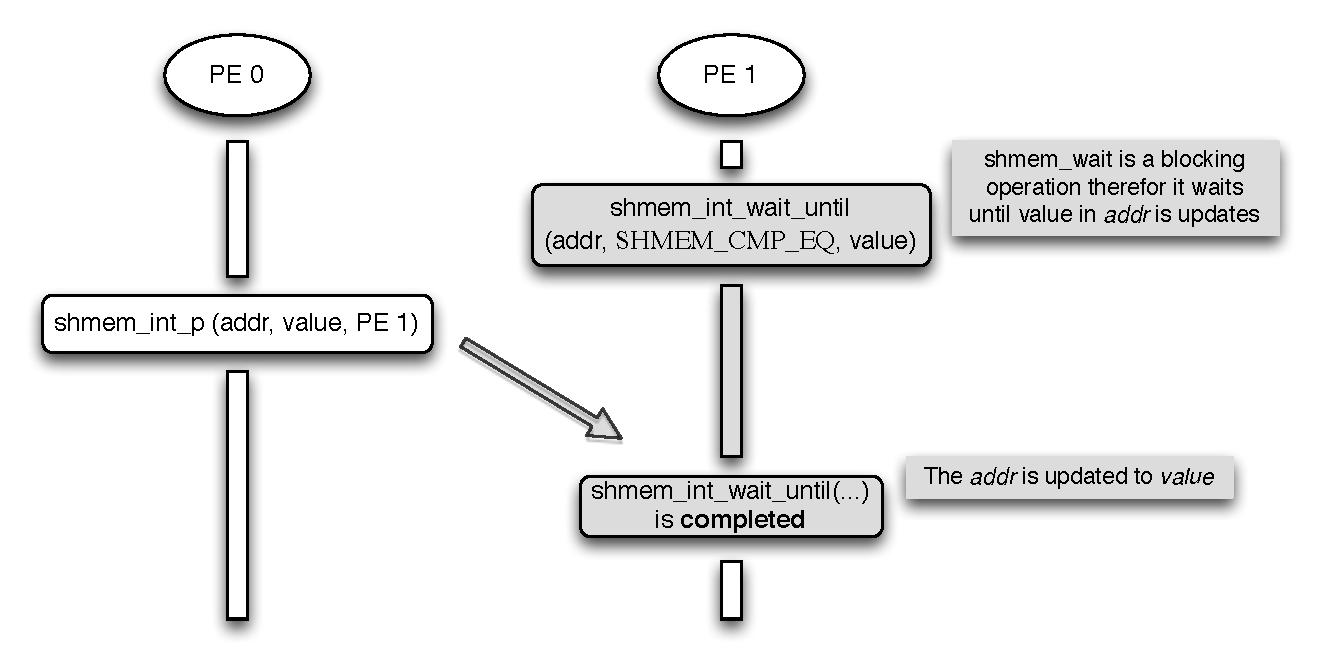
\includegraphics[width=0.7\textwidth]{diagrams/updated/wait}}
\end{tabular}

\begin{tabular}{p{0.2\textwidth} | p{0.7\textwidth}}
{}
&
{ Waits for a symmetric variable to be updated by a remote \ac{PE}. Should be used when computation on the local \ac{PE} cannot proceed without the value that the remote \ac{PE} is to update.} \tabularnewline
\hline 
\end{tabular}

\begin{tabular}{p{0.2\textwidth} | p{0.7\textwidth}}

{Ordering puts issued by a local \ac{PE}} \\
\FUNC{shmem\_fence} 
& 
\raisebox{-\totalheight}{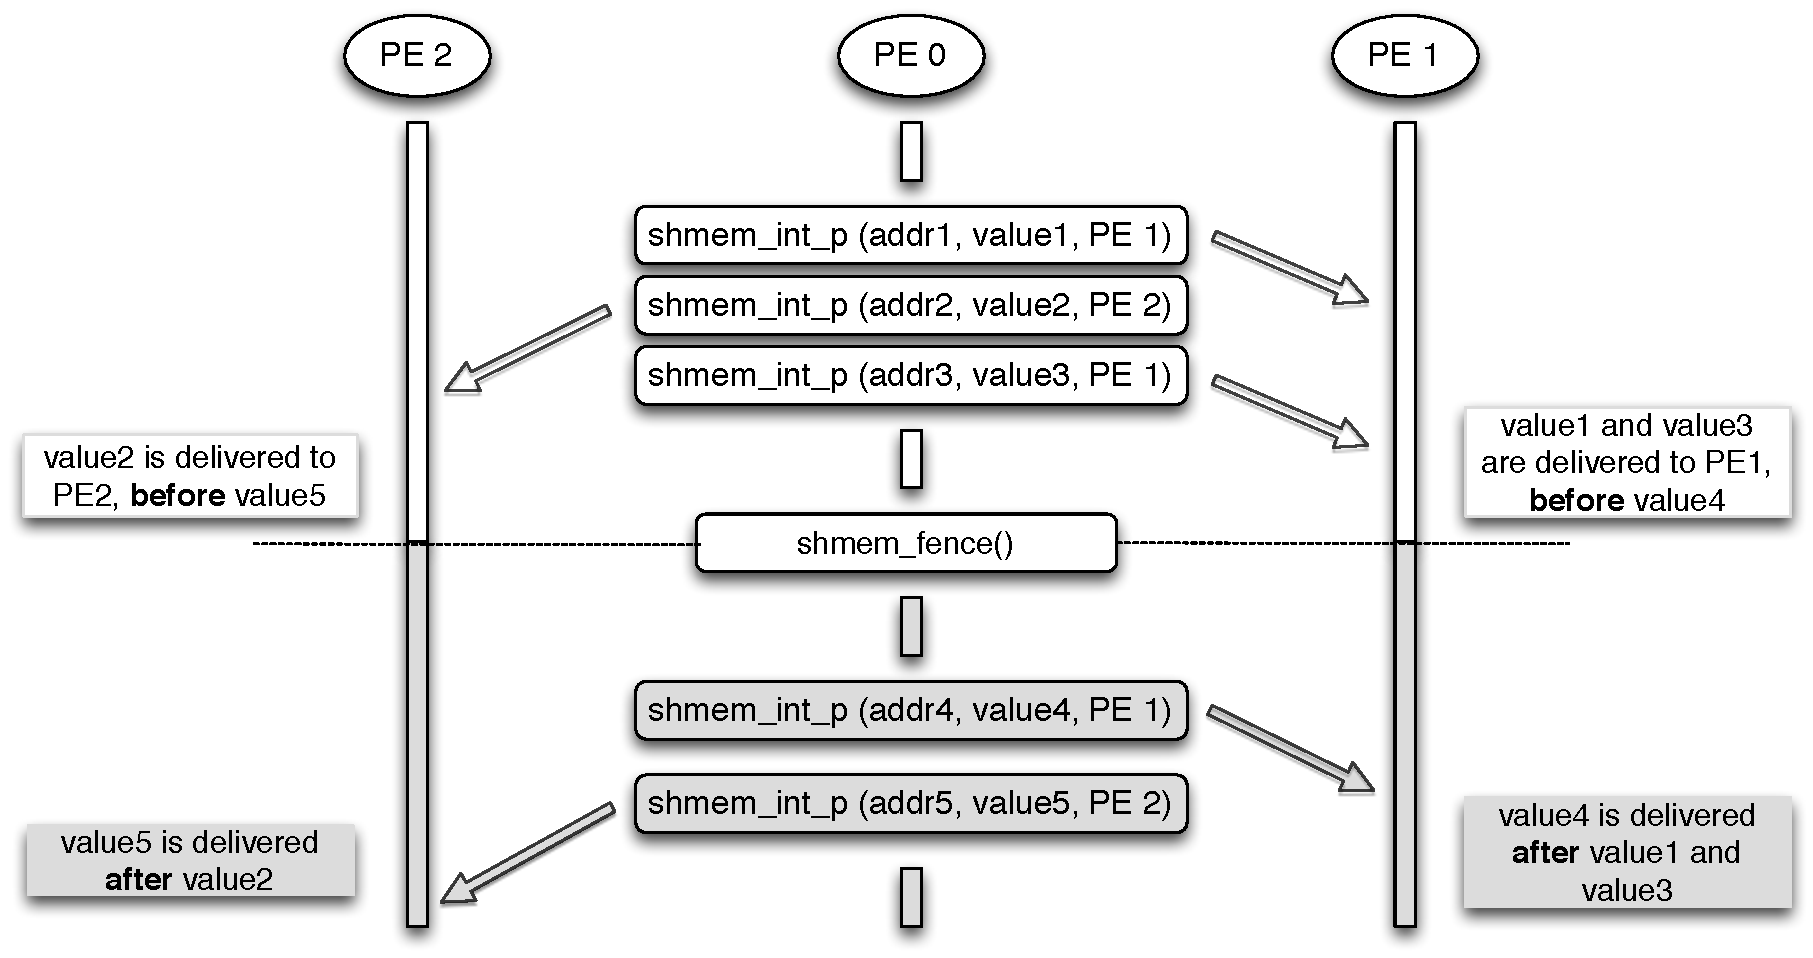
\includegraphics[width=0.7\textwidth]{diagrams/updated/fence}}
\end{tabular}

\begin{tabular}{p{0.2\textwidth} | p{0.7\textwidth}}
{}
&
All \PUT{} routines, \acp{AMO} and store routines on symmetric data issued to same \ac{PE}  are guaranteed to be delivered  before Puts (to the same \ac{PE}) issued after the \FUNC{fence} call. \tabularnewline
%Fence guaranteed order of puts before and after before \Put{}s 
%before the fence operation by the local \ac{PE} are guaranteed to be completed and visible before puts issued after the fence call.
% This operation should be used when all remote writes by a local \ac{PE} to a specific remote \ac{PE} need to be visible %(\rcomment{Swaroop: assuming visible == delivered}) 
%before any new remote write operation to the same \ac{PE}. \tabularnewline
\hline 
\end{tabular}

\begin{tabular}{p{0.2\textwidth} | p{0.7\textwidth}}
\hline 
\textbf{\openshmem  \ac{API}} & \centering \textbf{Working of \openshmem \ac{API}} \tabularnewline
\hline 
\hline
{Ordering puts issued by all \ac{PE} }\\
\FUNC{shmem\_quiet}
& 
\raisebox{-\totalheight}{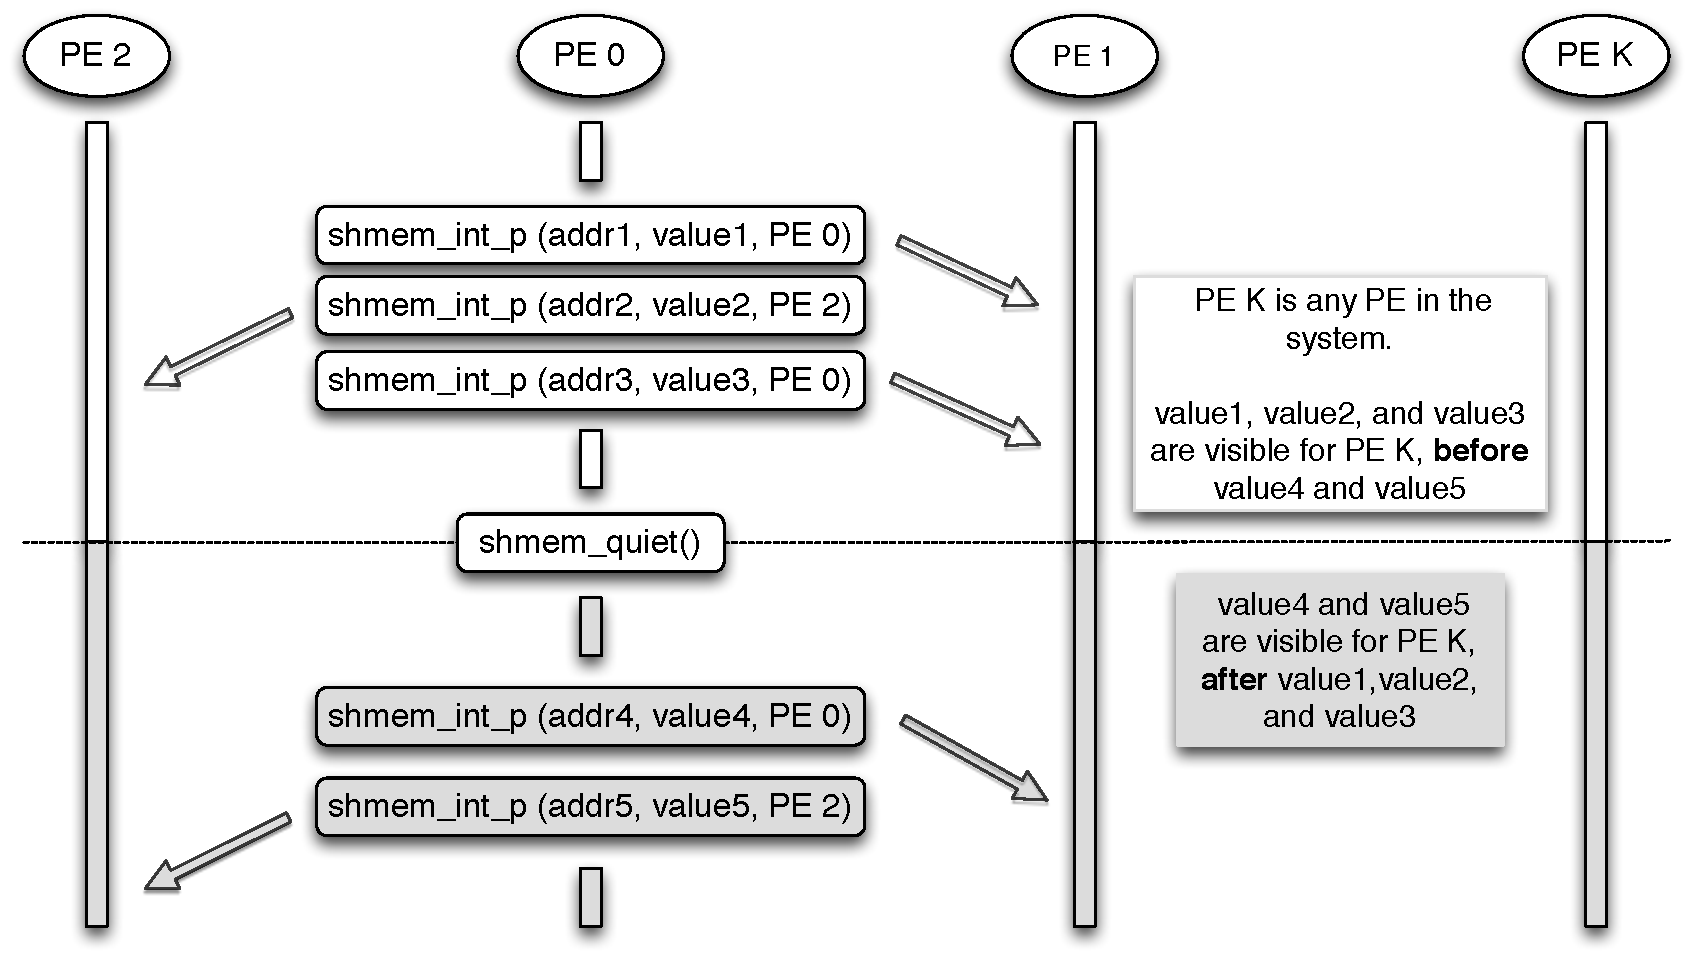
\includegraphics[width=0.7\textwidth]{diagrams/updated/quiet}} 
\end{tabular}

\begin{tabular}{p{0.2\textwidth} | p{0.7\textwidth}}
{}
&
{All \PUT{} routines, \acp{AMO} and store routines on symmetric data issued by a local \ac{PE} to all  remote \ac{PE}s are guaranteed to be completed and visible once quiet returns. This routine should be used when all remote writes issued by a local \ac{PE} need to be visible  to all other \ac{PE}s before the local \ac{PE} proceeds. } \tabularnewline
\hline 
\end{tabular}


\begin{tabular}{p{0.2\textwidth} | p{0.7\textwidth}}
Collective synchronization over an \activeset \\
\FUNC{shmem\_barrier}
&  
\raisebox{-\totalheight}{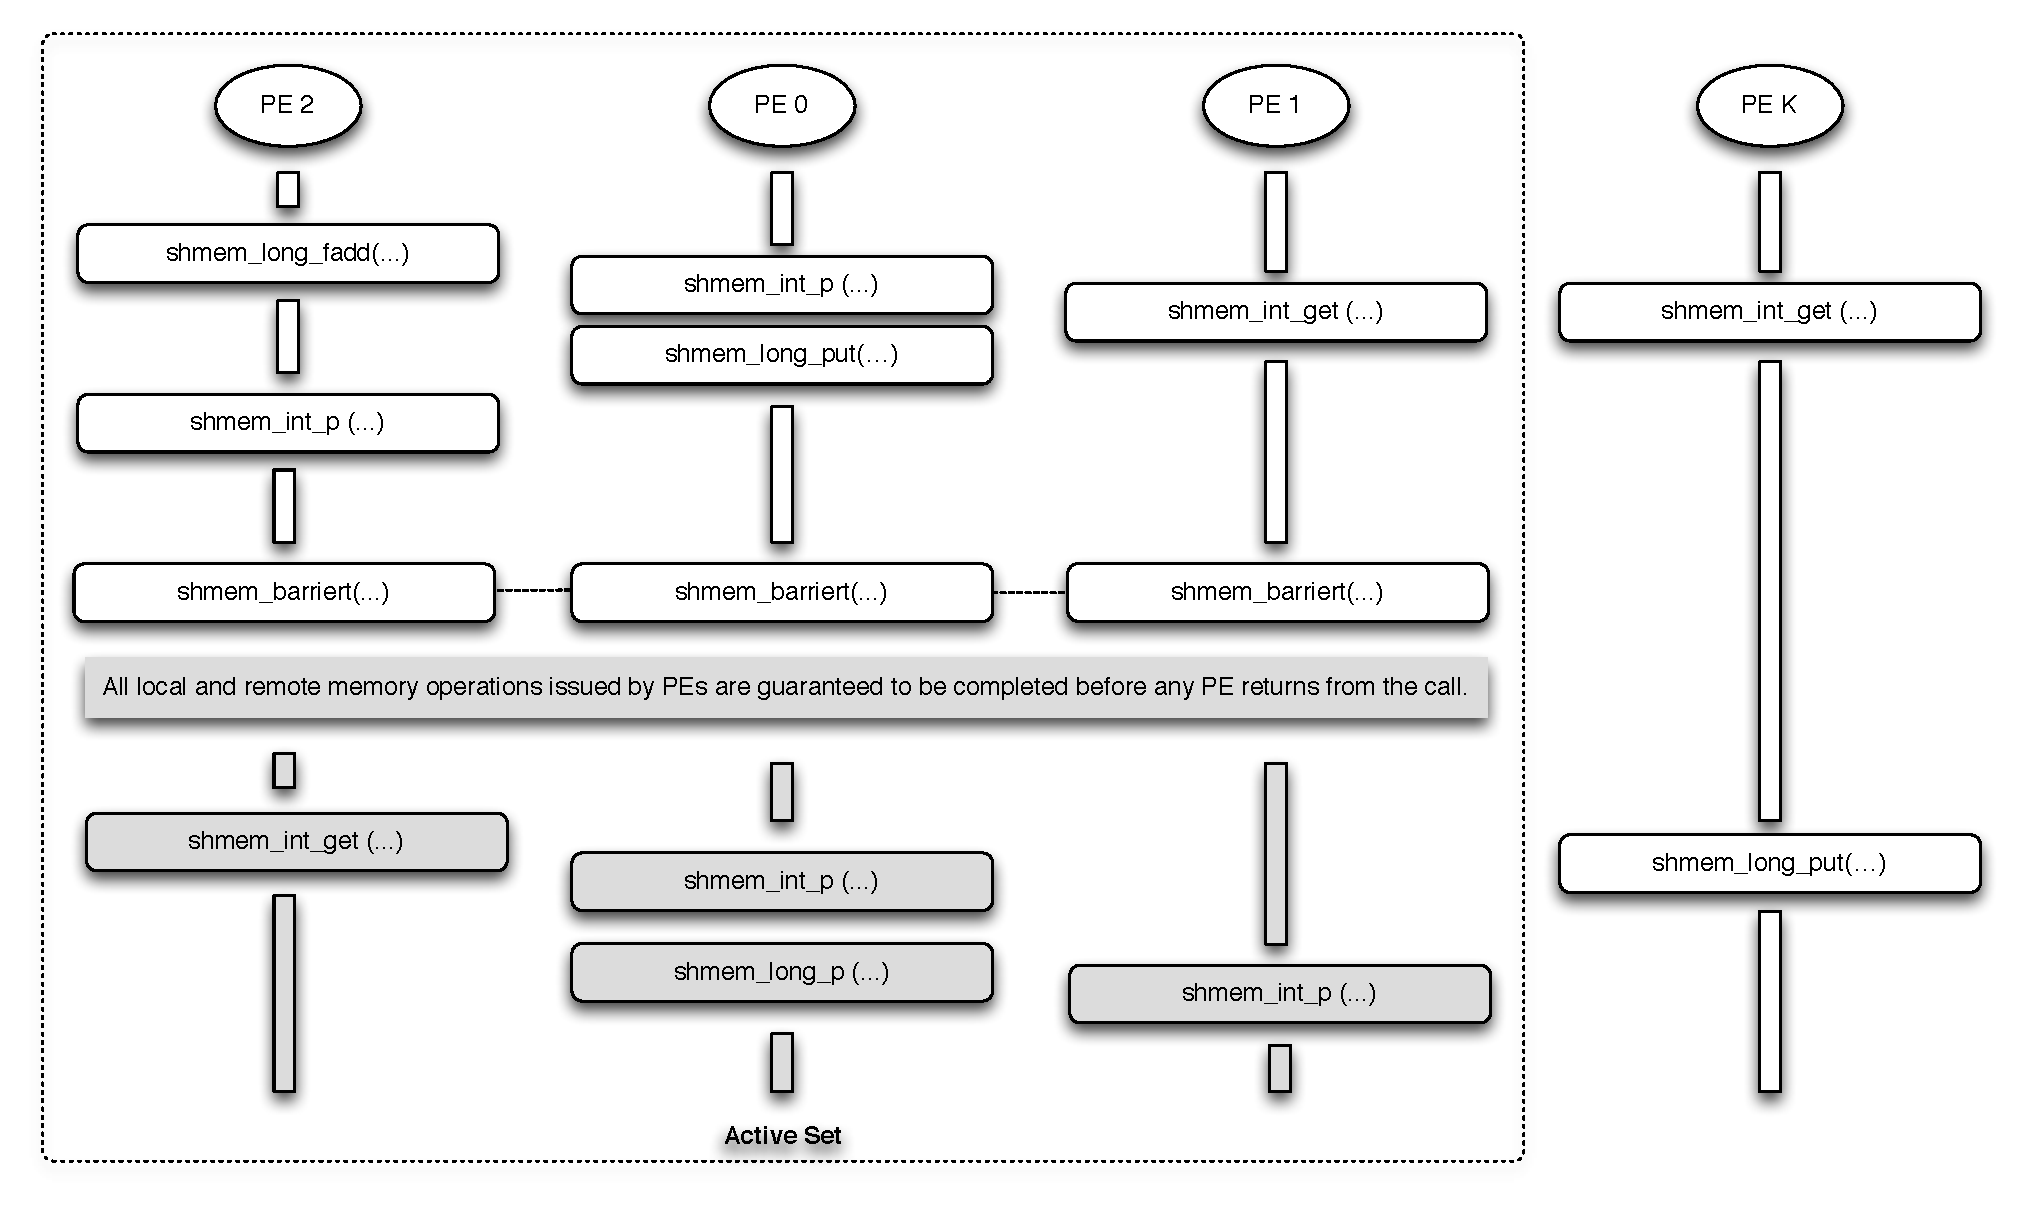
\includegraphics[width=0.7\textwidth]{diagrams/updated/barrier}} 
\end{tabular}

\begin{tabular}{p{0.2\textwidth} | p{0.7\textwidth}}
{}
&
{All local and remote memory operations issued by all \ac{PE}s within the \activeset{} are guaranteed to be completed before any \ac{PE} in the \activeset{} returns from the call. Additionally, no \ac{PE} my return from the barrier until all \ac{PE}s in the \activeset{} have entered the same barrier call. This routine should be used when synchronization as well as completion of all stores and remote memory updates via \openshmem is required over a sub set of the executing \ac{PE}s.} \tabularnewline %Figure (\ref{fig:barrier}).
\hline 
\end{tabular}

\begin{tabular}{p{0.2\textwidth} | p{0.7\textwidth}}
\hline 
\textbf{\openshmem  \ac{API}} & \centering \textbf{Working of \openshmem \ac{API}} \tabularnewline
\hline 
\hline
{Collective synchronization over all \ac{PE}s} \\
 \FUNC{shmem\_barrier\_all}
& 
\raisebox{-\totalheight}{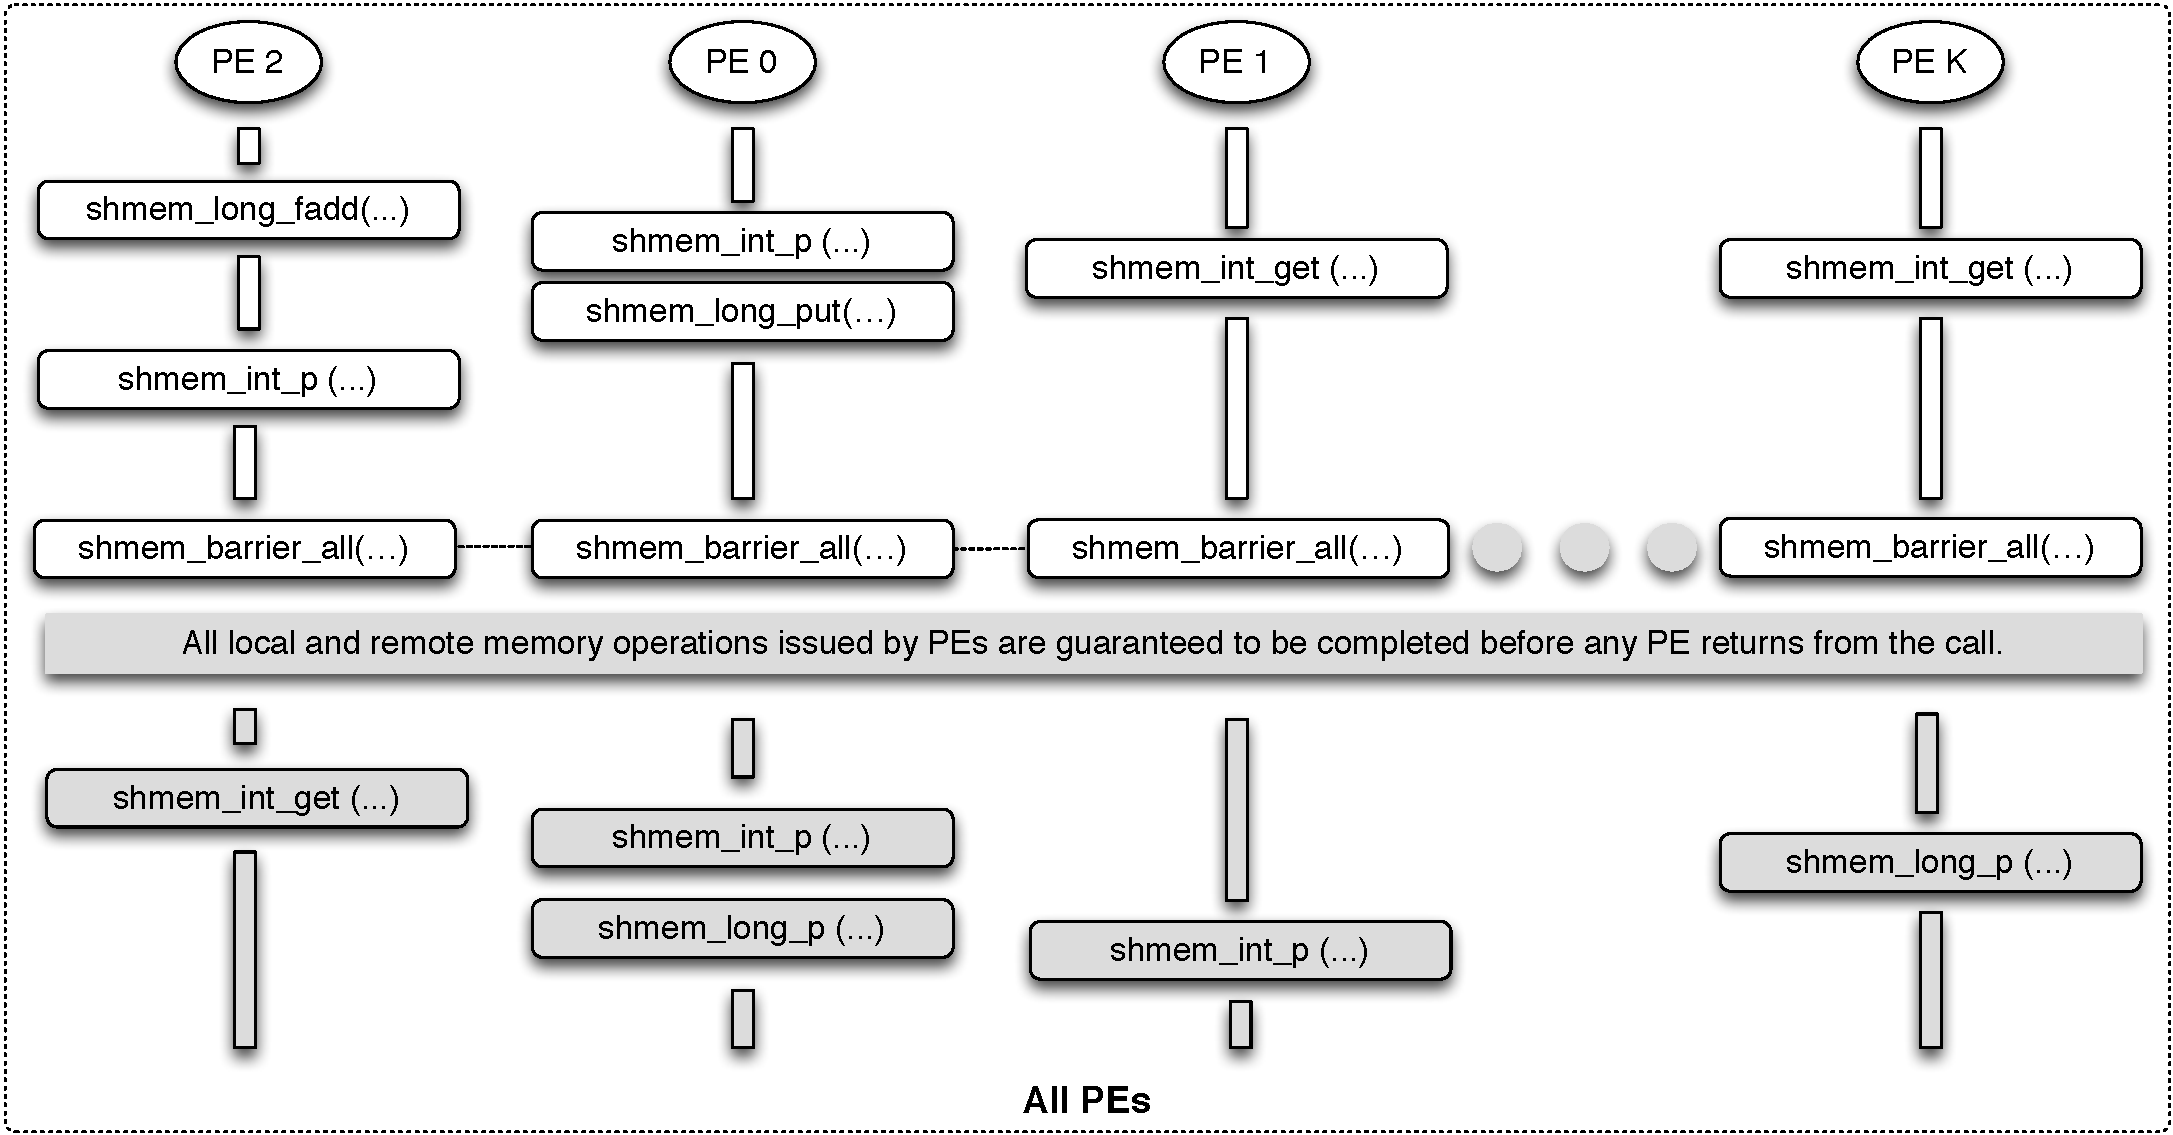
\includegraphics[width=0.7\textwidth]{diagrams/updated/barrierall}}
\end{tabular}

\begin{tabular}{p{0.2\textwidth} | p{0.7\textwidth}}
{}
&
{All local and remote memory operations issued by all \ac{PE}s are guaranteed to be completed before any \ac{PE} returns from the call. Additionally no \ac{PE} shall return from the barrier until all \ac{PE}s have entered the same \FUNC{shmem\_barrier\_all} call. This routine should be used when synchronization as well as completion of all stores and remote memory updates via \openshmem is required over all \ac{PE}s. } \tabularnewline
\hline 
\end{tabular}
\clearpage
%%%%%%%%%%%%%%%%%OLD LAYOUT%%%%%%%%%%%%%%%%
%\begin{tabular}{|p{0.2\textwidth}|p{0.4\textwidth}|p{0.3\textwidth}|}
%\hline 
%\textbf{\openshmem  \ac{API}} & \centering \textbf{Working of \openshmem \ac{API}} & \textbf{Appropriate Situation}\tabularnewline
%\hline 
%\hline 
%{Point-to-point synchronization}\\
%\FUNC{shmem\_wait}, \FUNC{shmem\_wait\_until} 
%&
%\raisebox{-\totalheight}{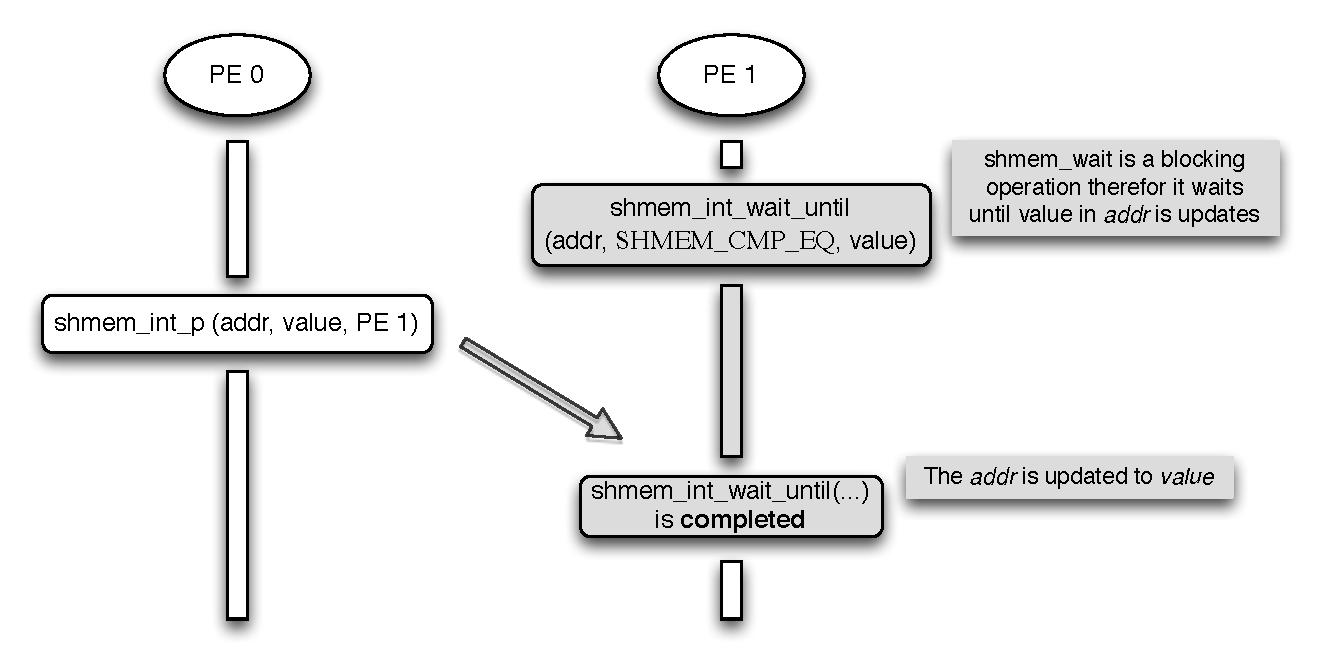
\includegraphics[width=0.39\textwidth]{diagrams/updated/wait}}
%{Waits for a symmetric variable to be updated by a remote \ac{PE}. Should be used when computation at the local \ac{PE} cannot proceed without the value that the remote \ac{PE} is to update.} \tabularnewline
%% Figure (\ref{fig:wait}).}\tabularnewline
%\hline 
%Ordering puts issued by a local \ac{PE} \\
%\FUNC{shmem\_fence} 
%& 
%\raisebox{-\totalheight}{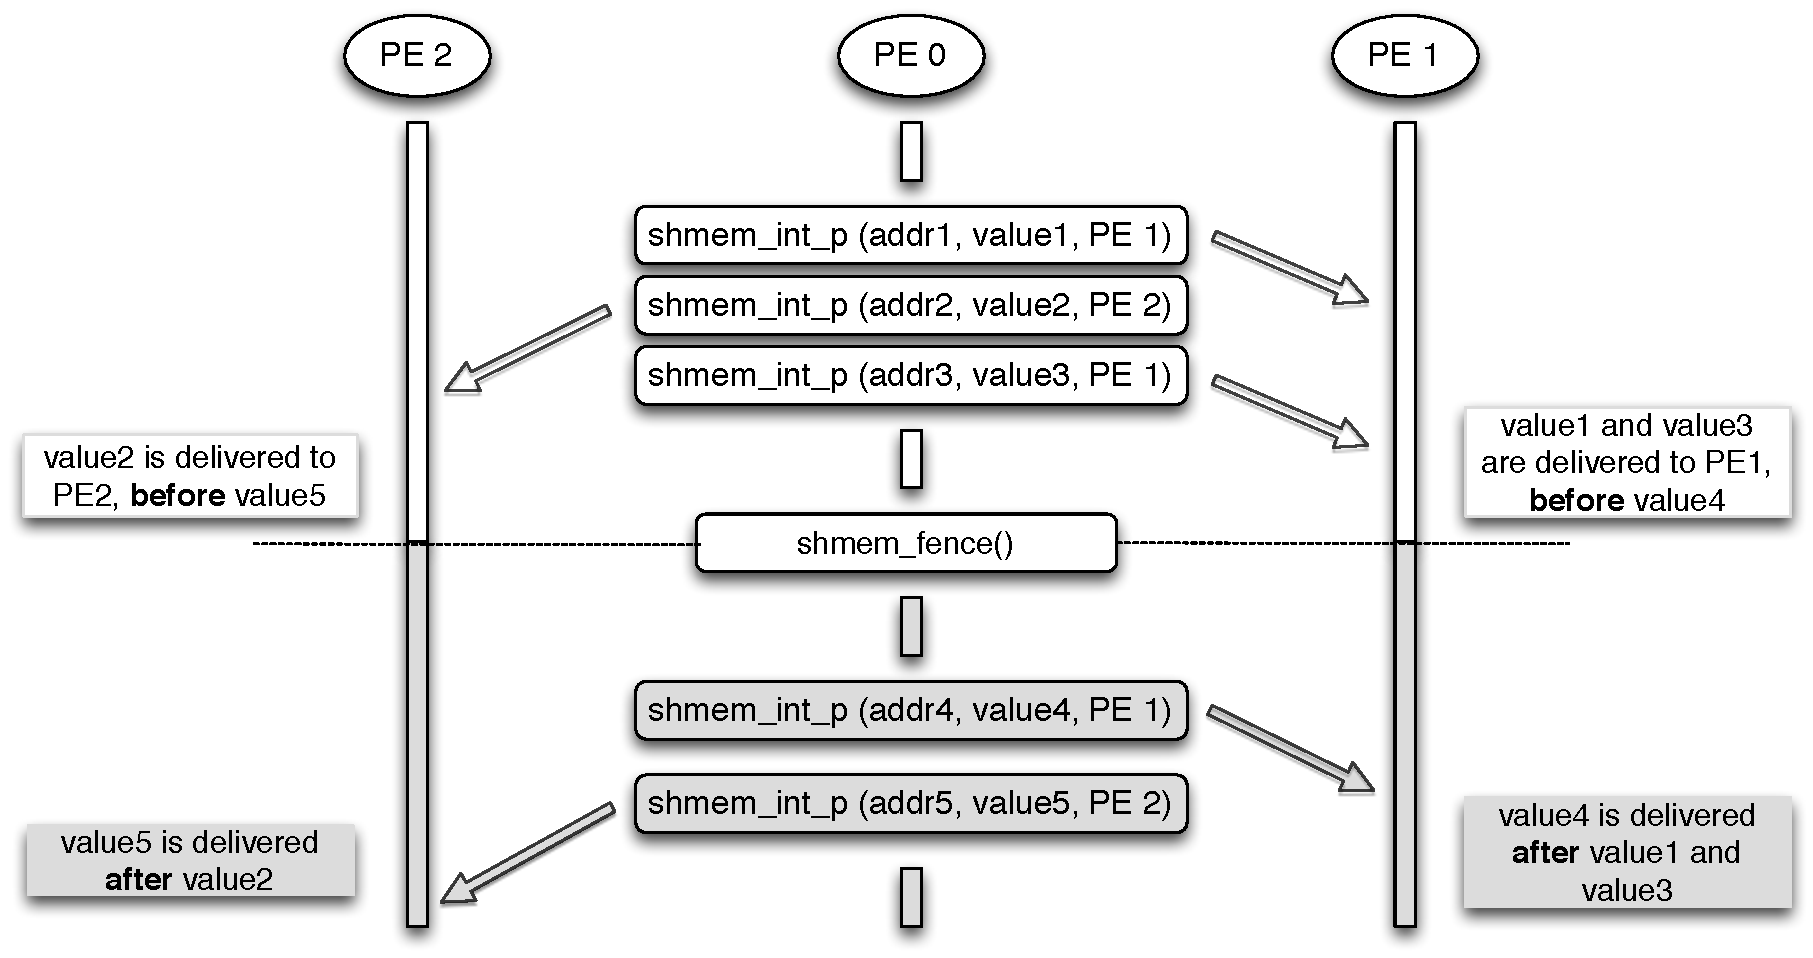
\includegraphics[width=0.39\textwidth]{diagrams/updated/fence}}
%& 
%All puts issued before the fence operation by the local \ac{PE} are guaranteed to be delivered before puts issued after the fence call to the same remote \ac{PE}. This operation should be used when all remote writes by a local \ac{PE} to a remote \ac{PE} need to be visible %(\rcomment{Swaroop: assuming visible == delivered}) 
%before any new remote write operation to the same \ac{PE}. \tabularnewline
%%Figure (\ref{fig:fence}).\tabularnewline
%\hline 
%Ordering puts issued by all \ac{PE} \\
%\FUNC{shmem\_quiet}
%& 
%\raisebox{-\totalheight}{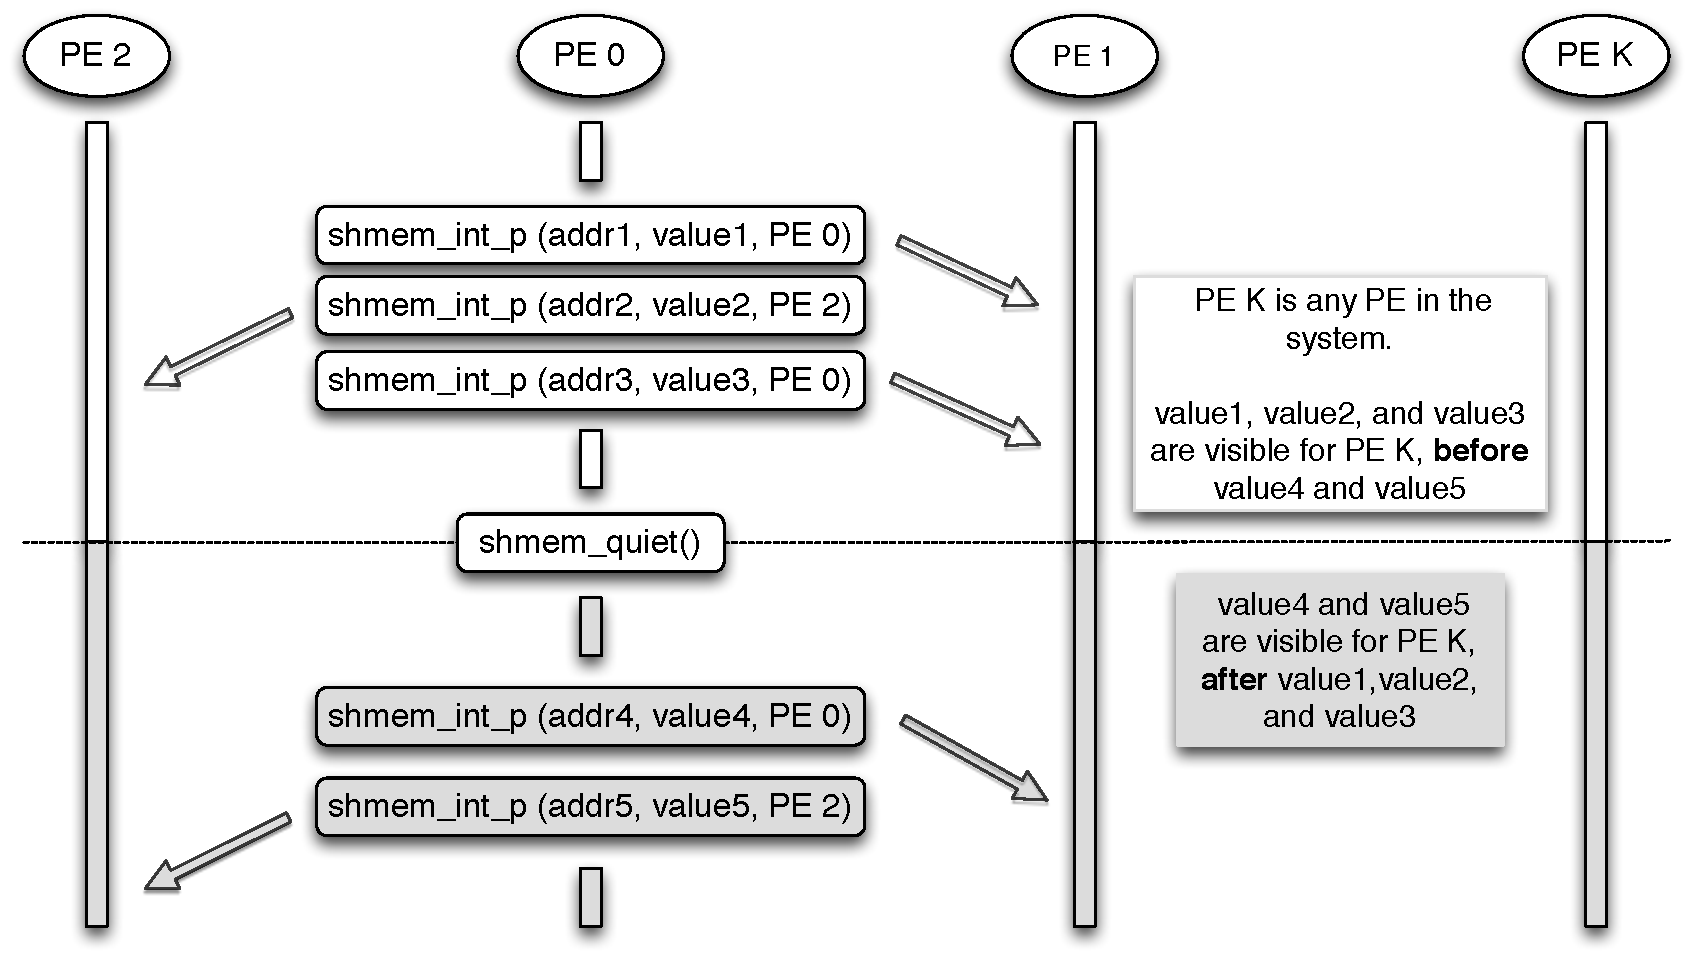
\includegraphics[width=0.39\textwidth]{diagrams/updated/quiet}} 
%& 
%{All puts issued by all \ac{PE}s are guaranteed to be delivered before the next local update or remote memory update via \openshmem (\rcomment{May change after SGI's input.}). This operation should be used when all remote writes by all \ac{PE}s need to be visible  to all other \ac{PE}s before any new local or remote memory update via \openshmem library operation. } \tabularnewline
%%Figure (\ref{fig:quiet}).} \tabularnewline
%\hline 
%\end{tabular}
%\clearpage
%\begin{tabular}{|p{0.2\textwidth}|p{0.4\textwidth}|p{0.3\textwidth}|}
%\hline 
%Collective synchronization over an \activeset \\
%\FUNC{shmem\_barrier}
%&  
%\raisebox{-\totalheight}{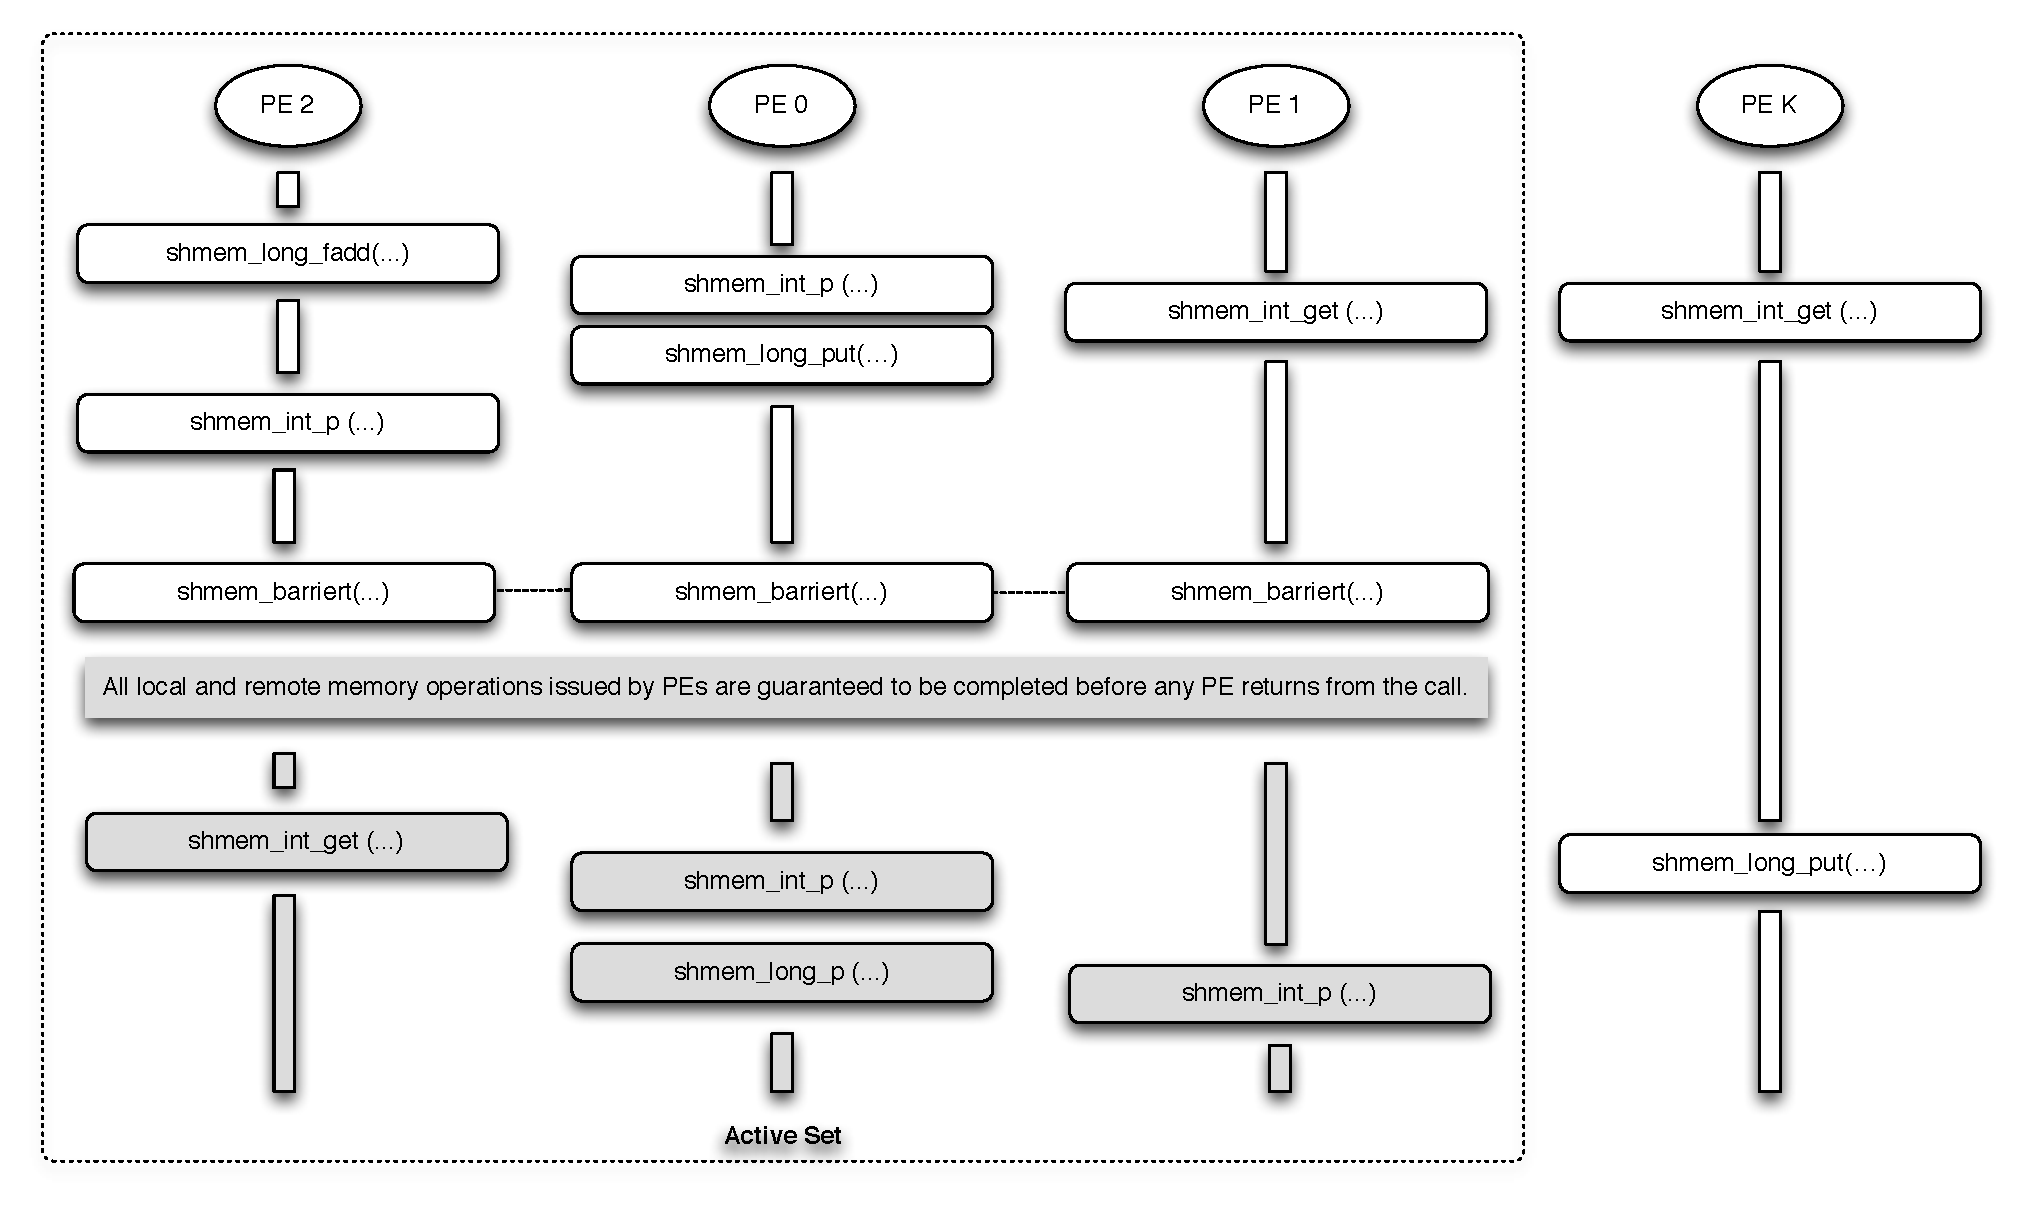
\includegraphics[width=0.39\textwidth]{diagrams/updated/barrier}} 
%& 
%{All local and remote memory operations issued by all \ac{PE}s within the \activeset{} are guaranteed to be completed before any \ac{PE} in the \activeset{} returns from the call. Additionally no \ac{PE} my return from the barrier till all \ac{PE}s in the \activeset{} have called the same barrier call. This operation should be used when synchronization as well as completion of local stores and remote memory updates via \openshmem is required over a sub-set of the executing \ac{PE}s.} \tabularnewline %Figure (\ref{fig:barrier}).
%\hline 
%Collective synchronization over all \ac{PE}s \\
% \FUNC{shmem\_barrier\_all}
%& 
%\raisebox{-\totalheight}{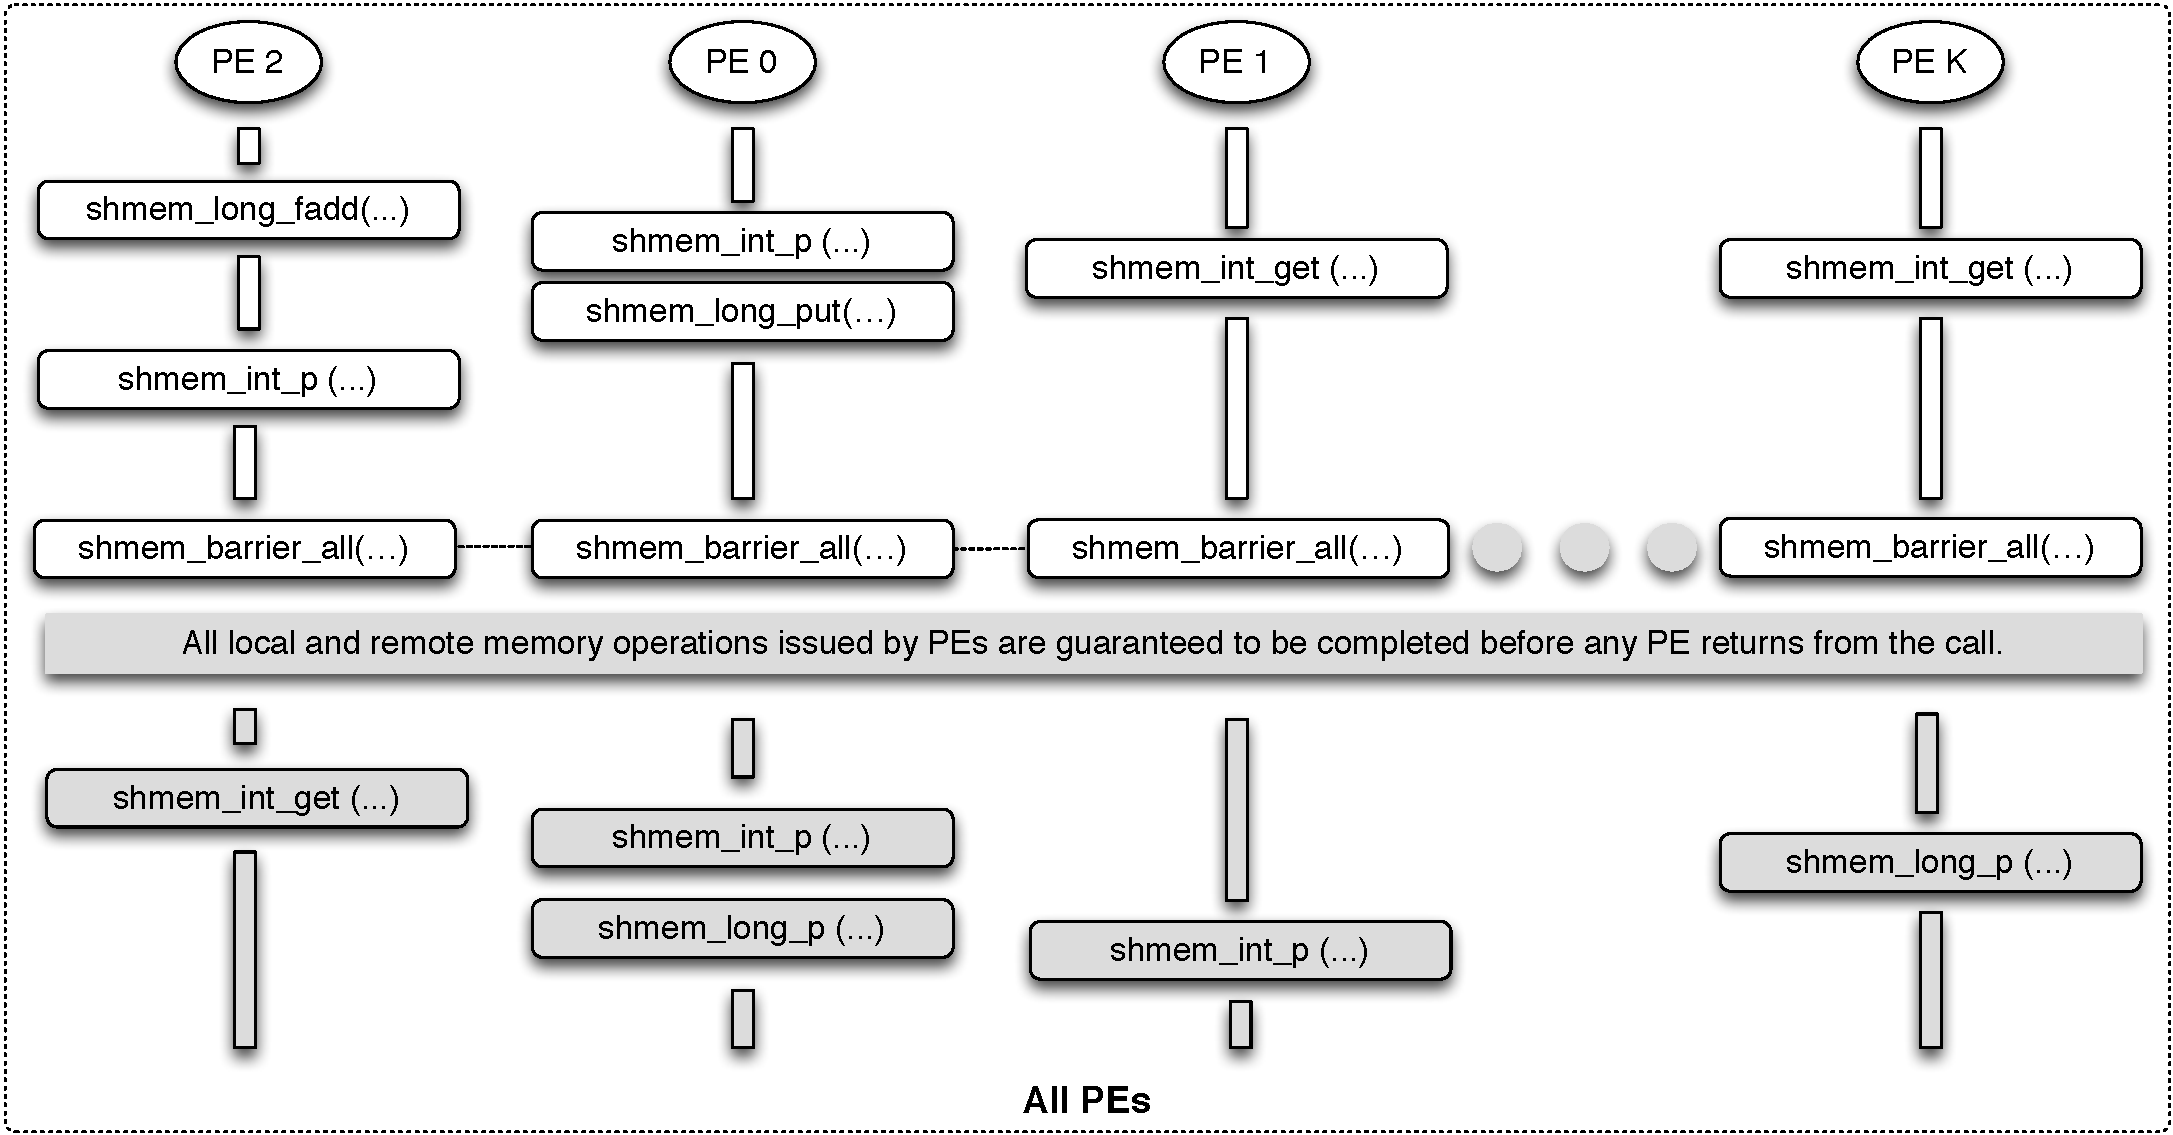
\includegraphics[width=0.39\textwidth]{diagrams/updated/barrierall}}
%& 
%{All local and remote memory operations issued by all \ac{PE}s are guaranteed to be completed before any \ac{PE} returns from the call. Additionally no \ac{PE} my return from the barrier until all \ac{PE}s have called the same barrier call. This operation should be used when synchronization as well as completion of local stores and remote memory updates via \openshmem is required over all \ac{PE}s. } \tabularnewline%Figure (\ref{fig:barrierall}).
%
%\hline 
%\end{tabular}


%\begin{figure}
%%        \centering
%        \begin{subfigure}{0.5\textwidth}
%                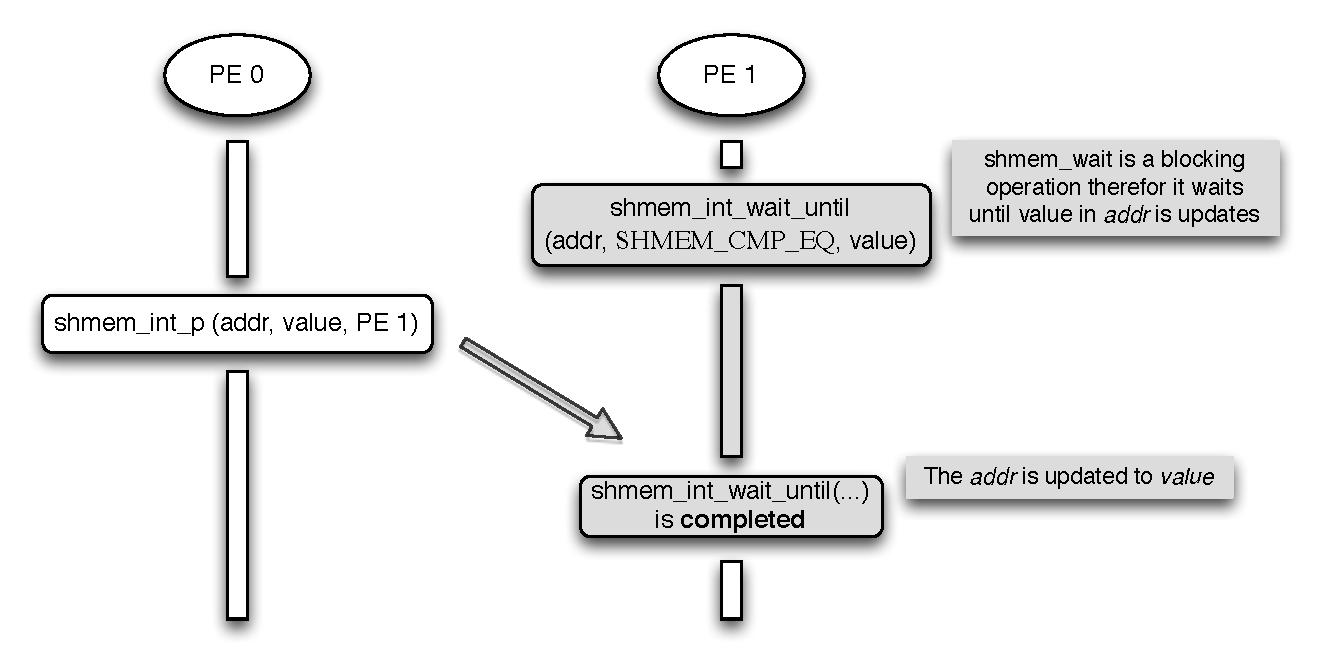
\includegraphics[width=\textwidth]{diagrams/updated/wait}
%                \caption{\FUNC{shmem\_wait}}
%                \label{fig:wait}
%        \end{subfigure}
%        \begin{subfigure}{0.49\textwidth}
%                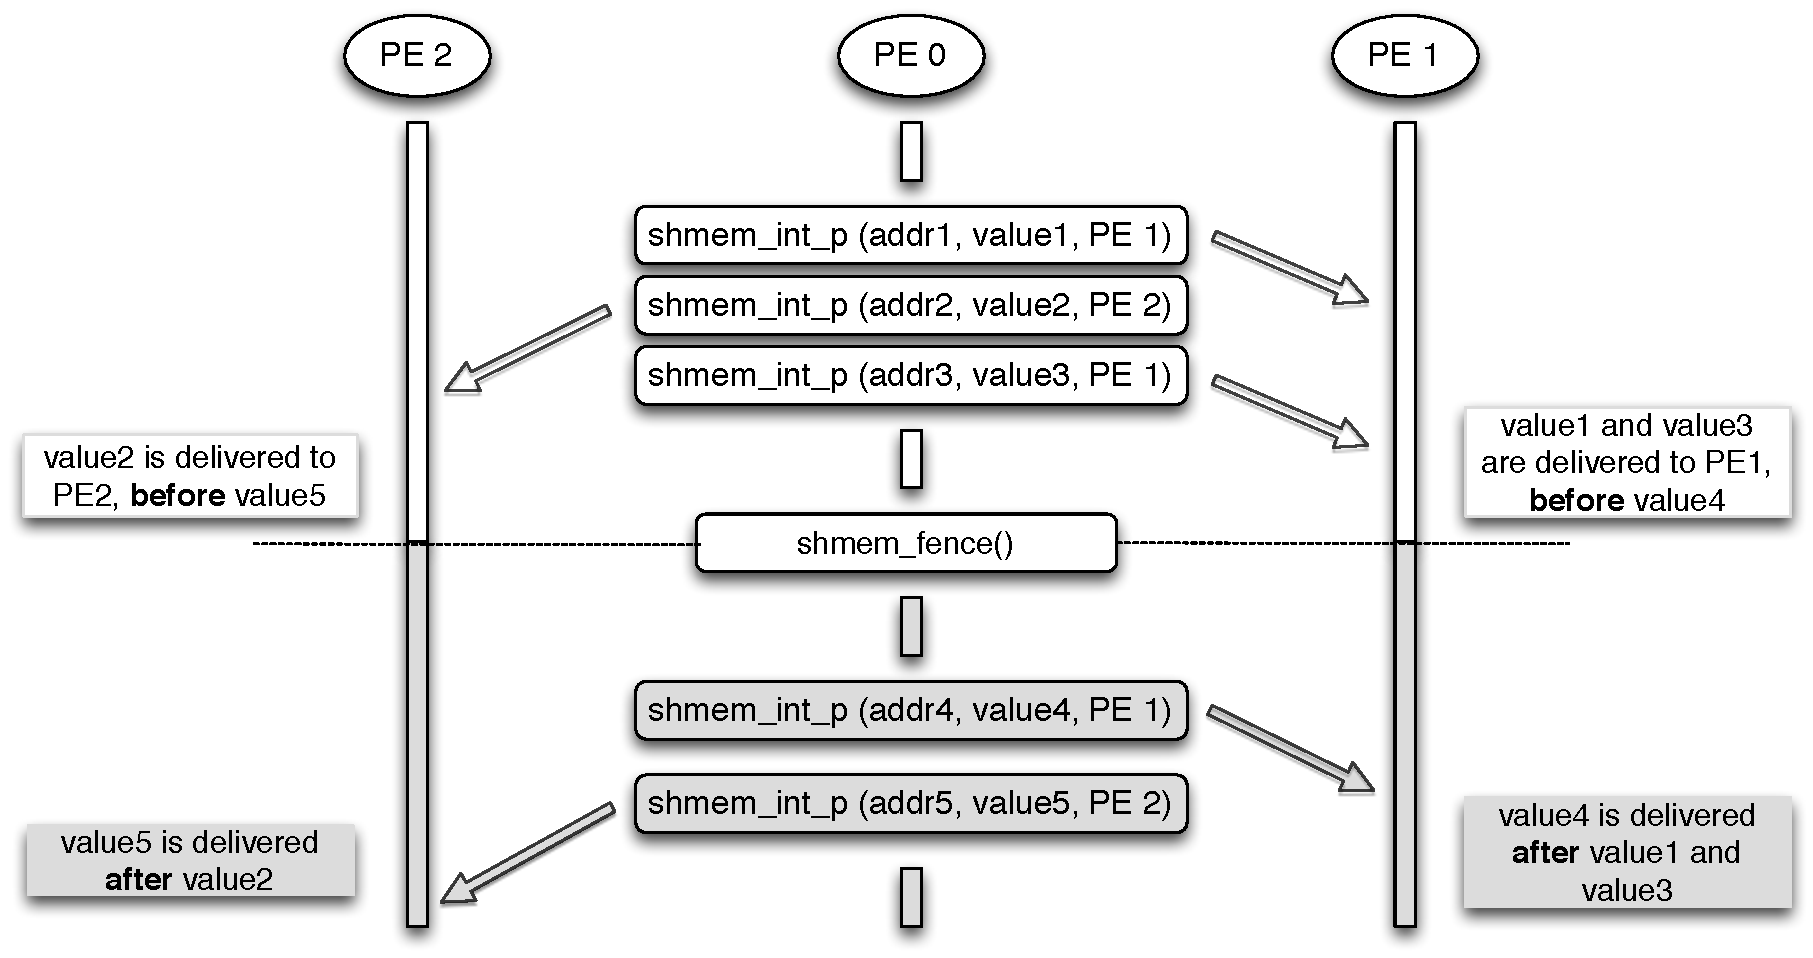
\includegraphics[width=\textwidth]{diagrams/updated/fence}
%                \caption{\FUNC{shmem\_fence}}
%                \label{fig:fence}
%        \end{subfigure}
%        \begin{subfigure}{0.48\textwidth}
%                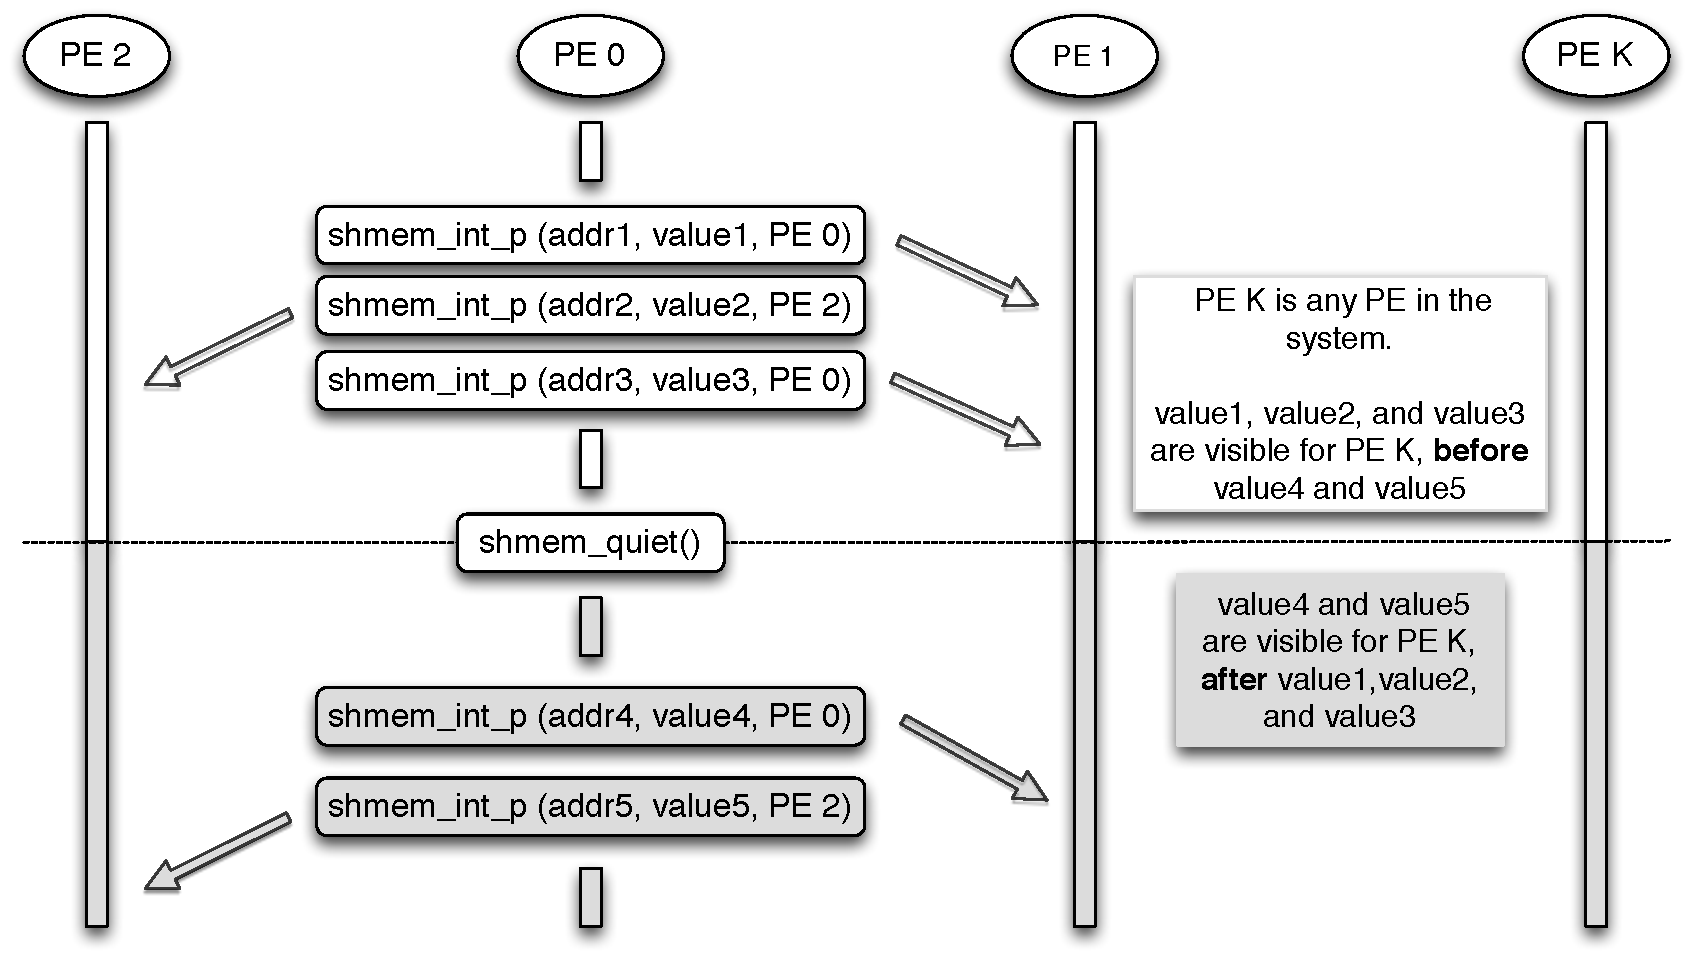
\includegraphics[width=\textwidth]{diagrams/updated/quiet}
%                \caption{\FUNC{shmem\_quiet}}
%                \label{fig:quiet}
%        \end{subfigure}
%	    \begin{subfigure}{0.48\textwidth}
%		        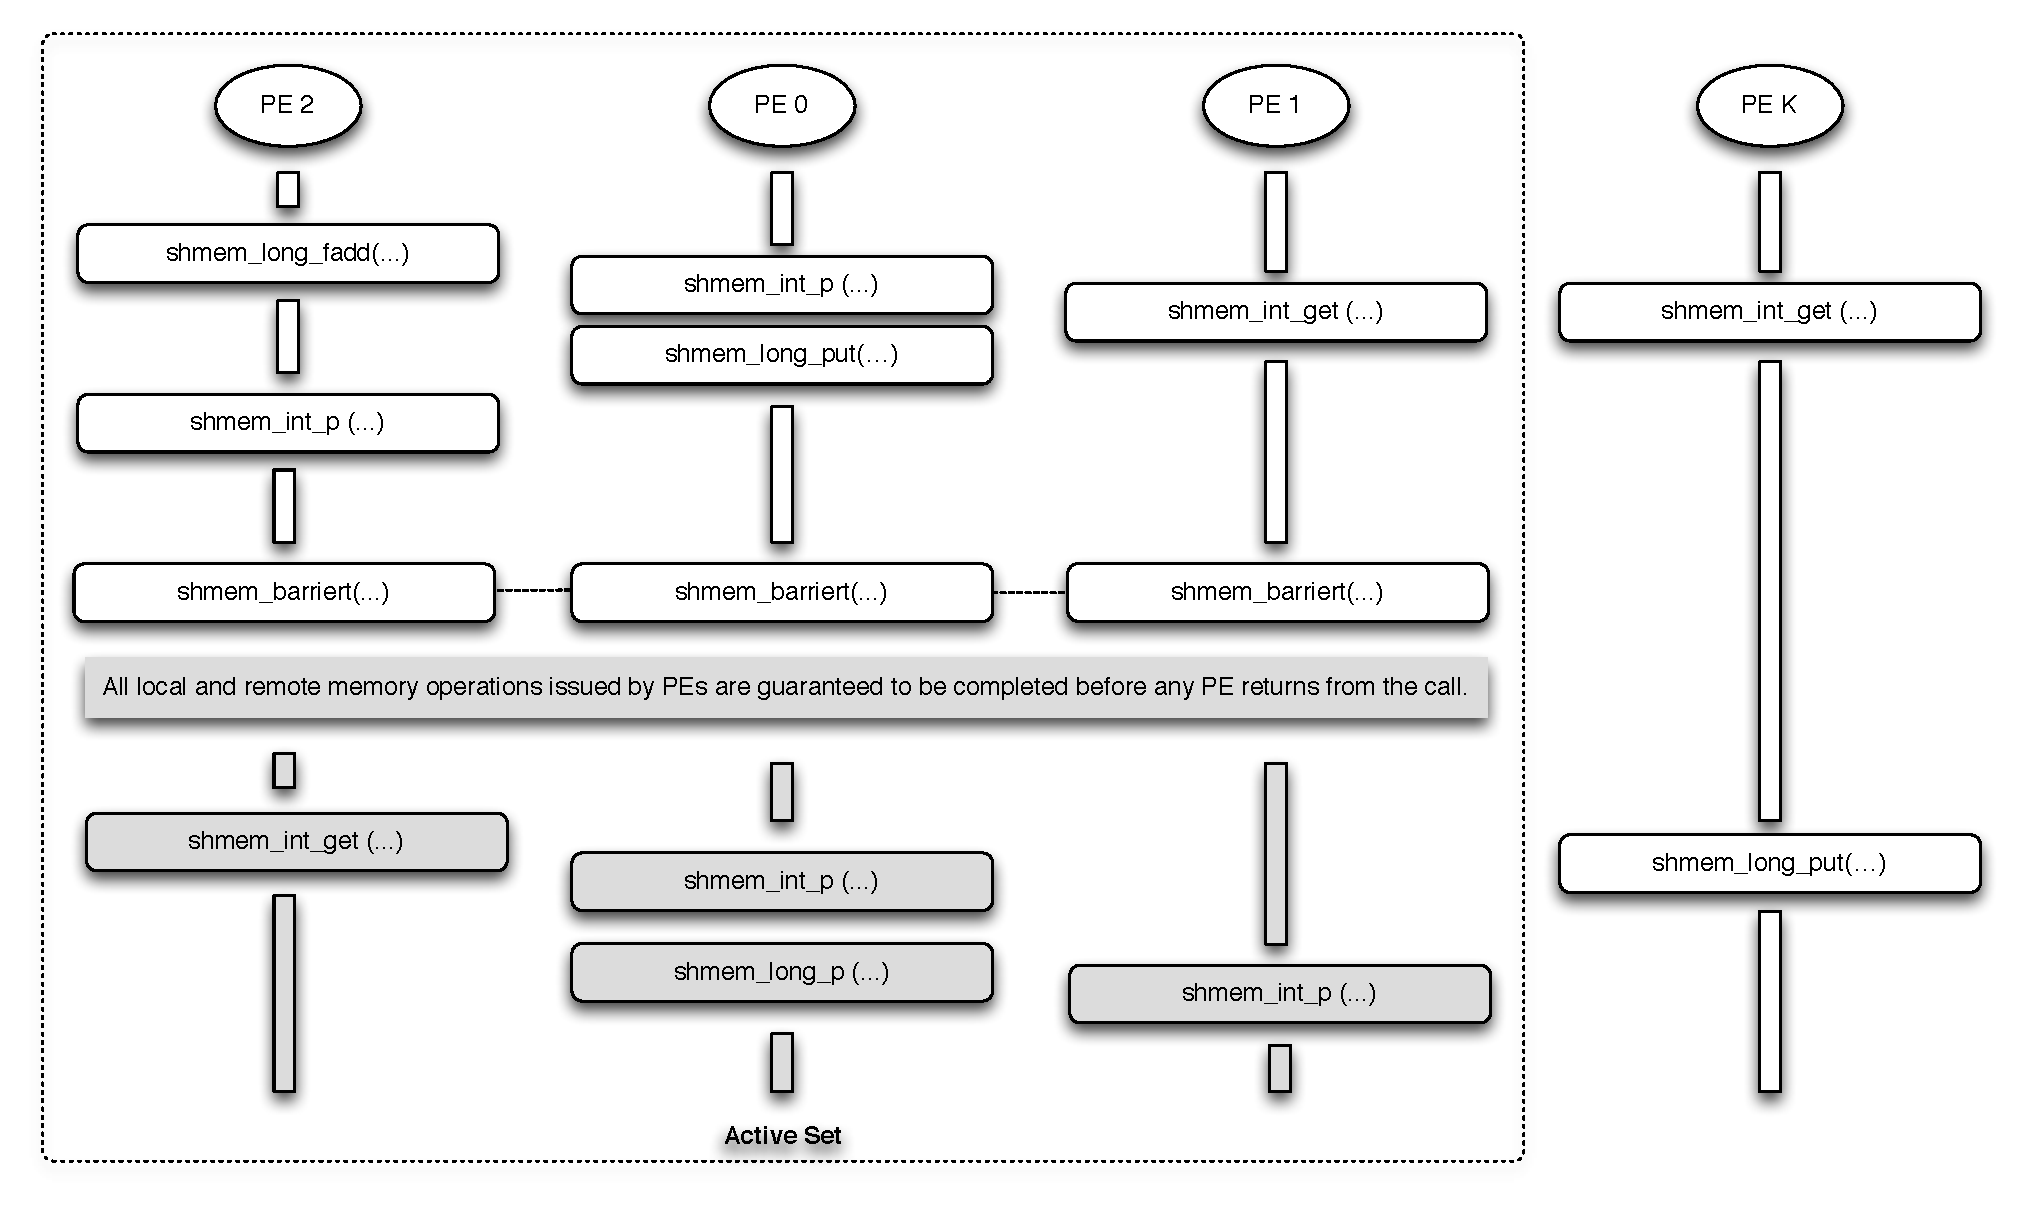
\includegraphics[width=\textwidth]{diagrams/updated/barrier}
%		        \caption{\FUNC{shmem\_barrier}}
%		\label{fig:barrier}
%	    \end{subfigure}
%        \centering
%	    \begin{subfigure}{0.48\textwidth}
%		        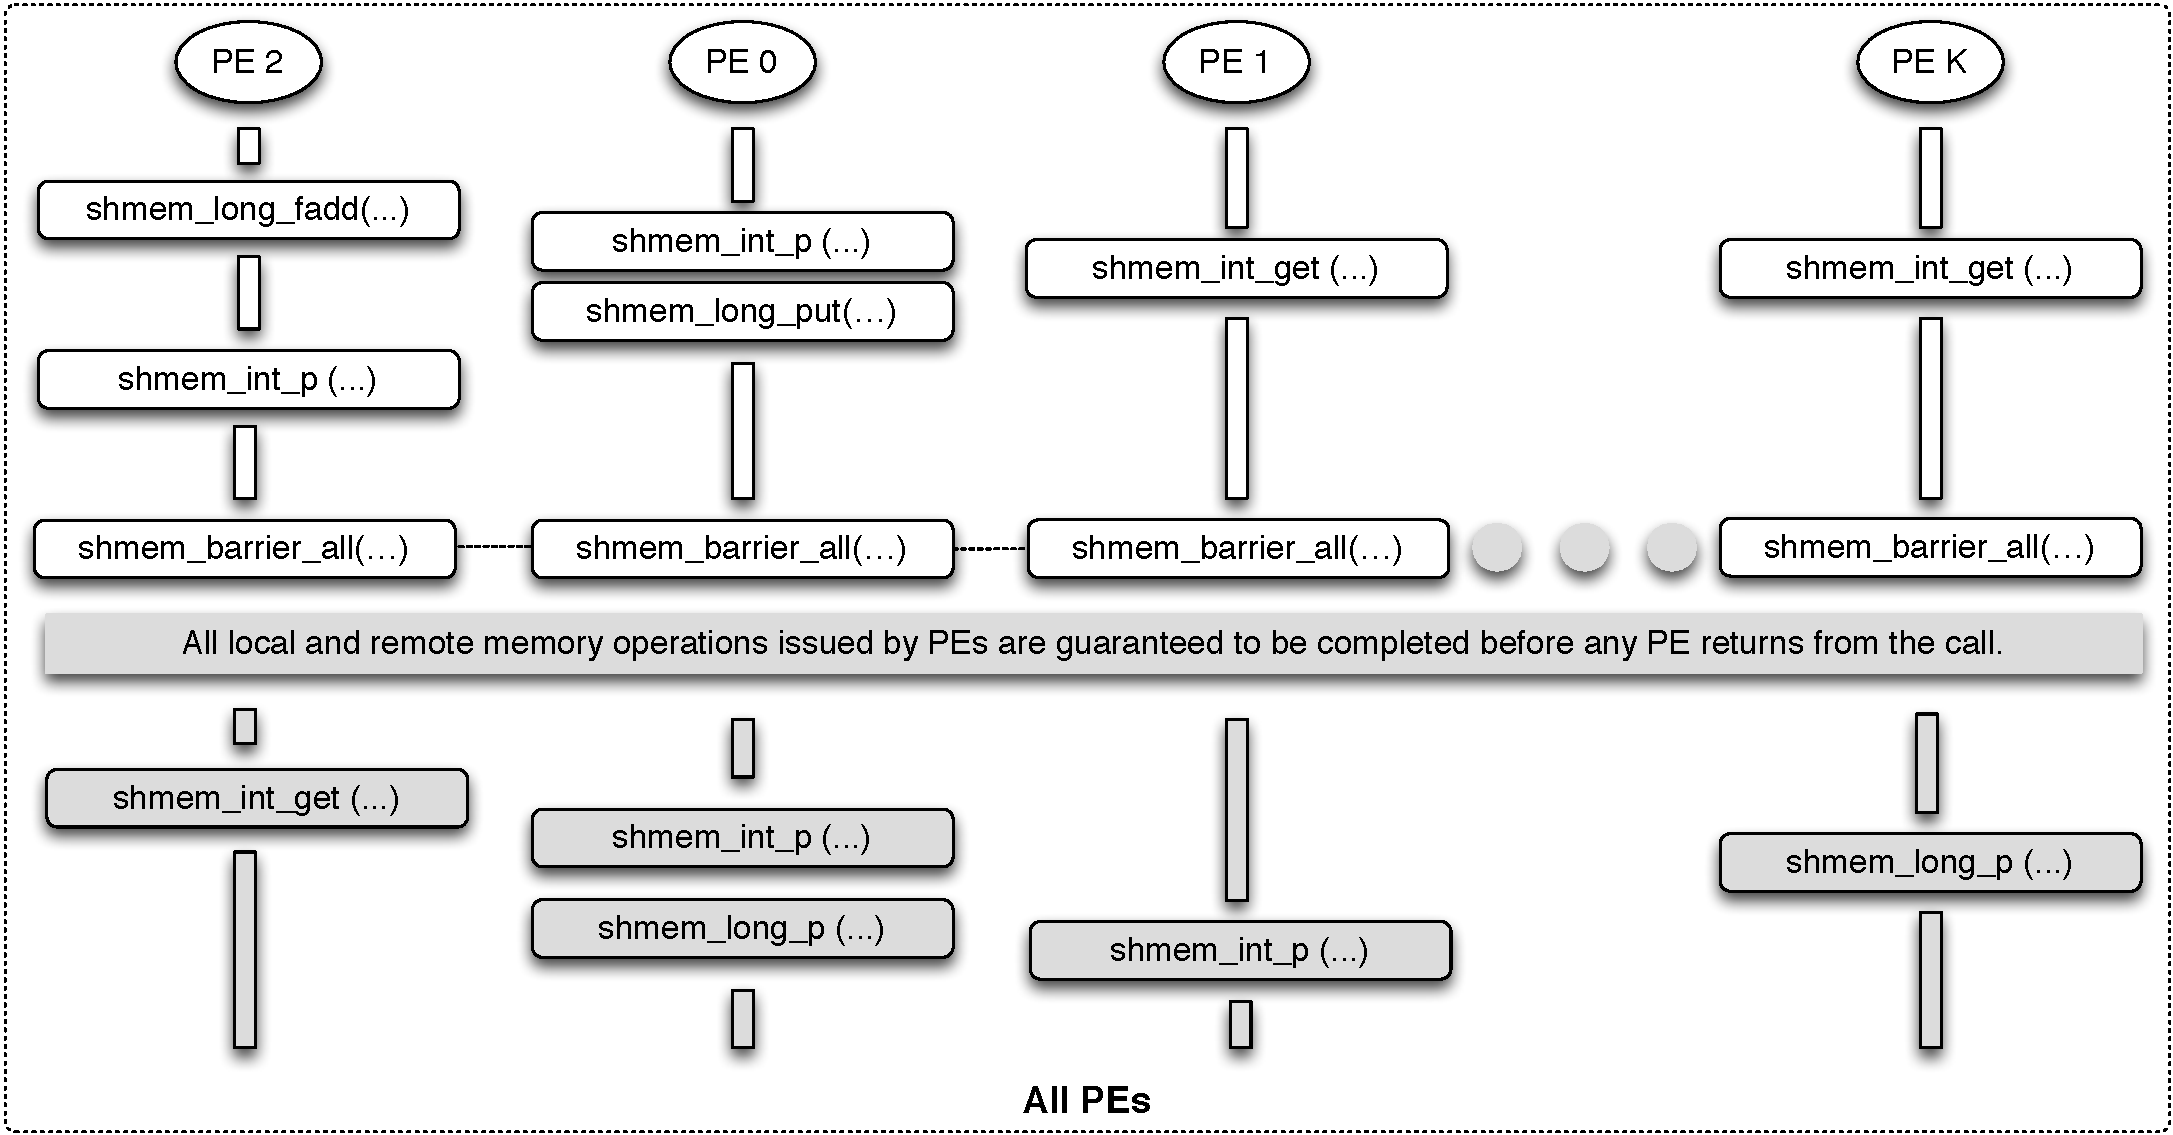
\includegraphics[width=\textwidth]{diagrams/updated/barrierall}
%		        \caption{\FUNC{shmem\_barrierall}}
%		\label{fig:barrierall}
%	    \end{subfigure}
%        \caption{\openshmem{} synchronization operations}\label{fig:animals}
%\end{figure}
 %SP:Moving to remote memory operations section as per discussion on 1/21/14

\clearpage

\startchap
\section{OpenSHMEM Library API}
\subsection{Library Setup and Query Operations}%SP: Merging two operations 
\bAPI{START\_PES}{Called  at the beginning of an \openshmem program to initialize the execution environment.}
\synC   %Synopisis for C API 
void start_pes(int npes);
%*\synCE    %DO NOT DELETE. THIS LINE IS NOT A COMMENT

\synF   %Synopsis for FORTRAN API
CALL START_PES(npes)
 %*\synFE   %DO NOT DELETE. THIS LINE IS NOT A COMMENT  

% Arguments table. If no arguments you can use \argRow{NONE}{}{} 
\desB{  
       \argRow{npes}{	 Unused}{ Should be set to 0.}
}
 %API description
 {   The start\_pes routine should be the first statement in a OpenSHMEM parallel
       program.
 }
 %API Description Table. 
{
    {} 
 %Return Values     
\desR{ None. }

\notesB{ If  the	start\_pes  call	 is  not  the  first  statement in a program,  unexpected results may occur.}

}%end of DesB
% Notes. If there are no notes, this field can be left empty.


%Example
\exampleB{
%For each example, you can enter it as an item.
                  \exampleITEMF
                  { This is a simple program that calls shmem\_integer\_put():}
                 {./EXAMPLES/shmem_startpes_example.f90}
 {} 
}  	
\eAPI 
 %Swaroop
\bAPI{SHMEM\_MY\_PE}{Returns the number of the calling \ac{PE}.}

%Synopsis C
\synC
int shmem_my_pe(void);
int _my_pe (void);
%*\synCE

%Synopsis F
\synF 
INTEGER SHMEM_MY_PE, ME
MYPE = SHMEM_MY_PE()
ME = MY_PE ()
%*\synFE

%DESCRIPTION

%Arguments
\desB{
	\argRow{NONE}{}{}
}
%API Description
{
	This function returns the processing element (\ac{PE}) number of the calling
  \ac{PE}.   It accepts no arguments.	The result is an integer between \CONST{0} and
  \VAR{npes} - \CONST{1}, where \VAR{npes} is the total number of \ac{PE}s executing  the  current
  program.
}
%API Description Table.
{
%	\desTB{ }
%	{
%				\cRow{}{}
%	}

	%Return Value       
  \desR{Integer - Between \CONST{0} and \VAR{npes} - \CONST{1}}

	%NOTES
	\notesB{
		For \openshmem Specification 1.1 the use of \FUNC{\_my\_pe} has been deprecated. Although \openshmem libraries are required to support the call, application developers are encouraged to use \FUNC{shmem\_my\_pe} instead.
     }
}
%EXAMPLES
\exampleB{
		\exampleITEM
       {The following \FUNC{shmem\_my\_pe} example is for C/C++ programs:}
			 {./EXAMPLES/shmem_mype_example.c}
			 {}
}
\eAPI
 %Tommy
\bAPI{SHMEM\_N\_PES}{Returns the number of \ac{PE}s running in a program.}
%Synopsis C
\synC
int shmem_n_pes(void);
int _num_pes (void); %*\synCE

%Synopsis F
\synF
INTEGER SHMEM_N_PES, N_PES
N_PES = SHMEM_N_PES()
N_PES = NUM_PES() %*\synFE

%DESCRIPTION

%Arguments
\desB{
	\argRow{None}{}{}
}
%API Description
{
	The function returns the number of \ac{PE}s running the program.
}
%API Description Table.
{
%		\desTB{}
%		{
%				\cRow{}{}
%		}
		%Return Value
		\desR{Integer -  Number of \ac{PE}s running the \openshmem program.}
		%NOTES      
	\notesB{As of \openshmem Specification 1.2 the use of \FUNC{\_num\_pes} has been deprecated. Although \openshmem libraries are required to support the call, program developers are encouraged to use \FUNC{shmem\_n\_pes} instead.
}
		}
		%EXAMPLES
\exampleB{
	\exampleITEM
	{The following \FUNC{\_num\_pes} example is for \CorCpp{} programs:}
	{./EXAMPLES/shmem_npes_example.c}
	{}
}
\eAPI

%Tommy
\bAPI{SHMEM\_PE\_ACCESSIBLE}{Determines whether a \ac{PE} is accessible via \openshmem's data transfer operations.}
\synC     
int shmem_pe_accessible(int pe); %*\synCE    %DO NOT DELETE. THIS LINE IS NOT A COMMENT
\synF
LOGICAL LOG, SHMEM_PE_ACCESSIBLE
INTEGER pe
LOG = SHMEM_PE_ACCESSIBLE(pe) %*\synFE   %DO NOT DELETE. THIS LINE IS NOT A COMMENT

\desB{
\argRow{IN}{pe}{Specific pe that needs to be checked if accessible from the local \ac{PE}.}
}
{
       \FUNC{shmem\_pe\_accessible} is  a  query function  that indicates  whether  a
       specified \ac{PE} is accessible via \openshmem from the local \ac{PE}. The \FUNC{shmem\_pe\_accessible} function returns \CONST{TRUE} only if  the  remote  \ac{PE} is a process  running from the same executable  file as the local \ac{PE}, indicating that full \openshmem support for symmetric data objects (that resides in the static memory and symmetric heap) is available, otherwise it returns \CONST{FALSE}.  This function may be particularly useful for hybrid programming with other communication libraries (such as a \ac{MPI}) or parallel languages.  For example, on  SGI Altix  series  systems, \openshmem is  supported  across multiple partitioned hosts and InfiniBand connected hosts. When running multiple executable MPI applications using \openshmem on an Altix, full \openshmem support is available between processes running from the same executable file. However, \openshmem support between processes of different executable  files  is  supported only for data objects on the symmetric heap, since static data objects are  not symmetric  between  different executable  files.        
%       The \FUNC{shmem\_pe\_accessible} function on Altix returns
%       TRUE only if  the  remote  \ac{PE}  is  a  process  running  from  the  same
%       executable  file	 as  the  local \ac{PE}, indicating that full \openshmem support
%       (static memory and symmetric heap) is available.
}
{
\desR{\Clang: The return value is 1 if the specified \ac{PE} is a valid remote
	          \ac{PE} for \openshmem functions; otherwise,it is 0. \\ \\
	  \Fortran:	The return value is \CONST{.TRUE.} if the specified \ac{PE} is a valid
		 remote \ac{PE} for \openshmem functions; otherwise, it is \CONST{.FALSE.}.	 
		 }
\notesB{ None. }
}

\eAPI
 %Oscar
\bAPI{SHMEM\_ADDR\_ACCESSIBLE}{Determines whether an address is accessible via OpenSHMEM data transfers operations from the specified  remote \ac{PE}.}
%SYNOPSIS
\synC

int shmem_addr_accessible(void *addr, int pe);
%*\synCE

\synF
LOGICAL LOG, SHMEM_ADDR_ACCESSIBLE
INTEGER pe
LOG = SHMEM_ADDR_ACCESSIBLE(addr, pe)
%*\synFE

%DESCRIPTION

%Arguments
\desB{
       \argRow{IN}{addr}{Data object on the local \ac{PE}.}
       \argRow{IN}{pe}{Integer id of a remote \ac{PE}.}
}
%API Description
{
       \FUNC{shmem\_addr\_accessible}  is  a  query  function  that indicates whether a
       local address is accessible via \openshmem operations  from the  specified
       remote \ac{PE}.
       
       This function verifies that the data object is symmetric and accessible
       with respect to a remote \ac{PE} via \openshmem  data  transfer  functions.   The
       specified address \VAR{addr} is a data object on the local \ac{PE}.

       For example, in  SGI Altix series systems, for multiple executable MPI applications
       that use \openshmem functions, it is important to note that  static  memory,
       such  as a  \Fortran{}  common  block  or \Clang{} global variable, is symmetric
       between processes running from the same executable  file,  but  is  not
       symmetric  between  processes  running from different executable files.
       Data allocated from  the symmetric  heap  (\FUNC{shmalloc} or	\FUNC{shpalloc})  is
       symmetric across the same or different executable files.
}
%API Description Table
{
%		\desTB{}
%		{
%				\cRow{}{}
%		}
		%Return Value
		\desR{		
				\CorCpp: The  return value is \CONST{1} if \VAR{addr} is a symmetric data object and
				 accessible via \openshmem operations from the specified remote \ac{PE};
				 otherwise,it is \CONST{0}.

				\Fortran: The return value is \CONST{.TRUE.} if \VAR{addr} is a symmetric data object
				 and accessible via \openshmem operations from the specified remote
				 \ac{PE}; otherwise, it is \CONST{.FALSE.}.
		}
		%NOTES	
		\notesB{None.}
}
%%EXAMPLES
%\exampleB{
%	\exampleITEM
%	{TEST}
%	{./EXAMPLES/shmem_npes_example.c}
%	{}
%}
\eAPI
%Tommy
\bAPI{SHMEM\_PTR}{Returns  a pointer to a data object on a specified
       \ac{PE}.}
\synC
void *shmem_ptr(void *target, int pe);
%*\synCE    %DO NOT DELETE. THIS LINE IS NOT A COMMENT
\synF
POINTER (PTR, POINTEE)
INTEGER pe
PTR = SHMEM_PTR(target, pe)
%*\synFE   %DO NOT DELETE. THIS LINE IS NOT A COMMENT  

\desB{
\argRow{IN}{target}{The symmetric data object to be referenced.}
\argRow{IN}{pe}{An integer that indicates the \ac{PE} number on which target is to
		 be accessed.  If you are using Fortran, it must be a  default
		 integer value.}
}
{
       \FUNC{shmem\_ptr} returns an address that may be used  to  directly  reference
       target on the specified \ac{PE}.  This address can be assigned to a pointer.
       After that, ordinary loads and stores to this  remote  address  may  be
       performed.

       When a sequence of loads (gets) and stores (puts) to a data object on a
       remote \ac{PE} does not match the access pattern provided in	a \openshmem data
       transfer routine like \FUNC{shmem\_put32}  or  \FUNC{shmem\_real\_iget},  the
       \FUNC{shmem\_ptr} function can provide an efficient  means  to  accomplish  the
       communication.
}
{
 \desR{\FUNC{shmem\_ptr} returns a pointer to the data object on the specified	 remote
       \ac{PE}. If target is not remotely accessible, a \CONST{NULL} pointer is returned.
}
\notesB{The \FUNC{shmem\_ptr} function is available  only  on  systems  where  ordinary
       memory  loads  and  stores  are	used  to  implement \openshmem put and get
       operations. When calling \FUNC{shmem\_ptr}, you pass the address on the calling \ac{PE}  for a symmetric
       array on the remote \ac{PE}.}
}

\exampleB{
       \exampleITEM{This  Fortran  program calls \FUNC{shmem\_ptr} and then \ac{PE} 0 writes to the \VAR{BIGD}
       array on \ac{PE} 1:}{./EXAMPLES/shmem_ptr_example.f90}{}
       \exampleITEM{This is the equivalent program written in C:}
       {./EXAMPLES/shmem_ptr_example.c}}{}

\eAPI
 %Oscar
%\startchap
\subsection{Memory Management Operations}
\bAPI{SHMEM\_MALLOC, SHMEM\_FREE, SHMEM\_REALLOC, SHMEM\_ALIGN}{Symmetric heap memory management routines.}
%SYNOPSIS
\synC
void *shmem_malloc(size_t size);
void shmem_free(void *ptr);
void *shmem_realloc(void *ptr, size_t size);
void *shmem_align(size_t alignment, size_t size);%*\synCE

%DESCRIPTION
%Arguments
\desB{
       \argRow{IN}{size}{The size, in bytes, of a block to be allocated from the symmetric heap. This argument is of type \VAR{size\_t}}
       \argRow{IN}{ptr}{Points to a block within the symmetric heap.}
       \argRow{IN}{alignment}{Byte alignment of the block allocated from the symmetric heap.}
}
%API Description
{
       The \FUNC{shmem\_malloc} routine returns a pointer to a block of at least \VAR{size}
       bytes suitably aligned for any use.  This space is allocated from the
       symmetric heap (in contrast to \FUNC{malloc}, which allocates from the
       private heap).

       The \FUNC{shmem\_align} routine allocates a block in the symmetric heap that
       has a byte alignment specified by the alignment argument.

       The \FUNC{shmem\_free} routine causes the block to which \VAR{ptr} points to be
       deallocated, that is, made available for further allocation.  If \VAR{ptr} is
       a null pointer, no action occurs. 
              
       The \FUNC{shmem\_realloc} routine changes the size of the block to which \VAR{ptr}
       points to the size (in bytes) specified by \VAR{size}.  The contents of the
       block are unchanged up to the lesser of the new and old sizes. If the
       new size is larger, the value of the newly allocated portion of the
       block is indeterminate.  
       If \VAR{ptr} is a \CONST{NULL} pointer, the \FUNC{shmem\_realloc} routine behaves like the \FUNC{shmem\_malloc} routine for the specified size.  If \VAR{size} is \CONST{0} and \VAR{ptr} is not a \CONST{NULL} pointer, the block to which it points is freed. If the space cannot be allocated, the block to which \VAR{ptr} points is unchanged.

       The \FUNC{shmem\_malloc}, \FUNC{shmem\_free}, and \FUNC{shmem\_realloc} routines are provided  so that multiple \ac{PE}s in a program can allocate symmetric, remotely
       accessible memory blocks.  These memory blocks can then be used with
       \openshmem communication routines.  Each of these routines call the
       \FUNC{shmem\_barrier\_all} routine before returning; this ensures that all
       \ac{PE}s participate in the memory allocation, and that the memory on other
       \ac{PE}s can be used	as  soon as the local \ac{PE} returns.  The user is
       responsible for calling these routines with identical argument(s) on
       all \ac{PE}s; if differing \VAR{size} arguments are used, the behavior of the call and any subsequent \openshmem calls becomes undefined.
       %subsequent calls may not
       %return the same symmetric heap address on all \ac{PE}s.
}
%API Description Table
{
		%Return Value
		\desR{
					 The \FUNC{shmem\_malloc} routine returns a pointer to the allocated space; otherwise, it returns a \CONST{NULL} pointer.

					 The \FUNC{shmem\_free} routine returns no value.

					 The \FUNC{shmem\_realloc} routine returns a pointer to the allocated space (which may have moved); otherwise, it returns a null pointer.

                     The \FUNC{shmem\_align} routine returns an aligned pointer to the allocated space; otherwise, it returns a \CONST{NULL} pointer.
		}
		%NOTES
		\notesB{ As of Specification 1.2 the use of \FUNC{shmalloc}, \FUNC{shmemalign}, \FUNC{shfree},  and \FUNC{shrealloc} has been deprecated. Although OpenSHMEM libraries are required to support the calls, program users are encouraged to use \FUNC{shmem\_malloc}, \FUNC{shmem\_align}, \FUNC{shmem\_free}, and  \FUNC{shmem\_realloc} instead.
					 
The total size of the symmetric heap is determined at job startup.  One can adjust the size of the heap using the \CONST{SMA\_SYMMETRIC\_SIZE} environment  variable (where available).	

The \FUNC{shmem\_malloc}, \FUNC{shmem\_free}, and \FUNC{shmem\_realloc} routines differ from the private heap allocation routines in that all \ac{PE}s in a program must call them (a barrier is used to ensure this).
        }		
        \notesImp{
        The symmetric heap allocation functions always return a pointer to
        corresponding symmetric objects across all PEs. The \openshmem{} 
        specification does not require that the virtual addresses are equal across
        all \acp{PE}. Nevertheless, the implementation must avoid costly address
        translation operations in the communication path, including order $N$ (where
        $N$ is the number of \acp{PE}) memory translation tables. 
        In order to avoid address translations, the implementation may
        re-map the allocated block of memory based on agreed virtual address. 
        Additionally, some operating systems provide an option to disable 
        virtual address randomization, which enables predictable allocation
        of virtual memory addresses.
        }
}

%EXAMPLES
%\rcomment{Tommy: Code will not compile without example, need example for shfree. \\}
%
%\exampleB{
%		\exampleITEM
%		{The following shmalloc example is for C/C++ programs:}
%		{./EXAMPLES/shmem_npes_example.c}
%		{}

\eAPI
%Tommy
\bAPI{SHPALLOC}{Allocates a block of memory from the symmetric heap.}
\synF   %Synopsis for FORTRAN API
POINTER (addr, A(1))
INTEGER (length, errcode, abort)
CALL SHPALLOC(addr, length, errcode, abort)
 %*\synFE   %DO NOT DELETE. THIS LINE IS NOT A COMMENT  
% Arguments table. If no arguments you can use \argRow{NONE}{}{} 
\desB{  
 \argRow{OUT}{addr}{First word address of the allocated block.}
 \argRow{IN}{length}{Number of words of memory requested. One word is 32 bits.}
 \argRow{OUT}{errcode}{Error code is \CONST{0} if no error was detected; otherwise,  it is  a  negative  integer code for  the type  of error.}
 \argRow{IN}{abort}{Abort code; nonzero requests abort on error; \CONST{0}  requests
		      an error code.}
}
 %API description
 {   
       \FUNC{SHPALLOC} allocates a block of memory from the program's symmetric heap
       that is greater than or equal  to  the  size  requested.	  To  maintain symmetric heap 
       consistency,  all  \ac{PE}s in an program must call \FUNC{SHPALLOC} with the same 
       value of length; if any  \ac{PE}s  are missing, the program will hang.
       
       By using the Fortran \CONST{POINTER} mechanism in the following manner, you can
       use array \VAR{A} to refer to the block allocated by \FUNC{SHPALLOC}: \CONST{POINTER} (\VAR{addr},
       \VAR{A}())
  }
 %API Description Table. 
{
{}
 %Return Values     
\desR{ }
\cRow{Error Code} {Condition}
\cRow{ \CONST{-1} } {Length is not an integer greater than \CONST{0}}
\cRow{\CONST{-2}} { No more memory is available from the system (checked  if the  request  cannot  be	satisfied from the available blocks on the symmetric heap).}
}%end of DesB

\notesB{  
       The total size of the symmetric heap is determined at job startup.  One
       may  adjust  the	 size  of  the	heap  using   the   \CONST{SMA\_SYMMETRIC\_SIZE}
       environment  variable (if available).	
}
%Example
%\exampleB{}
\eAPI 
 %Swaroop
\bAPI{SHPCLMOVE}{Extends  a symmetric heap block or copies the contents of the block into a larger block.}

\synF   %Synopsis for FORTRAN API

       POINTER (addr, A(1))
       INTEGER length, status, abort
       CALL SHPCLMOVE (addr, length, status, abort)
%*\synFE   %DO NOT DELETE. THIS LINE IS NOT A COMMENT  

% Arguments table. If no arguments you can use \argRow{NONE}{}{} 
\desB{  
       \argRow{INOUT}{addr}{On  entry, first word address of the block to change; on
		      exit, the new address of the block if it was moved.}
        \argRow{IN}{length}{Requested new total length in words.   One  word
		      is 32 bits.}
        \argRow{OUT}{status}{Status  is 0 if the block was extended in place, 1 if it
		      was moved, and a negative integer for the type of	 error
		      detected.}
       \argRow{ IN}{	abort	 }{     Abort code.  Nonzero requests abort on error; 0 requests
		      an error code.}
}
%API description
 {       The SHPCLMOVE function either extends a symmetric  heap	block  if  the
       block  is  followed by a large enough free block or copies the contents
       of the existing block to a larger  block	 and  returns  a  status  code
       indicating that the block was moved.  This function also can reduce the
       size of a block if the new length is less than  the  old	 length.   All
       \ac{PE}s  in a program must call SHPCLMOVE with the
       same value of addr to maintain symmetric heap consistency; if  any  \ac{PE}s
       are missing, the program hangs.
 }
 %API Description Table. 
{
{}
 %Return Values     
\desR{ }
\cRow{Error Code} {Condition}
\cRow{ -1 } {Length is not an integer greater than 0}
\cRow{-2} { No more memory is available from the system (checked  if the  request  cannot  be	satisfied from the available blocks on the symmetric heap).}
\cRow{-3}{	 Address is outside the bounds of the symmetric heap.}
\cRow{-4}{Block is already free.}
\cRow{-5}{Address is not at the beginning of a block.}
}%end of DesB
\notesB{ }   
\eAPI  %Swaroop
\bAPI{SHPDEALLC}{Returns a memory block to the symmetric heap.}
\synF   %Synopsis for FORTRAN API
       POINTER (addr, A(1))
       INTEGER errcode, abort
       CALL SHPDEALLC(addr, errcode, abort)
 %*\synFE   %DO NOT DELETE. THIS LINE IS NOT A COMMENT  

% Arguments table. If no arguments you can use \argRow{NONE}{}{} 
\desB{  
       \argRow{IN}{addr}{ First word address of the block to deallocate.}
       \argRow{OUT}{errcode}{Error  code is 0 if no error was detected; otherwise, it is a  negative  integer  code  for  the  type  of	 error.}
       \argRow{IN}{abort}{Abort code.  Nonzero requests abort on error; 0 requests
		      an error code.}
%API description
 {
       SHPDEALLC  returns  a block of memory (allocated using SHPALLOC) to the
       list of available space in the symmetric heap.  To  maintain  symmetric
       heap  consistency, all PEs in a program must call
       SHPDEALLC with the same value of addr; if  any  PEs  are	 missing,  the
       program hangs.
  }
 %Return Values     
\desR{       
Error conditions are as follows:

       Code	      Condition
       -3	      Address is outside the bounds of the symmetric heap.
       -4	      Block is already free.
       -5	      Address is not at the beginning of the block.
}
\notesB{   }
%Example
\exampleB{}
\eAPI  %Swaroop
%\startchap
\subsection{Remote Memory Operations}
\subsubsection{Synchronization and Communication Ordering in \openshmem}

%In the presence of the \openshmem's one-sided communication, synchronization and ordering become critical.

When using the \openshmem \ac{API}, synchronization, ordering, and completion of communication become critical. The updates via \PUT{} routines, \acp{AMO} and store routines on symmetric data cannot be guaranteed until some form of synchronization or ordering is introduced by the program user. The table below gives the different synchronization and ordering choices, and the situations where they may be useful.\\

\begin{tabular}{p{0.2\textwidth} | p{0.7\textwidth}}
\hline 
\textbf{\openshmem  \ac{API}} & \centering \textbf{Working of \openshmem \ac{API}} \tabularnewline
\hline 
\hline 
{Point-to-point synchronization}\\
\FUNC{shmem\_wait}, \FUNC{shmem\_wait\_until} 
&
\raisebox{-\totalheight}{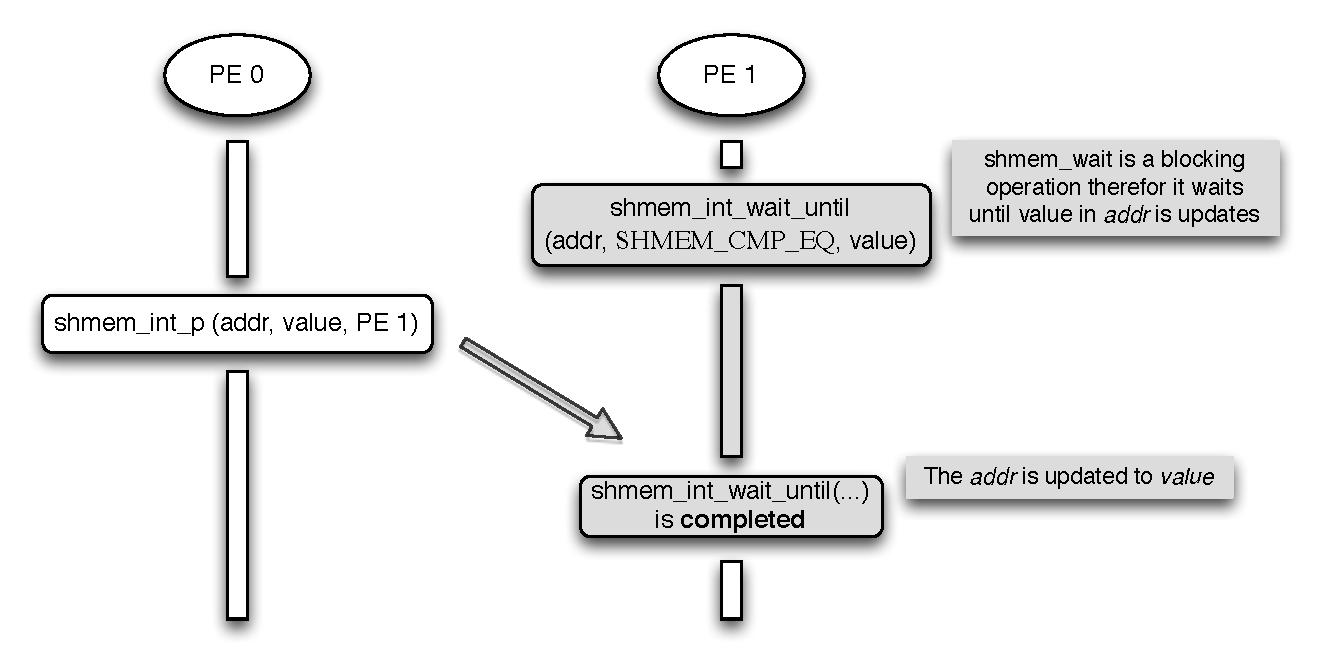
\includegraphics[width=0.7\textwidth]{diagrams/updated/wait}}
\end{tabular}

\begin{tabular}{p{0.2\textwidth} | p{0.7\textwidth}}
{}
&
{ Waits for a symmetric variable to be updated by a remote \ac{PE}. Should be used when computation on the local \ac{PE} cannot proceed without the value that the remote \ac{PE} is to update.} \tabularnewline
\hline 
\end{tabular}

\begin{tabular}{p{0.2\textwidth} | p{0.7\textwidth}}

{Ordering puts issued by a local \ac{PE}} \\
\FUNC{shmem\_fence} 
& 
\raisebox{-\totalheight}{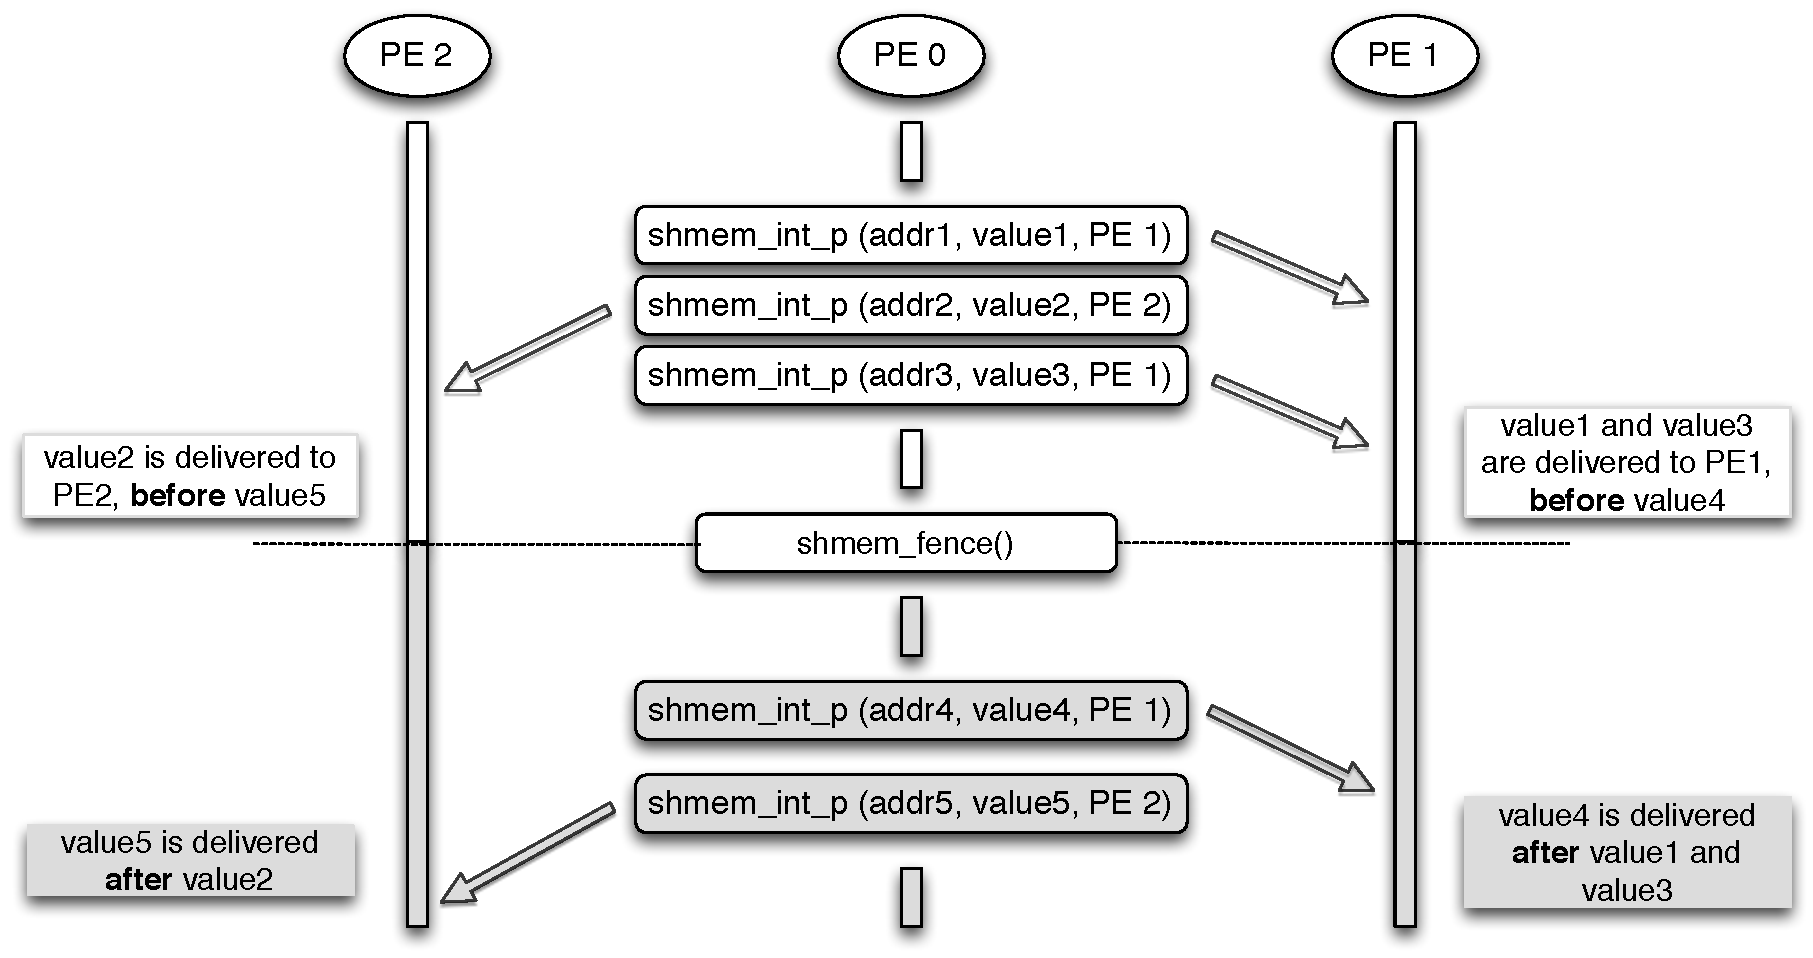
\includegraphics[width=0.7\textwidth]{diagrams/updated/fence}}
\end{tabular}

\begin{tabular}{p{0.2\textwidth} | p{0.7\textwidth}}
{}
&
All \PUT{} routines, \acp{AMO} and store routines on symmetric data issued to same \ac{PE}  are guaranteed to be delivered  before Puts (to the same \ac{PE}) issued after the \FUNC{fence} call. \tabularnewline
%Fence guaranteed order of puts before and after before \Put{}s 
%before the fence operation by the local \ac{PE} are guaranteed to be completed and visible before puts issued after the fence call.
% This operation should be used when all remote writes by a local \ac{PE} to a specific remote \ac{PE} need to be visible %(\rcomment{Swaroop: assuming visible == delivered}) 
%before any new remote write operation to the same \ac{PE}. \tabularnewline
\hline 
\end{tabular}

\begin{tabular}{p{0.2\textwidth} | p{0.7\textwidth}}
\hline 
\textbf{\openshmem  \ac{API}} & \centering \textbf{Working of \openshmem \ac{API}} \tabularnewline
\hline 
\hline
{Ordering puts issued by all \ac{PE} }\\
\FUNC{shmem\_quiet}
& 
\raisebox{-\totalheight}{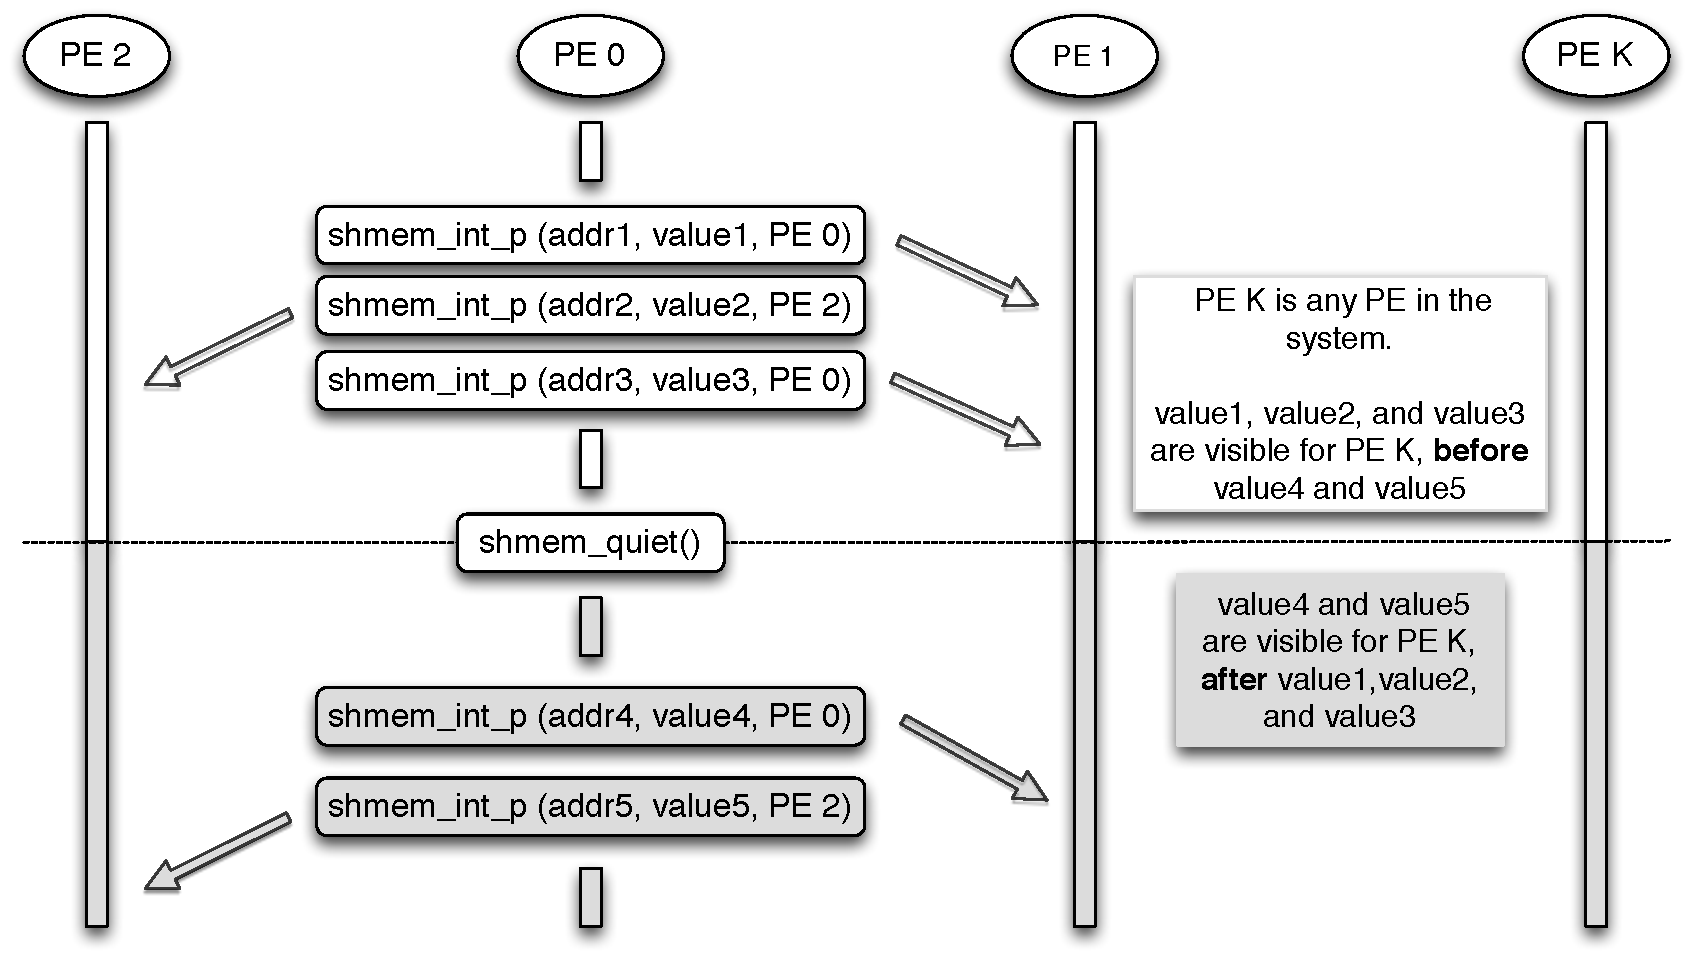
\includegraphics[width=0.7\textwidth]{diagrams/updated/quiet}} 
\end{tabular}

\begin{tabular}{p{0.2\textwidth} | p{0.7\textwidth}}
{}
&
{All \PUT{} routines, \acp{AMO} and store routines on symmetric data issued by a local \ac{PE} to all  remote \ac{PE}s are guaranteed to be completed and visible once quiet returns. This routine should be used when all remote writes issued by a local \ac{PE} need to be visible  to all other \ac{PE}s before the local \ac{PE} proceeds. } \tabularnewline
\hline 
\end{tabular}


\begin{tabular}{p{0.2\textwidth} | p{0.7\textwidth}}
Collective synchronization over an \activeset \\
\FUNC{shmem\_barrier}
&  
\raisebox{-\totalheight}{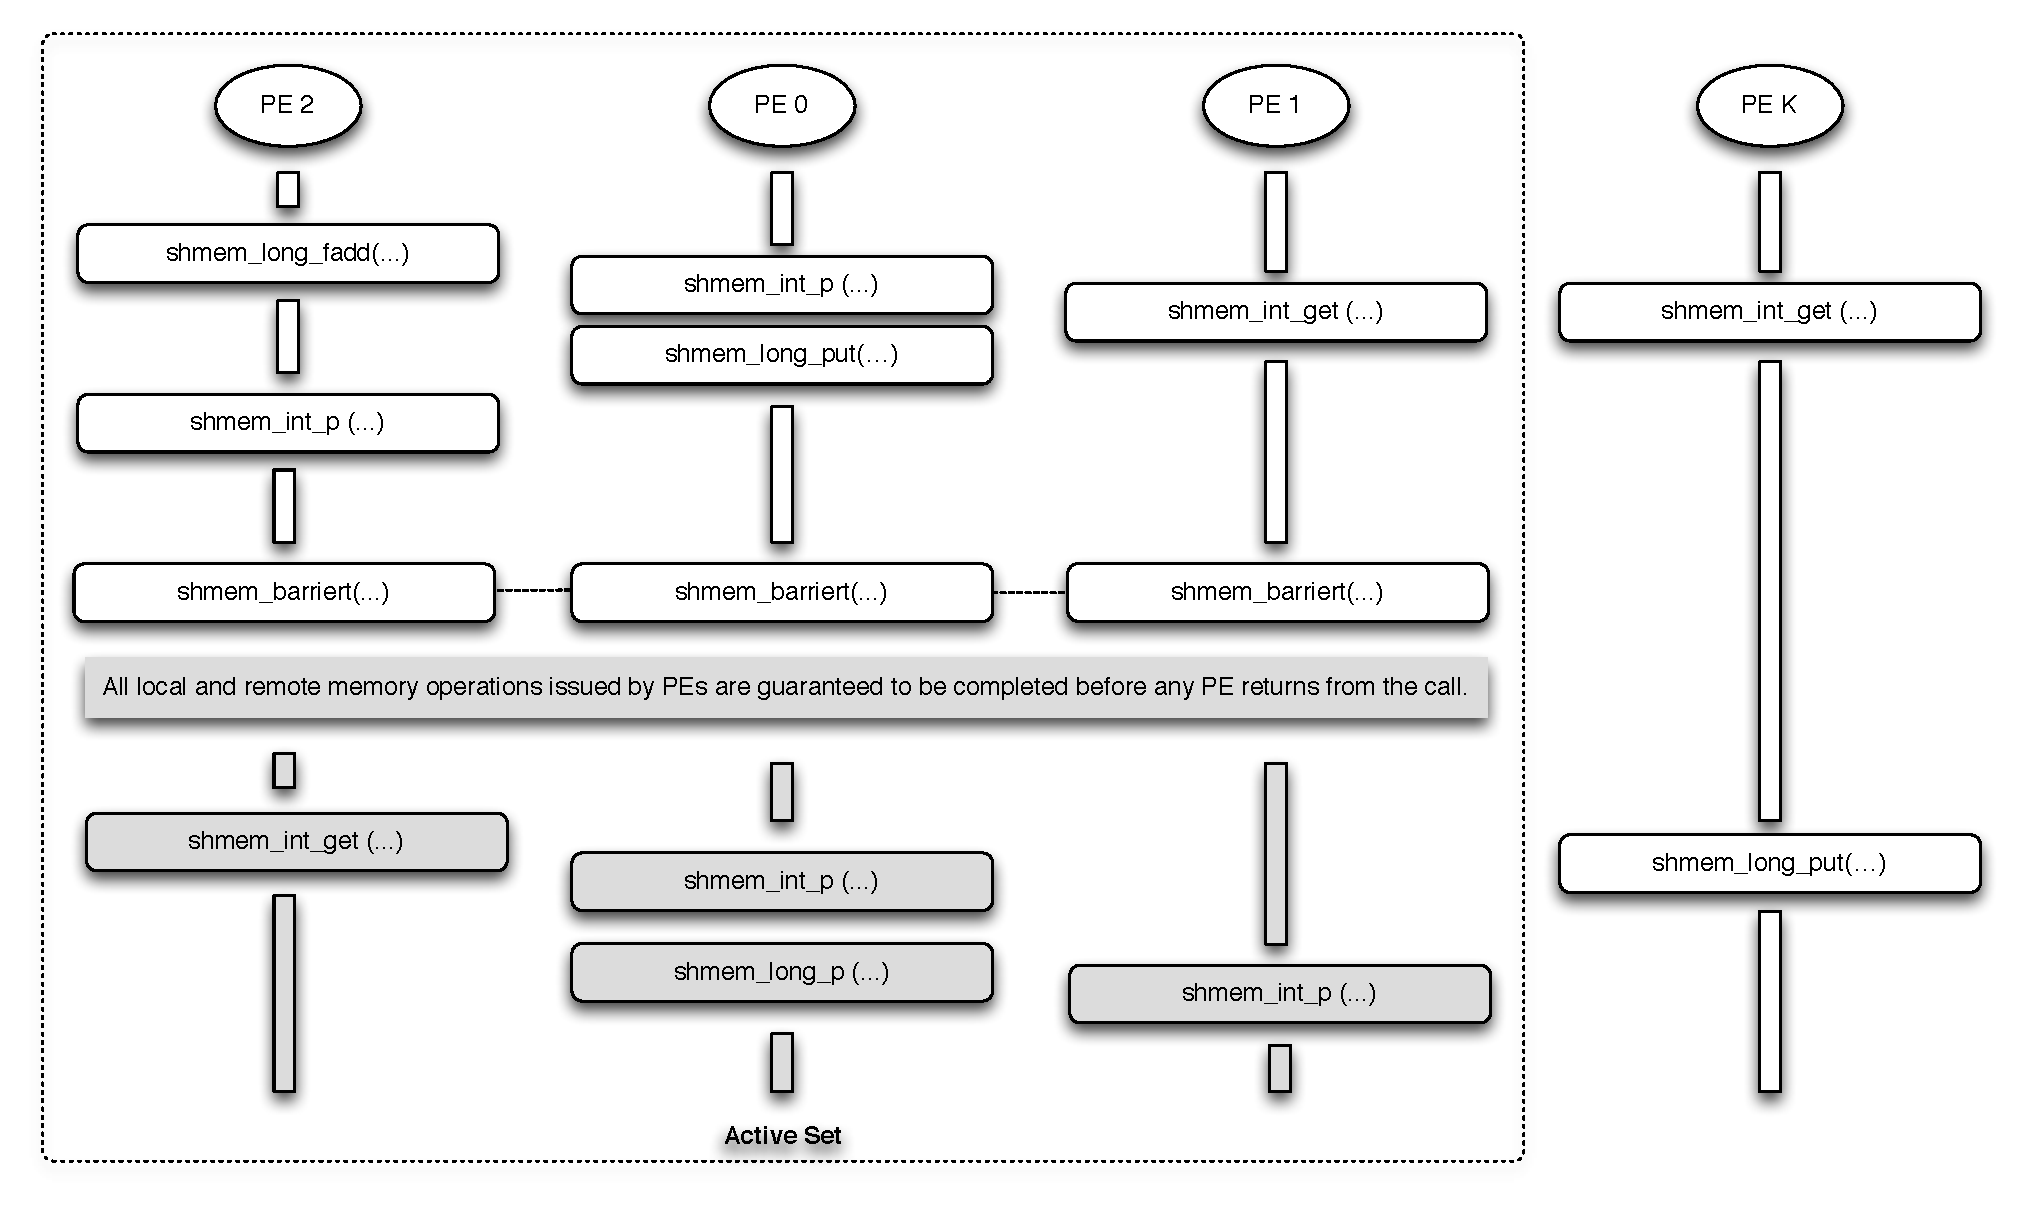
\includegraphics[width=0.7\textwidth]{diagrams/updated/barrier}} 
\end{tabular}

\begin{tabular}{p{0.2\textwidth} | p{0.7\textwidth}}
{}
&
{All local and remote memory operations issued by all \ac{PE}s within the \activeset{} are guaranteed to be completed before any \ac{PE} in the \activeset{} returns from the call. Additionally, no \ac{PE} my return from the barrier until all \ac{PE}s in the \activeset{} have entered the same barrier call. This routine should be used when synchronization as well as completion of all stores and remote memory updates via \openshmem is required over a sub set of the executing \ac{PE}s.} \tabularnewline %Figure (\ref{fig:barrier}).
\hline 
\end{tabular}

\begin{tabular}{p{0.2\textwidth} | p{0.7\textwidth}}
\hline 
\textbf{\openshmem  \ac{API}} & \centering \textbf{Working of \openshmem \ac{API}} \tabularnewline
\hline 
\hline
{Collective synchronization over all \ac{PE}s} \\
 \FUNC{shmem\_barrier\_all}
& 
\raisebox{-\totalheight}{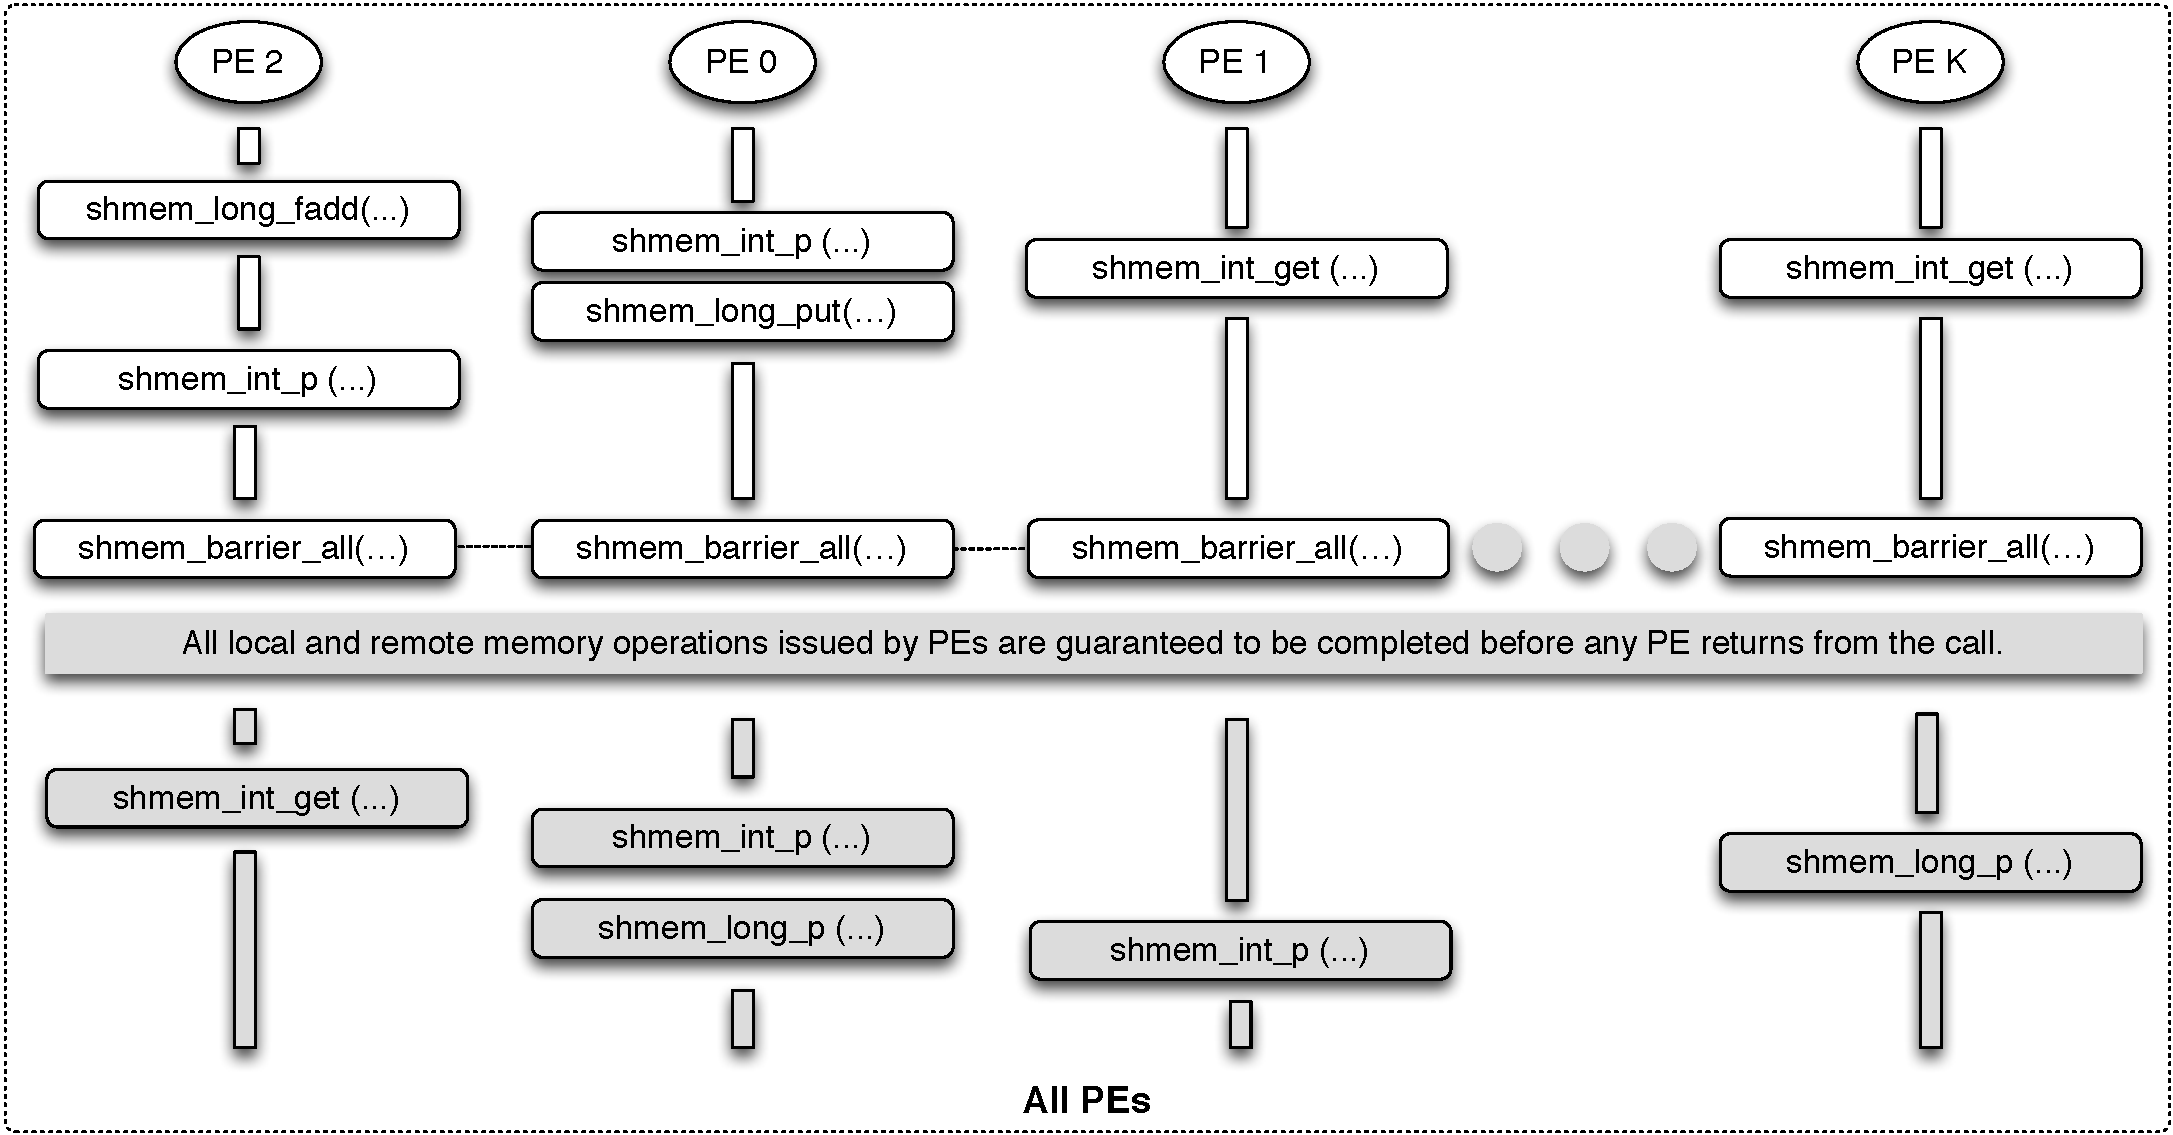
\includegraphics[width=0.7\textwidth]{diagrams/updated/barrierall}}
\end{tabular}

\begin{tabular}{p{0.2\textwidth} | p{0.7\textwidth}}
{}
&
{All local and remote memory operations issued by all \ac{PE}s are guaranteed to be completed before any \ac{PE} returns from the call. Additionally no \ac{PE} shall return from the barrier until all \ac{PE}s have entered the same \FUNC{shmem\_barrier\_all} call. This routine should be used when synchronization as well as completion of all stores and remote memory updates via \openshmem is required over all \ac{PE}s. } \tabularnewline
\hline 
\end{tabular}
\clearpage
%%%%%%%%%%%%%%%%%OLD LAYOUT%%%%%%%%%%%%%%%%
%\begin{tabular}{|p{0.2\textwidth}|p{0.4\textwidth}|p{0.3\textwidth}|}
%\hline 
%\textbf{\openshmem  \ac{API}} & \centering \textbf{Working of \openshmem \ac{API}} & \textbf{Appropriate Situation}\tabularnewline
%\hline 
%\hline 
%{Point-to-point synchronization}\\
%\FUNC{shmem\_wait}, \FUNC{shmem\_wait\_until} 
%&
%\raisebox{-\totalheight}{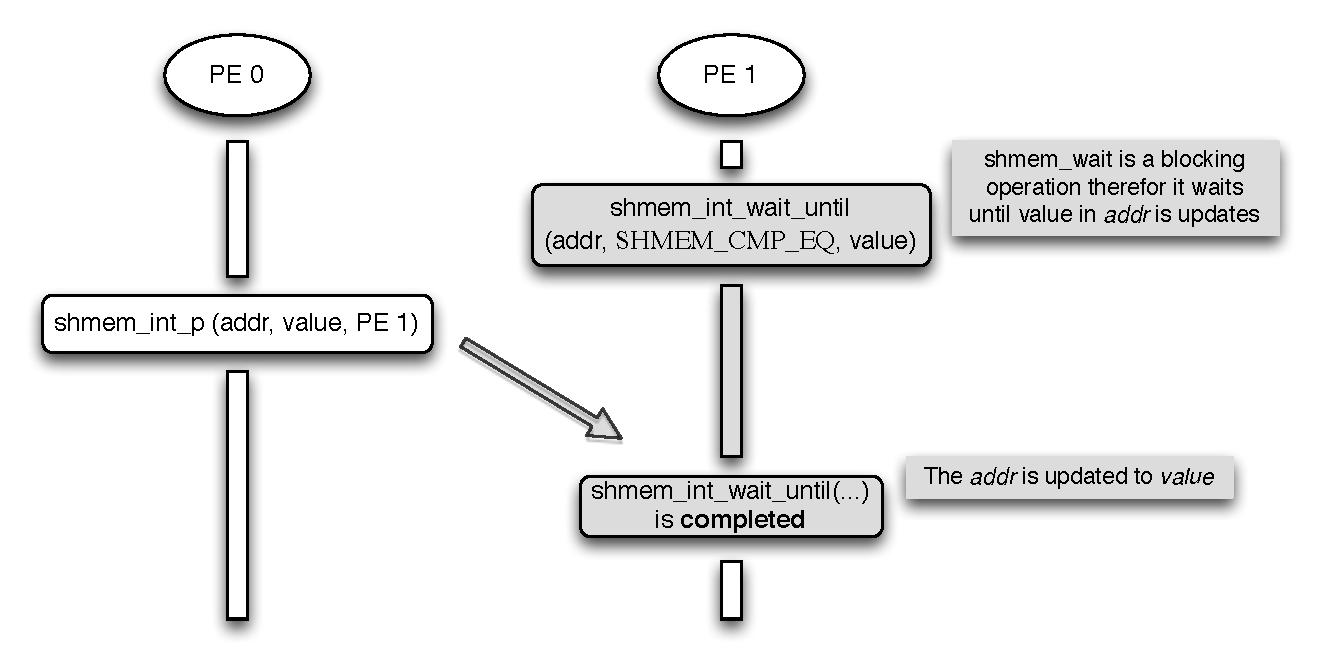
\includegraphics[width=0.39\textwidth]{diagrams/updated/wait}}
%{Waits for a symmetric variable to be updated by a remote \ac{PE}. Should be used when computation at the local \ac{PE} cannot proceed without the value that the remote \ac{PE} is to update.} \tabularnewline
%% Figure (\ref{fig:wait}).}\tabularnewline
%\hline 
%Ordering puts issued by a local \ac{PE} \\
%\FUNC{shmem\_fence} 
%& 
%\raisebox{-\totalheight}{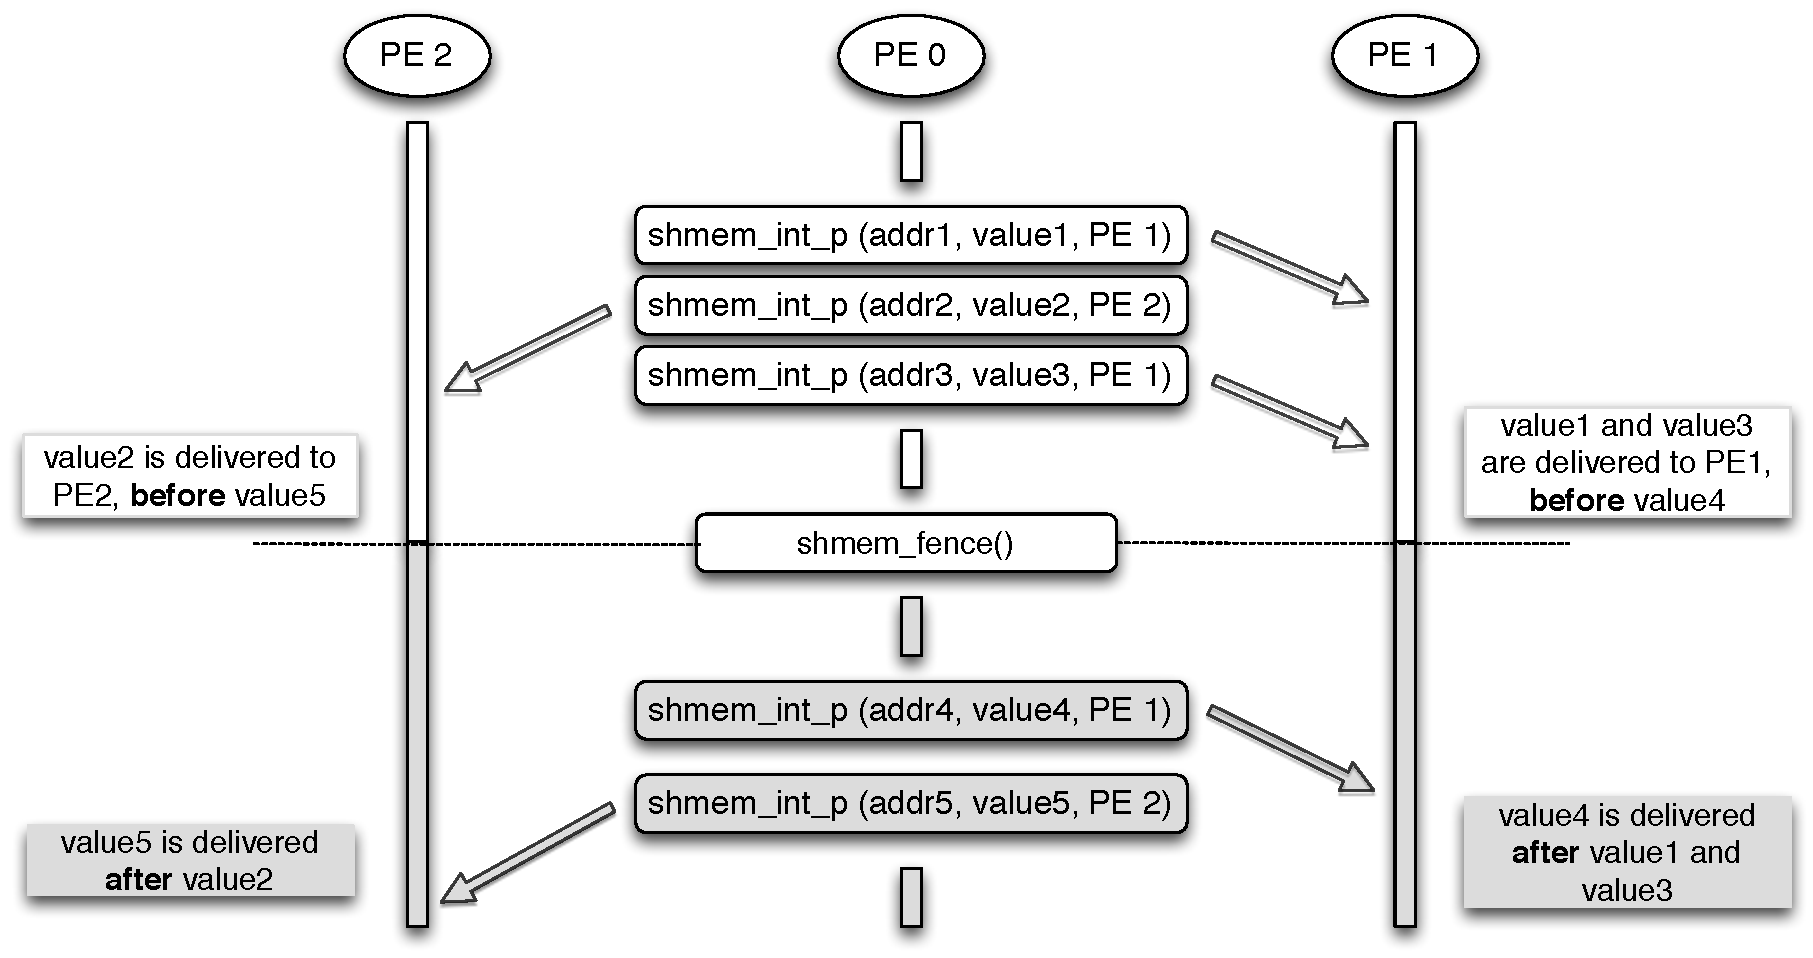
\includegraphics[width=0.39\textwidth]{diagrams/updated/fence}}
%& 
%All puts issued before the fence operation by the local \ac{PE} are guaranteed to be delivered before puts issued after the fence call to the same remote \ac{PE}. This operation should be used when all remote writes by a local \ac{PE} to a remote \ac{PE} need to be visible %(\rcomment{Swaroop: assuming visible == delivered}) 
%before any new remote write operation to the same \ac{PE}. \tabularnewline
%%Figure (\ref{fig:fence}).\tabularnewline
%\hline 
%Ordering puts issued by all \ac{PE} \\
%\FUNC{shmem\_quiet}
%& 
%\raisebox{-\totalheight}{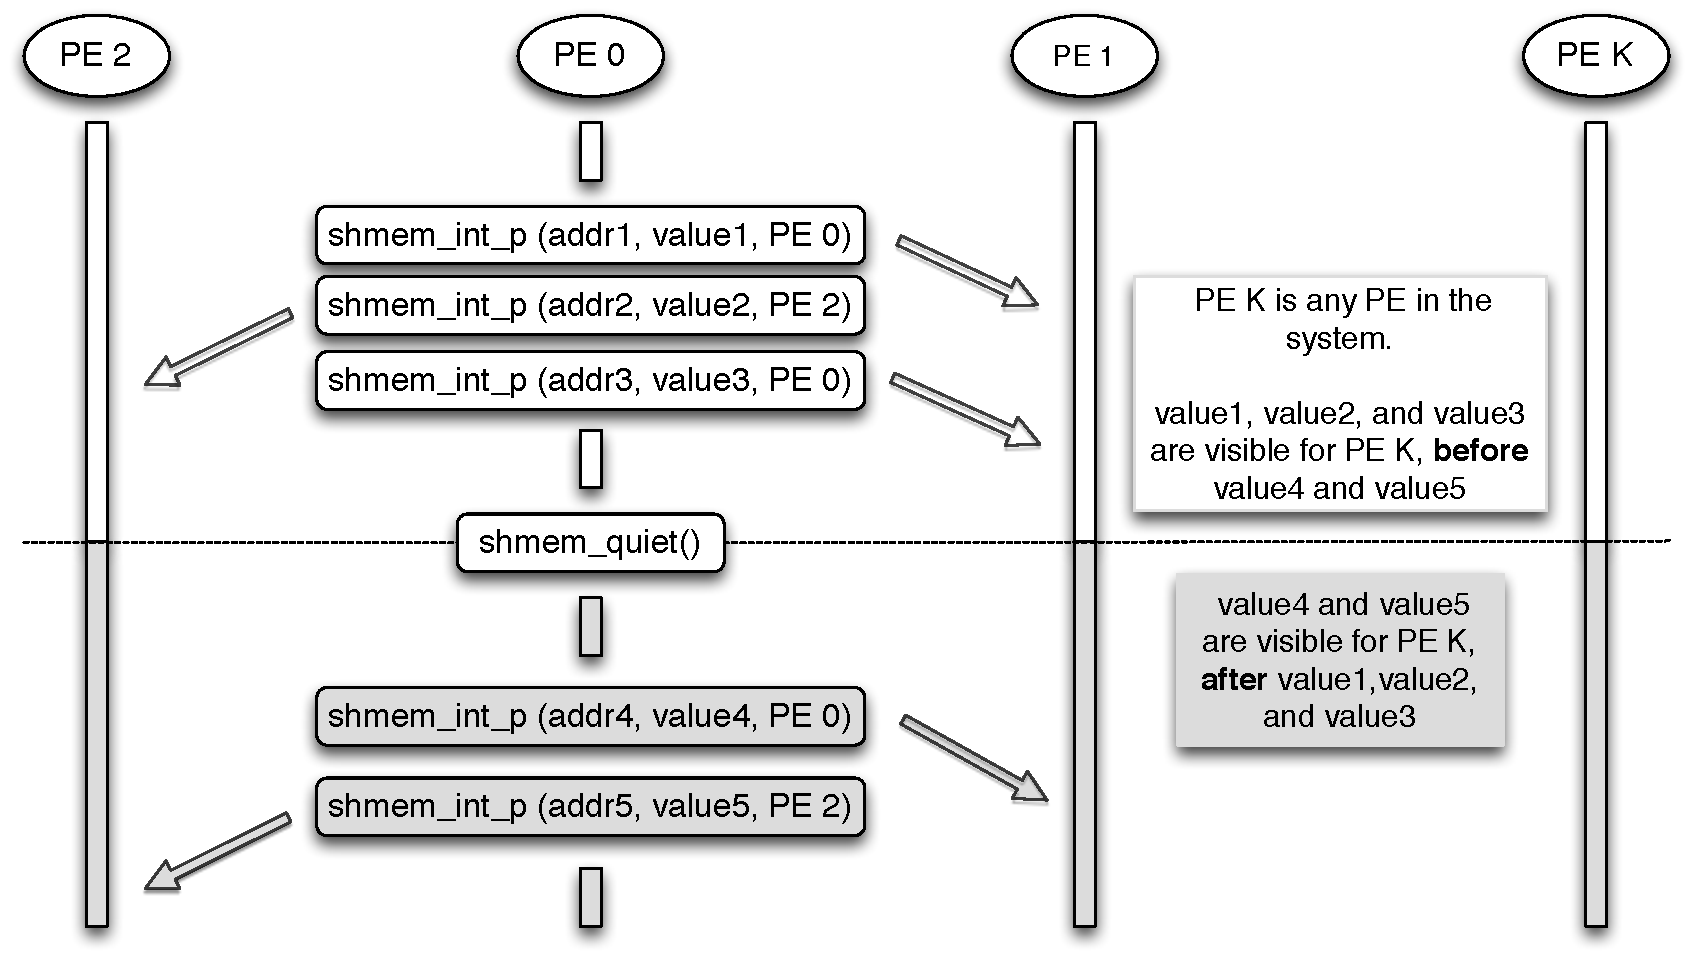
\includegraphics[width=0.39\textwidth]{diagrams/updated/quiet}} 
%& 
%{All puts issued by all \ac{PE}s are guaranteed to be delivered before the next local update or remote memory update via \openshmem (\rcomment{May change after SGI's input.}). This operation should be used when all remote writes by all \ac{PE}s need to be visible  to all other \ac{PE}s before any new local or remote memory update via \openshmem library operation. } \tabularnewline
%%Figure (\ref{fig:quiet}).} \tabularnewline
%\hline 
%\end{tabular}
%\clearpage
%\begin{tabular}{|p{0.2\textwidth}|p{0.4\textwidth}|p{0.3\textwidth}|}
%\hline 
%Collective synchronization over an \activeset \\
%\FUNC{shmem\_barrier}
%&  
%\raisebox{-\totalheight}{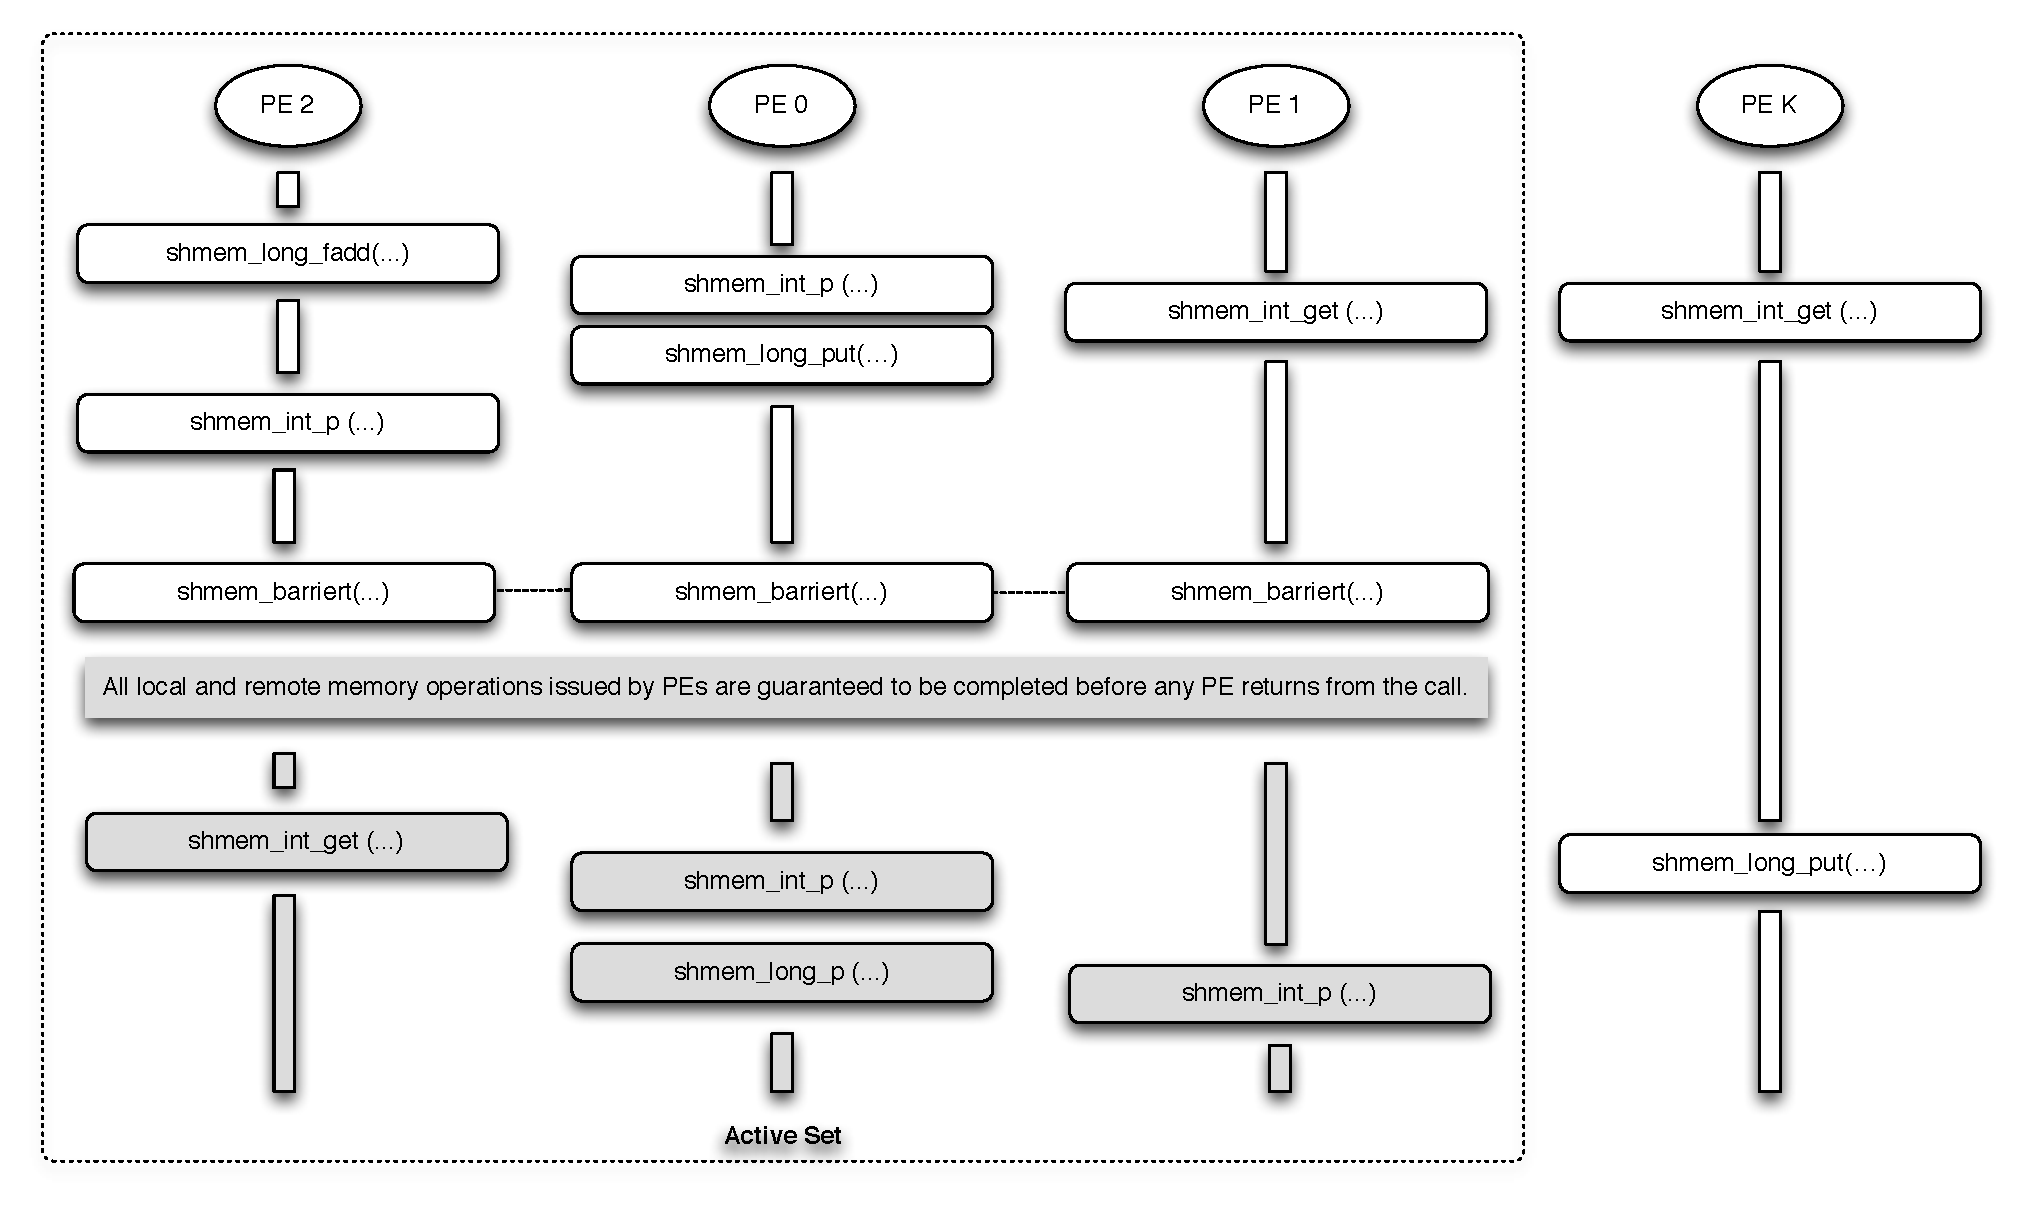
\includegraphics[width=0.39\textwidth]{diagrams/updated/barrier}} 
%& 
%{All local and remote memory operations issued by all \ac{PE}s within the \activeset{} are guaranteed to be completed before any \ac{PE} in the \activeset{} returns from the call. Additionally no \ac{PE} my return from the barrier till all \ac{PE}s in the \activeset{} have called the same barrier call. This operation should be used when synchronization as well as completion of local stores and remote memory updates via \openshmem is required over a sub-set of the executing \ac{PE}s.} \tabularnewline %Figure (\ref{fig:barrier}).
%\hline 
%Collective synchronization over all \ac{PE}s \\
% \FUNC{shmem\_barrier\_all}
%& 
%\raisebox{-\totalheight}{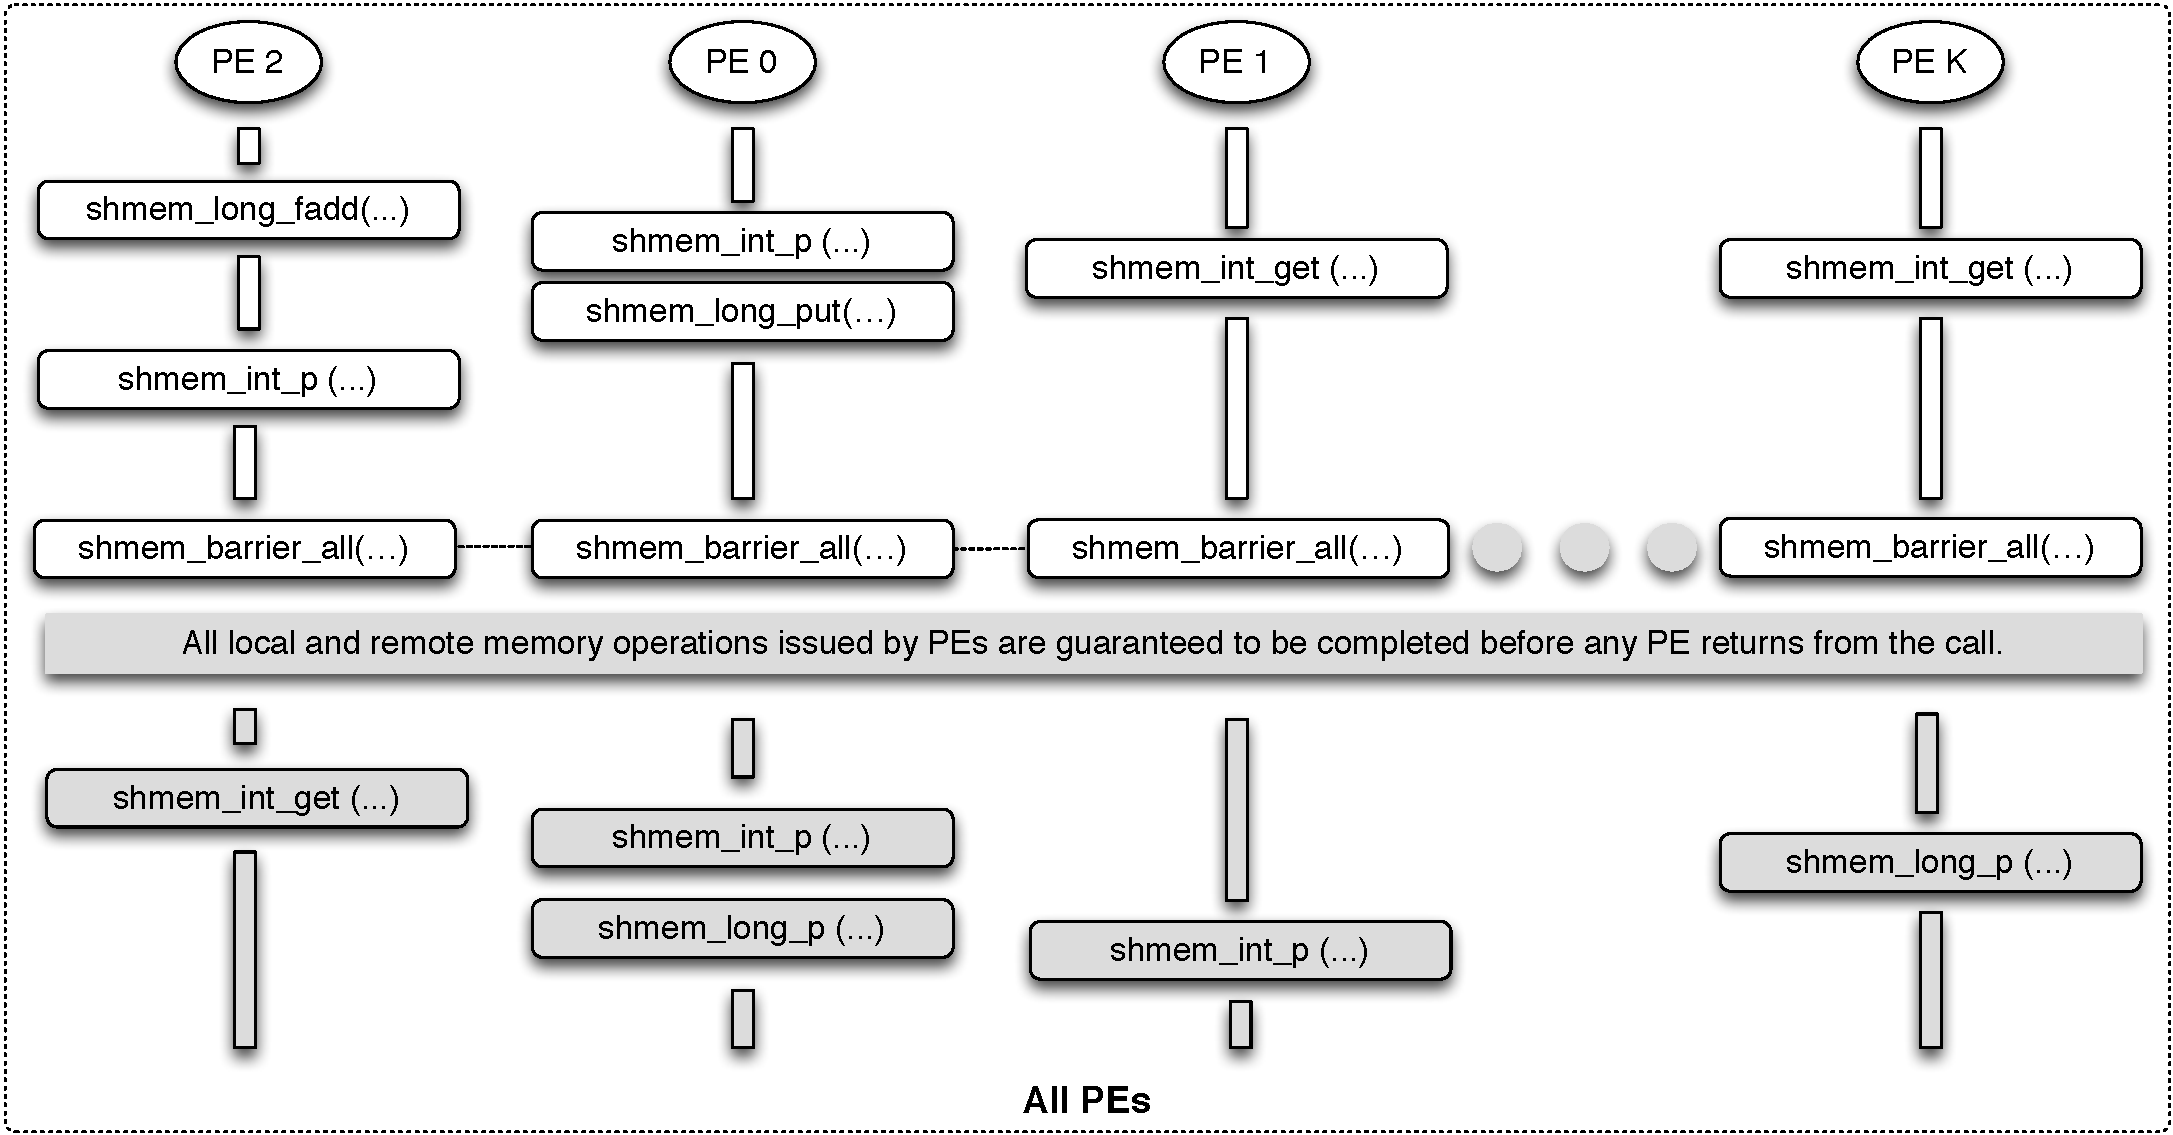
\includegraphics[width=0.39\textwidth]{diagrams/updated/barrierall}}
%& 
%{All local and remote memory operations issued by all \ac{PE}s are guaranteed to be completed before any \ac{PE} returns from the call. Additionally no \ac{PE} my return from the barrier until all \ac{PE}s have called the same barrier call. This operation should be used when synchronization as well as completion of local stores and remote memory updates via \openshmem is required over all \ac{PE}s. } \tabularnewline%Figure (\ref{fig:barrierall}).
%
%\hline 
%\end{tabular}


%\begin{figure}
%%        \centering
%        \begin{subfigure}{0.5\textwidth}
%                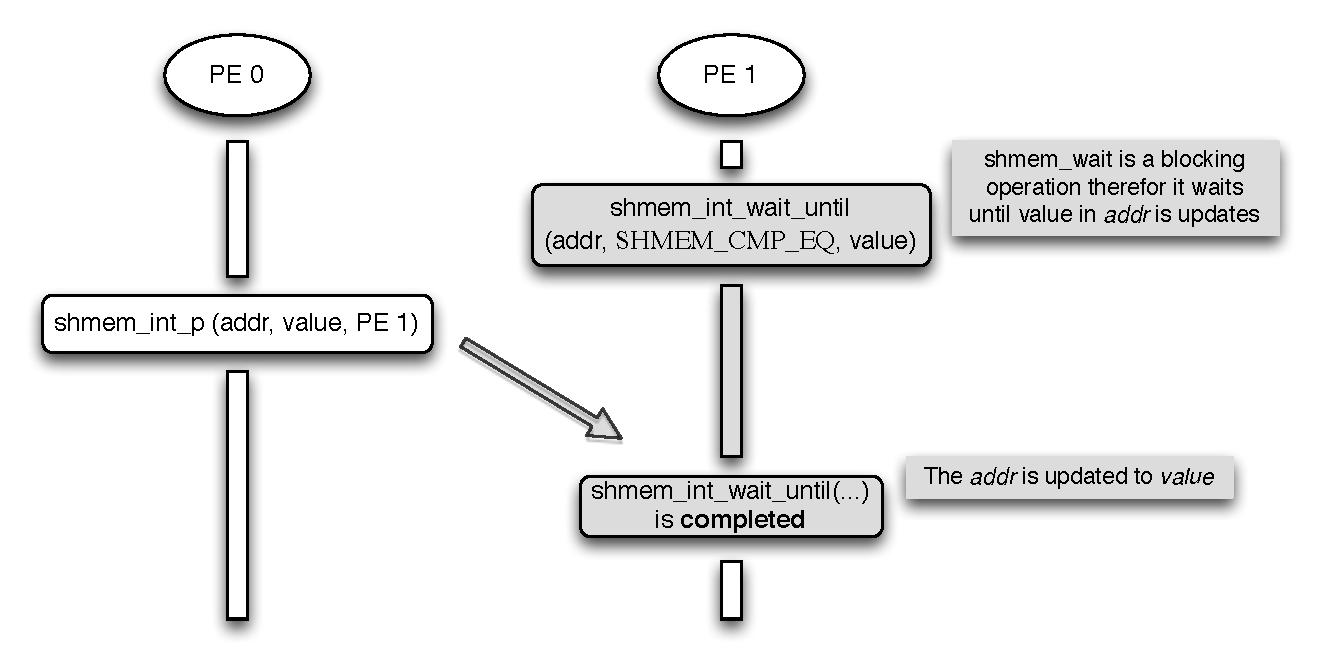
\includegraphics[width=\textwidth]{diagrams/updated/wait}
%                \caption{\FUNC{shmem\_wait}}
%                \label{fig:wait}
%        \end{subfigure}
%        \begin{subfigure}{0.49\textwidth}
%                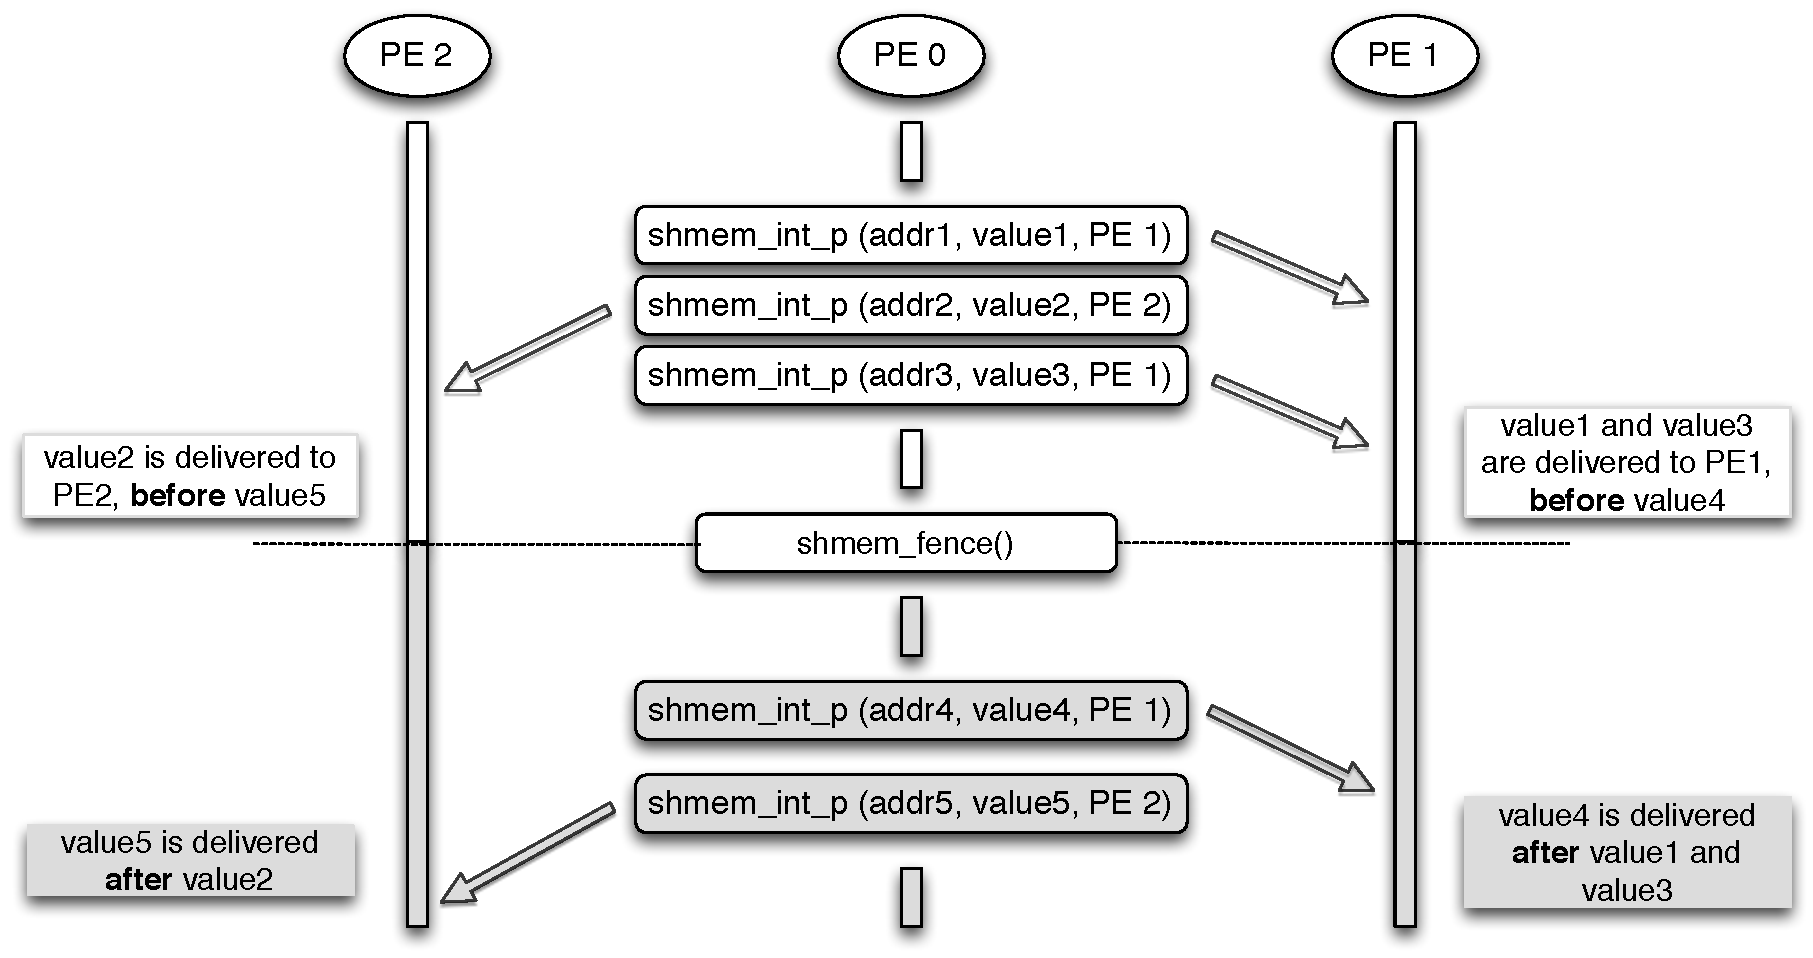
\includegraphics[width=\textwidth]{diagrams/updated/fence}
%                \caption{\FUNC{shmem\_fence}}
%                \label{fig:fence}
%        \end{subfigure}
%        \begin{subfigure}{0.48\textwidth}
%                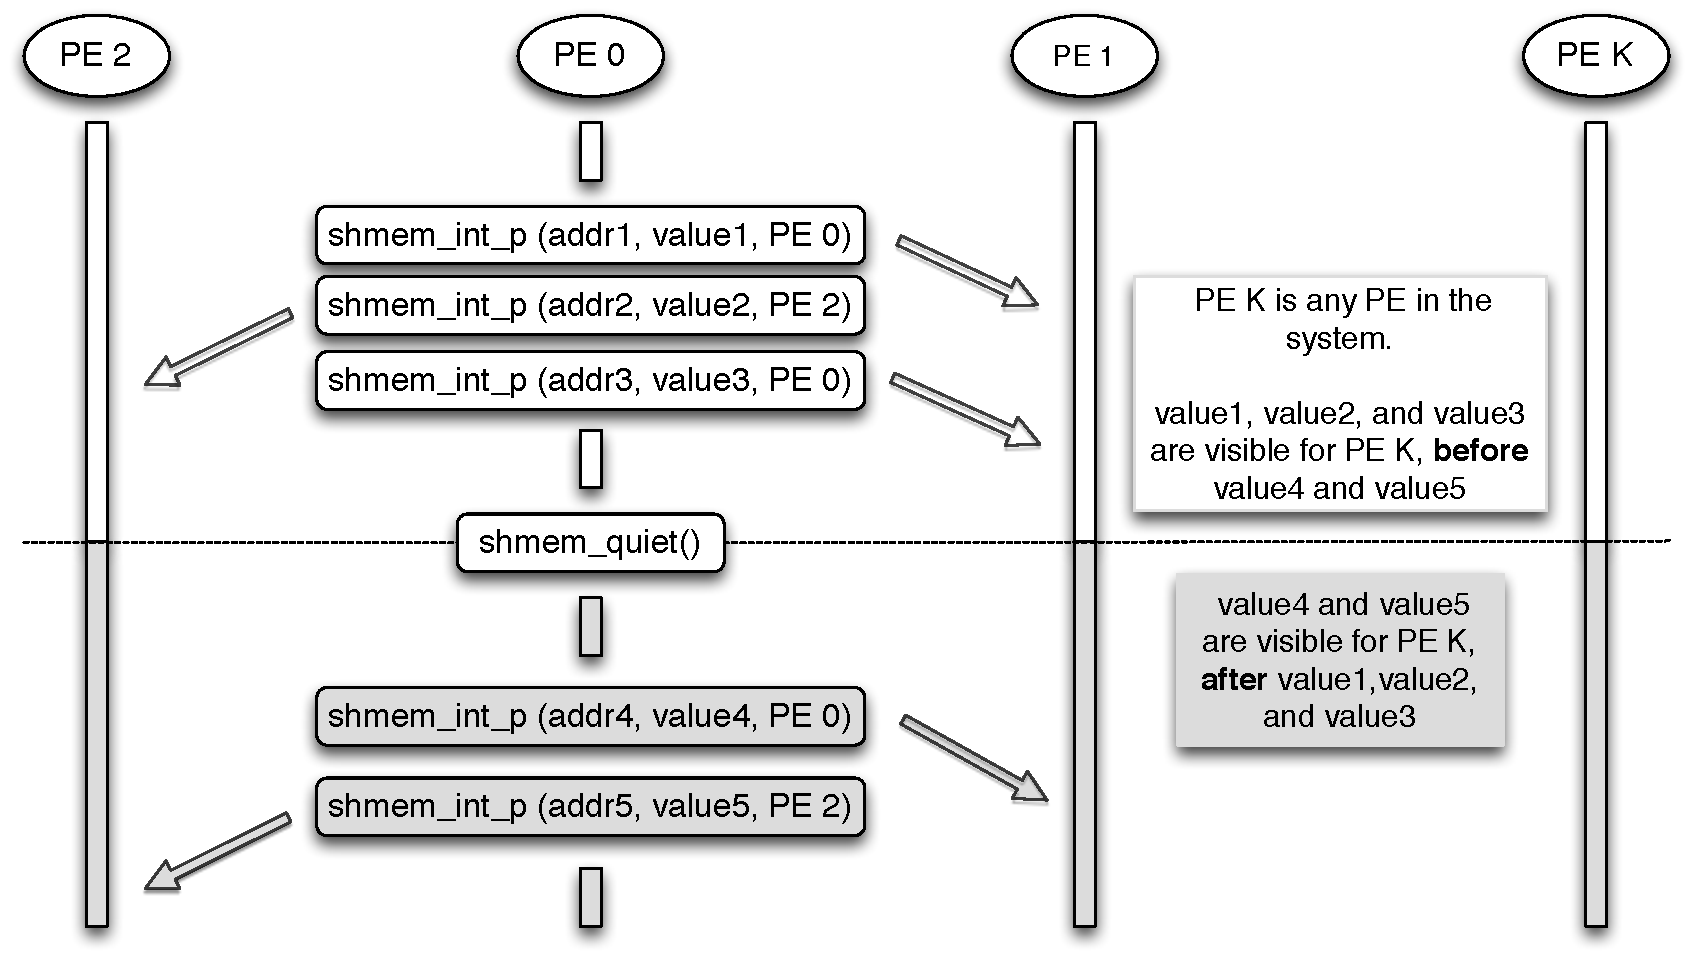
\includegraphics[width=\textwidth]{diagrams/updated/quiet}
%                \caption{\FUNC{shmem\_quiet}}
%                \label{fig:quiet}
%        \end{subfigure}
%	    \begin{subfigure}{0.48\textwidth}
%		        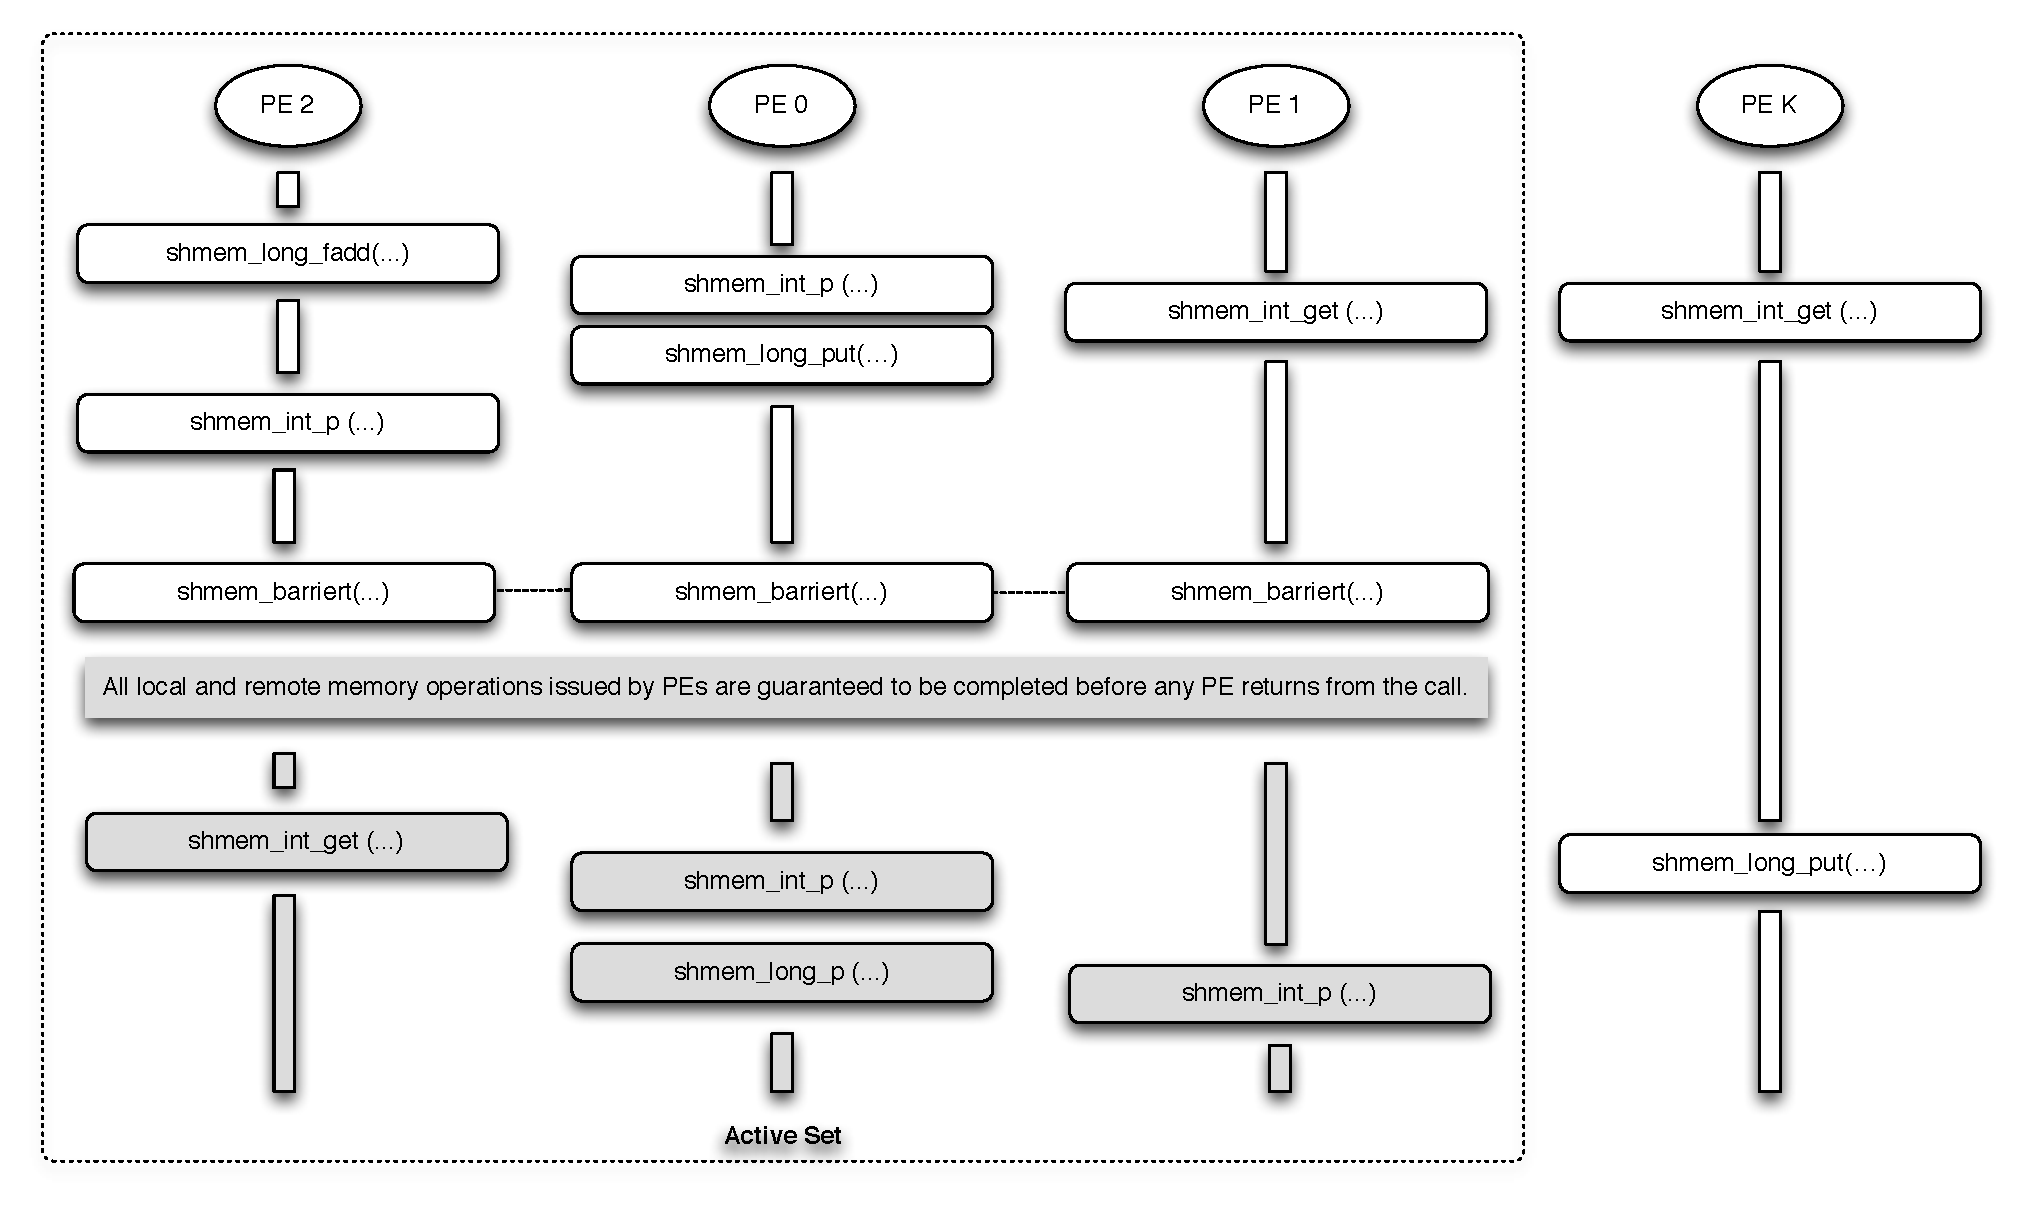
\includegraphics[width=\textwidth]{diagrams/updated/barrier}
%		        \caption{\FUNC{shmem\_barrier}}
%		\label{fig:barrier}
%	    \end{subfigure}
%        \centering
%	    \begin{subfigure}{0.48\textwidth}
%		        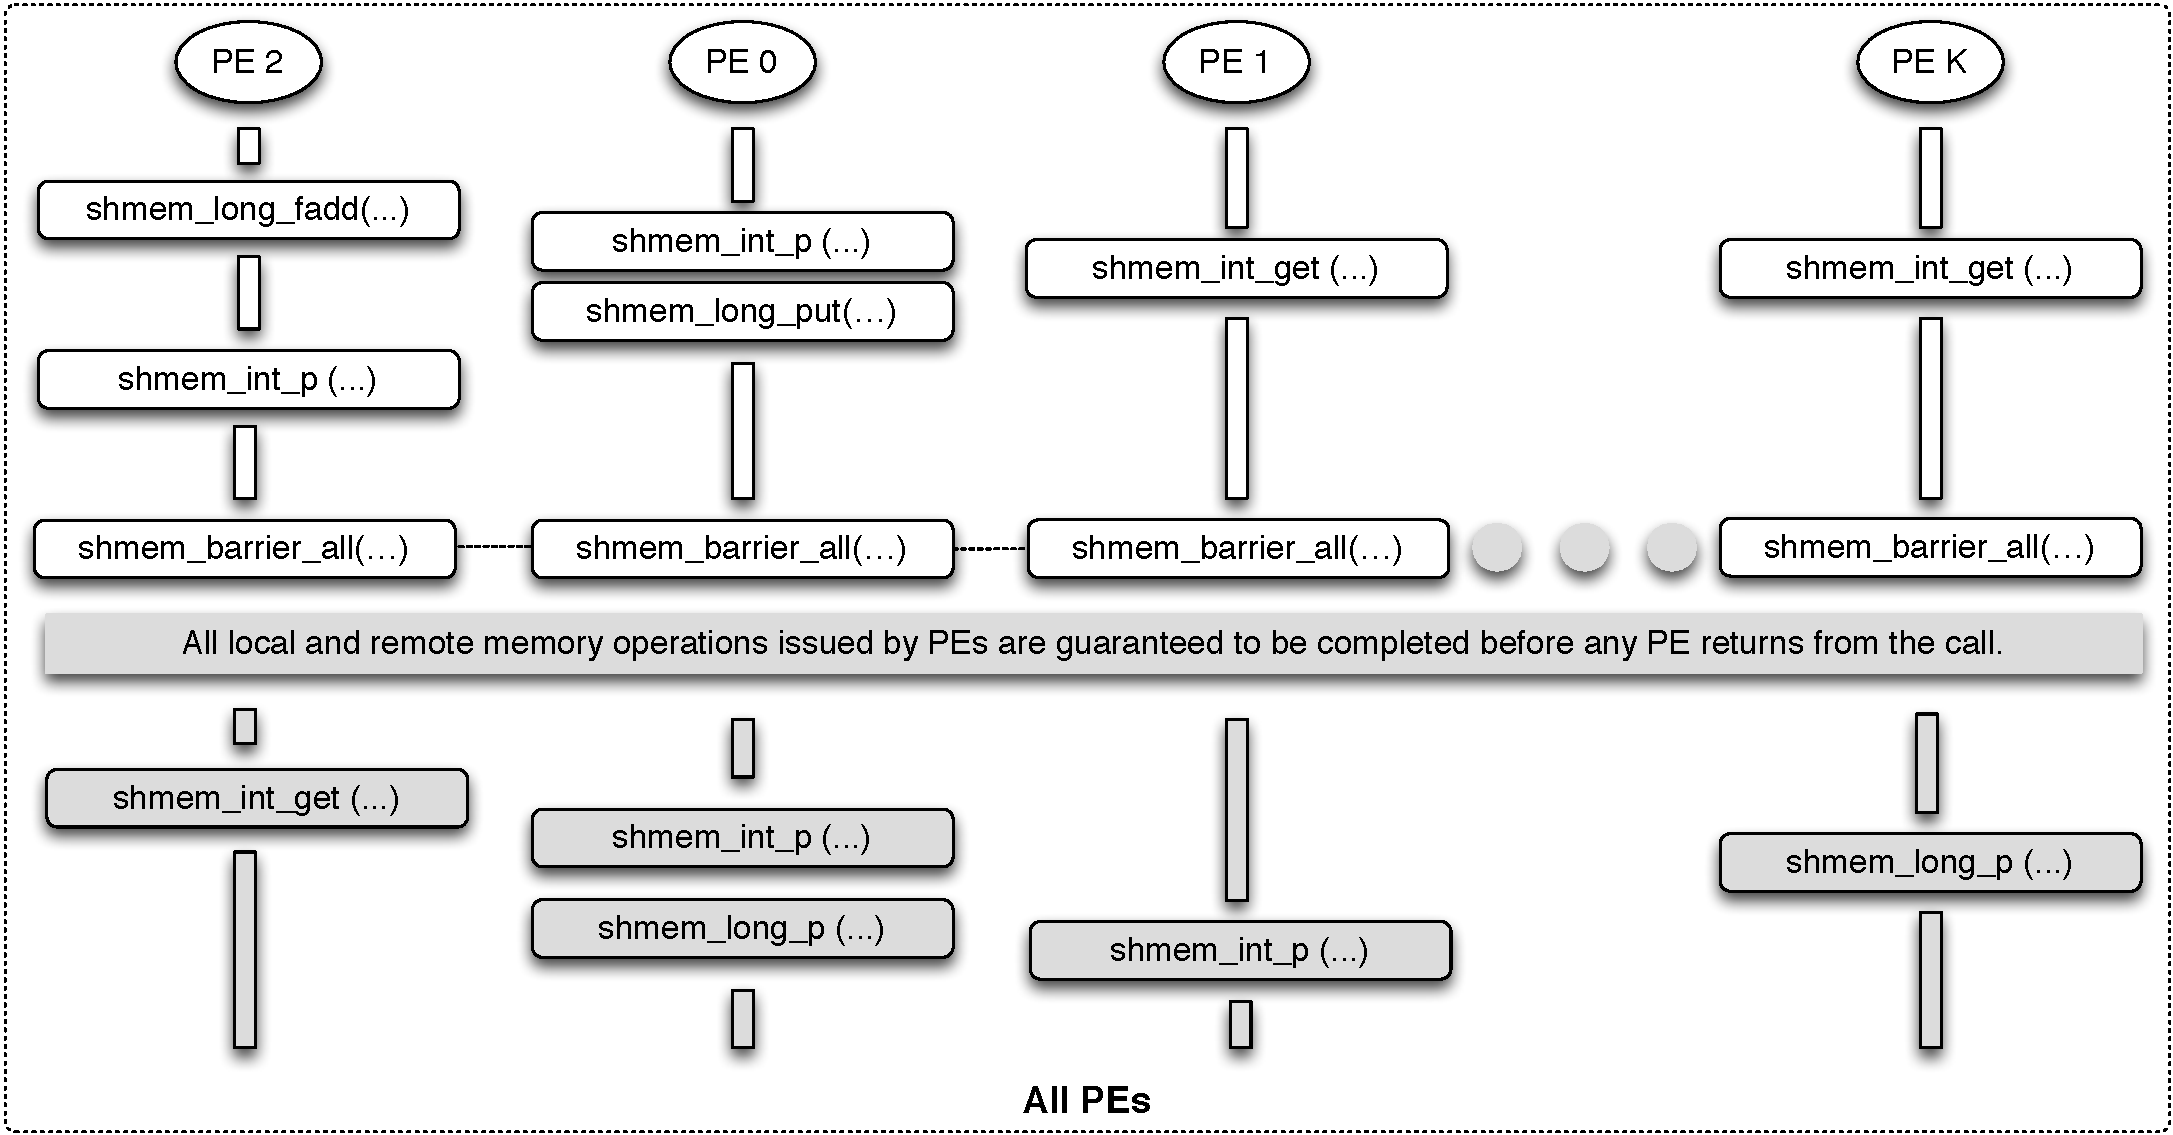
\includegraphics[width=\textwidth]{diagrams/updated/barrierall}
%		        \caption{\FUNC{shmem\_barrierall}}
%		\label{fig:barrierall}
%	    \end{subfigure}
%        \caption{\openshmem{} synchronization operations}\label{fig:animals}
%\end{figure}

\bAPI{SHMEM\_PUT}{The  put routines  provide  a method for copying data from a contiguous local data object to a data object on a specified \ac{PE}.}
\synC   %Synopisis for C API

void shmem_double_put(double target, const double *source, size_t len, int pe);
void shmem_float_put(float *target, const float *source, size_t len, int pe);
void shmem_int_put(int *target, const int *source, size_t len, int pe);
void shmem_long_put(long *target, const long *source, size_t len, int pe);
void shmem_longdouble_put(long double *target, const long double *source, size_t len,int pe);
void shmem_longlong_put(long long *target, const long long *source, size_t len, int pe);
void shmem_put32(void *target, const void *source, size_t len, int pe);
void shmem_put64(void *target, const void *source, size_t len, int pe);
void shmem_put128(void *target, const void *source, size_t len, int pe);
void shmem_putmem(void *target, const void *source, size_t len, int pe);
void shmem_short_put(short*target, const short*source, size_t len, int pe); %*\synCE    %DO NOT DELETE. THIS LINE IS NOT A COMMENT

\synF   %Synopsis for FORTRAN API

CALL SHMEM_CHARACTER_PUT(target, source, len, pe)
CALL SHMEM_COMPLEX_PUT(target, source, len, pe)
CALL SHMEM_DOUBLE_PUT(target, source, len, pe)
CALL SHMEM_INTEGER_PUT(target, source, len, pe)
CALL SHMEM_LOGICAL_PUT(target, source, len, pe)
CALL SHMEM_PUT(target, source, len, pe)
CALL SHMEM_PUT4(target, source, len, pe)
CALL SHMEM_PUT8(target, source, len, pe)
CALL SHMEM_PUT32(target, source, len, pe)
CALL SHMEM_PUT64(target, source, len, pe)
CALL SHMEM_PUT128(target, source, len, pe)
CALL SHMEM_PUTMEM(target, source, len, pe)
CALL SHMEM_REAL_PUT(target, source, len, pe) %*\synFE   %DO NOT DELETE. THIS LINE IS NOT A COMMENT  

% Arguments table. If no arguments you can use \argRow{None}{}{} 
\desB{  
       \argRow{IN}{target}{Data object to be updated on the remote \ac{PE}. This data object must be remotely accessible.}
       \argRow{OUT}{source}{Data object containing the data to be copied.}
       \argRow{IN}{len}{Number of elements in the \VAR{target} and \VAR{source} arrays. \VAR{len} must be of type integer. If you are using \Fortran, it must be a constant, variable, or array element of default integer type.}
        \argRow{IN}{pe}{\ac{PE} number of the remote \ac{PE}. \VAR{pe} must be of type integer. If you are using \Fortran, it must be a constant, variable, or array element of default integer type.}
 }
 %API description
 {   The  routines  return  after the data has been copied out of the source
       array on the local \ac{PE}.
       The delivery of data words into the data object on the  destination \ac{PE}
       may  occur  in  any order.  Furthermore, two successive put operations
       may deliver  data  out  of  order  unless  a  call  to \FUNC{shmem\_fence}  is
       introduced between the two calls.   
 }
 %API Description Table. 
{
 % If there is no Description Table and return, this field can be 
 \hfill \\
  \desTB { 
    The  target  and source data  objects must conform to certain typing
    constraints, which are as follows: } 
    {
       \cRow{shmem\_putmem}{ \Fortran:  Any noncharacter type. \Clang:	 Any data  type.   len	is  scaled  in bytes.} 
       \cRow{shmem\_put4, shmem\_put32}{Any  noncharacter type that has a storage size equal to \CONST{32} bits. }
       \cRow{shmem\_put4, shmem\_put32}{Any  noncharacter type that has a storage size equal to \CONST{32} bits.}
       \cRow{shmem\_put8,  shmem\_put64}{Any noncharacter type that has a  storage size equal to \CONST{64} bits.}
       \cRow{shmem\_put8,  shmem\_put64}{Any noncharacter type that has a  storage size equal to \CONST{64} bits. }
       \cRow{shmem\_put128}{Any  noncharacter type that has a storage size equal to \CONST{128} bits. }
       \cRow{shmem\_double\_put}{Elements of type double.}
       \cRow{shmem\_longdouble\_put}{Elements of type long double.}
       \cRow{SHMEM\_CHARACTER\_PUT}{Elements of type character.  \VAR{len} is  the number  of	 characters to transfer. The actual character lengths of the source and target variables are ignored. }
       \cRow{SHMEM\_COMPLEX\_PUT}{Elements of type complex of default size.}
       \cRow{SHMEM\_DOUBLE\_PUT}{Elements of type double precision. }
       \cRow{SHMEM\_INTEGER\_PUT}{Elements of type integer.}
       \cRow{SHMEM\_LOGICAL\_PUT}{Elements of type logical.}
       \cRow{SHMEM\_REAL\_PUT}{Elements of type real.}
      } 
 %Return Values     
\desR{None.}

% Notes. If there are no notes, this field can be left empty.
\notesB{    If you are using \Fortran, data types must  be  of  default  size.   For
       example, a  real  variable  must  be  declared as  \CONST{REAL},  \CONST{REAL*4},  or
       \CONST{REAL(KIND=4)}.       
}
}%end of DesB
%Example
\exampleB{
%For each example, you can enter it as an item.
                  \exampleITEM
                  { The following \FUNC{shmem\_put} example is for  programs:}
                 {./EXAMPLES/shmem_put_example.c}
                 {} 
                 }  	
\eAPI 
 %Oscar
\bAPI{SHMEM\_P}{Copies one data item to a remote \ac{PE}.}
\synC 
void shmem_char_p(char *addr, char value, int pe);
void shmem_short_p(short *addr, short value, int pe);
void shmem_int_p(int *addr, int value, int pe);
void shmem_long_p(long *addr, long value, int pe);
void shmem_longlong_p(long long *addr, long long value, int pe);
void shmem_float_p(float *addr, float value, int pe);
void shmem_double_p(double *addr, double value, int pe);
void shmem_longdouble_p(long double *addr, long double value, int pe); %*\synCE    %DO NOT DELETE. THIS LINE IS NOT A COMMENT

\desB{
   \argRow{IN}{addr}{The remotely accessible array element or scalar data object
		 which will receive the data on the remote \ac{PE}.}
   \argRow{IN}{value}{The value to be transferred to \VAR{addr} on the remote \ac{PE}.}
   \argRow{IN}{pe}{The number of the remote \ac{PE}.}
}
{     These routines provide a very low latency  put  capability  for single
       elements of most basic types.

       As with \FUNC{shmem\_put}, these functions start the remote transfer and may
       return	before the   data  is delivered  to the  remote \ac{PE}.  Use
       \FUNC{shmem\_quiet} to force completion of all remote \FUNC{PUT} transfers.
}
{
\desR{None.}
\notesB{None.}
}
\exampleB {
\exampleITEM{The  following  simple  example	uses  \FUNC{shmem\_double\_p}  in a \Clang{} program.}	 
    	               {./EXAMPLES/shmem_p_example.c}{}
	               }
\eAPI
 %Oscar
\bAPI{SHMEM\_IPUT}{Copies  strided  data to  a specified processing element (PE).}
\synC
	  void	shmem_double_iput(double  *target,   const   double   *source,
	  ptrdiff_t tst, ptrdiff_t sst, size_t nelems, int pe);
	  void	shmem_float_iput(float *target, const float *source, ptrdiff_t
	  tst, ptrdiff_t sst, size_t nelems, int pe);
	  void shmem_int_iput(int *target, const int *source,  ptrdiff_t  tst,
	  ptrdiff_t sst, size_t nelems, int pe);
	  void	shmem_iput32(void  *target, const void *source, ptrdiff_t tst,
	  ptrdiff_t sst, size_t nelems, int pe);
	  void shmem_iput64(void *target, const void *source,  ptrdiff_t  tst,
	  ptrdiff_t sst, size_t nelems, int pe);
	  void	shmem_iput128(void *target, const void *source, ptrdiff_t tst,
	  ptrdiff_t sst, size_t nelems, int pe);
	  void shmem_long_iput(long *target,  const  long  *source,  ptrdiff_t
	  tst, ptrdiff_t sst, size_t nelems, int pe);
	  void	shmem_longdouble_iput(long  double  *target, const long double
	  *source, ptrdiff_t tst, ptrdiff_t sst, size_t nelems, int pe);
	  void shmem_longlong_iput(long long *target, const long long *source,
	  ptrdiff_t tst, ptrdiff_t sst, size_t nelems, int pe);
	  void	shmem_short_iput(short *target, const short *source, ptrdiff_t
	  tst, ptrdiff_t sst, size_t nelems, int pe);
%*\synCE    %DO NOT DELETE. THIS LINE IS NOT A COMMENT

\synF   %Synopsis for FORTRAN API
	  INTEGER tst, sst, nelems, pe
	  CALL SHMEM_COMPLEX_IPUT(target, source, tst, sst, nelems, pe)
	  CALL SHMEM_DOUBLE_IPUT(target, source, tst, sst, nelems, pe)
	  CALL SHMEM_INTEGER_IPUT(target, source, tst, sst, nelems, pe)
	  CALL SHMEM_IPUT4(target, source, tst, sst, nelems, pe)
	  CALL SHMEM_IPUT8(target, source, tst, sst, nelems, pe)
	  CALL SHMEM_IPUT32(target, source, tst, sst, nelems, pe)
	  CALL SHMEM_IPUT64(target, source, tst, sst, nelems, pe)
	  CALL SHMEM_IPUT128(target, source, tst, sst, nelems, pe)
	  CALL SHMEM_LOGICAL_IPUT(target, source, tst, sst, nelems, pe)
	  CALL SHMEM_REAL_IPUT(target, source, tst, sst, nelems, pe)
%*\synFE   %DO NOT DELETE. THIS LINE IS NOT A COMMENT  

\desB{
\argRow{OUT}{target}{Array to be updated on the remote PE.	This data object  must
		 be remotely accessible.}
\argRow{IN}{source}{Array containing the data to be copied.}
\argRow{IN}{tst}{The  stride between consecutive elements of the target array.
		 The stride is scaled by the element size of the target array.
		 A  value of 1 indicates contiguous data.  tst must be of type
		 integer.  If you are using Fortran,  it must	be  a  default
		 integer value.}
\argRow{IN}{sst}{The  stride between consecutive elements of the source array.
		 The stride is scaled by the element size of the source array.
		 A  value of 1 indicates contiguous data.  sst must be of type
		 integer.  If you are using Fortran,  it  must	be  a  default
		 integer value.}
\argRow{IN}{nelems}{Number of elements in the target and source arrays.  nelems must
		 be of type integer.  If you are using Fortran, it must	 be  a
		 constant, variable, or array element of default integer type.}
\argRow{IN}{pe}{PE number of the remote PE.  pe must be of type integer.   If
		 you  are  using  Fortran, it must be a constant, variable, or
		 array element of default integer type.}
}
{

       The iput routines provide  a method  for  copying 
       strided data elements of an array  from  the  local PE  to strided locations 
       of a symmetric array on a different PE.  The routines return when the data has been copied out of
       the  source  array  on the local PE but not necessarily before the data
       has been delivered to the remote data object.
}
{
    \desTB{
       The target and source data objects must conform to typing  constraints,
       which are as follows:}
      {
     \cRow{shmem\_iput32, shmem\_iput4}{Any  noncharacter type that has a storage
				     size equal to 32 bits.}
     \cRow{shmem\_iput64, shmem\_iput8}{Any noncharacter type that has a  storage
				     size equal to 64 bits.}
     \cRow{shmem\_iput128}{Any  noncharacter type that has a storage
				     size equal to 128 bits.}
     \cRow{shmem\_short\_iput}{Elements of type short.}
     \cRow{shmem\_int\_iput}{Elements of type short.}
     \cRow{shmem\_long\_iput}{Elements of type long.}
     \cRow{shmem\_longlong\_iput}{Elements of type long long.}
     \cRow{shmem\_float\_iput}{Elements of type float.}
     \cRow{shmem\_double\_iput}{Elements of type float.}
     \cRow{shmem\_longdouble\_iput}{Elements of type long double.}
     \cRow{SHMEM\_COMPLEX\_IPUT}{Elements of type complex of default size.}
     \cRow{SHMEM\_DOUBLE\_IPUT}{Elements of type double precision.}
     \cRow{SHMEM\_INTEGER\_IPUT}{Elements of type integer.}
     \cRow{SHMEM\_LOGICAL\_IPUT}{Elements of type logical.}
     \cRow{SHMEM\_REAL\_IPUT}{Elements of type real.}
        }
\desR{None.}

\notesB{
       If  you	are  using  Fortran,  data types must be of default size.  For
       example, a  real  variable  must  be  declared as  REAL,  REAL*4   or
       REAL(KIND=4). See Introduction for a definition of the term remotely accessible.
}
}
\exampleB{
       \exampleITEM
       {Consider the  following  simple  shmem\_long\_iput  example  for C/C++
       programs.} {./EXAMPLES/shmem_iput_example.c}{}
}
\eAPI %Oscar
\bAPI{SHMEM\_GET}{Copies data from a specified \ac{PE}.}
\synC   %Synopisis for C API

void shmem_double_get(double *target, const double  *source, size_t nelems, int pe);
void shmem_float_get(float *target, const float *source, size_t nelems, int pe);
void shmem_get32(void *target, const void *source, size_t  nelems,  int pe);
void shmem_get64(void  *target, const void *source, size_t nelems, int pe);
void shmem_get128(void *target, const void *source, size_t nelems,  int pe);
void shmem_getmem(void *target, const void *source, size_t nelems, int pe);
void shmem_int_get(int *target, const int *source, size_t  nelems,  int pe);
void shmem_long_get(long *target, const long *source, size_t nelems, int pe);
void shmem_longdouble_get(long double *target, const long double *source, size_t nelems, int pe);
void shmem_longlong_get(long long *target, const long long *source, size_t nelems, int pe);
void shmem_short_get(short *target, const short *source, size_t nelems, int pe); %*\synCE    %DO NOT DELETE. THIS LINE IS NOT A COMMENT
\synF   %Synopsis for FORTRAN API

INTEGER nelems, pe
CALL SHMEM_CHARACTER_GET(target, source, nelems, pe)
CALL SHMEM_COMPLEX_GET(target, source, nelems, pe)
CALL SHMEM_DOUBLE_GET(target, source, nelems, pe)
CALL SHMEM_GET4(target, source, nelems, pe)
CALL SHMEM_GET8(target, source, nelems, pe)
CALL SHMEM_GET32(target, source, nelems, pe)
CALL SHMEM_GET128(target, source, nelems, pe)
CALL SHMEM_GETMEM(target, source, nelems, pe)
CALL SHMEM_INTEGER_GET(target, source, nelems, pe)
CALL SHMEM_LOGICAL_GET(target, source, nelems, pe)
CALL SHMEM_REAL_GET(target, source, nelems, pe) %*\synFE   %DO NOT DELETE. THIS LINE IS NOT A COMMENT  

% Arguments table. If no arguments you can use \argRow{None}{}{} 
\desB{  
	 \argRow{OUT}{target}{Local data object to be updated.}
     \argRow{IN}{source}{Data object on the \ac{PE} identified by \VAR{pe} that contains the data to be copied.  This data object must be remotely accessible.}
     \argRow{IN}{nelems}{Number of elements in the \target{} and \source{} arrays. \VAR{nelems} must be of type \VAR{size\_t} for \Clang. If you are using \Fortran, it must be a constant, variable, or array element of default integer type.}
       \argRow{IN}{pe}{\ac{PE}  number of the remote \ac{PE}.  \VAR{pe} must be of type integer. If you are using \Fortran, it must be a constant, variable, or array element of default integer type.}
 }
%API description
{
   The get routines provide a method for copying a
   contiguous symmetric data object from a different \ac{PE} to a contiguous data object
   on a the local \ac{PE}.  The routines return after the data has been
   delivered to the \target{} array on the local \ac{PE}. 
}
%API Description Table.
{
    \desTB{The  \target{} and \source{} data objects must conform to typing constraints,
       which are as follows:}
       {
     \cRow{shmem\_getmem}{\Fortran: Any noncharacter type. \Clang: Any  data  type.
    nelems is scaled in bytes.}
      \cRow{ shmem\_get4, shmem\_get32}{Any  noncharacter type that has a storage
				     size equal to \CONST{32} bits.}
       \cRow{shmem\_get8, shmem\_get64}{Any noncharacter type that has a  storage
				     size equal to \CONST{64} bits.}
      \cRow{shmem\_get128}{Any  noncharacter type that has a storage
				     size equal to \CONST{128} bits.}
      \cRow{shmem\_short\_get}{Elements of type short.}
       \cRow{shmem\_int\_get}{Elements of type int.}
       \cRow{shmem\_long\_get}{Elements of type long.}
      \cRow{shmem\_longlong\_get}{Elements of type long long.}
      \cRow{shmem\_float\_get}{Elements of type float.}
      \cRow{shmem\_double\_get}{Elements of type double.}
      \cRow{shmem\_longdouble\_get}{Elements of type long double.}
      \cRow{SHMEM\_CHARACTER\_GET}{Elements of type character. \VAR{nelems} is the
				     number  of characters  to transfer. The
				     actual character \VAR{nelemsgths} of the \source{}
				     and \target{} variables are ignored.}
       \cRow{SHMEM\_COMPLEX\_GET}{Elements of type complex of default
       size.}
      \cRow{SHMEM\_DOUBLE\_GET}{\Fortran: Elements of type double precision.}
      \cRow{SHMEM\_INTEGER\_GET}{Elements of type integer.}
       \cRow{SHMEM\_LOGICAL\_GET}{Elements of type logical.}
       \cRow{SHMEM\_REAL\_GET}{Elements of type real.}
       }
    %Return Values    
      \desR{None.}
    \notesB{
        See Introduction for a definition of the term remotely accessible.
    }
}
\exampleB{
       \exampleITEMF
        {Consider this simple example for \Fortran.}
        {./EXAMPLES/shmem_get_example.f90}
        {}
}
\eAPI
 %Manju
\bAPI{SHMEM\_G}{Transfers one data item from a remote \ac{PE}}
\synC   %Synopisis for C API
char shmem_char_g(char *addr, int pe);
short shmem_short_g(short *addr, int pe);
int shmem_int_g(int *addr, int pe);
long shmem_long_g(long *addr, int pe);
long long  shmem_longlong_g(long long *addr, int pe);
float shmem_float_g(float *addr, int pe);
double shmem_double_g(double *addr, int pe);
long double shmem_longdouble_g(long double *addr, int pe);
%*\synCE    %DO NOT DELETE. THIS LINE IS NOT A COMMENT
% Arguments table. If no arguments you can use \argRow{NONE}{}{} 
\desB{  
    \argRow{IN}{addr}{The remotely accessible array element or scalar data object.}
    \argRow{IN}{pe}{The number of the remote \ac{PE} on which \VAR{addr} resides.}
 }
%API description
{
  These routines provide a very low latency get capability for single elements of most basic types. 
}
%This newline is required 
{
%API Description Table.
\desR{
    %Return Values    
    {Returns a single element of type specified in the synopsis.}
}

% Notes. If there are no notes, this field can be left empty.
\notesB{
 }
}
\exampleB{
    \exampleITEM
	{The following \FUNC{shmem\_long\_g} example is for C/C++ programs:}
    {./EXAMPLES/shmem_g_example.c}
    {}
}
\eAPI

       
       
       
       





 %Manju
\bAPI{SHMEM\_IGET}{Copies strided data from a specified \ac{PE}.}
\synC   %Synopisis for C API

void shmem_double_iget(double *target, const double *source, ptrdiff_t tst, ptrdiff_t sst, size_t nelems, int pe);
void shmem_float_iget(float *target, const float *source, ptrdiff_t tst, ptrdiff_t sst, size_t nelems, int pe);
void shmem_iget32(void *target, const void *source, ptrdiff_t tst, ptrdiff_t sst, size_t nelems, int pe);
void shmem_iget64(void *target, const void *source, ptrdiff_t tst, ptrdiff_t sst, size_t nelems, int pe);
void shmem_iget128(void *target, const void *source, ptrdiff_t  tst, ptrdiff_t sst, size_t nelems, int pe);
void shmem_int_iget(int *target, const int *source, ptrdiff_t tst, ptrdiff_t sst, size_t nelems, int pe);
void shmem_long_iget(long *target, const  long  *source,  ptrdiff_t tst, ptrdiff_t sst, size_t nelems, int pe);
void shmem_longdouble_iget(long double *target, const long double *source, ptrdiff_t tst, ptrdiff_t sst, size_t nelems, int pe);
void shmem_longlong_iget(long long *target, const long long *source, ptrdiff_t tst, ptrdiff_t sst, size_t nelems, int pe);
void shmem_short_iget(short *target, const short *source, ptrdiff_t tst, ptrdiff_t sst, size_t nelems, int pe); %*\synCE    %DO NOT DELETE. THIS LINE IS NOT A COMMENT
\synF   %Synopsis for FORTRAN API

INTEGER tst, sst, nelems, pe
CALL SHMEM_COMPLEX_IGET(target, source, tst, sst, nelems, pe)
CALL SHMEM_DOUBLE_IGET(target, source, tst, sst, nelems, pe)
CALL SHMEM_IGET4(target, source, tst, sst, nelems, pe)
CALL SHMEM_IGET8(target, source, tst, sst, nelems, pe)
CALL SHMEM_IGET32(target, source, tst, sst, nelems, pe)
CALL SHMEM_IGET64(target, source, tst, sst, nelems, pe)
CALL SHMEM_IGET128(target, source, tst, sst, nelems, pe)
CALL SHMEM_INTEGER_IGET(target, source, tst, sst, nelems, pe)
CALL SHMEM_LOGICAL_IGET(target, source, tst, sst, nelems, pe)
CALL SHMEM_REAL_IGET(target, source, tst, sst, nelems, pe) %*\synFE   %DO NOT DELETE. THIS LINE IS NOT A COMMENT  

% Arguments table. If no arguments you can use \argRow{None}{}{} 
\desB{
    \argRow{OUT}{target}{Array to be updated on the local \ac{PE}. }
    \argRow{IN}{source}{Array containing the data to be copied on the remote \ac{PE}.}
    \argRow{IN}{tst}{The stride between consecutive elements of the target
    array. The stride is scaled by the element size of the target array.
		 A  value of \CONST{1} indicates contiguous data. \VAR{tst} must be of type
		 \textit{ptrdiff\_t}.  If you are calling  from  \Fortran,  it  must be a default integer value.}
     \argRow{IN}{sst}{The stride between consecutive elements of the source array.
		 The stride is scaled by the element size of the source array.
		 A  value of \CONST{1} indicates contiguous data.  \VAR{sst} must be of type
		 \textit{ptrdiff\_t}.  If you are calling  from  \Fortran,  it  must be a default integer value.}
     \argRow{IN}{nelems}{Number of elements in the target and source arrays.  \VAR{nelems} must
		 be of type \VAR{size\_t} for \Clang. If you are using \Fortran, it must be  a
		 constant, variable, or array element of default integer type.}
    \argRow{IN}{pe}{\ac{PE} number of the remote \ac{PE}.  \VAR{pe} must be of type integer. If
		 you  are  using  \Fortran, it must be a constant, variable, or
		 array element of default integer type.}
}
%API description
{
       The \FUNC{iget} routines provide  a method  for  copying strided data elements from a
       symmetric array from a specified remote \ac{PE} to strided locations on a local  array.
       The routines return when the data has been copied into the local \VAR{target}
       array.}
%This newline is required 
%API Description Table.
{
\hfill \\
     \desTB{The \VAR{target} and \VAR{source} data objects must conform to typing  constraints,
       which are as follows:}
       {
       \cRow{shmem\_iget32, shmem\_iget4}{Any  noncharacter type that has a storage
				     size equal to \CONST{32} bits.}
       \cRow{shmem\_iget64, shmem\_iget8}{Any noncharacter type that has a  storage
				     size equal to \CONST{64} bits.}
      \cRow{shmem\_iget128}{Any noncharacter type that has a storage
				     size equal to \CONST{128} bits.}
       \cRow{shmem\_short\_iget}{Elements of type short.}
      \cRow{ shmem\_int\_iget}{Elements of type int.}
       \cRow{shmem\_long\_iget}{Elements of type long.}
       \cRow{shmem\_longlong\_iget}{Elements of type long long.}
       \cRow{shmem\_float\_iget}{Elements of type float.}
      \cRow{shmem\_double\_iget}{Elements of type double.}
       \cRow{shmem\_longdouble\_iget}{Elements of type long double.}
      \cRow{SHMEM\_COMPLEX\_IGET}{Elements of type complex of default size.}
      \cRow{SHMEM\_DOUBLE\_IGET}{\Fortran: Elements of type double precision.}
      \cRow{SHMEM\_INTEGER\_IGET}{Elements of type integer.}
      \cRow{SHMEM\_LOGICAL\_IGET}{Elements of type logical.}
      \cRow{SHMEM\_REAL\_IGET}{Elements of type real.}
       }
    %Return Values     
      \desR{None.}
      \notesB{If you are using \Fortran, data types must be of default size. For
       example,	a real  variable  must be  declared as  \CONST{REAL}, \CONST{REAL*4},  or
       \CONST{REAL(KIND=4)}.}
}
\exampleB{
       \exampleITEMF
     {The  following  simple  example	uses  \FUNC{shmem\_logical\_iget}  in a \Fortran{}
       program.} 
	{./EXAMPLES/shmem_iget_example.f90}
    {}
}
\eAPI
 %Manju
%\startchap
\subsection{Collective Operations}
%Comments for Manju:
%Are Barrier_all, shmalloc, etc considered collectives? If yes, we need to state that all PEs belong to an implicit active set that contains all PES.
%Also describe the case where collective operations may be invoked by the implicit active set (all PEs) or active sets PEs
%State that collectives can be executed on statements that are not ordered .
%State that from the beginning to the end of the program, the sequence of collectives should be the same on a given active set (or implicit active set).
%Are arguments  the same for PEs that call the same collective? (i.e. target or source symmetric data?)
%Which collectives imply synchronization (i.e. barrier, quiet, etc) which ones not (i.e. broadcast on root?)

Collective operations are defined as communication or synchronization operations 
on a group of \ac{PE}s called \activeset{}. The collective operations require all
\ac{PE}s in the \activeset{} to simultaneously call the operation. 
A \ac{PE} that is not part of the \activeset{} calling the collective 
operations results in an undefined behavior.  All
collective operations have an \activeset{} as an input parameter except \barrierall{}. The \barrierall{} is called by all \ac{PE}s of the \openshmem{} program. 

The \activeset{} is defined by the arguments \VAR{PE\_start}, \VAR{logPE\_stride}, 
and \VAR{PE\_size}.  \VAR{PE\_start} is the starting \ac{PE} number, a log (base 2) of \VAR{logPE\_stride} is the stride between \ac{PE}s, and \VAR{PE\_size} is the number of \ac{PE}s participating in the \activeset{}.  All \ac{PE}s participating in the 
collective operations provide the same values for these arguments. 
 
Another argument important to collective operations is \VAR{pSync}, which is a symmetric work array.  All \ac{PE}s participating in a collective must pass the same
pSync array.  On completion of a collective call, the \VAR{pSync} is restored to its 
original contents.  The reuse of \VAR{pSync} array is allowed for a \ac{PE}, if all previous collective operations using the \VAR{pSync} array is completed by all participating 
\ac{PE}s.  One can use a synchronization collective operation such as \barrier{}
to ensure completion of previous collective operations.  The two cases below
show the reuse of \VAR{pSync} array:

\begin{itemize}
\item The \FUNC{shmem\_barrier} function allows the same \VAR{pSync} array to be 		used on consecutive calls as long as the active \ac{PE} set does not change.
\item  If the same collective function is called multiple times with the
          same \activeset, the calls may alternate between two \VAR{pSync} arrays.
          The \openshmem functions guarantee that a first call is completely finished by 
          all \ac{PE}s by the time processing of a third  call  begins  on any \ac{PE}.          
\end{itemize}


All collective operations defined in the specification are blocking.  The 
collective operations return on completion.  The collective operations defined in the \openshmem{} specification 
are:

\begin{itemize}
\item[] \broadcast{} 
\item[] \barrier{}
\item[] \barrierall{}
\item[] \collect{}
\item[] \reduction{}
\end{itemize} 

\bAPI{SHMEM\_BARRIER\_ALL}{Registers the arrival of a \ac{PE} at a barrier and suspends \ac{PE} execution until all other \ac{PE}s arrive at the barrier and all local and remote memory updates are completed.}
\synC   %Synopisis for C API
void barrier(void);
void shmem_barrier_all(void);
%*\synCE    %DO NOT DELETE. THIS LINE IS NOT A COMMENT
\synF   %Synopsis for FORTRAN API
CALL BARRIER
CALL SHMEM_BARRIER_ALL
%*\synFE   %DO NOT DELETE. THIS LINE IS NOT A COMMENT  
% Arguments table. If no arguments you can use \argRow{NONE}{}{} 
\desB{  
    \argRow{None.}{}{} 
}
%API description
{   
    The \FUNC{shmem\_barrier\_all} function registers the arrival of a \ac{PE} at a
    barrier. Barriers are a fast mechanism for synchronizing all \ac{PE}s at
    once. This routine causes a \ac{PE} to suspend execution until all \ac{PE}s have
    called \FUNC{shmem\_barrier\_all}. This function must be used with \ac{PE}s started
    by \FUNC{start\_pes}.

    Prior to synchronizing with other \ac{PE}s, \FUNC{shmem\_barrier\_all} ensures
    completion of all previously issued local memory stores and remote
    memory updates issued via shared memory routine calls such as
    \FUNC{shmem\_put32}.
}
{
%API Description Table. 
\desR{
    %Return Values     
    {None.}
}
% Notes. If there are no notes, this field can be left empty.
\notesB{None.}
}
%Example
\exampleB{
    %For each example, you can enter it as an item.
    \exampleITEM
    { The following \FUNC{shmem\_barrier\_all} example is for \CorCpp{} programs:}
    {./EXAMPLES/shmem_barrierall_example.c}
    {} 
}  	
\eAPI 
%%%%%%%%%%%%%%%%%%%%%%%%%%%%%%%%%%%%%%%%%%%%%%%%%%%%%%%%%%%%%%%%%%%%%%%%%%%%%%
%
% Registers  the  arrival of a processing element (PE) at a barrier and suspends PE execution until all other PEs arrive at the barrier and all local and remote memory updates are completed.
% 
% SYNOPSIS
%        C or C++:
% 
% 	  void barrier(void);
% 
% 	  void shmem_barrier_all(void);
% 
%        Fortran:
% 
% 	  CALL BARRIER
% 
% 	  CALL SHMEM_BARRIER_ALL
% 
% DESCRIPTION
% 
% Arguments
%        None.
% 
% API Description
% 
%        The  shmem_barrier_all  function	 registers  the	 arrival  of a PE at a
%        barrier.	 Barriers are a fast mechanism for synchronizing  all  PEs  at
%        once.  This routine causes a PE to suspend execution until all PEs have
%        called shmem_barrier_all.  This function must be used with PEs  started
%        by start_pes().
% 
%        Prior  to  synchronizing	 with  other  PEs,  shmem_barrier_all  ensures
%        completion of all previously issued  local  memory  stores  and	remote
%        memory	updates	 issued	 via  shared  memory  routine  calls  such  as
%        shmem_put32().
% 
% Return Value
%        None.
% 
% EXAMPLES
% 	The following shmem_barrier_all example is for C/C++ programs:
% 
%        \lstinputlisting[language=C]{shmem_barrierall_example.c}
 %Pasha
\bAPI{SHMEM\_BARRIER}{Performs a barrier operation on a subset of \ac{PE}s}
%SYNOPSIS
\synC
void shmem_barrier(int PE_start, int logPE_stride, int PE_size, long *pSync);
%*\synCE

\synF
INTEGER PE_start, logPE_stride, PE_size
INTEGER pSync(SHMEM_BARRIER_SYNC_SIZE)
CALL SHMEM_BARRIER(PE_start, logPE_stride, PE_size, pSync)
%*\synFE

%DESCRIPTION

%Arguments
\desB{
 	\argRow{IN}{PE\_start}{The lowest virtual \ac{PE} number of  the \activeset{}  of  \ac{PE}s.
				   \VAR{PE\_start}  must  be  of  type	 integer.   If you  are using
		   		   \Fortran, it must be a default integer value.}
	\argRow{IN}{logPE\_stride}{The log (base 2) of the stride between consecutive  virtual
			   	   \ac{PE} numbers in the \activeset.  \VAR{logPE\_stride} must be of type
		   		   integer.  If you are using \Fortran, it must	be  a  default
		   		   integer value.}
	\argRow{IN}{PE\_size}{The numberof  \ac{PE}s in the \activeset.  \VAR{PE\_size} must be of
				   type integer.  If you are  using  \Fortran, it must be a default integer value.}
	\argRow{IN}{pSync}{	A  symmetric work  array.  In \CorCpp, pSync must be of type
						int and size \CONST{\_SHMEM\_BARRIER\_SYNC\_SIZE}.  In  \Fortran, \VAR{pSync}
						must	 be  of type integer and size \CONST{SHMEM\_BARRIER\_SYNC\_SIZE}.
						If you are using \Fortran, it	 must  be  a  default  integer
						type.  Every element of this array must be initialized to 0
						before any of the \ac{PE}s in the \activeset{} enter shmem\_barrier
						the first time.}
} 
%API Description
{
       \FUNC{shmem\_barrier} is a collective synchronization routine.  Control returns
       from \FUNC{shmem\_barrier} after all  \ac{PE}s  in  the  \activeset{} (specified  by
       \VAR{PE\_start}, \VAR{logPE\_stride}, and \VAR{PE\_size}) have called \FUNC{shmem\_barrier}.

       As  with all \openshmem collective routines, each of these routines assumes
       that only \ac{PE}s in the \activeset{} call the routine.  If a \ac{PE} not  in  the
       \activeset{}  calls a \openshmem collective	 routine,  undefined  behavior
       results.

       The  values of arguments  \VAR{PE\_start}, \VAR{logPE\_stride}, and \VAR{PE\_size} must be
       equal on all \ac{PE}s in the \activeset.  The same work array must be passed
       in \VAR{pSync} to all \ac{PE}s in the \activeset.

       \FUNC{shmem\_barrier}  ensures  that  all  previously  issued  local stores and
       previously issued remote memory updates done by any of the \ac{PE}s  in  the
       \activeset{}  (by using \openshmem  calls,  for  example  \FUNC{shmem\_put}) are
       complete before returning.

       The  same  \VAR{pSync} array may  be reused on consecutive calls   to
       \FUNC{shmem\_barrier} if the same active \ac{PE} set is used.
}
%API Description Table
{
		%Return Values
		\desR{None.}
	
		%NOTES
		\notesB{
					 If the \VAR{pSync} array is initialized at run time, be sure to use some type
					 of synchronization, for example, a call to \FUNC{shmem\_barrier\_all}, before
					 calling \FUNC{shmem\_barrier} for the first time.

					 If  the \activeset{}  does  not change, \FUNC{shmem\_barrier} can  be called
					 repeatedly with the same \VAR{pSync} array.   No  additional  synchronization
					 beyond  that implied by \FUNC{shmem\_barrier} itself is necessary in this case.
		}
}
%EXAMPLES
\exampleB{
	\exampleITEM
	{The following barrier example is for \CorCpp{} programs:}
	{./EXAMPLES/shmem_barrier_example.c}
	{}
}

\eAPI
 %Tommy
\bAPI{SHMEM\_BROADCAST}{Broadcasts a block of data from one \ac{PE} to one or more target \ac{PE}s.}
\synC   %Synopisis for C API

void shmem_broadcast32(void *target, const void *source, size_t nlong, int PE_root, int PE_start, int logPE_stride, int PE_size, long *pSync);
void shmem_broadcast64(void *target, const void *source, size_t nlong, int PE_root, int PE_start, int logPE_stride, int PE_size, long *pSync);
%*\synCE    %DO NOT DELETE. THIS LINE IS NOT A COMMENT
\synF   %Synopsis for FORTRAN API

INTEGER nlong, PE_root, PE_start, logPE_stride, PE_size
INTEGER pSync(SHMEM_BCAST_SYNC_SIZE)
CALL SHMEM_BROADCAST4(target, source, nlong, PE_root, PE_start, logPE_stride, PE_size, fIpSync)
CALL SHMEM_BROADCAST8(target, source, nlong, PE_root, PE_start, logPE_stride, PE_size, pSync)
CALL SHMEM_BROADCAST32(target, source, nlong, PE_root, PE_start, logPE_stride, PE_size,pSync)
CALL SHMEM_BROADCAST64(target, source, nlong, PE_root, PE_start, logPE_stride, PE_size,pSync)
%*\synFE   %DO NOT DELETE. THIS LINE IS NOT A COMMENT  

% Arguments table. If no arguments you can use \argRow{None}{}{} 
\desB{  
\argRow{OUT}{target}{A symmetric data object.} 
\argRow{IN}{source}{A symmetric data object that can be of any data type that is permissible for the target argument.}
\argRow{IN}{nlong}{The number of elements in source. For \FUNC{shmem\_broadcast32} and \FUNC{shmem\_broadcast4}, this is the number of 32-bit
		   halfwords. nlong must be of type integer. If you are using \Fortran, it must be a default integer value.}
\argRow{IN}{PE\_root}{Zero-based ordinal of the \ac{PE}, with respect to the \activeset,	
                      from which the data is copied. Must be greater than
		   or equal to 0 and less than \VAR{PE\_size}. \VAR{PE\_root} must be of
		   type integer. If you are using \Fortran, it must be a default integer value.}
\argRow{IN}{PE\_start}{The lowest virtual \ac{PE} number of the \activeset{} of \ac{PE}s.
		   \VAR{PE\_start} must be of type integer. If	you are using
		   \Fortran, it must be a default integer value.}
\argRow{IN}{logPE\_stride}{
		   The log (base 2) of the stride between consecutive virtual
		   \ac{PE} numbers in the \activeset. \VAR{log\_PE\_stride} must be of
		   type integer. If you are using \Fortran, it must be a
		   default integer value.}

\argRow{IN}{PE\_size}{
		   The number of \ac{PE}s in the \activeset. \VAR{PE\_size} must be of
		   type integer. If you are using \Fortran, it must be a
		   default integer value.}

\argRow{IN}{pSync}{
		   A symmetric work array. In \CorCpp, pSync must be of type
		   long and size \CONST{\_SHMEM\_BCAST\_SYNC\_SIZE}. In \Fortran, \VAR{pSync}
		   must be of type integer and size \CONST{SHMEM\_BCAST\_SYNC\_SIZE}.
		   Every element of this array must be initialized with the
		   value \CONST{\_SHMEM\_SYNC\_VALUE} (in \CorCpp) or \CONST{SHMEM\_SYNC\_VALUE} (in
		   \Fortran) before any of the \ac{PE}s  in  the  \activeset{}	 enter
		   \FUNC{shmem\_barrier}.}
}
%API description
{   
\openshmem broadcast routines are collective routines.
They copy data object source on the processor specified by \VAR{PE\_root} and
store the values at target on the other \ac{PE}s specified by the triplet
\VAR{PE\_start}, \VAR{logPE\_stride}, \VAR{PE\_size}. The data is not copied to the target
area on the root \ac{PE}.

As with all \openshmem collective routines, each of these routines assumes
that only \ac{PE}s in the \activeset{} call the routine. If a \ac{PE} not in the
\activeset{} calls a \openshmem collective routine, undefined behavior
results.

The values of arguments \VAR{PE\_root}, \VAR{PE\_start}, \VAR{logPE\_stride}, and \VAR{PE\_size}
must be equal on all \ac{PE}s in the \activeset. The same target and source
data objects and the same pSync work array must be passed to all \ac{PE}s in
the \activeset.

Before any \ac{PE} calls a broadcast	routine, you must ensure that the
following conditions exist (synchronization via a barrier or some other
method is often needed to ensure this): The \VAR{pSync} array on all \ac{PE}s in
the \activeset{} is not still in use from a prior call to a broadcast
routine. The target array on all \ac{PE}s in the \activeset{} is ready to
accept the broadcast data.

Upon return from a broadcast routine, the following are true for the
local \ac{PE}: If the current \ac{PE} is not the root \ac{PE}, the target data	object
is updated. The values in the pSync array are restored to the original
values.
}
%API Description Tabl
{
\desTB { 
The  target  and source data  objects must conform to certain typing
constraints, which are as follows: } 
{
\cRow{shmem\_broadcast8, shmem\_broadcast64}{Any noncharacter type that has an
		      element size of \CONST{64} bits. No \Fortran{}
		      derived types or \CorCpp{} structures are
		      allowed.}
\cRow{shmem\_broadcast32}{Any noncharacter type that has an
		      element size of \CONST{32} bits. No \Fortran{}
		      derived types or \CorCpp{} structures are
		      allowed.}
\cRow{shmem\_broadcast4}{Any noncharacter type that has an
		      element size of \CONST{32} bits.}
}
%Return Values     
\desR{None.}

% Notes. If there are no notes, this field can be left empty.
\notesB{
       All \openshmem broadcast routines restore pSync to its original contents.
       Multiple calls to \openshmem routines that use the same \VAR{pSync} array do not
       require that \VAR{pSync} be reinitialized after the first call.

       You must ensure the that the \VAR{pSync} array is not being updated by any \ac{PE}
       in the \activeset{} while any of the \ac{PE}s participates in processing of a
       \openshmem broadcast routine. Be careful to avoid these situations: If the
       \VAR{pSync} array is initialized at run time, some type of synchronization is
       needed to ensure that all \ac{PE}s in the working set have initialized \VAR{pSync}
       before any of them enter a \openshmem routine called with the \VAR{pSync}
       synchronization array. A \VAR{pSync} array may be reused on a subsequent
       \openshmem broadcast routine only if none of the \ac{PE}s in the \activeset{} are
       still processing a prior \openshmem broadcast routine call that used the
       same \VAR{pSync} array. In general, this can be ensured only by doing some
       type of synchronization. However, in the special case of \openshmem
       routines being called with the same \activeset, you can allocate two
       \VAR{pSync} arrays and alternate between them on successive calls.
}
}
%Example
\exampleB{
    %For each example, you can enter it as an item.
    \exampleITEM
    {In the following examples, the call to \FUNC{shmem\_broadcast64} copies source
    on \ac{PE} 4 to target on \ac{PE}s 5, 6, and 7. \CorCpp{} example:}
    {./EXAMPLES/shmem_broadcast_example.c}
    {}
    \exampleITEMF
    {\Fortran{} example:}
    {./EXAMPLES/shmem_broadcast_example.f90}
    {}
}  	
\eAPI 

%%%%%%%%%%%%%%%%%%%%%%%%%%%%%%%%%%%%%%%%%%%%%%%%%%%%%%%%%%%%%%%%%%%%%%%%%%%%%%
% 
% Broadcasts a block  of  data from  one  processing element (PE) to one or more target PEs.
% 
% SYNOPSIS
%        C or C++:
% 
% 	  void	shmem_broadcast32(void	*target,  const	 void  *source, size_t
% 	  nlong, int PE_root, int PE_start,  int  logPE_stride,	 int  PE_size,
% 	  long *pSync);
% 
% 	  void	shmem_broadcast64(void	*target,  const	 void  *source, size_t
% 	  nlong, int PE_root, int PE_start,  int  logPE_stride,	 int  PE_size,
% 	  long *pSync);
% 
%        Fortran:
% 
% 	  INTEGER nlong, PE_root, PE_start, logPE_stride, PE_size
% 
% 	  INTEGER pSync(SHMEM_BCAST_SYNC_SIZE)
% 
% 	  CALL	SHMEM_BROADCAST4(target,  source,  nlong,  PE_root,  PE_start,
% 	  logPE_stride, PE_size, fIpSync)
% 
% 	  CALL	SHMEM_BROADCAST8(target,  source,  nlong,  PE_root,  PE_start,
% 	  logPE_stride, PE_size, pSync)
% 
% 	  CALL	SHMEM_BROADCAST32(target,  source,  nlong,  PE_root, PE_start,
% 	  logPE_stride, PE_size, pSync)
% 
% 	  CALL SHMEM_BROADCAST64(target,  source,  nlong,  PE_root,  PE_start,
% 	  logPE_stride, PE_size, pSync)
% 
% DESCRIPTION
% 
% Arguments
% 
%        OUT	target	   A symmetric data object with	 one  of  the  following  data
% 			   types:
% 
% 			   Routine		 Data Type and Language
% 
% 			   shmem_broadcast8, 
% 			   shmem_broadcast64	 Any  noncharacter  type  that	has an
% 						 element size of 64 bits.  No  Fortran
% 						 derived types or C/C++ structures are
% 						 allowed.
% 
% 			   shmem_broadcast32	 Any noncharacter  type	 that  has  an
% 						 element  size of 32 bits.  No Fortran
% 						 derived types or C/C++ structures are
% 						 allowed.
% 
% 			   shmem_broadcast4	 Any  noncharacter  type  that	has an
% 						 element size of 32 bits.
% 
%        IN	source	   A symmetric data object that can be of any data  type  that
% 			   is permissible for the target argument.
% 
%        IN	nlong	   The	number	of  elements in source.	 For shmem_broadcast32
% 		   and	shmem_broadcast4,  this	 is  the  number   of	32-bit
% 		   halfwords.	nlong  must  be	 of  type integer.  If you are
% 		   using Fortran, it must be a default integer value.
% 
% 	IN       PE_root	   Zero-based ordinal of the PE, with respect  to  the	active
% 		   set,	 from  which the data is copied.  Must be greater than
% 		   or equal to 0 and less than PE_size.	 PE_root  must	be  of
% 		   type	 integer.   If	you  are  using	 Fortran, it must be a
% 		   default integer value.
% 
%        IN	PE_start	   The lowest virtual PE number of  the	 active	 set  of  PEs.
% 		   PE_start  must  be  of  type	 integer.   If	you  are using
% 		   Fortran, it must be a default integer value.
% 
%        IN	logPE_stride
% 		   The log (base 2) of the stride between consecutive  virtual
% 		   PE  numbers	in  the	 active set.  log_PE_stride must be of
% 		   type integer.  If you are  using  Fortran,  it  must	 be  a
% 		   default integer value.
% 
%        IN	PE_size	   The	number	of  PEs in the active set.  PE_size must be of
% 		   type integer.  If you are  using  Fortran,  it  must	 be  a
% 		   default integer value.
% 
%        IN	pSync	   A  symmetric	 work  array.  In C/C++, pSync must be of type
% 		   long and size _SHMEM_BCAST_SYNC_SIZE.   In  Fortran,	 pSync
% 		   must	 be  of	 type  integer and size SHMEM_BCAST_SYNC_SIZE.
% 		   Every element of this array must be	initialized  with  the
% 		   value  _SHMEM_SYNC_VALUE (in C/C++) or SHMEM_SYNC_VALUE (in
% 		   Fortran) before any of the PEs  in  the  active  set	 enter
% 		   shmem_barrier().
% 
% API Description
% 
%        OpenSHMEM broadcast routines are collective routines.
%        They copy data object source on the processor specified by PE_root  and
%        store  the  values  at target on the other PEs specified by the triplet
%        PE_start, logPE_stride, PE_size.	 The data is not copied to the	target
%        area on the root PE.
% 
%        As  with	 all OpenSHMEM collective routines, each of these routines assumes
%        that only PEs in the active set call the routine.  If a PE not  in  the
%        active  set  calls  a  OpenSHMEM  collective	 routine,  undefined  behavior
%        results.
% 
%        The  values  of	arguments PE_root, PE_start, logPE_stride, and PE_size
%        must be equal on all PEs in the active set.  The same target and source
%        data objects and the same pSync work array must be passed to all PEs in
%        the active set.
% 
%        Before any PE calls a broadcast	routine,  you  must  ensure  that  the
%        following conditions exist (synchronization via a barrier or some other
%        method is often needed to ensure this): The pSync array on all  PEs  in
%        the  active  set	 is  not still in use from a prior call to a broadcast
%        routine.	 The target array on all PEs in the active  set	 is  ready  to
%        accept the broadcast data.
% 
%        Upon  return  from  a broadcast routine, the following are true for the
%        local PE: If the current PE is not the root PE, the target data	object
%        is updated.  The values in the pSync array are restored to the original
%        values.
% 
% Return Value
%        
% 	None.
% 
% NOTES
% 
%        All OpenSHMEM broadcast routines restore pSync to  its  original  contents.
%        Multiple	 calls	to OpenSHMEM routines that use the same pSync array do not
%        require that pSync be reinitialized after the first call.
% 
%        You must ensure the that the pSync array is not being updated by any PE
%        in  the active set while any of the PEs participates in processing of a
%        OpenSHMEM broadcast routine.	 Be careful to avoid these situations: If  the
%        pSync array is initialized at run time, some type of synchronization is
%        needed to ensure that all PEs in the working set have initialized pSync
%        before  any  of	them  enter  a	SHMEM  routine	called	with the pSync
%        synchronization array.  A pSync array may be  reused  on	 a  subsequent
%        OpenSHMEM  broadcast	 routine only if none of the PEs in the active set are
%        still processing a prior OpenSHMEM broadcast routine	 call  that  used  the
%        same  pSync  array.  In general, this can be ensured only by doing some
%        type of	synchronization.   However,  in	 the  special  case  of	 SHMEM
%        routines	 being	called	with the same active set, you can allocate two
%        pSync arrays and alternate between them on successive calls.
% 
% EXAMPLES
% 
%        In the following examples, the call to shmem_broadcast64 copies	source
%        on PE 4 to target on PEs 5, 6, and 7.
% 
%        \lstinputlisting[language=C]{shmem_broadcast_example.c}
% 
%        \lstinputlisting[language=C]{shmem_broadcast_example.f90}
 %Pasha
\bAPI{SHMEM\_COLLECT, SHMEM\_FCOLLECT}{Concatenates blocks of data from multiple \ac{PE}s to an array in every \ac{PE}.}
\label{subsec:shmem_collect}
\synC   %Synopisis for C API

void shmem_collect32(void *target, const void *source, size_t nelems, int PE_start, int logPE_stride, int PE_size, long *pSync);
void shmem_collect64(void *target, const void *source, size_t nelems, int PE_start, int logPE_stride, int PE_size, long *pSync);
void shmem_fcollect32(void *target, const void *source,	size_t nelems, int PE_start, int logPE_stride, int PE_size, long *pSync);
void shmem_fcollect64(void *target, const void *source,	size_t nelems, int PE_start, int logPE_stride, int PE_size, long *pSync); %*\synCE    %DO NOT DELETE. THIS LINE IS NOT A COMMENT
\synF   %Synopsis for FORTRAN API

INTEGER nelems
INTEGER PE_start, logPE_stride, PE_size
INTEGER pSync(SHMEM_COLLECT_SYNC_SIZE)
CALL SHMEM_COLLECT4(target, source, nelems, PE_start, logPE_stride, PE_size, pSync)
CALL SHMEM_COLLECT8(target, source, nelems, PE_start, logPE_stride, PE_size, pSync)
CALL SHMEM_COLLECT32(target, source, nelems, PE_start, logPE_stride, PE_size, pSync)
CALL SHMEM_COLLECT64(target, source, nelems, PE_start, logPE_stride, PE_size, pSync)
CALL SHMEM_FCOLLECT4(target, source, nelems, PE_start, logPE_stride, PE_size, pSync)
CALL SHMEM_FCOLLECT8(target, source, nelems, PE_start, logPE_stride, PE_size, pSync)
CALL SHMEM_FCOLLECT32(target, source, nelems, PE_start, logPE_stride, PE_size, pSync)
CALL SHMEM_FCOLLECT64(target, source, nelems, PE_start, logPE_stride, PE_size, pSync) %*\synFE   %DO NOT DELETE. THIS LINE IS NOT A COMMENT  

% Arguments table. If no arguments you can use \argRow{None}{}{} 
\desB{  
\argRow{OUT}{target}{A symmetric array.	 The \target{} argument must be large
	    enough to accept the concatenation of the \source{} arrays on
	    all \ac{PE}s.  The data types are as follows:
	    For \FUNC{shmem\_collect8}, \FUNC{shmem\_collect64}, \FUNC{shmem\_fcollect8}, and \FUNC{shmem\_fcollect64}, any data type with an element size of 64
	    bits.  \Fortran{} derived types, \Fortran{} character type, and
	    \CorCpp{}  structures  are not permitted.  For \FUNC{shmem\_collect4},
	    \FUNC{shmem\_collect32}, \FUNC{shmem\_fcollect4}, and \FUNC{shmem\_fcollect32}, any data type with an element size of \CONST{32} bits.  \Fortran{}
	    derived types, \Fortran{} character type, and \CorCpp{} structures are not permitted.}
\argRow{IN}{source}{A symmetric data object that can be of any type
	    permissible for the \target{} argument.}
\argRow{IN}{nelems}{The number of elements in the \source{} array. nelems must be
	    of type \VAR{size\_t} for \Clang. If you are using \Fortran, it must be a
	    default integer value.}
\argRow{IN}{PE\_start}{The lowest virtual \ac{PE} number of the \activeset{} of \ac{PE}s.
	    \VAR{PE\_start} must be of type integer.  If you are using
	    \Fortran, it must be a default integer value.}
\argRow{IN}{logPE\_stride}{The log (base \CONST{2}) of the stride between consecutive virtual \ac{PE} numbers in the \activeset. \VAR{logPE\_stride} must be of
	    type integer.  If you are using \Fortran, it must be a default integer value.}
\argRow{IN}{PE\_size}{The number of \ac{PE}s in the \activeset. \VAR{PE\_size} must be of type integer.  If you are using  \Fortran, it must be a default integer value.}
\argRow{IN}{pSync}{A symmetric  work array.  In \CorCpp, \VAR{pSync} must be of type
	    long and size \CONST{\_SHMEM\_COLLECT\_SYNC\_SIZE}.  In \Fortran, \VAR{pSync}
	    must be of type integer and size \CONST{SHMEM\_COLLECT\_SYNC\_SIZE}.
	    If you are using \Fortran, it must be a default integer
	    value.  Every element of this array must be initialized
	    with the value \CONST{\_SHMEM\_SYNC\_VALUE} in \CorCpp{} or
	    \CONST{SHMEM\_SYNC\_VALUE} in \Fortran{} before any of the \ac{PE}s in the \activeset{} enter \FUNC{shmem\_barrier}.}
}
%API description
{   
\OSH{} \FUNC{collect} and \FUNC{fcollect} routines concatenate
\VAR{nelems} \CONST{64}-bit or \CONST{32}-bit data items from the \source{} array into the \target{} array, over the set of \ac{PE}s defined by \VAR{PE\_start}, \VAR{log2PE\_stride}, and \VAR{PE\_size}, in processor number order. The resultant \target{} array
contains the contribution from \ac{PE} \VAR{PE\_start} first, then the contribution
from \ac{PE} \VAR{PE\_start} + \VAR{PE\_stride} second, and so on. The collected result is written to the \target{} array for all \ac{PE}s in the \activeset.

The \FUNC{fcollect} routines require that \VAR{nelems} be the same value in all
participating \ac{PE}s, while the collect routines allow \VAR{nelems} to vary from
\ac{PE} to \ac{PE}.

As with all \openshmem collective routines, each of these routines assumes
that only \ac{PE}s in the \activeset{} call the routine. If a \ac{PE} not in the
\activeset{} calls a \openshmem collective routine, undefined behavior
results.

The values of arguments \VAR{PE\_start}, \VAR{logPE\_stride}, and \VAR{PE\_size} must be equal on all \ac{PE}s in the \activeset. The same \target{} and \source{} arrays
and the same \VAR{pSync} work array must be passed to all \ac{PE}s in the \activeset.

Upon return from a collective routine, the following are true for the
local \ac{PE}: The \target{} array is updated. The values in the \VAR{pSync} array
are restored to the original values.
}
{
{
%Return Values     
\desR{None.}
}
% Notes. If there are no notes, this field can be left empty.
\notesB{
All \openshmem collective routines reset the values in \VAR{pSync} before they
return, so a particular \VAR{pSync} buffer need only be initialized the first
time it is used.

You  must ensure that the \VAR{pSync} array is not being updated on any \ac{PE} in
the \activeset{} while any of the \ac{PE}s participate in processing of a
\openshmem collective routine.  Be careful to avoid these situations: If the
\VAR{pSync} array is initialized at run time, some type of synchronization is
needed to ensure that all \ac{PE}s in the working set have initialized \VAR{pSync}
before any of them  enter a \openshmem routine called with the \VAR{pSync}
synchronization array.  A \VAR{pSync} array can be reused on a subsequent
\openshmem collective routine only if none of the \ac{PE}s in the \activeset{}  are
still processing a  prior \openshmem collective routine call that used the
same \VAR{pSync} array.  In general, this may be ensured only by doing some
type of synchronization.  However, in the special case of \openshmem
routines being called with the same \activeset, you can allocate two
\VAR{pSync} arrays and alternate between them on successive calls.

The collective routines operate on active \ac{PE} sets that have a
non-power-of-two \VAR{PE\_size} with some performance degradation.  They
operate with no performance degradation when \VAR{nelems} is a
non-power-of-two value.
}
}
%Example
\exampleB{
    \exampleITEM{The following \FUNC{shmem\_collec}t example is for \CorCpp{} programs:}
    {./EXAMPLES/shmem_collect_example.c}
    {}
    %For each example, you can enter it as an item.
    \exampleITEMF{The following \FUNC{SHMEM\_COLLECT} example is for \Fortran{} programs:}
    {./EXAMPLES/shmem_collect_example.f90}
    {}
}  	
\eAPI 

%%%%%%%%%%%%%%%%%%%%%%%%%%%%%%%%%%%%%%%%%%%%%%%%%%%%%%%%%%%%%%%%%%%%%%%%%%%%%%
%        Concatenates blocks of data from multiple processing
%        elements (PEs) to an array in every PE.
% 
% SYNOPSIS
%        C or C++:
% 
% 	  void shmem_collect32(void *target, const void *source, size_t nelems,
% 	  int PE_start, int logPE_stride, int PE_size, long *pSync);
% 
% 	  void shmem_collect64(void *target, const void *source, size_t nelems,
% 	  int PE_start, int logPE_stride, int PE_size, long *pSync);
% 
% 	  void	shmem_fcollect32(void  *target,	 const	void  *source,	size_t
% 	  nelems, int PE_start, int logPE_stride, int PE_size, long *pSync);
% 
% 	  void	shmem_fcollect64(void  *target,	 const	void  *source,	size_t
% 	  nelems, int PE_start, int logPE_stride, int PE_size, long *pSync);
% 
%        Fortran:
% 
% 	  INTEGER nelems
% 	  INTEGER PE_start, logPE_stride, PE_size
% 	  INTEGER pSync(SHMEM_COLLECT_SYNC_SIZE)
% 
% 	  CALL SHMEM_COLLECT4(target, source, nelems,  PE_start,	 logPE_stride,
% 	  PE_size, pSync)
% 
% 	  CALL	SHMEM_COLLECT8(target,	source, nelems, PE_start, logPE_stride,
% 	  PE_size, pSync)
% 
% 	  CALL SHMEM_COLLECT32(target, source, nelems, PE_start,	 logPE_stride,
% 	  PE_size, pSync)
% 
% 	  CALL	SHMEM_COLLECT64(target, source, nelems, PE_start, logPE_stride,
% 	  PE_size, pSync)
% 
% 	  CALL SHMEM_FCOLLECT4(target, source, nelems, PE_start,	 logPE_stride,
% 	  PE_size, pSync)
% 
% 	  CALL	SHMEM_FCOLLECT8(target, source, nelems, PE_start, logPE_stride,
% 	  PE_size, pSync)
% 
% 	  CALL SHMEM_FCOLLECT32(target, source, nelems, PE_start, logPE_stride,
% 	  PE_size, pSync)
% 
% 	  CALL SHMEM_FCOLLECT64(target, source, nelems, PE_start, logPE_stride,
% 	  PE_size, pSync)
% 
% DESCRIPTION
% 
% Arguments
% 
% 	OUT       target	    A symmetric array.	The  target  argument  must  be	 large
% 		    enough to accept the concatenation of the source arrays on
% 		    all PEs.  The data types are as follows:
% 		    For shmem_collect8, shmem_collect64, shmem_fcollect8,  and
% 		    shmem_fcollect64, any data type with an element size of 64
% 		    bits.  Fortran derived types, Fortran character type,  and
% 		    C/C++  structures  are not permitted.  For shmem_collect4,
% 		    shmem_collect32,  shmem_fcollect4,	and  shmem_fcollect32,
% 		    any	 data  type  with an element size of 32 bits.  Fortran
% 		    derived  types,  Fortran   character   type,   and	 C/C++
% 		    structures are not permitted.
% 
%        IN	source	    A	symmetric   data  object  that	can  be	 of  any  type
% 		    permissible for the target argument.
% 
%        IN	nelems	    The number of elements in the source array.	 nelems must be
% 		    of	type  integer.	If you are using Fortran, it must be a
% 		    default integer value.
% 
%        IN	PE_start	    The lowest virtual PE number of the	 active	 set  of  PEs.
% 		    PE_start  must  be	of  type  integer.   If	 you are using
% 		    Fortran, it must be a default integer value.
% 
%        IN	logPE_stride The log (base 2) of the stride between consecutive virtual
% 		    PE	numbers	 in  the  active set.  logPE_stride must be of
% 		    type integer.  If you are using  Fortran,  it  must	 be  a
% 		    default integer value.
% 
%        IN	PE_size	    The	 number	 of PEs in the active set.  PE_size must be of
% 		    type integer.  If you are using  Fortran,  it  must	 be  a
% 		    default integer value.
% 
%        IN	pSync	    A  symmetric  work array.  In C/C++, pSync must be of type
% 		    long and size _SHMEM_COLLECT_SYNC_SIZE.  In Fortran, pSync
% 		    must  be of type integer and size SHMEM_COLLECT_SYNC_SIZE.
% 		    If you are using Fortran, it must  be  a  default  integer
% 		    value.   Every  element  of this array must be initialized
% 		    with   the	 value	 _SHMEM_SYNC_VALUE   in	   C/C++    or
% 		    SHMEM_SYNC_VALUE  in  Fortran before any of the PEs in the
% 		    active set enter shmem_barrier().
% 
% API Description
% 
%        OpenSHMEM collect  and  fcollect	 routines  concatenate
%        nelems  64-bit or  32-bit data items from the source array into the target
%        array, over the set of PEs  defined  by	PE_start,  log2PE_stride,  and
%        PE_size,	 in  processor	number	order.	 The  resultant	 target	 array
%        contains the contribution from PE PE_start first, then the contribution
%        from  PE	 PE_start + PE_stride second, and so on.  The collected result
%        is written to the target array for all PEs in the active set.
% 
%        The fcollect routines require that nelems	 be  the  same	value  in  all
%        participating  PEs, while the collect routines allow nelems to vary from
%        PE to PE.
% 
%        As  with	 all OpenSHMEM collective routines, each of these routines assumes
%        that only PEs in the active set call the routine.  If a PE not  in  the
%        active  set  calls  a  OpenSHMEM  collective	 routine,  undefined  behavior
%        results.
% 
%        The values of arguments PE_start, logPE_stride,	and  PE_size  must  be
%        equal  on all PEs in the active set.  The same target and source arrays
%        and the same pSync work array must be passed to all PEs in  the	active
%        set.
% 
%        Upon  return  from a collective routine, the following are true for the
%        local PE: The target array is updated.  The values in the  pSync	 array
%        are restored to the original values.
% 
% Return Value
% 
% 	None.
% 
% NOTES
% 
%        All  OpenSHMEM  collective  routines	 reset the values in pSync before they
%        return, so a particular pSync buffer need only be initialized the first
%        time it is used.
% 
%        You  must ensure that the pSync array is not being updated on any PE in
%        the active set while any of the PEs  participate	 in  processing	 of  a
%        OpenSHMEM collective routine.  Be careful to avoid these situations: If the
%        pSync array is initialized at run time, some type of synchronization is
%        needed to ensure that all PEs in the working set have initialized pSync
%        before any of  them  enter  a  OpenSHMEM  routine  called  with  the	 pSync
%        synchronization	array.	 A  pSync  array can be reused on a subsequent
%        OpenSHMEM collective routine only if none of the PEs in the active set  are
%        still  processing  a  prior OpenSHMEM collective routine call that used the
%        same pSync array.  In general, this may be ensured only by  doing  some
%        type  of	 synchronization.   However,  in  the  special	case  of SHMEM
%        routines being called with the same active set, you  can	 allocate  two
%        pSync arrays and alternate between them on successive calls.
% 
%        The  collective	routines  operate  on  active  PE  sets	 that  have  a
%        non-power-of-two	 PE_size  with	some  performance  degradation.	  They
%        operate	 with	no   performance   degradation	 when	nelems	is   a
%        non-power-of-two value.
% 
% EXAMPLES
% 	\lstinputlisting[language=C]{shmem_collect_example.c}
% 
% 	\lstinputlisting[language=C]{shmem_collect_example.f90}
 %Pasha
\bAPI{SHMEM\_REDUCTIONS}{Performs logical operations across a set of \ac{PE}s.}

\textbf{AND} \newline
Performs a bitwise AND function across a set of processing elements (\ac{PE}s).\newline
\synC %Synopisis for C API

void shmem_int_and_to_all(int *dest, int *source, int nreduce, int PE_start, int logPE_stride, int PE_size, int *pWrk, long *pSync);
void shmem_long_and_to_all(long *dest, long *source, int nreduce, int PE_start, int logPE_stride, int PE_size, long *pWrk, long *pSync);
void shmem_longlong_and_to_all(long long *dest, long long *source, int nreduce, int PE_start, int logPE_stride, int PE_size, long long *pWrk, long *pSync);
void shmem_short_and_to_all(short *dest, short *source, int nreduce, int PE_start, int logPE_stride, int PE_size, short *pWrk, long *pSync);
void shmem_int_and_to_all(int *dest, int *source, int nreduce, int PE_start, int logPE_stride, int PE_size, int *pWrk, long *pSync);
%*\synCE %DO NOT DELETE. THIS LINE IS NOT A COMMENT

\synF %Synopsis for FORTRAN API

CALL SHMEM_INT4_AND_TO_ALL(dest, source, nreduce, PE_start, logPE_stride, PE_size, pWrk, pSync)
CALL SHMEM_INT8_AND_TO_ALL(dest, source, nreduce, PE_start, logPE_stride, PE_size, pWrk, pSync)
%*\synFE  %DO NOT DELETE. THIS LINE IS NOT A COMMENT 

\bigskip
\textbf{MAX} \newline
Performs a maximum function reduction across a set of processing elements (\ac{PE}s).\newline
\synC %Synopisis for C API

void shmem_double_max_to_all(double *dest, double *source, int nreduce, int PE_start, int logPE_stride, int PE_size, double *pWrk, long *pSync);
void shmem_float_max_to_all(float *dest, float *source, int nreduce, int PE_start, int logPE_stride, int PE_size, float *pWrk, long *pSync);
void shmem_int_max_to_all(int *dest, int *source, int nreduce, int PE_start, int logPE_stride, int PE_size, int *pWrk, long *pSync);
void shmem_long_max_to_all(long *dest, long *source, int nreduce, int PE_start, int logPE_stride, int PE_size, long *pWrk, long *pSync);
void shmem_longdouble_max_to_all(long double *dest, long double *source, int nreduce, int PE_start, int logPE_stride, int PE_size, long double *pWrk, long *pSync);
void shmem_longlong_max_to_all(long long *dest, long long *source, int nreduce, int PE_start, int logPE_stride, int PE_size, long long *pWrk, long *pSync);
void shmem_short_max_to_all(short *dest, short *source, int nreduce, int PE_start, int logPE_stride, int PE_size, short *pWrk, long *pSync);
%*\synCE %DO NOT DELETE. THIS LINE IS NOT A COMMENT

\synF %Synopsis for FORTRAN API

CALL SHMEM_INT4_MAX_TO_ALL(dest, source, nreduce, PE_start, logPE_stride, PE_size, pWrk, pSync)
CALL SHMEM_INT8_MAX_TO_ALL(dest, source, nreduce, PE_start, logPE_stride, PE_size, pWrk, pSync)
CALL SHMEM_REAL4_MAX_TO_ALL(dest, source, nreduce, PE_start, logPE_stride, PE_size, pWrk, pSync)
CALL SHMEM_REAL8_MAX_TO_ALL(dest, source, nreduce, PE_start, logPE_stride, PE_size, pWrk, pSync)
CALL SHMEM_REAL16_MAX_TO_ALL(dest, source, nreduce, PE_start, logPE_stride, PE_size, pWrk, pSync)
%*\synFE   %DO NOT DELETE. THIS LINE IS NOT A COMMENT

\bigskip
\textbf{MIN} \newline
Performs a minimum function reduction across a set of processing elements (\ac{PE}s).\newline
\synC %Synopisis for C API

void shmem_double_min_to_all(double *dest, double *source, int nreduce, int PE_start, int logPE_stride, int PE_size, double *pWrk, long *pSync);
void shmem_float_min_to_all(float *dest, float *source, int nreduce, int PE_start, int logPE_stride, int PE_size, float *pWrk, long *pSync);
void shmem_int_min_to_all(int *dest, int *source, int nreduce, int PE_start, int logPE_stride, int PE_size, int *pWrk, long *pSync);
void shmem_long_min_to_all(long *dest, long *source, int nreduce, int PE_start, int logPE_stride, int PE_size, long *pWrk, long *pSync);
void shmem_longdouble_min_to_all(long double *dest, long double *source, int nreduce, int PE_start, int logPE_stride, int PE_size, long double *pWrk, long *pSync);
void shmem_longlong_min_to_all(long long *dest, long long *source, int nreduce, int PE_start, int logPE_stride, int PE_size, long long *pWrk, long *pSync);
void shmem_short_min_to_all(short *dest, short *source, int nreduce, int PE_start, int logPE_stride, int PE_size, short *pWrk, long *pSync);
%*\synCE %DO NOT DELETE. THIS LINE IS NOT A COMMENT
\synF %Synopsis for FORTRAN API

CALL SHMEM_INT4_MIN_TO_ALL(dest, source, nreduce, PE_start, logPE_stride, PE_size, pWrk, pSync)
CALL SHMEM_INT8_MIN_TO_ALL(dest, source, nreduce, PE_start, logPE_stride, PE_size, pWrk, pSync)
CALL SHMEM_REAL4_MIN_TO_ALL(dest, source, nreduce, PE_start, logPE_stride, PE_size, pWrk, pSync)
CALL SHMEM_REAL8_MIN_TO_ALL(dest, source, nreduce, PE_start, logPE_stride, PE_size, pWrk, pSync)
CALL SHMEM_REAL16_MIN_TO_ALL(dest, source, nreduce, PE_start, logPE_stride, PE_size, pWrk, pSync)
%*\synFE   %DO NOT DELETE. THIS LINE IS NOT A COMMENT

\bigskip
\textbf{SUM} \newline
Performs a sum reduction across a set of processing elements (\ac{PE}s).\newline
\synC %Synopisis for C API

void shmem_complexd_sum_to_all(double complex *dest, double complex *source, int nreduce, int PE_start, int logPE_stride, int PE_size, double complex *pWrk, long *pSync);
void shmem_complexf_sum_to_all(float complex *dest, float complex *source, int nreduce, int PE_start, int logPE_stride, int PE_size, float complex *pWrk, long *pSync);
void shmem_double_sum_to_all(double *dest, double *source, int nreduce, int PE_start, int logPE_stride, int PE_size, double *pWrk, long *pSync);
void shmem_float_sum_to_all(float *dest, float *source, int nreduce, int PE_start, int logPE_stride, int PE_size, float *pWrk, long *pSync);
void shmem_int_sum_to_all(int *dest, int *source, int nreduce, int PE_start, int logPE_stride, int PE_size, int *pWrk, long *pSync);
void shmem_long_sum_to_all(long *dest, long *source, int nreduce, int PE_start, int logPE_stride,int PE_size, long *pWrk, long *pSync);
void shmem_longdouble_sum_to_all(long double *dest, long double *source, int nreduce, int PE_start, int logPE_stride, int PE_size, long double *pWrk, long *pSync);
void shmem_longlong_sum_to_all(long long *dest, long long *source, int nreduce, int PE_start, int logPE_stride, int PE_size, long long *pWrk, long *pSync);
void shmem_short_sum_to_all(short *dest, short *source, int nreduce, int PE_start, int logPE_stride, int PE_size, short *pWrk, long *pSync);
%*\synCE %DO NOT DELETE. THIS LINE IS NOT A COMMENT
\synF %Synopsis for FORTRAN API

CALL SHMEM_COMP4_SUM_TO_ALL(dest, source, nreduce, PE_start, logPE_stride, PE_size, pWrk, pSync)
CALL SHMEM_COMP8_SUM_TO_ALL(dest, source, nreduce, PE_start, logPE_stride, PE_size, pWrk, pSync)
CALL SHMEM_INT4_SUM_TO_ALL(dest, source, nreduce, PE_start, logPE_stride, PE_size, pWrk, pSync)
CALL SHMEM_INT8_SUM_TO_ALL(dest, source, nreduce, PE_start, logPE_stride, PE_size, pWrk, pSync)
CALL SHMEM_REAL4_SUM_TO_ALL(dest, source, nreduce, PE_start, logPE_stride, PE_size, pWrk, pSync)
CALL SHMEM_REAL8_SUM_TO_ALL(dest, source, nreduce, PE_start, logPE_stride, PE_size, pWrk, pSync)
CALL SHMEM_REAL16_SUM_TO_ALL(dest, source, nreduce, PE_start, logPE_stride, PE_size, pWrk, pSync)
%*\synFE   %DO NOT DELETE. THIS LINE IS NOT A COMMENT

\bigskip
\textbf{PROD} \newline
Performs a product reduction across a set of processing elements (\ac{PE}s).\newline
\synC %Synopisis for C API

void shmem_complexd_prod_to_all(double complex *dest, double complex *source, int nreduce, int PE_start, int logPE_stride, int PE_size, double complex *pWrk, long *pSync);
void shmem_complexf_prod_to_all(float complex *dest, float complex *source, int nreduce, int PE_start, int logPE_stride, int PE_size, float complex *pWrk, long *pSync);
void shmem_double_prod_to_all(double *dest, double *source, int nreduce, int PE_start, int logPE_stride, int PE_size, double *pWrk, long *pSync);
void shmem_float_prod_to_all(float *dest, float *source, int nreduce, int PE_start, int logPE_stride, int PE_size, float *pWrk, long *pSync);
void shmem_int_prod_to_all(int *dest, int *source, int nreduce, int PE_start, int logPE_stride, int PE_size, int *pWrk, long *pSync);
void shmem_long_prod_to_all(long *dest, long *source, int nreduce, int PE_start, int logPE_stride, int PE_size, long *pWrk, long *pSync);
void shmem_longdouble_prod_to_all(long double *dest, long double *source, int nreduce, int PE_start, int logPE_stride, int PE_size, long double *pWrk, long *pSync);
void shmem_longlong_prod_to_all(long long *dest, long long *source, int nreduce, int PE_start, int logPE_stride, int PE_size, long long *pWrk, long *pSync);
void shmem_short_prod_to_all(short *dest, short *source, int nreduce, int PE_start, int logPE_stride, int PE_size, short *pWrk, long *pSync);
%*\synCE %DO NOT DELETE. THIS LINE IS NOT A COMMENT
\synF %Synopsis for FORTRAN API

CALL SHMEM_COMP4_PROD_TO_ALL(dest, source, nreduce, PE_start, logPE_stride, PE_size, pWrk, pSync)
CALL SHMEM_COMP8_PROD_TO_ALL(dest, source, nreduce, PE_start, logPE_stride, PE_size, pWrk, pSync)
CALL SHMEM_INT4_PROD_TO_ALL(dest, source, nreduce, PE_start, logPE_stride, PE_size, pWrk, pSync)
CALL SHMEM_INT8_PROD_TO_ALL(dest, source, nreduce, PE_start, logPE_stride, PE_size, pWrk, pSync)
CALL SHMEM_REAL4_PROD_TO_ALL(dest, source, nreduce, PE_start, logPE_stride, PE_size, pWrk, pSync)
CALL SHMEM_REAL8_PROD_TO_ALL(dest, source, nreduce, PE_start, logPE_stride, PE_size, pWrk, pSync)
CALL SHMEM_REAL16_PROD_TO_ALL(dest, source, nreduce, PE_start, logPE_stride, PE_size, pWrk, pSync)
%*\synFE   %DO NOT DELETE. THIS LINE IS NOT A COMMENT

\bigskip
\textbf{OR} \newline
Performs  a  bitwise  OR  function reduction across a set of processing elements (\ac{PE}s).\newline
\synC %Synopisis for C API

void shmem_int_or_to_all(int *dest, int *source, int nreduce, int PE_start, int logPE_stride, int PE_size, int *pWrk, long *pSync);
void shmem_long_or_to_all(long *dest, long *source, int nreduce, int PE_start, int logPE_stride, int PE_size, long *pWrk, long *pSync);
void shmem_longlong_or_to_all(long long *dest, long long *source, int nreduce, int PE_start, int logPE_stride, int PE_size, long long *pWrk, long *pSync);
void shmem_short_or_to_all(short *dest, short *source, int nreduce, int PE_start, int logPE_stride, int PE_size, short *pWrk, long *pSync);
%*\synCE %DO NOT DELETE. THIS LINE IS NOT A COMMENT
\synF %Synopsis for FORTRAN API

CALL SHMEM_INT4_OR_TO_ALL(dest, source, nreduce, PE_start, logPE_stride, PE_size, pWrk, pSync)
CALL SHMEM_INT8_OR_TO_ALL(dest, source, nreduce, PE_start, logPE_stride, PE_size, pWrk, pSync)	
%*\synFE   %DO NOT DELETE. THIS LINE IS NOT A COMMENT

\bigskip
\textbf{XOR}\newline
Performs  a  bitwise  EXCLUSIVE OR reduction across a set of processing elements (\ac{PE}s).\newline
\synC %Synopisis for C API

void shmem_int_xor_to_all(int *dest, int *source, int nreduce, int PE_start, int logPE_stride, int PE_size, int *pWrk, long *pSync);
void shmem_long_xor_to_all(long *dest, long *source, int nreduce, int PE_start, int logPE_stride, int PE_size, long *pWrk, long *pSync);
void shmem_longlong_xor_to_all(long long *dest, long long *source, int nreduce, int PE_start, int logPE_stride, int PE_size, long long *pWrk, long *pSync);
void shmem_short_xor_to_all(short *dest, short *source, int nreduce, int PE_start, int logPE_stride, int PE_size, short *pWrk, long *pSync); %*\synCE %DO NOT DELETE. THIS LINE IS NOT A COMMENT
\synF %Synopsis for FORTRAN API

CALL SHMEM_INT4_XOR_TO_ALL(dest, source, nreduce, PE_start, logPE_stride, PE_size, pWrk, pSync)
CALL SHMEM_INT8_XOR_TO_ALL(dest, source, nreduce, PE_start, logPE_stride, PE_size, pWrk, pSync) %*\synFE   %DO NOT DELETE. THIS LINE IS NOT A COMMENT  

% Arguments table. If no arguments you can use \argRow{None}{}{} 
\desB{   
       \argRow{IN}{dest}{A symmetric array, of length \VAR{nreduce} elements, to receive the result of the reduction routines.  The data type of \dest{} varies with the version of the reduction routine being called.  When calling from \CorCpp, refer to the SYNOPSIS section for data type information.}
	\argRow{IN}{source}{ A symmetric array, of length \VAR{nreduce} elements, that contains one element for each separate reduction routine.  The \source{} argument must have the same data type as \dest.}
        \argRow{IN}{\VAR{nreduce}}{The number of elements in the \dest{} and \source{} arrays.  \VAR{nreduce} must be of type integer.  If you are using \Fortran, it must be a default integer value.}
        \argRow{IN}{PE\_start}{The lowest \ac{PE} number of the \activeset{} of \ac{PE}s.  \VAR{PE\_start} must be of type integer.  If you are using \Fortran, it must be a default integer value.}
        \argRow{IN}{logPE\_stride}{The log (base 2) of the stride between consecutive \ac{PE} numbers in the \activeset.  \VAR{logPE\_stride} must be of type integer.  If you are using \Fortran, it must be a default integer value.}
        \argRow{IN}{PE\_size}{The number of \ac{PE}s in the \activeset.  \VAR{PE\_size} must be of type integer.  If you are using \Fortran, it must be a default integer value.}
        \argRow{IN}{pWrk}{A symmetric work array. The \VAR{pWrk} argument must have the same data type as \dest. In \CorCpp, this contains max(\VAR{nreduce}/2 + 1, \CONST{\_SHMEM\_REDUCE\_MIN\_WRKDATA\_SIZE}) elements. In \Fortran, this contains max(\VAR{nreduce}/2 + 1, \CONST{SHMEM\_REDUCE\_MIN\_WRKDATA\_SIZE}) elements.}
        \argRow{IN}{pSync}{A symmetric work array. In \CorCpp, \VAR{pSync} must be of type long and size \CONST{\_SHMEM\_REDUCE\_SYNC\_SIZE}. In \Fortran, \VAR{pSync} must be of type integer and size \CONST{SHMEM\_REDUCE\_SYNC\_SIZE}.  If you are using \Fortran, it must be a default integer value. Every element of this array must be initialized with the value \CONST{\_SHMEM\_SYNC\_VALUE} (in \CorCpp) or \CONST{SHMEM\_SYNC\_VALUE} (in \Fortran) before any of the \ac{PE}s in the \activeset{} enter the reduction routine.}
 }
 %API description
 {  
 \openshmem reduction routines compute one or more
 reductions across symmetric arrays on multiple \acp{PE}.  A
 reduction performs an associative binary routine across a set of
 values.	 
 
  The \VAR{nreduce} argument determines the number of separate reductions to
 perform.  The \source{} array on all \ac{PE}s in the \activeset{} provides one
 element for each reduction.  The results of the reductions are placed
 in the \dest{} array on all \ac{PE}s in the \activeset.  The \activeset{} is
 defined by the \VAR{PE\_start}, \VAR{logPE\_stride}, \VAR{PE\_size} triplet.

 The \source{} and \dest{} arrays may be the same array, but they may not be
 overlapping arrays.

 As with all \openshmem{} collective routines, each of these routines assumes
 that only \ac{PE}s in the \activeset{} call the routine.  If a \ac{PE} not in the
 \activeset{} calls an \openshmem collective routine, undefined behavior
 results.

The values of arguments \VAR{nreduce}, \VAR{PE\_start}, \VAR{logPE\_stride}, and \VAR{PE\_size} must be equal on all \ac{PE}s in the \activeset. The same \dest{} and \source{} arrays, and the same \VAR{pWrk} and \VAR{pSync} work arrays, must be passed to all \ac{PE}s in the \activeset.

 Before any \ac{PE} calls a reduction routine, you must ensure that the
 following conditions exist (synchronization via a \OPR{barrier} or some other
 method is often needed to ensure this): The \VAR{pWrk} and \VAR{pSync} arrays on
 all \ac{PE}s in the \activeset{} are not still in use from a prior call to a
 collective \openshmem{} routine.  The \dest{} array on all \ac{PE}s in the \activeset{} 
 is ready to accept the results of the \OPR{reduction}.

 Upon return from a reduction routine, the following are true for the
 local \ac{PE}: The \dest{} array is updated.  The values in the \VAR{pSync} array
 are restored to the original values.
}
{
{
\hfill \\
 \desTBC{ When calling from \Fortran, the \dest{} date types are as follows:}
                {Routine}{Data Type}{
		  \cRow{shmem\_int8\_and\_to\_all}{Integer, with an element size of 8 bytes.}
		  \cRow{shmem\_\_int4\_and\_to\_all}{Integer, with an element size of 4 bytes.}
		  \cRow{shmem\_comp8\_max\_to\_all}{Complex, with an element size equal to two 8-byte real values.}
		  \cRow{shmem\_int4\_max\_to\_all}{Integer, with an element size of 4 bytes.}
		  \cRow{shmem\_int8\_max\_to\_all}{Integer, with an element size of 8 bytes.}
		  \cRow{shmem\_real4\_max\_to\_all}{Real, with an element size of 4 bytes.}
		  \cRow{shmem\_real16\_max\_to\_all}{Real, with an element size of 16 bytes.}
		  \cRow{shmem\_int4\_min\_to\_all}{Integer, with an element size of 4 bytes.}
		  \cRow{shmem\_int8\_min\_to\_all}{Integer, with an element size of 8 bytes.}
		  \cRow{shmem\_real4\_min\_to\_all}{Real, with an element size of 4 bytes.}
		  \cRow{shmem\_real8\_min\_to\_all}{Real, with an element size of 8 bytes.}
		  \cRow{shmem\_real16\_min\_to\_all}{Real,with an element size of 16 bytes.}
		  \cRow{shmem\_comp4\_sum\_to\_all}{Complex, with an element size equal to two 4-byte real values.}
		  \cRow{shmem\_comp8\_sum\_to\_all}{Complex, with an element size equal to two 8-byte real values.}
		  \cRow{shmem\_int4\_sum\_to\_all}{Integer, with an element size of 4 bytes.}
		  \cRow{shmem\_int8\_sum\_to\_all}{Integer, with an element size of 8 bytes..}
		  \cRow{shmem\_real4\_sum\_to\_all}{Real, with an element size of 4 bytes.}
		  \cRow{shmem\_real8\_sum\_to\_all}{Real, with an element size of 8 bytes.}
		  \cRow{shmem\_real16\_sum\_to\_all}{Real, with an element size of 16 bytes.}
		  \cRow{shmem\_comp4\_prod\_to\_all}{ Complex, with an element size equal to two 4-byte real values. }		 
		  \cRow{shmem\_comp8\_prod\_to\_all}{ Complex, with an element size equal to two 8-byte real values.}
		  \cRow{shmem\_int4\_prod\_to\_all}{Integer, with an element size of 4 bytes.}
		  \cRow{shmem\_int8\_prod\_to\_all}{Integer, with an element size of 8 bytes.}
		  \cRow{shmem\_real4\_prod\_to\_all}{Real, with an element size of 4 bytes.}
		  \cRow{shmem\_real8\_prod\_to\_all}{Real, with an element size of 8 bytes.}
		  \cRow{shmem\_real16\_prod\_to\_all}{Real, with an element size of 16 bytes.}
		  \cRow{shmem\_int8\_or\_to\_all}{Integer, with an element size of 8 bytes.}
		  \cRow{shmem\_int4\_or\_to\_all}{Integer, with an element size of 4 bytes.}
%		  \cRow{shmem\_comp8\_xor\_to\_all}{Complex, with an element size equal to two 8-byte real values.}
%		  \cRow{shmem\_comp4\_xor\_to\_all}{Complex, with an element size equal to two 4-byte real values.}
		  \cRow{shmem\_int8\_xor\_to\_all}{Integer, with an element size of 8 bytes.}
		  \cRow{shmem\_int4\_xor\_to\_all}{Integer, with an element size of 4 bytes.}
%		  \cRow{shmem\_real8\_xor\_to\_all}{Real, with an element size of 8 bytes.}
%		  \cRow{shmem\_real4\_xor\_to\_all}{Real, with an element size of 4 bytes.}
		  }
}%end of DesB
{%Return Values     
\desR{None.}
}
% Notes. If there are no notes, this field can be left empty.
\notesB{  
 All \openshmem{} reduction routines reset the values in \VAR{pSync} before they
 return, so a particular \VAR{pSync} buffer need only be initialized the first
 time it is used.

 You must ensure that the \VAR{pSync} array is not being updated on any \ac{PE} in
 the \activeset{} while any of the \ac{PE}s participate in processing of an
 \openshmem{} reduction routine. Be careful to avoid the following situations:
 If the \VAR{pSync} array is initialized at run time, some type of synchronization is needed to
 ensure that all \ac{PE}s in the working set have initialized \VAR{pSync} before any of 
 them enter an \openshmem routine called
 with the \VAR{pSync} synchronization array. A \VAR{pSync} or \VAR{pWrk} array can be
 reused in a subsequent reduction routine call only if none of the \ac{PE}s
 in the \activeset{} are still processing a prior reduction routine call
 that used the same \VAR{pSync} or \VAR{pWrk} arrays. In general, this can be
 assured only by doing some type of synchronization. 
% However, in the
% special case of reduction routines being called with the same \activeset, 
% you can allocate two \VAR{pSync} and \VAR{pWrk} arrays and alternate between
% them on successive calls.
}
}
%Example
\exampleB{
%For each example, you can enter it as an item.
                  \exampleITEMF
                  { This \Fortran{} reduction example statically initializes the \VAR{pSync} array and finds the logical \OPR{AND} of the integer variable \VAR{FOO} across all even \ac{PE}s.}
                  {./EXAMPLES/shmem_and_example.f90}
                  {}
                   \exampleITEMF
	          {This \Fortran{} example statically initializes the \VAR{pSync} array
 and finds the \OPR{maximum} value of real variable \VAR{FOO} across all even \ac{PE}s.}
                  {./EXAMPLES/shmem_max_example.f90}
                  {}
                  \exampleITEMF
                  { This \Fortran{} example statically initializes the \VAR{pSync} array
 and finds the \OPR{minimum} value of real variable \VAR{FOO} across all the even
 \ac{PE}s.}
                 {./EXAMPLES/shmem_min_example.f90}
                 {}
                 \exampleITEMF
                  {This \Fortran{} example statically initializes the \VAR{pSync} array
 and finds the \OPR{sum} of the real variable \VAR{FOO} across all even \ac{PE}s.}
                  {./EXAMPLES/shmem_sum_example.f90}
                  {}
                 \exampleITEMF
                  {This \Fortran{} example statically initializes the \VAR{pSync} array
 and finds the \OPR{product} of the real variable \VAR{FOO} across all the even \ac{PE}s.}
                  {./EXAMPLES/shmem_prod_example.f90}
                  {}
                 \exampleITEMF
                  {This \Fortran{} example statically initializes the \VAR{pSync} array
 and finds the logical \OPR{OR} of the integer variable \VAR{FOO} across all even
 \ac{PE}s.}
                 {./EXAMPLES/shmem_or_example.f90}
                 {}
                 \exampleITEMF
                  {This \Fortran{} example statically initializes the \VAR{pSync} array
 and computes the exclusive \OPR{XOR} of variable \VAR{FOO} across all even \ac{PE}s.}
                  {./EXAMPLES/shmem_xor_example.f90}
                   {} 
                 }  	
\eAPI 



 %Swaroop
%\startchap
\subsection{Memory Ordering Operations} %SP: Adding a chapter to include fence and quiet
\bAPI{SHMEM\_FENCE}{Assures ordering of delivery of \PUT{}, \acp{AMO}, and store operations to symmetric data objects.}
\synC   %Synopisis for C API

void shmem_fence(void); %*\synCE    %DO NOT DELETE. THIS LINE IS NOT A COMMENT

\synF   %Synopsis for FORTRAN API

CALL SHMEM_FENCE %*\synFE   %DO NOT DELETE. THIS LINE IS NOT A COMMENT  

% Arguments table. If no arguments you can use \argRow{None}{}{} 
\desB{  
       \argRow{None.}{}{}
 }
%API description
{

This function assures ordering of delivery of \PUT{}, \acp{AMO}, and store operations to symmetric data objects.
%This  function ensures ordering of \PUT{}, \acp{AMO} and store operations on symmetric data objects. 
All \PUT{}, \acp{AMO}, and store operations to symmetric data objects issued to a particular remote \ac{PE}
prior to the call to \FUNC{shmem\_fence} are guaranteed to be delivered before
any subsequent \PUT{}, \acp{AMO}, and store operations to symmetric data objects to the same \ac{PE}.
 
% which follow the  call  to
% \FUNC{shmem\_fence}.
}
{
%API Description Table.
\desR{
    %Return Values     
    None.
}

% Notes. If there are no notes, this field can be left empty.
\notesB{
    The  \FUNC{shmem\_quiet} function  should  be  called  if completion of PUT{}, \acp{AMO}, and store operations 
    to symmetric data objects is desired when multiple remote \ac{PE}s are involved.
 }
} % end of DesB

\exampleB{
       \exampleITEM
       { The following \FUNC{shmem\_fence} example is for \CorCpp{} programs: }
       {./EXAMPLES/shmem_fence_example.c}
       {\VAR{Put1} will be delivered before \VAR{put3} and \VAR{put2} will be delivered before
       \VAR{put4}.}
}
\eAPI
 %Manju
\bAPI{SHMEM\_QUIET}{Waits for completion of all outstanding \PUT{}, \acp{AMO} and store operations to symmetric data objects issued by a \ac{PE}.}
\synC   %Synopisis for C API

void shmem_quiet(void); %*\synCE    %DO NOT DELETE. THIS LINE IS NOT A COMMENT

\synF   %Synopsis for FORTRAN API

CALL SHMEM_QUIET %*\synFE   %DO NOT DELETE. THIS LINE IS NOT A COMMENT

% Arguments table. If no arguments you can use \argRow{None}{}{}
\desB{
	\argRow{None.}{}{}
}
%API description
 { 
 The \FUNC{shmem\_quiet} routine ensures completion of \PUT{}, \acp{AMO}, and store operations on symmetric data issued by the calling \ac{PE}. All \PUT{}, \acp{AMO}, memory store operations to symmetric data objects are guaranteed to be completed and visible to all \ac{PE}s when \FUNC{shmem\_quiet} returns. 
 %This also applies to all store operations to symmetric data issued by the calling \ac{PE}.  
 %SP: Removing confusing parts as according to SGI they are complete at the end of quiet.
 %no later than any subsequent memory load or 
 %store, \PUT{}  or  \GET{}, \acp{AMO},  or synchronization operations that follow the call to \FUNC{shmem\_quiet}.
}
 %API Description Table. 
{
 %Return Values
\desR{None.}
% Notes. If there are no notes, this field can be left empty.
\notesB{ 
       \FUNC{shmem\_quiet} is most useful as a way of ensuring completion of
       several \PUT{}, \acp{AMO}, and store operations to symmetric data objects initiated by the calling \ac{PE}.  For example, you might use \FUNC{shmem\_quiet} to await delivery of a block of data before issuing  another \PUT{}, which sets a completion flag on another \ac{PE}.

       \FUNC{shmem\_quiet} is not usually needed if \FUNC{shmem\_barrier\_all}  or
        \FUNC{shmem\_barrier} are called.  The barrier routines  wait for the
       completion of outstanding writes (\PUT{}, \ac{AMO}, stores) to symmetric data objects on all \acp{PE}.
}
}
%Example
\exampleB{
%For each example, you can enter it as an item.
        \exampleITEM
	{The  following  simple  example uses  \FUNC{shmem\_quiet}  in a \CorCpp{} program: }	 
       {./EXAMPLES/shmem_quiet_example.c}
       {\VAR{Put1} and \VAR{put2} will be completed and visible before \VAR{put3} and \VAR{put4}.}
}
\eAPI

 %Swaroop
%\startchap
\subsection{Point-to-point synchronization functions}%SP: Adding a chapter to include wait and wait until 
\bAPI{SHMEM\_WAIT}{Wait for  a variable  on the local \ac{PE} to change.}

\synC   %Synopisis for C API
void shmem_int_wait(int *var, int value);
void shmem_int_wait_until(int *var, int cond, int value);
void shmem_long_wait(long *var, long value);
void shmem_long_wait_until(long *var, int cond, long value);
void shmem_longlong_wait(long long *var, long long value);
void shmem_longlong_wait_until(long long *var, int cond,  long  long value);
void shmem_short_wait(short *var, short value);
void shmem_short_wait_until(short *var, int cond, short value);
void shmem_wait(long *ivar, long cmp_value);
void shmem_wait_until(long *ivar, int cmp, long value);
%*\synCE    %DO NOT DELETE. THIS LINE IS NOT A COMMENT

\synF   %Synopsis for FORTRAN API
CALL SHMEM_INT4_WAIT(ivar, cmp_value)
CALL SHMEM_INT4_WAIT_UNTIL(ivar, cmp, cmp_value)
CALL SHMEM_INT8_WAIT(ivar, cmp_value)
CALL SHMEM_INT8_WAIT_UNTIL(ivar, cmp, cmp_value)
CALL SHMEM_WAIT(ivar, cmp_value)
CALL SHMEM_WAIT_UNTIL(ivar, cmp, cmp_value)
%*\synFE   %DO NOT DELETE. THIS LINE IS NOT A COMMENT  

% Arguments table. If no arguments you can use \argRow{NONE}{}{} 
\desB{  
\argRow{OUT}{ivar}{A remotely accessible integer variable that is being updated by
	       another PE.  If you are using \CorCpp, the type  of  ivar	should
	       match  that  implied in the SYNOPSIS section.} 
\argRow{IN}{cmp}{The  compare  operator  that compares ivar with cmp\_value.  cmp
	       must be of type integer. If you are using \Fortran, it must  be
	       of  default  kind.   If	you  are  using \CorCpp, the type of cmp
	       should  match  that  implied  in	 the  SYNOPSIS	section.}        
\argRow{IN}{cmp\_value}{cmp\_value must be of type integer.  If you are using \CorCpp, the
	       type of cmp_value should match that  implied  in	 the  SYNOPSIS
	       section. If  you  are using  \Fortran,	 cmp\_value  must be an
	       integer of the same size and kind as ivar.}
}
%API description
{ 
       shmem\_wait and shmem\_wait\_until wait for ivar to be changed by a remote
       write or atomic swap issued by a different processor.   These  routines
       can  be	used  for  point-to-point directed synchronization.  A call to
       shmem\_wait does not return until some other processor writes  a	value,
       not  equal to cmp\_value, into ivar on the waiting processor.  A call to
       shmem\_wait\_until does not return until  some  other  processor  changes
       ivar  to	 satisfy  the  condition  implied  by cmp and cmp\_value.  This
       mechanism is useful when a processor needs to  tell  another  processor
       that it has completed some action.
       The shmem\_wait  routines	 return when  ivar  is	 no  longer  equal  to
       cmp\_value. The  shmem\_wait\_until  routines	 return	when  the compare condition is
       true.  The compare condition is defined by the ivar  argument  compared
       with the cmp\_value using the comparison operator, cmp. 
  }
 %API Description Table. 
{
 % If there is no Description Table and return, this field can be 
  \desTB {If you are using \Fortran, ivar must be a specific sized integer  type  according to the function being called, as follows:}
  {
\cRow{Function}	{Type of ivar}
\cRow{shmem\_wait, shmem\_wait\_until}{default INTEGER}
\cRow{shmem\_int4\_wait, shmem\_int4\_wait\_until}{INTEGER*4}
\cRow{shmem\_int8\_wait, shmem\_int8\_wait\_until}{INTEGER*8}
}
%\desTB { The following cmp values are supported:}
% {
%\cRow{cmp Value}{Comparison}
%\cRow{SHMEM\_CMP\_EQ	}{  Equal}
%\cRow{SHMEM\_CMP\_NE}{Not equal}
%\cRow{SHMEM\_CMP\_GT}{Greater than}
%\cRow{SHMEM\_CMP\_LE}{Less than or equal to}
%\cRow{SHMEM\_CMP\_LT}{Less than}
%\cRow{SHMEM\_CMP\_GE	}{Greater than or equal to}
%}
 %Return Values     
\desR{None.}
}%end Description Table.
\notesB{}
\exampleB{
%For each example, you can enter it as an item.
 \exampleITEMF
 { The following call returns when variable ivar is not equal to 100:}
{./EXAMPLES/shmem_wait1_example.f90}
 {}
 \exampleITEMF
 { The following call to SHMEM\_INT8\_WAIT\_UNTIL	is  equivalent to the call to SHMEM\_INT8\_WAIT in example 1:}
{./EXAMPLES/shmem_wait2_example.f90}
 {}
 \exampleITEMF
 {The following \CorCpp{} call waits until the sign bit in ivar
       is set by a transfer from a remote PE:}
{./EXAMPLES/shmem_wait3_example.f90}
 {}
 \exampleITEMF
 {The following \Fortran{} example is in the context of a
       subroutine:}
{./EXAMPLES/shmem_wait4_example.f90}
 {}
}
\eAPI  %Swaroop
%\startchap
\subsection{Atomic Operations}
\label{sec:amo}
%\openshmem{} specification defines various \acp{AMO}.
\ac{AMO} is a one-sided communicatino mechanism that compbines memory update operations with atomicity gurantees described in Section \ref{sec:amo_guarantees}. 
The \ac{AMO} operations are performed only on the symmetric objects. 
\openshmem{} defines the two types of \ac{AMO} operations:
\begin{itemize}
\item
The \textit{fetch-and-operate} operations combine memory update and fetch 
operations in a single atomic operation.
Fetch-and-operate operations are blocking atomic operation and return as
soon as the fetched is delivered to the initiator of the operation.

The \textit{fetch-and-operate} operations include: \FUNC{SHMEM\_CSWAP}, \FUNC{SHMEM\_SWAP}, \FUNC{SHMEM\_FINC}, and \FUNC{SHMEM\_FADD}.

\item
The \textit{non-fetch} atomic operations update the remote memory 
in a single atomic operations.
The \textit{non-fetch} atomic operations are non-blocking and should return as
soon as the atomic operation is issued.

The \textit{fetch-and-operate} operating include: \FUNC{SHMEM\_INC} and \FUNC{SHMEM\_ADD}.
\end{itemize}
%Fetch-and-operate routines are described in Section \ref{sec:amo_fetch} and non-fetch routines 
%described in Section  \ref{sec:amo_nonfetch}.
%All atomic operations in \openshmem{} are blocking operations.

\bAPI{SHMEM\_ADD}{Performs an atomic add operation on a remote symmetric data object.}
\synC
void shmem_int_add(int *dest, int value, int pe);
void shmem_long_add(long *dest, long value, int pe);
void shmem_longlong_add(long long *dest, long long value, int pe); %*\synCE
\synF
INTEGER pe
INTEGER*4  value_i4
CALL SHMEM_INT4_ADD(dest, value_i4, pe)
INTEGER*8 value_i8
CALL SHMEM_INT8_ADD(dest, value_i8, pe) %*\synFE

%DESCRIPTION
 
%Arguments
\desB{
 	\argRow{OUT}{dest}{The remotely accessible integer data object to be updated  on the remote \ac{PE}.  If you are using \CorCpp, the type of \dest{} should match that implied in the SYNOPSIS section.}
	\argRow{IN}{value}{The value to be atomically added to \dest. If you are using \CorCpp, the type of value should match that  implied  in  the SYNOPSIS  section.  If you are using \Fortran, it must be of type integer with an element size of \dest.}
	\argRow{IN}{pe}{An integer that indicates the \ac{PE} number upon which \dest{} is to be updated.  If you are using \Fortran, it must be a default integer value.}
}
%API Description
{The \FUNC{shmem\_add} routine performs an atomic add operation. It adds value
 to \dest{} on \ac{PE} \VAR{pe} and atomically increments the \dest{} without returning the value.
 } 
{
 \hfill \\
\desTB {If you are using \Fortran, \VAR{dest} must be of the following type:}
{
\cRow{SHMEM\_INT4\_ADD}{\CONST{4}-byte integer}
\cRow{SHMEM\_INT8\_ADD}{\CONST{8}-byte integer}
}
  \desR{None.}
   \notesB{The term remotely accessible is defined in the Introduction.}
}

\exampleB{
		\exampleITEM
		{}
		{./EXAMPLES/shmem_fadd_example.c}
		{}
}

\eAPI
%Tommy
\bAPI{SHMEM\_CSWAP}{Performs an atomic conditional swap to a remote data object.}
\synC   %Synopisis for C API

int shmem_int_cswap(int *target, int cond, int value, int pe);
long shmem_long_cswap(long *target, long cond, long value, int pe);
long shmem_longlong_cswap(long long *target, long long cond, long long value, int pe); %*\synCE    %DO NOT DELETE. THIS LINE IS NOT A COMMENT
\synF   %Synopsis for FORTRAN API

INTEGER pe
INTEGER(KIND=4) SHMEM_INT4_CSWAP
ires = SHMEM_INT4_CSWAP(target, cond, value, pe)
INTEGER(KIND=8) SHMEM_INT8_CSWAP
ires = SHMEM_INT8_CSWAP(target, cond, value, pe) %*\synFE   %DO NOT DELETE. THIS LINE IS NOT A COMMENT  

% Arguments table. If no arguments you can use \argRow{None}{}{} 
\desB{  
\argRow{OUT}{target}{The remotely accessible integer data object to be updated on
		 the remote \ac{PE}. }
                 % If you are using  C/C++, the data type of
		 % target should match that implied in the SYNOPSIS section.} 
\argRow{IN}{cond}{\VAR{cond} is compared to the remote \VAR{target} value. If \VAR{cond} and the
		 remote \VAR{target} are equal, then \VAR{value} is swapped into the
		 remote \VAR{target}. Otherwise, the remote \VAR{target} is unchanged.
		 In either case, the old value of the remote \VAR{target} is
		 returned as the function return value. \VAR{cond} must be of the
		 same data type as \VAR{target}.}
\argRow{IN}{value}{The \VAR{value} to be atomically written to the remote \ac{PE}. \VAR{value}
	         must be the same data type as \VAR{target}.}
\argRow{IN}{pe}{An integer that indicates the \ac{PE} number upon which \VAR{target} is
	  to be updated. If you are using \Fortran, it must be a default integer value.}
}
%API description
{  
The conditional swap routines conditionally update a \VAR{target} data object
on an arbitrary \ac{PE} and return the prior contents
of the data object in one atomic operation.   
}
%API Description Tabl
{
\hfill \\
\desTB {The  \VAR{target}  and source data  objects must conform to certain typing
constraints, which are as follows: } 
{
\cRow{SHMEM\_INT4\_CSWAP}{\CONST{4}-byte integer.}
\cRow{SHMEM\_INT8\_CSWAP}{\CONST{8}-byte integer.}
}
\desR{The contents that had been in the \VAR{target} data object on the remote \ac{PE}
prior to the conditional swap. Data type is the same as the \VAR{target} data type.}
% Notes. If there are no notes, this field can be left empty.
\notesB{None.}
}
%Example
\exampleB{
    %For each example, you can enter it as an item.
    \exampleITEM
    {The following call ensures that the first \ac{PE} to execute the
     conditional swap will successfully write its \ac{PE} number to \VAR{race\_winner}
     on \ac{PE} \CONST{0}.}
    {./EXAMPLES/shmem_cswap_example.c}
    {}
}  	
\eAPI
%%%%%%%%%%%%%%%%%%%%%%%%%%%%%%%%%%%%%%%%%%%%%%%%%%%%%%%%%%%%%%%%%%%%%%%%%%%%%%
%        Performs an atomic conditional swap to a	remote
%        data object.
% 
% SYNOPSIS
%        C or C++:
% 
% 	  int shmem_int_cswap(int *target, int cond, int value, int pe);
% 
% 	  long shmem_long_cswap(long *target, long cond, long value, int pe);
% 
% 	  long	shmem_longlong_cswap(long long *target, long long cond, long long
% 	  value, int pe);
% 
%        Fortran:
% 
% 	  INTEGER pe
% 
% 	  INTEGER(KIND=4) SHMEM_INT4_CSWAP
% 	  ires = SHMEM_INT4_CSWAP(target, cond, value, pe)
% 
% 	  INTEGER(KIND=8) SHMEM_INT8_CSWAP
% 	  ires = SHMEM_INT8_CSWAP(target, cond, value, pe)
% 
% DESCRIPTION
% 
% Arguments
% 
% 
%        OUT	target	 The  remotely accessible integer data object to be updated on
% 		 the remote PE.	 If you are using  C/C++,  the	data  type  of
% 		 target should match that implied in the SYNOPSIS section.  If
% 		 you are using Fortran, it must be of the following type:
% 
% 		 Routine	       Data Type
% 
% 		 SHMEM_INT4_CSWAP      4-byte integer
% 
% 		 SHMEM_INT8_CSWAP      8-byte integer
% 
%        IN	cond	 cond is compared to the remote target value.  If cond and the
% 		 remote	 target	 are  equal,  then  value  is swapped into the
% 		 remote target.	 Otherwise, the remote	target	is  unchanged.
% 		 In  either  case,  the	 old  value  of	 the  remote target is
% 		 returned as the function return value.	 cond must be  of  the
% 		 same data type as target.
% 
%        IN	value	 The  value  to be atomically written to the remote PE.	 value
% 		 must be the same data type as target.
% 
%        IN	pe	 An integer that indicates the PE number upon which target  is
% 		 to  be	 updated.   If	you  are  using	 Fortran, it must be a
% 		 default integer value.
% API Description
% 
%        The conditional swap routines conditionally update a target data object
%        on  an  arbitrary processing element (PE) and return the prior contents
%        of the data object in one  atomic  operation.   
% 
% Return Value
% 
%        The contents that had been in the target data object on the  remote  PE
%        prior to the conditional swap. Data type is the same as the target data type.
% 
% 	
% NOTES
% 
% 
% EXAMPLES
% 
%        The   following	call  ensures  that  the  first	 PE  to	 exectute  the
%        conditional swap will successfully write its PE number  to  race_winner
%        on PE 0.
% 	
% 	\lstinputlisting[language=C]{shmem_cswap_example.c}
 %Pasha
\bAPI{SHMEM\_SWAP}{Performs an atomic swap to a remote data object.}
\synC
 	  
double shmem_double_swap(double *target, double value, int pe);
float shmem_float_swap(float *target, float value, int pe);
int shmem_int_swap(int *target, int value, int pe);
long shmem_long_swap(long *target, long value, int pe);
long long shmem_longlong_swap(long long *target, long long value, int pe);
long shmem_swap(long *target, long value, int pe); %*\synCE    %DO NOT DELETE. THIS LINE IS NOT A COMMENT

\synF   %Synopsis for FORTRAN API

INTEGER target, value, pe
INTEGER SHMEM_SWAP
ires = SHMEM_SWAP(target, value, pe) 
INTEGER*4 target_i4, value_i4, ires_i4
INTEGER*4 SHMEM_INT4_SWAP
ires_i4 = SHMEM_INT4_SWAP(target_i4, value_i4, pe) 
INTEGER*8 target_i8, value_i8, ires_i8
INTEGER*8 SHMEM_INT8_SWAP
ires_i8 = SHMEM_INT8_SWAP(target_i8, value_i8, pe)
REAL*4 target_r4, value_r4, res_r4
REAL*4 SHMEM_REAL4_SWAP
res_r4 = SHMEM_REAL4_SWAP(target_r4, value_r4, pe) 
REAL*8 target_r8, value_r8, res_r8
REAL*8 SHMEM_REAL8_SWAP
res_r8 = SHMEM_REAL8_SWAP(target_r8, value_r8, pe) %*\synFE   %DO NOT DELETE. THIS LINE IS NOT A COMMENT  

% Arguments table. If no arguments you can use \argRow{None}{}{} 
\desB{  
\argRow{OUT}{target}{The  remotely accessible integer data object to be updated on
		 the remote \ac{PE}.	 If you are using \CorCpp, the type of \target{}
		 should match that  implied in the SYNOPSIS section.}
\argRow{IN}{value}{Value to be atomically written to the remote  \ac{PE}. \VAR{value}  is
		 the same type as \target.}
\argRow{IN}{pe}{ An integer that indicates the \ac{PE} number on which \target{} is to
		 be updated. If you are using \Fortran, it must be a default
		 integer value.}
}
%API description
{      \FUNC{shmem\_swap}  performs  an atomic swap operation. It writes value \VAR{value} into \target{} on \ac{PE} and	returns the previous
       contents of \target{} as an atomic operation. 
}
%API Description Table
{
\hfill \\
\desTB {If you are using \Fortran, \VAR{target} must be of the following type:}
{
\cRow{SHMEM\_SWAP}{Integer of default kind}
\cRow{SHMEM\_INT4\_SWAP}{\CONST{4}-byte integer}
\cRow{SHMEM\_INT8\_SWAP}{\CONST{8}-byte integer}
\cRow{SHMEM\_REAL4\_SWAP}{\CONST{4}-byte real}
\cRow{SHMEM\_REAL8\_SWAP}{\CONST{8}-byte real}
}
 %Return Values     
\desR{
       The contents that had been at the \target{} address on the remote \ac{PE} prior
       to the swap is returned.
}
%end of DesB% Notes. If there are no notes, this field can be left empty.
\notesB{None.}
}
%Example
\exampleB{
    %For each example, you can enter it as an item.
    \exampleITEM
    {The following call ensures that the first \ac{PE} to execute the
     conditional swap will successfully write its \ac{PE} number to \VAR{race\_winner}
     on \ac{PE} \CONST{0}.}
    {./EXAMPLES/shmem_swap_example.c}
{}
}  	
\eAPI
 %Swaroop
\bAPI{SHMEM\_FINC}{Performs an atomic fetch-and-increment  operation on a remote data object.}
\synC   %Synopisis for C API

int shmem_int_finc(int *target, int pe);
long shmem_long_finc(long *target, int pe);
long long shmem_longlong_finc(long long *target, int pe); %*\synCE    %DO NOT DELETE. THIS LINE IS NOT A COMMENT
%\rcomment{Manju: Do we need the pe, ires4, ires8 ? }

\synF   %Synopsis for FORTRAN API

INTEGER pe 
INTEGER*4 SHMEM_INT4_FINC, target_i4, ires_i4
INTEGER*8 SHMEM_INT8_FINC, target_i8, ires_i8
ires_i4 = SHMEM_INT4_FINC(target_i4, pe)
ires_i8 = SHMEM_INT8_FINC(target_i8, pe) %*\synFE   %DO NOT DELETE. THIS LINE IS NOT A COMMENT  

% Arguments table. If no arguments you can use \argRow{None}{}{} 
\desB{  
	\argRow{IN}{target}{The remotely accessible integer data object to be updated on
		 the remote \ac{PE}.	 The type of \target{} should match that implied
		 in the SYNOPSIS section.}
    \argRow{IN}{pe}{An integer that indicates the \ac{PE} number on which \target{} is to
		 be updated.  If you are using \Fortran, it must be a default
		 integer value.}
 }
%API description
{
   These functions perform a fetch-and-increment operation.  The \target{} on
   \ac{PE} \VAR{pe} is increased by one and the function returns
   the previous contents of \target{} as an atomic operation.
}
%API Description Table.
{
    %Return Values     
\desR{The contents that had been at the \target{} address on the remote \ac{PE} prior to the increment.  The data type of the return value is the same as the \target.} 
% Notes. If there are no notes, this field can be left empty.
\notesB{None.}
}
%\rcomment{Manju: Seems like the indent for notes and return depends on whether
%there is a newline before (\ac{API} Description Table) or not. We might have to fix
%it}
\exampleB{
       \exampleITEM
	    {The following \FUNC{shmem\_finc} example is for \CorCpp{} programs:}
        {./EXAMPLES/shmem_finc_example.c}
        {}
}
\eAPI



	
 %Manju
\bAPI{SHMEM\_INC}{Performs an atomic fetch-and-increment  operation on a remote data object.}
\synC   %Synopisis for C API
void shmem_int_inc(int *target, int pe);
void shmem_long_inc(long *target, int pe);
void shmem_longlong_inc(long long *target, int pe);
%*\synCE    %DO NOT DELETE. THIS LINE IS NOT A COMMENT

\synF   %Synopsis for FORTRAN API
INTEGER pe
INTEGER(KIND=4) target4
INTEGER(KIND=8) target8
CALL SHMEM_INT4_INC(target4, pe)
CALL SHMEM_INT8_INC(target8, pe)
%*\synFE   %DO NOT DELETE. THIS LINE IS NOT A COMMENT  

% Arguments table. If no arguments you can use \argRow{None}{}{} 
\desB{  
   	\argRow{IN}{target}{The remotely accessible integer data object to be updated on
	 the remote \ac{PE}. The type of target should match that implied
	 in the SYNOPSIS section. }
   \argRow{IN}{pe}{An integer that indicates the \ac{PE} number on which target is to
	 be  updated. If you are using Fortran, it must be a default
	 integer value.}
 }
%API description
{
   These  functions perform  an atomic increment operation on the \VAR{target} data object on \ac{PE}.
}
{
%API Description Table.
\desR{
    %Return Values     
    None.
}

% Notes. If there are no notes, this field can be left empty.
\notesB{
     The term remotely accessible is defined in the Introduction.
}
} % end of DesB

\exampleB{
       \exampleITEM
       { The following \FUNC{shmem\_int\_inc} example is for \CorCpp{} programs: }
       {./EXAMPLES/shmem_inc_example.c}
       {}
}
\eAPI
 %Manju
\bAPI{SHMEM\_FADD}{Performs an atomic fetch-and-add operation on a remote data object.}
\synC   %Synopisis for C API
int shmem_int_fadd(int *target, int value, int pe);
long shmem_long_fadd(long *target, long value, int pe);
long long shmem_longlong_fadd(long long *target, long long value, int pe);
%*\synCE    %DO NOT DELETE. THIS LINE IS NOT A COMMENT
\synF   %Synopsis for FORTRAN API
INTEGER pe
INTEGER(KIND=4) SHMEM_INT4_FADD, ires, target, value
ires = SHMEM_INT4_FADD(target, value, pe)
INTEGER(KIND=8) SHMEM_INT8_FADD, ires, target, value
ires = SHMEM_INT8_FADD(target, value, pe)
%*\synFE   %DO NOT DELETE. THIS LINE IS NOT A COMMENT  

% Arguments table. If no arguments you can use \argRow{NONE}{}{} 
\desB{  
\argRow{OUT}{target}{The remotely accessible integer data object to be updated on
	 the remote \ac{PE}.	 The type of \VAR{target} should match that implied
	 in the SYNOPSIS section.}
\argRow{IN}{value}{The \VAR{value} to be atomically added to \VAR{target}. The type of
	 \VAR{value} should match that implied in the SYNOPSIS section.}
\argRow{IN}{pe}{An integer that indicates the \ac{PE} number on which \VAR{target} is to
	 be updated. If you are using Fortran, it must be a default integer value.}
}
%API description
{
\FUNC{shmem\_fadd} functions perform an atomic fetch-and-add operation. An
atomic fetch-and-add operation fetches the old \VAR{target} and adds \VAR{value} to
\VAR{target} without the possibility of another atomic operation on the \VAR{target}
between the time of the fetch and the update. These routines add \VAR{value}
to \VAR{target} on \VAR{pe} and return the previous
contents of \VAR{target} as an atomic operation.
}
%API Description Table.
{
%Return Values     
\desR{The contents that had been at the \VAR{target} address on the remote \ac{PE} prior
to the atomic addition operation. The data type of return value is the same as the \VAR{target}.}
% Notes. If there are no notes, this field can be left empty.
\notesB{None.}
}

\exampleB{
       \exampleITEM
	{The following \FUNC{shmem\_fadd} example is for C/C++ programs:}
        {./EXAMPLES/shmem_fadd_example.c}
        {}
}
\eAPI
%%%%%%%%%%%%%%%%%%%%%%%%%%%%%%%%%%%%%%%%%%%%%%%%%%%%%%%%%%%%%%%%%%%%%%%%%%
%       Performs an atomic fetch-and-add operation	 on  a
%       remote data object.
%
%SYNOPSIS
%
%       C or C++:
%
%	  int shmem_int_fadd(int *target, int value, int pe);
%
%	  long shmem_long_fadd(long *target, long value, int pe);
%
%	  long	long  shmem_longlong_fadd(long	long *target, long long value,
%	  int pe);
%
%       Fortran:
%
%	  INTEGER pe
%
%	  INTEGER(KIND=4) SHMEM_INT4_FADD, ires, target, value
%	  ires = SHMEM_INT4_FADD(target, value, pe)
%
%	  INTEGER(KIND=8) SHMEM_INT8_FADD, ires, target, value
%	  ires = SHMEM_INT8_FADD(target, value, pe)
%
%
%DESCRIPTION
%
%Arguments
%
%	OUT       target	 The  remotely accessible integer data object to be updated on
%		 the remote PE.	 The type of target should match that  implied
%		 in the SYNOPSIS section.
%
%       IN	value	 The  value  to	 be  atomically	 added to target.  The type of
%		 value should match that implied in the SYNOPSIS section.
%
%       IN	pe	 An integer that indicates the PE number on which target is to
%		 be  updated.	If you are using Fortran, it must be a default
%		 integer value.
%API Description
%
%       shmem_fadd functions perform an	atomic	fetch-and-add  operation.   An
%       atomic fetch-and-add operation fetches the old target and adds value to
%       target without the  possibility	of  another atomic operation on the target
%       between the time of the fetch and the update.  These routines add value
%       to target on  Processing	 Element  (PE)	pe  and	 return	 the  previous
%       contents of target as an atomic operation.
%
%Return Value
%
%       The contents that had been at the target address on the remote PE prior
%       to the atomic addition operation. The data type of return value is the same as the target.
%
%
%NOTES
%
%EXAMPLE
%
%	\lstinputlisting[language=C]{shmem_fadd_example.c}
%Pasha
%\startchap
\subsection{Distributed Locking Operations}
 \bAPI{SHMEM\_LOCK}{Releases, locks, and tests a mutual exclusion memory lock.}
\synC
void shmem_clear_lock(long *lock);
void shmem_set_lock(long *lock);
int shmem_test_lock(long *lock); %*\synCE    %DO NOT DELETE. THIS LINE IS NOT A COMMENT
\synF   %Synopsis for FORTRAN API

INTEGER lock, SHMEM_TEST_LOCK
CALL SHMEM_CLEAR_LOCK(lock)
CALL SHMEM_SET_LOCK(lock)
I = SHMEM_TEST_LOCK(lock) %*\synFE   %DO NOT DELETE. THIS LINE IS NOT A COMMENT  

\desB{
   \argRow{IN}{lock}{	 A symmetric data object that is a scalar variable or an array
		 of  length \CONST{1}.  This data  object  must  be set to \CONST{0} on all
		 \ac{PE}s prior to the first use.  \VAR{lock}  must  be  of type \CONST{long}.  If you are using \Fortran, it must be of default kind.}
}
{
       The \FUNC{shmem\_set\_lock} routine sets a mutual exclusion lock after  waiting
       for  the lock  to be freed by any other \ac{PE} currently holding the lock.
       Waiting \ac{PE}s are assured of getting the lock in a first-come,
       first-served manner.  The \FUNC{shmem\_clear\_lock} routine releases a lock  previously set by \FUNC{shmem\_set\_lock} after ensuring that all local and remote	 stores initiated in the critical region are complete.  The \FUNC{shmem\_test\_lock} function sets a mutual exclusion lock only if it is currently cleared.  By using this function, a \ac{PE} can avoid blocking on a set lock.  If the lock is currently set, the function returns without waiting.  These routines are appropriate for protecting a critical region from simultaneous update by multiple \ac{PE}s.	  
}
{
\desR{
       The \FUNC{shmem\_test\_lock} function returns \CONST{0} if  the lock  was  originally cleared and  this  call was  able  to set the lock.  A value of \CONST{1} is
       returned if the lock had been set and the call returned without waiting
       to set the lock.}
\notesB{
       The term symmetric data object is defined in Introduction. The lock variable should always be initialized to zero and accessed only by the \openshmem locking \ac{API}.
       Changing the value of the lock variable by other means without using the \openshmem \ac{API}, can lead to undefined behavior.             
%       Section 41, there was discussion on the list about putting in language about the opacity of the lock variable after the routines have touched it.  Initialize to zero, then only the API should be allowed to use it, cannot %guarantee any value meaningful to the programmer and any reset could lead to bad things.  Do we want to tighten this up in this version? (e.g. from Brian Barrett)
}
}

\exampleB {
\exampleITEM	
 {The following  simple example uses  \FUNC{shmem\_lock}  in a \Clang{} program.}
 {./EXAMPLES/shmem_lock_example.c}{}
}
\eAPI
 %Oscar
%\startchap
\subsection{Deprecated API}
\bAPI{SHMEM\_CACHE}{Controls data cache utilities.}
\synC   %Synopisis for C API
void shmem_clear_cache_inv(void);
void shmem_set_cache_inv(void);
void shmem_clear_cache_line_inv(void *target);
void shmem_set_cache_line_inv(void *target);
void shmem_udcflush(void);
void shmem_udcflush_line(void *target);
%*\synCE    %DO NOT DELETE. THIS LINE IS NOT A COMMENT
\synF   %Synopsis for FORTRAN API
CALL SHMEM_CLEAR_CACHE_INV
CALL SHMEM_SET_CACHE_INV
CALL SHMEM_SET_CACHE_LINE_INV(target)
CALL SHMEM_UDCFLUSH
CALL SHMEM_UDCFLUSH_LINE(target)
%*\synFE   %DO NOT DELETE. THIS LINE IS NOT A COMMENT  

% Arguments table. If no arguments you can use \argRow{NONE}{}{} 
\desB{  
\argRow{IN}{target}{A data object that is local to the \ac{PE}.
		 \VAR{target} can be of any noncharacter type. If you are using
		 Fortran, it can be of any kind.}
}
%API description
{   
\FUNC{shmem\_set\_cache\_inv} enables automatic cache coherency mode.

\FUNC{shmem\_set\_cache\_line\_inv} enables automatic cache coherency mode for the
cache line associated with the address of \VAR{target} only.

\FUNC{shmem\_clear\_cache\_inv} disables automatic cache coherency mode
previously enabled by \FUNC{shmem\_set\_cache\_inv} or \FUNC{shmem\_set\_cache\_line\_inv}.

\FUNC{shmem\_udcflush} makes the entire user data cache coherent.

\FUNC{shmem\_udcflush\_line} makes coherent the cache line that corresponds with
the address specified by \VAR{target}.
}
%API Description Tabl
{
%Return Values     
\desR{None.}
% Notes. If there are no notes, this field can be left empty.
\notesB{
These routines have been retained for improved backward compatability
with legacy architectures. They are not required to be supported and where 
provided they may have no effect on cacheline states.
}
}
%Example
\exampleB{
    %For each example, you can enter it as an item.
None.
}  	
\eAPI 

%%%%%%%%%%%%%%%%%%%%%%%%%%%%%%%%%%%%%%%%%%%%%%%%%%%%%%%%%%%%%%%%%%%%%%%%%%%%%%
%        Controls data cache utilities.
% 
% SYNOPSIS
%        C or C++:
% 
% 	  void shmem_clear_cache_inv(void);
% 
% 	  void shmem_set_cache_inv(void);
% 
% 	  void shmem_clear_cache_line_inv(void *target);
% 
% 	  void shmem_set_cache_line_inv(void *target);
% 
% 	  void shmem_udcflush(void);
% 
% 	  void shmem_udcflush_line(void *target);
% 
%        Fortran:
% 
% 	  CALL SHMEM_CLEAR_CACHE_INV
% 
% 	  CALL SHMEM_SET_CACHE_INV
% 
% 	  CALL SHMEM_SET_CACHE_LINE_INV(target)
% 
% 	  CALL SHMEM_UDCFLUSH
% 
% 	  CALL SHMEM_UDCFLUSH_LINE(target)
% 
% DESCRIPTION
% 
% Arguments
% 
% 	IN       target	 A  data  object that is local to the processing element (PE).
% 		 target can be of any noncharacter type.   If  you  are	 using
% 		 Fortran, it can be of any kind.
% 
% API Description
% 
%        shmem_set_cache_inv enables automatic cache coherency mode.
% 
%        shmem_set_cache_line_inv enables automatic cache coherency mode for the
%        cache line associated with the address of target only.
% 
%        shmem_clear_cache_inv   disables	  automatic   cache   coherency	  mode
%        previously  enabled by shmem_set_cache_inv or shmem_set_cache_line_inv.
% 
%        shmem_udcflush makes the entire user data cache coherent.
% 
%        shmem_udcflush_line makes coherent the cache line that corresponds with
%        the address specified by target.
% 
% Return Value
% 
% 	None.
% 
% NOTES
%        These  routines	have been retained for improved backward compatability
%        with legacy architectures.  They are not	 required to be supported and where 
%        provided they may have no effect on cacheline states.
% 
 %Pasha

\clearpage

\startchap
%  -> Compilation
%  -> Writing OpenSHMEM Programs
%  -> Application written in Fortran
\section*{Incorporating \openshmem{} into Programs}

In this section we describe how to write a ``Hello World" \openshmem program.
To write a ``Hello World" \openshmem program we need to 

\begin{itemize}
\item Add the include file shmem.h (for \Clang) or shmem.fh (for \Fortran).
\item Add the initialization call \FUNC{start\_pes}, (line 9) use
  single integer argument, 0, which is ignored~\footnote{The unused
    argument is for compatibility with older SHMEM implementations.}.
\item Use OpenSHMEM calls to query the the total number of PEs (line 10) and PE id (line 11).
\item There is no explicit finalize call, either a return from
  \texttt{main()} (line 13) or an explicit \texttt{exit()} acts as an
  implicit \openshmem finalization.
\item In \openshmem the order in which lines appear
  in the output is not fixed as \ac{PE}s execute asynchronously in parallel.
\end{itemize}

\begin{minipage}{\linewidth}
\vspace{0.1in}
\numberedlisting{label=openshmem-hello,language=OSH+C}{EXAMPLES/hello-openshmem.c}
\outputlisting{language=bash,caption={Expected Output (4
    processors)}}{EXAMPLES/hello-openshmem-c.output}
\vspace{0.1in}
\end{minipage}

\openshmem also has a \Fortran{} API, so for completeness we now give the
same program written in \Fortran{} in listing~\ref{openshmem-hello-f90}:

\begin{minipage}{\linewidth}
\vspace{0.1in}
\numberedlisting{label=openshmem-hello-f90,language=OSH+F}{EXAMPLES/hello-openshmem.f90}
\outputlisting{language=bash,caption={Expected Output (4
    processors)}}{EXAMPLES/hello-openshmem-f90.output}
\vspace{0.1in}
\end{minipage}

The following example shows a more complex \openshmem program that illustrates the use of symmetric data objects. Note the declaration of the  \VAR{static short target} array and its use as the remote destination in \openshmem short \FUNC{put}. The use of the \VAR{static} keyword results in the \VAR{target} array being symmetric on \ac{PE} \CONST{0} and \ac{PE} \CONST{1}. Each \ac{PE} is able to transfer data to the target array by simply specifying the local address of the symmetric data object which is to receive the data. This aids programmability as the address of the target need not be exchanged with the active side (\ac{PE} \CONST{0}) prior to the RMA (Remote Memory Access) operation. Conversely, the declaration of the \VAR{short source} array is asymmetric. Because the \FUNC{put} handles the references to the \VAR{source} array only on the active (local) side, the asymmetric source object is handled correctly.

\begin{minipage}{\linewidth}
\vspace{0.1in}
\numberedlisting{label=openshmem-hello,language=OSH+C}{EXAMPLES/writing_shmem_example.c}
\outputlisting{language=bash,caption={Expected Output (4
    processors)}}{EXAMPLES/writing_shmem_example.output}
\vspace{0.1in}
\end{minipage}


As of now the \openshmem{} specification is silent regarding how \openshmem{} programs
are compiled, linked and run. This section shows some examples of
how wrapper programs are utilized in the \openshmem{} Reference Implementation to compile and launch applications.
%The commands are styled after wrapper programs found in many MPI implementations.
\section{Compilation}
\subsection*{Applications written in \Clang}

The  \openshmem{} Reference Implementation provides a wrapper program named \textbf{oshcc}, to aid in the compilation of \Clang{} applications, the wrapper
could be called as follows:

\begin{lstlisting}[language=bash]
oshcc <compiler options> -o myprogram myprogram.c
\end{lstlisting}
Where the $\langle\mbox{compiler options}\rangle$ are options understood by the underlying \Clang{} compiler.


\subsection*{Applications written in \Cpp}

The  \openshmem{} Reference Implementation provides a wrapper program named \textbf{oshCC}, to aid in the compilation of \Cpp{} applications, the
wrapper could be called as follows:

\begin{lstlisting}[language=bash]
oshCC <compiler options> -o myprogram myprogram.cpp
\end{lstlisting}
Where the $\langle\mbox{compiler options}\rangle$ are options understood by the underlying \Cpp{} compiler called by \textbf{oshCC}.


\subsection*{Applications written in \Fortran}

The  \openshmem{} Reference Implementation provides a wrapper program named \textbf{oshfort}, to aid in the compilation of \Fortran{} applications,
the wrapper could be called as follows:

\begin{lstlisting}[language=bash]
oshfort <compiler options> -o myprogram myprogram.f
\end{lstlisting}
Where the $\langle\mbox{compiler options}\rangle$ are options understood by the underlying \Fortran{} compiler called by \textbf{oshfort}.

\section{Running Applications}

The  \openshmem{} Reference Implementation provides a wrapper program named \textbf{oshrun}, to launch \openshmem applications, the wrapper could
be called as follows:

\begin{lstlisting}[language=bash]
oshrun <additional options> -np <#> <program> <program arguments>
\end{lstlisting}
The program arguments for \textbf{oshrun} are:

\begin{tabular}{p{0.3\textwidth}p{0.6\textwidth}}
$\langle\mbox{additional options}\rangle$ & {Options passed to the underlying launcher.}\tabularnewline
-np $\langle\mbox{\#}\rangle$ & {The number of \ac{PE}s to be used in the execution.}\tabularnewline
$\langle\mbox{program}\rangle$ & {The program executable to be launched.}\tabularnewline
$\langle\mbox{program arguments}\rangle$ & {Flags and other parameters to pass to the program.}\tabularnewline
\end{tabular}

%\begin{description}
%\item[$\langle\mbox{additional options}\rangle$] options passed to the underlying launcher
%\item[-np $\langle\mbox{\#}\rangle$] The number of processing elements (PEs) to be used
%in the execution.
%\item [$\langle\mbox{program}\rangle$] The program executable to be launched
%\item [$\langle\mbox{program arguments}\rangle$] flags and other parameters to pass to the program
%\end{description}


The specification provides guidelines to the expected behavior of
various library routines. In cases where routines are improperly used
or the input is not in accordance with the specification, undefined
behavior may be observed. Depending on the implementation there are
many interpretations of undefined behavior. 

$\;$

$ $%
\begin{tabular}{|>{\raggedright}p{0.3\textwidth}|>{\raggedright}p{0.6\textwidth}|}
\hline 
\textbf{Inappropriate Usage} & \textbf{Undefined Behavior}\tabularnewline
\hline 
\hline 
Uninitialized library & If \openshmem is not initialized through a call to \FUNC{start\_pes},
subsequent accesses to \openshmem routines have undefined results. An implementation may choose, for example, to try to continue or abort
immediately upon the first call to an uninitialized routine. Calling \FUNC{start\_pes} more than once
has no subsequent effect.\tabularnewline
\hline 
Accessing non-existent \ac{PE}s & If a communications routine accesses a non-existent \ac{PE} then the \openshmem
library can choose to handle this situation in an implementation-defined
way. For example, the library may issue an error message saying that
the \ac{PE} accessed is outside the range of accessible \ac{PE}s, or may exit
without a warning.\tabularnewline
\hline 
Use of non-symmetric variables & Some routines require remotely accessible variables to perform their
function. A \PUT{} to a non-symmetric variable can be trapped
where possible and the library can abort the program. Another implementation
may choose to continue either with a warning or silently.\tabularnewline
\hline 
Non-symmetric variables & The symmetric memory management routines are collectives, which means
that all \ac{PE}s in the program must issue the same \FUNC{shmalloc} call with
the same size request. \openshmem implementations should detect the
size mismatch and return error information to the caller. Implementations
may also produce an error message. Program behavior after a mismatched
\FUNC{shmalloc} call is undefined.\tabularnewline
\hline 
\end{tabular}

\subsection{\ac{MPI} Interoperability}
\begin{sloppypar} %SP: to prevent constants from running into margins.
\openshmem functions can be used in conjunction  with  \ac{MPI}
functions  in  the  same  application.   For example, on SGI systems, programs that use both \ac{MPI} and
\openshmem functions call \FUNC{MPI\_Init} and \FUNC{MPI\_Finalize} but omit the call
to  the \FUNC{start\_pes} function.  \openshmem \ac{PE} numbers are equal to the \ac{MPI} rank
within the \CONST{MPI\_COMM\_WORLD} environment variable.  Note  that  this  precludes 
use of \openshmem functions between processes in different \CONST{MPI\_COMM\_WORLD}s. 
\ac{MPI} processes started using the \FUNC{MPI\_Comm\_spawn}  function,  for
example,  cannot  use  \openshmem functions to communicate with their parent
\ac{MPI} processes.
\end{sloppypar}
On SGI systems \ac{MPI} jobs that use TCP/sockets for inter-host communication, \openshmem functions can be used to communicate with processes running on the same
 host.  The \FUNC{shmem\_pe\_accessible} function can be used to determine if a remote \ac{PE}
 is accessible via \openshmem communication from the local \ac{PE}. When  running  an  \ac{MPI} application involving multiple executable files, \openshmem functions can be used to communicate with processes running  from the same or different executable files, provided that the communication is limited to symmetric data objects.  On these systems, static  memory, such as a Fortran common block or C global variable, is symmetric between processes running from the same executable file,  but
 is  not  symmetric  between processes running from different executable
 files.  Data allocated from the symmetric heap (\FUNC{shmalloc}  or  \FUNC{shpalloc})
 is  symmetric  across  the same or different executable files. The function 
 \FUNC{shmem\_addr\_accessible} can be used to determine  if  a  local  address  is
 accessible via \openshmem communication from a remote \ac{PE}.

 Another important feature of these systems is that the  \FUNC{shmem\_pe\_accessible} function returns \CONST{TRUE} only if the remote \ac{PE} is a process running from the same  executable  file  as  the
 local PE, indicating that full \openshmem support (static memory and symmetric heap) is available. When using \openshmem functions within an \ac{MPI} program, the use of 
 \ac{MPI}  memory placement environment variables is required when using non-default memory 
 placement options.


\clearpage
\startchap
\section{History of \openshmem{}}
SHMEM has a long history as a parallel programming
model, having been used extensively on a number of products since
1993, including Cray T3D, Cray X1E, the Cray XT3/4, SGI Origin, SGI
Altix, clusters based on the Quadrics interconnect, and to a very
limited extent, Infiniband based clusters.

\begin{itemize}
\item A SHMEM Timeline
  \begin{itemize}
  \item Cray SHMEM
    \begin{itemize}
    \item SHMEM first introduced by Cray Research Inc. in 1993 for Cray T3D
    \item Cray is acquired by SGI in 1996
    \item Cray is acquired by Tera in 2000 (MTA)
    \item Platforms: Cray T3D, T3E, C90, J90, SV1, SV2, X1, X2, XE, XMT, XT
    \end{itemize}
  \item SGI SHMEM
    \begin{itemize}
    \item SGI purchases  Cray Research Inc. and SHMEM was integrated into
      SGI's Message Passing Toolkit (MPT)
    \item SGI currently owns the rights to SHMEM and \openshmem
    \item Platforms: Origin, Altix 4700, Altix XE, Altix ICE, Altix UV
    \item SGI was purchased by Rackable Systems in 2009
    \item SGI and Open Source Software Solutions, Inc. (OSSS) signed a
      SHMEM trademark licensing agreement, in 2010
    \end{itemize}
  \item Other Implementations
    \begin{itemize}
    \item Quadrics (Vega UK, Ltd.)
    \item Hewlett Packard
    \item GPSHMEM
    \item IBM
    \item QLogic
    \item Mellanox
    % \item University of Houston
    \item University of Florida
    \end{itemize}
  \end{itemize}
\item OpenSHMEM
 \begin{itemize}
  \item SGI \openshmem
  \item University of Houston - \openshmem Reference Implementation
  \end{itemize} 
\end{itemize}


%Despite being supported by a variety of vendors there is no standard
%defining the SHMEM memory model or programming interface. Consistencies
%(where they exist) and extensions across the various implementations have
%been driven by the needs of an enthusiastic user community. The lack of a
%SHMEM standard has allowed each implementation to differ in both interface
%and semantics from vendor to vendor and even product line to product line,
%which has to this point limited broader acceptance.

%\begin{description}
%\item [{{Cray~SHMEM~(MP-SHMEM,~LC-SHMEM):}}] Cray first introduced
%SHMEM in 1993 for its Cray T3D systems. Cray SHMEM was also used in
%other models: T3E, PVP and XT series. 
%\item [{{SGI~SHMEM~(SGI-SHMEM):}}] Cray Research merged with Silicon
%Graphics (SGI) in February 1996. At this point SHMEM was incorporated
%into SGI's Message Passing Toolkit (MPT). The platforms supported
%were - SGI Irix, Origin and Altix. 
%\item [{{Quadrics~SHMEM~(Q-SHMEM):}}] an optimized API for the Quadrics
%QsNet interconnect. It included SGI extensions and provided non-blocking
%puts and gets. A joint effort from HCS Lab \& Quadrics incorporated
%a program profiling interface called PSHMEM that can aid in the execution
%analysis of SHMEM programs. 
%\end{description}
%The success of SHMEM's performance attracted several vendors to provide
%implementations (with varying names and features) for their systems.
%Some of them include: 
%\begin{description}
%\item [{{HP~SHMEM:}}] Based on the Quadrics API. It is included in the
%UPC product kit. 
%\item [{{Cyclops-64~SHMEM~(C64-SHMEM):}}] this SHMEM API supports the
%Cyclops-64 architecture. Most of the core features of Cray SHMEM are
%available with some additional interfaces specific to the Cyclops-64
%architecture. 
%
%\item [{{IBM~SHMEM:}}] An implementation created by IBM intended for
%internal use only. 
%\item [{{TurboSHMEM:}}] This implementation uses IBM's Low-Level API
%(LAPI) technology to obtain optimized one-sided communication for
%the put/get operations. This allows applications written with the
%SHMEM API to run on IBM platforms with minimal source code changes. 
%\item [{{GPSHMEM:}}] This implementation of SHMEM aims at providing full
%portability of applications. It is built mostly with Cray T3D components
%and functionalities and provides MPI and ARMCI support. This project
%is no longer maintained. 
%\end{description}

\label{sec:openshmem_history}

\clearpage
\startchap
\section{\openshmem{} program examples}
% Custom program listings for example code
% Features:
% - line numbers
% - reduced font size (so they can fit on one page)
\lstset{
  numbers=left,
  numberstyle=\tiny,
  stepnumber=1, 
  numbersep=5pt,
  numberblanklines=true,
  basicstyle=\scriptsize\ttfamily,
  keywordstyle=\scriptsize\color{RoyalBlue}\ttfamily\bfseries,
  stringstyle=\scriptsize, 
  commentstyle=\scriptsize,
  identifierstyle=\scriptsize\color{black}\ttfamily\bfseries
}


\subsection{C Language Examples}

\lstinputlisting[caption={Program that is a trivial Hello World.},label={HelloW},language={C++}]{C/helloworld.c}

\lstinputlisting[caption={Program that implements a Circular Shift.},label={CircSh},language={C++}]{C/circ.c}

\pagebreak{}

\lstinputlisting[caption={Program that demonstrates the use of shmalloc.},label={shamalloc},language={C++}]{C/shmalloc.c}

\lstinputlisting[caption={Program that implements Ping.},label={ping},language={C++}]{C/ping.c}

\pagebreak{}

\lstinputlisting[caption={Program that uses the MAX reduction.},label={max},language={C++}]{C/reduce-max.c}

\pagebreak{}

\lstinputlisting[caption={Program that makes use of strided puts.},label={iput},language={C++}]{C/iput.c}

\pagebreak{}

\lstinputlisting[caption={Program that implements an ALL-2-ALL (header)},label={all2all_head},language={C++}]{C/bench.h}

\pagebreak{}

\lstinputlisting[caption={Program that implements an ALL-2-ALL (main)},label={all2allMain},language={C++}]{C/all2all_main.c}

\pagebreak{}

\lstinputlisting[caption={Program that implements an ALL-2-ALL (subs)},label={all2allSub},language={C++}]{C/all2all_subs.c}

\lstinputlisting[caption={Program that computes Pi},label={compute-pi},language={C++}]{C/pi.c}


\pagebreak{}



\subsection{Fortran Language Examples}

\lstinputlisting[caption={Hello World program},label={helloworldf},language={Fortran}]{Fortran/hello.f90}



% Manju: Don't move the definitions to the front, it requires to be after content
% Add acronyms here
\begin{acronym}
\acro{PE}{\emph{Processing Element}}
\acro{PGAS}{\emph{Partitioned Global Address Space}}
\acro{API}{\emph{Application Programming Interface}}
\acro{MPI}{\emph{Message Passing Interface}}
\acro{SPMD}{\emph{Single Program Multiple Data}}
\end{acronym}

\end{document}
